\documentclass[palatino]{apuntes}

\title{Álgebra Conmutativa}
\author{Alberto Parramón, Guillermo Julián}
\date{15/16 C2}

% Paquetes adicionales
 \usepackage{fancysprefs}
 \usepackage{tikz}
 \usepackage{enumitem}
 \usepackage{tikz-cd}
 \usetikzlibrary{positioning}
 \usetikzlibrary{matrix}
% --------------------

\bibliographystyle{alpha}

\begin{document}
\pagestyle{plain}
\maketitle

% http://tex.stackexchange.com/a/30759
\renewcommand{\chaptername}{Tema}

% http://tex.stackexchange.com/a/3183
\renewcommand\thechapter{\arabic{chapter}}

% \xspace pone el espaciado correcto detrás de los comandos.
\newcommand{\field}{\ensuremath{\mathbb{F}}\xspace}
\newcommand{\K}{\ensuremath{\mathbb{K}}\xspace}
\renewcommand\tq{:}
\renewcommand{\U}{\ensuremath{\mathcal{U}}\xspace}
\newcommand{\dk}{\ensuremath{\dim_{Krull}}\xspace}
\newcommand{\zero}{\ensuremath{\mathbbold{0}}\xspace}
\newcommand{\one}{\ensuremath{\mathbbm{1}}\xspace}
\newcommand{\cls}{\gor} % class
\newcommand{\nil}{\mop{Nil}}
\newcommand{\pideal}{\ensuremath{\mathfrak{p}}\xspace}
\newcommand{\aideal}{\ensuremath{\mathfrak{a}}\xspace}
\newcommand{\A}{\ensuremath{\mathbbm{A}}\xspace}
\newcommand{\Akn}{\ensuremath{\mathbbm{A}^{n}_{K}}\xspace}
\newcommand{\V}{\ensuremath{\mathbbm{V}}\xspace}
\newcommand{\I}{\ensuremath{\mathbb{I}}\xspace}
\newcommandx{\afesp}[2][1=K, 2=n]{\ensuremath{\A_{#1}^{#2}}\xspace}

\newcommand{\zerogen}{\ensuremath{\mathopen{\langle} \zero \mathclose{\rangle}}\xspace} % A Ana le gusta así

% shortcuts
\newcommand{\st}{\text{ tal que }}
\newcommand{\wrt}{\text{ con respecto de }}
\newcommand{\ie}{\text{, es decir, }}

\tableofcontents
\newpage

% Contenido.
% -*- root: ../AlgebraConmutativa.tex -*-
\chapter{Anillos I: nociones básicas}

Durante este curso vamos a trabajar mucho con anillos. Recordemos conceptos básicos vistos en Estructuras Algebraicas \cite{apuntesEA}.


\begin{defn}[Grupo]
Un grupo es un conjunto, G, con una operación binaria $'\cdot'$, que compone dos elementos $a \cdot b \in G$ para formar otro elemento notado como $a \cdot b$ o $ab$. Se escribe: $(G,\cdot)$. Para ser considerado grupo debe satisfacer:
\begin{enumerate}
	\item Cerrado: $\forall a,b \in G$, entonces $a \cdot b \in G$
	\item Asociatividad: $\forall a,b,c \in G$, entonces $(a\cdot b) \cdot c = a \cdot (b \cdot c)$
	\item Elemento neutro: $\exists e \in G$ tal que $\forall a \in G$ se cumple que $e\cdot a=a\cdot e = a$. A este elemento neutro se le denomina como elemento identidad o $1_G$.
	\item Elemento inverso: $\forall a \in G$ existe un elemento $b \in G$ tal que $a \cdot b = b \cdot a = e$. Sea $a \in G$, a su elemento inverso se le denomina $a^{-1}$.
\end{enumerate}
\end{defn}

\begin{defn}[Subgrupo]
Sea un grupo  $(G,\cdot)$, un subconjunto H de G es un subgrupo de G cuando H es un grupo con $\cdot$ restringida a los elementos de H. Por tanto, debe cumplir:
\begin{enumerate}
	\item H contiene al elemento identidad: $e \in H$.
	\item H es cerrado: $\forall a,b \in H$, entonces $a \cdot b \in H$.
	\item H contiene los elementos inversos: $\forall a \in H$ entonces $a^{-1} \in H$.
\end{enumerate}
\end{defn}

\begin{prop} \label{prop:def_subgrupo2}
Las tres condiciones anteriores son equivalentes a probar que $\forall a,b \in H$, entonces $a \cdot b^{-1}  \in H$.

\begin{proof}
Queremos ver que $\forall a,b \in H \implies a \cdot b^{-1}  \in H$ es equivalente a las tres condiciones anteriores.
\begin{itemize}
\item $\forall a,b \in H \text{ entonces } a \cdot b^{-1}  \in H \Rightarrow \text{ Las 3 condiciones anteriores }$
\begin{enumerate}
 \item H contiene al elemento identidad. Cogiendo $a \in H$ y $a \in H$, entonces $a \cdot a^{-1} \in H$. Y $a \cdot a^{-1} = e$ por definición.
 \item H contiene los elementos inversos: Sea $a \in H$ y $e \in H$ (que ya hemos visto que está), entonces $e \cdot a^{-1} \in H$. Y $e \cdot a^{-1}=a^{-1}$ por definición.
 \item H es cerrado: Sean $a,b \in H$ queremos ver que $a\cdot b \in H$. Como $b \in H$, entonces $b^{-1}\in H$ (por la propiedad anterior). Ahora cogemos $a,b^{-1} \in H$ y entonces $a\cdot (b^{-1})^{-1} \in H$.
\end{enumerate}
\item $ \text{ Las 3 condiciones anteriores } \Rightarrow \forall a,b \in H \text{ entonces } a \cdot b^{-1}  \in H $. Obvio
\end{itemize}
\end{proof}
\end{prop}


\begin{defn}[Subgrupo\IS normal]
	Un subgrupo normal N de un grupo G es un subgrupo invariante por conjugación; es decir, para cada elemento $n \in N$ y cada $g \in G$, el elemento $gng^{-1} \in N$ (Análogamente $Ng = gN$). N es un subgrupo normal de G se escribe $N \triangleleft G$
\end{defn}

\begin{defn}[Grupo\IS conmutativo]\index{Grupo!abeliano}
Un grupo $(G,\cdot)$ es conmutativo o abeliano si es un grupo y además la operación $\cdot$ es conmutativa. Es decir, $\forall a,b \in G, a\cdot b = b \cdot a$.
\end{defn}

\obs Si un subgrupo es conmutativo entonces también es un subgrupo normal.

\begin{defn}[Anillo] \label{def:Anillo}
Sea $R$ un conjunto no vacío, y sean $'+'$ y $'\cdot'$ dos operaciones binarias en $R$. Se dice que el conjunto $(R, +, \cdot )$ es un anillo si se cumplen las siguientes propiedades:

\begin{enumerate}
	\item $R$ es un grupo conmutativo con la primera operación $'+'$. Es decir, $(R,+)$ es un grupo conmutativo. Si utilizamos como primera operación la suma ($'+'$), al elemento neutro lo denotaremos por \zero.
	\item $R$ es cerrado con respecto a la segunda operación $'\cdot'$. Es decir $\forall a,b \in R$, entonces $a \cdot b \in R$
	\item $R$ es asociativo con respecto a la segunda operación $'\cdot'$. Es decir, $\forall a,b,c \in R$, entonces $(a\cdot b) \cdot c = a \cdot (b \cdot c)$
	\item La segunda operación $'\cdot'$ es distributiva con respecto a la primera $'+'$. Es decir, $a \cdot (b+c) = a\cdot b + a \cdot c$
	\[
	\left\{ \begin{array}{c}
	a \cdot (b+c) = a\cdot b + a \cdot c \\
	(b+c) \cdot a = b\cdot a + c\cdot a \\
	\end{array}
	\right.
	\]
\end{enumerate}
\end{defn}


\begin{defn}[Anillo\IS unitario]
	Se dice que un anillo $(R, +, \cdot)$ es unitario si tiene un elemento neutro respecto de la segunda operación $'\cdot'$. A ese elemento neutro lo denotaremos por \one):
	\[ x\cdot \one = \one \cdot x = x \]
\end{defn}

\begin{defn}[Anillo\IS conmutativo]
Se dice que un anillo $(R, +, \cdot)$ es conmutativo si la segunda operación $'\cdot'$ tiene la propiedad conmutativa:
\[ a\cdot b = b\cdot a \]
\end{defn}


\nota Durante el curso trabajaremos con anillos conmutativos con unidad (anillos conmutativos unitarios), aunque no se mencione de manera explícita.

\begin{example}
\begin{itemize}
	\item Anillo no conmutativo: matrices cuadradas.
	\item Anillo sin unidad: los pares en $\ent$.
\end{itemize}
\end{example}


\begin{example}
Anillos que utilizaremos:
\begin{itemize}
	\item $\ent$, $\ent_n$ $n \geq 1$ (casi siempre que pida un ejemplo, estará basado en ellos).
	\item $\rac$, $\real$, $\cplex$, $\field_{p^n}$.
	\item R anillo de polinomios: $R[x] = \set{ \sum_{i=0}^n a_i x^i \tq a_i \in R, n \in \nat}$. Dos expresiones en $R[x]$ son iguales $\iff$ los coeficientes son iguales uno a uno\ie $a_i = b_i \ \forall i$.
	\item R anillo de polinomios en n variables. Denotaremos como $R[x_1,\dots,x_n]$ a un anillo de polinomios con coeficientes en $R$ en $n$ variables:
	\[ R[x_1,\dots,x_n] = \set{ \sum_{i_1,\dots,i_n} a_{i_1,\dots,i_n} x^{i_1}\dots x^{i_n} \tq a_{i_1,\dots,i_n} \in R } \]
	\item $\ent_6$ es un anillo finito, mientras que $\ent_6[x]$ es infinito.
\end{itemize}
\end{example}


\nota Consideraremos que los $\nat$ contienen al 0.

\notacion Para abreviar en muchas ocasiones llamaremos $R$ a $(R,+,\cdot)$.

\begin{defn}[Unidades]\index{Elemento! invertible}
Sea $(R,+,\cdot)$. un anillo, se dice que $a\in R$ es invertible (también llamado unidad) ($a\in \U(R)$) si $\exists b\in R $ \st $a \cdot b = \one$. Es decir, tiene elemento inverso con respecto a la segunda operación $'\cdot'$.
\end{defn}

\begin{defn}[Unidades\IS de R: $\U(R)$]
Al conjunto de todas las unidades (o elementos invertibles) de un anillo R se le denomina $\U(R)$.
\end{defn}

\begin{defn}[Cuerpo]
Sea $(R,+,\cdot)$ un anillo, diremos que es un cuerpo si $R\setminus \set{0} = R^*$ es un grupo conmutativo con la segunda operación $'\cdot'$ \ie si todo elemento no nulo de $R$ es una unidad ($\U(R) = R^*$).
%, donde $R^* = R \setminus \set{0}$.
\end{defn}

\notacion Sea A un conjunto: $A\setminus \set{0} = A^*$

\begin{example} Ejemplos de cuerpos:
	\begin{itemize}
		\item $\rac, \real, \cplex, \field_{p^n}$ ($\ent$ no es un cuerpo) % si, los ejemplos se repiten
		\item $\rac[\sqrt2] = \set{ a + b\sqrt2 \tq a,b \in \rac }$
	\end{itemize}
\end{example}

\begin{prop}
	Si $\zero=\one$, entonces todos los elementos del anillo son 0.
\end{prop}

\begin{defn}[Divisor de cero]
Sea $(R,+,\cdot)$ un anillo. Se dice que $a \in R$, $a\neq\zero$, es un {\bf divisor de cero}, si $\exists b \in R$, $b \neq \zero$, \st $a\cdot b = \zero$.
\end{defn}

\begin{defn}[Nilpotente]
Se dice que $a\in R$ es nilpotente si $\exists n \in \nat$, $n\geq 1$, \st $a^n = \zero$.
\end{defn}

\begin{example}
	\begin{itemize}
		\item En $\ent_6$, $\cls{2} * \cls{3} = \zero$, y como tenemos que $\cls{2} \neq \zero, \cls{3}\neq \zero$, $\cls{2}\neq\cls{3}$, sabemos que $\cls{2}$ y $\cls{3}$ son divisores de cero.
		\item En $\ent_4$, $\cls{2}^2 = \zero \implies \cls{2}$ es nilpotente.
	\end{itemize}
\end{example}


\begin{lemma}
	Todo elemento nilpotente es divisor de cero.
\end{lemma}

\begin{proof}
	Sea A grupo y sea $a \in A$, $a\neq\zero$, elemento nilpotente y sea
		\[n = \min\set{n \tq a^n = \zero, n \in \nat}\]
	Luego $a^n = a * a^{n-1} = \zero$. Y tenemos que $\zero \neq b = a^{n-1} \in A$ es el elemento \st $a*b=\zero$ ya que como $a\neq \zero$, $a^n = \zero \implies n\geq 2 \implies a^{n-1} \neq \zero$.
\end{proof}

\begin{lemma}
	No todo divisor de cero es nilpotente.
\end{lemma}

\begin{proof} % los contraejemplos siempre son sencillos
	En $\ent_6$, $\cls{2}$ es divisor de $\zero$ pero no es nilpotente ya que:
	\begin{gather*}
		\cls{2}^0 = \cls{1}, \ \cls{2}^1 = \cls{2}, \ \cls{2}^2 = \cls{4}, \ \cls{2}^3 = \cls{2}, \ \cls{2}^4 = \cls{4}, \ \dots
	\end{gather*}
\end{proof}

\begin{defn}[Dominio\IS de integridad]
Diremos que R es un dominio si no tiene divisores de cero.
\end{defn}

\begin{example}
	$\ent$
\end{example}

\begin{defn}[Anillo\IS reducido]\label{def:AnilloReducido}
Diremos que R es un anillo reducido si no tiene elementos nilpotentes no nulos.
\end{defn}

\begin{example}
	\begin{itemize}
		\item Anillos reducidos que son dominios: $\ent, \ent_2$
		\item Anillo reducido que no es dominio: $\ent_6$
		\item Anillos no reducidos: $\ent_4$, $\ent_8$, $\ent_9$, \dots
	\end{itemize}
\end{example}

%\obs Las variedades algebraicas usan anillos reducidos: si el anillo es dominio, la variedad es reducible; si el anillo no es dominio, se dice que la variedad es no reducible.
% Y os preguntaréis, ¿Qué es una variedad algebraica? Pues hasta el tema 3...

\obs Si $a \in R$ divisor de cero, entonces $a$ \underline{\bf NO} es invertible. El recíproco también es cierto. (Las unidades y los divisores de 0 se llevan muy mal)

\obs Un anillo con unidad tiene al menos una unidad (el $\cls{1}$), y dos si $\cls{1} \neq \cls{-1}$. % nada que demostrar, la verdad

\begin{defn}[Subanillo]
Sea $(R,+,\cdot)$ un anillo y sea $S \subseteq R$, $S \neq \emptyset$. Diremos que $S$ es subanillo de $R$ si $S$ es un anillo con las operaciones definidas en $R$. Basta ver que:
\begin{enumerate}
	\item \one $\in S$
	\item $\forall a,b \in S$, entonces $a-b \in S$
	\item $\forall a,b \in S$, entonces $a\cdot b \in S$
\end{enumerate}
\end{defn}



\begin{example} Ejemplos de subanillos.
	\begin{enumerate}
		\item $R \subset R[x]$
		\item $\ent \subset \rac \subset \real \subset \cplex$
		\item Ningún $\ent_n$ es subanillo de $\ent$, porque $\ent_n \not \subseteq \ent$. Esto es así porque ni siquiera $\ent_n$ es un subconjunto de $\ent$ ya que los elementos de $\ent$ no son los mismo que los de $\ent_n$, en el primer caso son números normales y corrientes, y en el segundo son $\{\cls{i},  \forall 0 < i < n$, y representan el resto de dividir $i$ entre $n$.
		% porque en $\ent$, 4 y 6 son distintos, pero en $\ent_n$ pueden ser iguales
	\end{enumerate}
\end{example}


\begin{defn}[Ideal] \label{def:Ideal} % no, no se refiere a un modelito
Sea $(R,+,\cdot)$ un anillo y sea $I \subseteq R$. Se dice que $I$ es un ideal si:

	\begin{enumerate}
		\item $I \neq \emptyset$
		\item $(I, +)$ es un subgrupo de R.
		\item \concept{Propiedad de absorción}: $\forall i \in I, \forall r \in R \implies r\cdot i \in I$.
	\end{enumerate}
\end{defn}

\obs Como $R$ es abeliano con  $'+'$ por definición, entonces si $(I,+)$ es un subgrupo, entonces es un subgrupo normal.
% Revisado. Guille.

\obs Cualquier ideal contiene al \zero. Ya que es el elemento neutro del subgrupo $(I,+)$.

\begin{defn}[Ideal\IS propio]
	Decimos que un ideal $I \subseteq R$ es propio si $I \neq R$.
\end{defn}

\begin{example} Ejemplos de ideales:
	\begin{itemize}
		\item Fijado $k \in \ent$, el conjunto $\set{n\cdot k \tq n \in \nat }$ es un ideal de $\ent$.
		\item En $R$, hay siempre dos ideales, R (que es un ideal no propio) y $\set{0}$.
		\item En $\ent_{10}$, $[\cls{0},\cls{2},\cls{4},\cls{6},\cls{8} ]$ forman un ideal.
	\end{itemize}
\end{example}

\begin{example} Sea $\rac[x,y]$, sea $J=\{p(x,y): p(1,1)=0\}$ es un ideal. Lo comprobamos:
\begin{enumerate}
	\item $J \neq \emptyset$ porque $0 \in J$
	\item $(J,+)$ es un subgrupo.

	Hay que comprobar que J contiene al 0 (elemento neutro) que es cerrado con $'+'$ y que contiene los elementos inversos, pero como hemos visto esto es equivalente a probar que $\forall p(x,y), q(x,y) \in J$, entonces $p(x,y)-q(x,y) \in J$ (ya que con la suma, el inverso de $q(x,y)$ es $-q(x,y)$).

	Como $p(1,1)=0=q(1,1)$, evidentemente $p(1,1)-q(1,1)=0$ y por tanto $p(x,y)-q(x,y) \in J$.
	\item Si escogemos $r(x,y) \in \rac[x,y]$ y si $p(x,y) \in J$, tenemos que ver que $r(x,y)\cdot p(x,y) \in J$. Obvio ya que $p(1,1)=0 \implies r(1,1)\cdot p(1,1) = 0$
\end{enumerate}
\end{example}

Las siguientes dos observaciones son muy \textbf{IMPORTANTES} y se utilizan mucho, son referentes a ideales. Sea $I \subseteq R$ un ideal de un anillo R:
\begin{itemize}
	\item Si $\one \in I \implies I=R$. Por la propiedad de absorción.
	\item Si $u\in I$ siendo u una unidad $\implies I=R$. Ya que si u es una unidad, entonces por la propiedad de absorción, cogiendo $r=u^{-1} \in R$ obtenemos \one (el elemento neutro respecto a $'\cdot'$).
\end{itemize}
\begin{prop}
	$R$ es un cuerpo $\iff$ los únicos ideales de $R$ son $\zerogen$ y $R$.
\end{prop}
\begin{proof}

	$\Leftarrow$) Sea $a \in R$, $a \neq 0$, queremos probar que $\exists a' \in R$ tal que $aa' = 1$ \footnote{Es decir, la definición de cuerpo, que todo elemento de $R$ es una unidad.}.

	Consideramos $I=\set{ra \tq r \in R}$ y vamos a ver que es un ideal. Está claro que $I \neq \zerogen$ ya que $a \in I$ \footnote{Cogiendo $r = \one$.}. Por tanto, como por hipótesis tenemos que $R$ solo tiene dos ideales, queda que $I=R$, y como $\one \in R$, entonces $\one \in I$, y por la propiedad de absorción, existe un $r$ tal que $ra=1$.

	$\Rightarrow$) Supongamos $\exists I$ ideal propio de $R$ distinto de $\zerogen$, y sea $a \in I$ tal que $a \neq \zero$. Por la propiedad de absorción, $\one \in I$ ya que $a*a^{-1} = \one$; luego, de nuevo, por la propiedad de absorción, tenemos que $I = R$. $\Rightarrow\Leftarrow$

	Luego el único ideal propio de $R$ es $\zerogen$, y $R$ siempre es un ideal de $R$.
\end{proof}

Se pueden deducir las siguientes 2 definiciones alternativas de ideal:

\begin{prop}\label{prop:def_ideal2}
	Sea $(R,+,\cdot)$ un anillo y sea $I \subseteq R$. Se dice que $I$ es un ideal si

	\begin{enumerate}
		\item $I \neq \emptyset$
		\item $\forall a,b \in I$, entonces $a-b \in I$.
		\item Propiedad de absorción
	\end{enumerate}
\end{prop}
\begin{prop}\label{prop:def_ideal3}
	Sea $(R,+,\cdot)$ un anillo y sea $I \subseteq R$. Se dice que $I$ es un ideal si

	\begin{enumerate}
		\item $I \neq \emptyset$
		\item $\forall a,b \in I$, entonces $a+b \in I$.
		\item Propiedad de absorción
	\end{enumerate}
\end{prop}


Más aún podemos ver que:
\begin{prop}
	La definición original de ideal es equivalente a
	la proposición \ref{prop:def_ideal2} es equivalente a la proposición \ref{prop:def_ideal3}.
\end{prop}
\begin{proof}
	\begin{itemize}
		\item De la definición original a la proposición \ref{prop:def_ideal2} solo cambia el segundo punto. Pero como ya hemos visto (proposición \ref{prop:def_subgrupo2}), son equivalentes.
		\item De la la proposición \ref{prop:def_ideal2} a la proposición \ref{prop:def_ideal3}, usamos que $-1 \in R$ siempre porque es el inverso de $\one$ que siempre pertenece a $R$. Por tanto, usanda la propiedad de absorción $(-1)b=-b \in I$ y por tanto $a-(-b)=a+b \in I$.
	\end{itemize}
\end{proof}


\begin{lemma}
 Sea R un anillo, el conjunto de los elementos nilpotentes de R es un ideal que recibe el nombre de \concept{nilradical} de R. Que denotaremos por $\nil(R)$.
\end{lemma}
\begin{proof}
	\begin{itemize}
		\item $\nil(R) \neq \emptyset$ porque $\zero \in \nil(R)$
		\item Sean $a,b \in \nil(R)$ tenemos que ver que $a+b \in \nil(R)$:

		Como $a \in \nil(R)$ entonces $\exists n$ tal que $a^n=0$.\\
		Como $b \in \nil(R)$ entonces $\exists m$ tal que $b^m=0$.

		Por tanto:
		$$(a+b)^{n+m} = \sum_{j=0}^{n+m} \binom{n+m}{j} a^j \cdot b^{n+m-j} = 0$$

		Ya que si $j<n$ se anula b, y si $j \geq n$ se anula a.
		\item Sea $a \in \nil(R)$ y sea $r\in R$, queremos ver si $ra \in \nil(R)$.

		Como $a\in \nil(R) \implies \exists n \geq 1 \st a^n=0$, por tanto $(ra)^n = 0$ (recordemos que trabajamos con anillos conmutativos).
	\end{itemize}
\end{proof}

\begin{prop}
	R es reducido $\Leftrightarrow$ $\nil(R)=\set{0}$
\end{prop}


\begin{prop}
	Sea $T \subseteq R$, $T \neq \emptyset$, existe un ideal en $R$ tal que es el más pequeño que contiene a $T$.
\end{prop}
\begin{proof}
	Basta considerar la intersección de todos los ideales que contienen a $T$; que no puede ser vacía porque al menos, el ideal $R$ contiene a $T$.
\end{proof}

\begin{defn}[Ideal\IS generado por T]
Definimos el ideal generado por $T$ como el ideal más pequeño de $R$ que contiene a $T$ y se denota por $\gen{T}$.

Explícitamente, sea $R$ un anillo y $T \subset R$ no vacío, entonces:
$$ \gen{T} = \{r_1t_1+...+r_st_s: r_i \in R, t_i \in T, s \geq 1 \} $$
\end{defn}

La notación no es arbitraria, recordamos que $\gen{E}$ es el subespacio vectorial generado por $E$. Más adelante descubriremos que, filosóficamente, son la misma cosa.

\begin{example} Sea $\rac[x,y]$, y sea $T=\{x,y\}$, entonces el ideal generado por T es:
	$$\gen{T} = \gen{x,y} = \{p(x,y)\cdot x+q(x,y)\cdot y : p(x,y),q(x,y) \in \rac[x,y]\}$$
\end{example}

\section{Operaciones con Ideales}

\begin{prop}
	Sea $\{J_i\}_{i\in I}$ una familia de ideales en $R$. Entonces $\bigcap_{i \in I}J_i$ es un ideal.
\end{prop}


\begin{prop}
	Sean $I,J \subset R$ ideales, entonces $I \cup J$ en general no es un ideal.
\end{prop}

\begin{example} En $\ent$
	Sean $\gen{2}$ (los pares) y $\gen{3}$ (múltiplos del 3). Ambos son ideales, sin embargo $J=\gen{2} \cup \gen{3}$ no es un ideal.

	Esto es así porque $3\in \gen{3}$, $2 \in \gen{2}$ y sin embargo $3-2=1$, que no pertenece a $\gen{2} \cup \gen{3}$, por tanto, $(J,+)$ no es subgrupo de $\ent$, y por tanto $J$ no es ideal de $\ent$
\end{example}

\begin{defn}[Ideal\IS más pequeño que contiene a dos ideales] \label{def:IdealSuma}
Sean $I$ y $J$ ideales, entonces llamamos $I+J$ al ideal más pequeño que contiene a I y a J, que explícitamente es:
$$ I+J = \{a+b: a\in I, b\in J\} $$

%\textcolor{red}{No pillo esto, si cogemos el ejemplo no veo la diferencia entre $\gen{2} \cup \gen{3}$ y $\gen{2} + \gen{3}$, ambos contienen los mismos elementos no?}

%\noteby{Guille}{No es exactamente lo mismo. $\gen{2} ∪ \gen{3}$ contiene los elementos que son múltiplos de 2 y/o de 3. Sin embargo, $\gen{2} + \gen{3}$ va a contener precisamente a elementos como el $1$ que nos destrozaban antes el ejemplo, ya que $1 = 3 + (-2)$ con $3 ∈ \gen{3},\, -2 ∈ \gen{2}$. También contendrá otros como 5, 8, que son sumas de múltiplos de 2 y 3. De hecho, como $1 ∈ \gen{2} + \gen{3}$ tenemos que $\gen{2} + \gen{3} = ℤ$, creo.}

\end{defn}

\begin{defn}[Producto\IS de ideales] \label{def:IdealProducto}
	Sean $I$ y $J$ dos ideales, entonces $J\cdot I = \gen{a\cdot b: a \in I, b \in J}$

	En general, sea $I=\gen{f_1,\dotsc ,f_s}$ y $J=\gen{g_1,\dotsc,g_t}$ entonces:
	$$I\cdot J=\gen{ f_i, g_j: i \in \{1,...,s\}, j \in \{1,...,t\}}$$
\end{defn}

\begin{example} Sea $\gen{x,y} \subset \real[x,y]$
	$$\gen{x,y}^2 = \gen{x^2,xy,y^2}$$
\end{example}

\obs Dados $I,J \subset R$ no es cierto que todo elemento $h \in I\cdot J$ sea igual al producto de un elemento de $I$ por otro de $J$.

\begin{example}
	Sea $I=J=\gen{x,y}$, entonces $I\cdot J = \gen{x^2,xy,y^2}$.

	Cogemos el elemento $x^2 + y^2$ perteneciente a $I\cdot J$. Podemos ver que $x^2 + y^2$ no se puede escribir como $p(x,y) \cdot q(x,y)$ con $p(x,y),q(x,y) \in \gen{x,y}$. (Y con $p(x,y)$ o $q(x,y)$ distintos de 1)

	\obs En los complejos sí se podría ya que $(x+iy)(x-iy)=x^2 + y^2$
\end{example}

\obs Sean $I$ y $J$ dos ideales, se cumple que $I\cdot J \subseteq I$ y que $I \cdot J \subseteq J$, y por tanto $I \cdot J \subseteq I \cap J$. En general esta última inclusión es estricta.

\begin{example}
	\begin{itemize}
\item Inclusión estricta: en $\ent$, cogemos $I=\gen{2}$, $J=\gen{4}$. Tenemos que $I\cdot J=\gen{8}$ pero $I\cap J=\gen{4}$.
\item Inclusión no estricta: en $\ent$, cogemos $I=\gen{2}$, $J=\gen{3}$. Tenemos que $I\cdot J=\gen{6}$ pero $I\cap J=\gen{6}$.
	\end{itemize}
\end{example}

\begin{defn}[Radical\IS de un ideal] \label{def:RadicalIdeal}
Sea $I \subset R$ un ideal. Definimos el radical de I como:
$$\mop{Rad}(I)=\sqrt{I}=\{a \in R: \exists n \in \nat \textbf{ con } a^n \in I \}$$
\end{defn}

\begin{example}
\begin{itemize}
	\item En $\ent$: $\sqrt{\gen{2}}=\gen{2}$, $\sqrt{\gen{4}}=\gen{2}$, $\sqrt{\gen{8}}=\gen{2}$, $\sqrt{\gen{6}}=\gen{6}$
	\item En $\rac[x,y]$: $\sqrt{\gen{x^2,xy}}=\gen{x}$
\end{itemize}
\end{example}

\begin{defn}[Ideal radical]
	Sea $I\subset R$ un ideal. Se dice que es radical si $I=Rad(I)$.
\end{defn}

\textcolor{blue}{\obs $\rac[x,y]$ es dominio de factorización única. (ya definiremos y hablaremos de esto más adelante)}

Veamos algunas observaciones referentes al radical de un ideal. Sea $I \subset R$ un ideal. Entonces:
\begin{itemize}
	\item $I \subset \mop{Rad}(I)$
	\item $\mop{Rad}(I)$ es un ideal
	\item $\{\text{Elementos nilpotentes }\}=\nil(R)=\{a\in R: \exists n \text{ con }a^n=0 \}=\mop{Rad}((0))$
\end{itemize}

\begin{defn}[Ideal\IS primo] \label{def:IdealPrimo}
	Diremos que un ideal $I\subset R$ es primo si $I\neq R$ y si cada vez que $a\cdot b \in I$ se tiene que $a\in I$ o $b\in I$.
\end{defn}

\begin{example} En $\ent$
	\begin{itemize}
		\item $\gen{p}$ con p primo es un ideal primo.
		\item (0) es un ideal primo.
	\end{itemize}
\end{example}

\begin{example} En $\ent_6$
	\begin{itemize}
		\item (\zero) no es ideal primo. Ya que $\cls{2} \cdot \cls{3}=\cls{0}=\zero$
		\item $\gen{\cls{2}}=\{\cls{0},\cls{2},\cls{4} \}$ es un ideal primo.
		\item $\gen{\cls{3}}=\{\cls{0},\cls{3} \}$ es un ideal primo.
	\end{itemize}
\end{example}

\begin{prop}
	Sea $K$ un cuerpo, y sea $K[x]$, entonces $\gen{x}$ es primo.
\end{prop}
\begin{proof}
	Tenemos que $K[x]$ es un dominio de factorización única  Consideramos el ideal generado por $x$, es decir: $\gen{x}$.

	%(\textcolor{red}{No se esto para que lo usa} \noteby{Guille}{Creo que para decir que $p(x)q(x) = x·r(x)$ y por lo tanto $x$ divide a $p(x)$ o a $q(x)$. Si no fuese DFU $xr(x)$ podría tener otra factorización alternativa y no sabríamos en cuál de las dos se cumple que $x$ divide a alguno de los factores.}).

	Supongamos que $p(x)\cdot q(x) \in \gen{x}$. Entonces, por ser un ideal, por la propiedad de absorción $\exists r(x) \in K[x]$ tal que $p(x) q(x)=r(x) x$. Por tanto, necesariamente $x|p(x)$, y en ese caso $p(x) \in \gen{x}$, o $x|q(x)$, y en ese caso $q(x) \in \gen{x}$.
\end{proof}

Generalizamos la proposición anterior:
\begin{prop}
	Sea K un cuerpo, y sea $K[x_1,...,x_n]$, entonces $\gen{x_i}$ es primo.
\end{prop}

\begin{prop}
	Sea K un cuerpo, y sea $K[x_1,...,x_n]$, se cumple que si $\gen{p(x_1,...,x_n)}$ es primo,  entonces $p(x_1,...,x_n)$ es irreducible.
\end{prop}

\begin{example}
	En $\real[x]$: $\gen{x^2+1}$ es primo y $p(x)=x^2+1$ es irreducible.
\end{example}

\begin{prop}\label{prop:def_idealGeneradoxy}
	Sea $K$ un cuerpo (Esto es cierto también si $K$ es un anillo que no sea cuerpo, confirmado por Ana), y sea el ideal $\gen{x,y}$ en $K[x,y]$, entonces:
	$$\gen{x,y}=\{p(x,y)\in K[x,y]:p(0,0)=0 \}$$
\end{prop}

\begin{proof}
	\begin{itemize}
		\item $\subset)$ Hemos visto que $\gen{x,y}=\{s(x,y) x+r(x,y) y: s(x,y),r(x,y) \in K[x,y] \}$. Es obvio que $s(x,y) x+r(x,y) y$ se anula en el $(0,0)$.
		\item $\supset)$ Sea $p(x,y) \in K[x,y]$ tal que $p(0,0)=0$. Tenemos que $p(x,y)=a_0+a_1x+a_2y+a_3x^2+...+a_nx^ny^m$. Entonces $p(0,0)=a_0=0$. Por tanto, si $a_0=0$, entonces $p(x,y)$ se puede expresar como $r(x,y)y+s(x,y)x$.
	\end{itemize}
\end{proof}

\obs De esta forma, podemos probar (siendo K un cuerpo) que $\gen{x,y} \in K[x,y]$ es un ideal primo de forma más sencilla. Supongamos que $p(x,y)q(x,y) \in \gen{x,y}$, necesariamente $p(x,y) \in \gen{x,y}$ o $q(x,y) \in \gen{x,y}$. Ya que como $p(x,y)q(x,y) \in \gen{x,y}$ entonces $p(0,0)q(0,0)=0$, pero como K es un cuerpo (y un dominio de integridad), no tiene divisores de 0, por tanto debe cumplirse que $p(0,0)=0$ o que $q(0,0)=0$.

\obs Y si no es cuerpo no tiene porque ser primo ya que puede ser que los dos coeficientes independientes de p y q, llamémosles $a_p$ y $a_q$ sean distintos de 0 y $p(0,0)q(0,0)=a_pa_q=0$, por ejemplo en $\ent_6$ con $a_p=\cls{2}$ y $a_q=\cls{3}$.

Se deja como ejercicio para el lector experimentado probar que en $K[x_1,...,x_n]$, (K cuerpo) el ideal $\gen{x_1-a_1,...,x_n-a_n}$ con $a_1,...,a_n \in K$, es primo.

\begin{defn}[Ideal\IS maximal] \label{def:IdealMaximal}
	Sea $I \subsetneq R$ un ideal (propio), diremos que I es un ideal maximal si cada vez que encontremos un ideal $J ⊆ R$ con $I \subset J$, se tiene que o bien $I=J$ o bien $J=R$.

	En otras palabras $I$ es un ideal maximal si $I \subsetneq R$  (propio) y es maximal respecto a la inclusión de ideales.
\end{defn}

\begin{example}
	\begin{itemize}
		\item En $\ent$ son maximales los $\gen{p}$ con p primo.
		\item En $\ent_8$ hay los siguientes ideales:
		\begin{itemize}
			\item $\gen{\cls{2}}=\{\cls{0},\cls{2},\cls{4},\cls{6} \}$ que es el único maximal
			\item $\set{\cls{0}}$ que no es maximal por estar contenido en $\gen{\cls{2}}$.
			\item $\ent_8$ que no es maximal porque no es propio.
			\item $\gen{\cls{4}}=\{\cls{0},\cls{4} \}$ que no es maximal por estar contenido en $\gen{\cls{2}}$.
		\end{itemize}
	\end{itemize}
\end{example}

\begin{defn}[Ideal\IS principal]\label{def:ideal_principal}
	Un ideal es principal si está generado por un único elemento.
\end{defn}

\begin{example}
	Sea $R$ un anillo, el ideal principal generado por un elemento $a \in R$ es el conjunto:
	$$ \gen{a}=(a)=\{ra: r \in R \} $$
\end{example}

\begin{prop}
	Sea $K$ un cuerpo, y sea $K[x]$, todos los ideales de $K[x]$ son principales. $K[x]$ es un dominio de ideales principales, es decir, todos los ideales están generados por un polinomio.
\end{prop}

\begin{prop}
Sea $K$ un cuerpo, y sea $p(x)\neq 0 \in K[x]$. $\gen{p(x)}$ es maximal $\Leftrightarrow$ $p(x)$ es irreducible.
\end{prop}

\begin{example}
Sea $\rac[x,y]$, cogemos el ideal $I=\gen{x-1,y-2}$, vamos a ver que es maximal.

\begin{proof}
	Supongamos que $I \subsetneq J$ para algún ideal $J \subset \rac[x,y]$. Osea que existe un $p(x,y) \in J$ pero $p(x,y) \notin I$

	Hacemos el desarrollo de Taylor de $p(x,y)$:

	$$ p(x,y)=p(1,2) + \underbrace{\left.\od{p(x,y)}{x}\right|_{(1,2)} (x-1)+ \left.\od{p(x,y)}{y}\right|_{(1,2)} (y-2)+\frac{1}{2}\left.\od[2]{p(x,y)}{x}\right|_{(1,2)} (x-1)^2+ \dotsb }_{\in \gen{x-1,y-2}}$$

	Osea que $p(x,y)=p(1,2)+r(x,y)$ con $r(x,y) \in \gen{x-1,y-2}$.

	Por tanto nos queda $\underbrace{p(1,2)}_{\in \rac^*}=\underbrace{\underbrace{p(x,y)}_{\in J}-\underbrace{r(x,y)}_{\in I \subset J}}_{\in J}$

	$p(1,2)$ es una constante no nula porque sino $p(x,y) \in I$. (Recordar que $\rac^*=\rac\setminus\{0\}$).

	Entonces, $p(1,2) \in \rac^*$ y $p(1,2) \in J =\rac[x,y]$

	Y nos queda que $I=\{ q(x,y) \in \rac[x,y]: q(1,2)=0 \}$
\end{proof}
\end{example}

Generalizamos una proposición anterior:
\begin{prop}
	Sea $K$ un cuerpo (Esto es cierto también si K es un anillo que no sea cuerpo, confirmado por Ana), y sea el ideal $<x_1-a_1,...,x_n-a_n>$ contenido en $K[x_1,...,x_n]$, entonces:

	$$\gen{x_1-a_1,...,x_n-a_n}=\set{p(x_1,...,x_n)\in K[x_1,...,x_n]:p(a_1,...,a_n)=0 }$$
\end{prop}

\begin{theorem} \label{thm:IdealContenidoMaximal}
	Sea $R$ un anillo y sea $I \subsetneq R$ un ideal, entonces $I$ está contenido en un maximal de $R$.
\end{theorem}
\begin{proof}
Vamos a usar el Lema de Zorn:
\begin{lemma}[Lema\IS de Zorn] \label{lem:Zorn}
Sea $\Sigma$ un conjunto no vacío parcialmente ordenado. Si toda cadena creciente de elementos de $\Sigma$ tiene una cota superior, entonces $\Sigma$ tiene un elemento maximal.
\end{lemma}

Definimos $\Sigma = \{J \subsetneq R \text{ ideal }: I\subseteq J \}$. Tenemos que:
\begin{itemize}
	\item $\Sigma \neq 0$ ya que $I \in \Sigma$.
	\item $\Sigma$ está parcialmente ordenado con la inclusión de ideales.
	\item Si $\{ J_n\}$ es una cadena creciente de ideales ($J_n \subset J_m$ $\forall m\geq n$), vamos a comprobar que la cadena está acotada en $\Sigma$.
\end{itemize}
Sea $H = \bigcup J_n$. Queremos ver que $H \in \Sigma$, es decir, que es un ideal y que $I \subset H$. Si así lo fuese está claro que $H$ sería una cota superior (contiene a todos los $J \in \Sigma$) y podríamos aplicar el Lema de Zorn para decir que $\Sigma$ tiene un elemento maximal.

\begin{itemize}
	\item Sabemos que $H \neq \emptyset$ ya que $0 \in J_n \forall n$, ya que el ideal más pequeño de todos es el $\set{0}$, además el elemento \zero pertenece a todos los ideales. Por tanto $\zero \in H$.
	\item Sean $a,b \in H=\bigcup J_n$.  Entonces $\exists m,k \in \nat$ tal que $a \in J_m$ y $b \in J_k$. Sin pérdida de generalidad supongamos que $m \geq k$. Entonces $a,b \in J_m$, y por tanto $a+b \in J_m \subset H$.
	\item Como ejercicio para el lector experimentado se deja comprobar la propiedad de absorción. Si $r\in R$ y $a \in H$, entonces $ra \in H$.
\end{itemize}
Cumplidas esas tres condiciones, hemos demostrado que H es un ideal.

Además, por construcción $I \subset H$, ya que $I \subset J_n \; \forall n$.

Veamos ahora que $H \neq R$. Supongamos para llegar a una contradicción que $H=R$. Entonces $\one \in H$, por tanto, $\exists m$ tal que $\one \in H$. Pero es imposible ya que $J_m \in \Sigma$ (si $1 \in J_m$ entonces $J_m$ sería igual a R, y en $\Sigma$ eso no puede ocurrir).

Por tanto llegamos a una contradicción. Entonces $H \in \Sigma$ y aplicando Zorn, $\Sigma$ tiene un elemento maximal.
\end{proof}

\begin{prop}
	Todo anillo tiene al menos un elemento maximal
\end{prop}
\begin{proof}
	Tomar $I=\set{0}$ en el teorema anterior.
\end{proof}

\obs Un caso extremo es cuando $R$ es un cuerpo, en ese caso $\set{0}$ es el único ideal propio, y por tanto es el único maximal.

Veremos más adelante que todo ideal maximal es primo, y por tanto este teorema dice que en todo anillo $R$ hay ideales primos.

\begin{prop}
	Si en un anillo $R$ todos los ideales son primos, entonces $R$ es un cuerpo.
\end{prop}

\begin{example}
\begin{itemize}
\item $\ent_9:$ $\gen{\cls{3}} =\{\cls{0},\cls{3},\cls{6} \}$ es el único ideal maximal (por tanto es primo). ($\set{0}$ no es primo)
\item En $\ent$ hay infinitos maximales $\gen{p}$ con $p$ primo.
\item En $K[x]$, K cuerpo, hay infinitos maximales $\gen{p(x)}$ donde $p(x)$ es irreducible.
\end{itemize}
\end{example}

\obs Sea R un anillo en el que sólo hay un ideal maximal $I$. Entonces, si $\alpha \notin I$, usando el teorema anterior tenemos que $\gen{\alpha}=R$, ya que si $\gen{\alpha}\subsetneq R$ tendríamos que está contenido en algún ideal maximal y sólo hay uno y $\alpha \notin I$. Como conclusión, de $\gen{\alpha}=R$ deducimos que $\alpha$ es unidad.

\begin{defn}[Anillo\IS local]
	Diremos que $R$ es un anillo local si solo tiene un ideal maximal.
\end{defn}

\begin{example}
	\begin{itemize}
	\item Cualquier cuerpo.
	\item $\ent_9$
	\item $\ent_{p^n}$ con $p$ primo: $\gen{\cls{p}}$
	\end{itemize}
\end{example}

\begin{example}
 Sea:
 $$ R=\set{ \frac{a}{b} : \frac{a}{b}\equiv \frac{a'}{b'} \text{ con } b' \notin 3\ent } $$

$R$ es un anillo. Queremos ver que es un anillo local, es decir, que tiene un único maximal.

Vamos a buscar ese maximal. Podemos ver qué elementos son unidades en R. Por ejemplo 3 no es unidad, ya que $\frac{1}{3} \notin R$, sin embargo 2 sí es unidad ya que $\frac{1}{2} \in R$ y $\frac{1}{2}\cdot 2 = \one$.

Definimos:
$$ m = \set{\frac{a}{b} \in R ¡: \frac{a}{b} \equiv \frac{a'}{b'}\text{ con }b'\notin 3\ent, a' \in 3\ent }$$

Se puede probar que $m$ es ideal, pero hay que ver que es el único ideal maximal.

Sin embargo, todo $r\in R$ con $r \notin m$ es una unidad, ya que si $r \notin m \implies r=\frac{a}{b}$ de modo tal que $a,b\notin 3\ent$, lo que implica que $r^{-1}\equiv \frac{b}{a} \in R$.Esto implica que todo elemento $r \notin m$ cumple que $\gen{r} =R$. Por tanto $m$ es maximal.
\end{example}

\begin{defn}[Anillo\IS semilocal]
 Si $R$ tiene un número finito de maximales se dice que R es semilocal
\end{defn}

Vamos a ver qué sucede si consideramos la intersección de todos los ideales primos de un anillo:
\begin{example}
	\begin{itemize}
		\item En $\ent$: $\displaystyle\set{0} \bigcap_{p\in \ent\text{ primo}}\gen{p}=\set{0}$
		\item En $\ent_4$: sólo tenemos $\gen{\cls{2}}$
		\item En $\ent_6$: $\gen{\cls{2}}\cap\gen{\cls{3}}=\set{0}$
		\item En $\ent_{12}$: $\gen{\cls{2}}\cap\gen{\cls{3}}=\set{6}$
	\end{itemize}
\end{example}

\begin{prop}
	Sea $R$ un anillo, entonces:
	$$ \nil(R)=\bigcap_{\substack{p\subset R\\\text{p ideal primo}}} p $$

\end{prop}
\begin{proof}

\proofpart{$\subset$}

	Sea $a \in \nil(R) \implies \exists n$ tal que $a^n=0$ y $0 \in p$, $\forall p \subset R$, p primo. Queremos ver que $a \in p$.

	Si $n=1$, obvio, ya que tendríamos $a=0\in p\; \forall p \subset R$ ideal primo.

	Si $n>1$, entonces $a^n = a\cdot a^{n-1}=0 \in p$ para cualquier $p$ ideal primo. Por ser $p$ primo, o $a$ o $a^{n-1}$ pertenecen a p. Si $a$ está en $p$, paramos porque es lo que queríamos demostrar. Si no, hacemos el mismo argumento con $a^{n-1}$ e iterando llegaremos a que $a \in p$, $\forall p \subset R$, $p$ ideal primo.

\proofpart{$\supset$}

	Para ver que $\bigcap_{p\subset R \text{ p ideal primo }}p \subset \nil(R)$ vamos a probar que si $b \in R$ no es nilpotente, entonces existe un primo $p\subset R$ tal que $b \notin p$.

	Sea $b \in R$, no nilpotente entonces:
	$$\Sigma = \{I \subseteq R \text{ ideal, tal qye }b^n \notin I, \forall n \in \nat\}$$, tenemos que:
	\begin{itemize}
	\item $\Sigma \neq \zero$ porque $(\zero) \in \Sigma$.
	\item $\Sigma$ está ordenado parcialmente con la inclusión de ideales.
	\item Si $\{I_n\}$ es una cadena creciente de ideales, en $\Sigma$, vamos a ver que está acotada en $\Sigma$, basta tomar $\bigcup I_n$, que pertenece a $\Sigma$.
	\end{itemize}

	Aplicando el Lema de Zorn, $\Sigma$ tiene un elemento maximal, llamémoslo $a \subsetneq R$ ideal, y además $b^n \notin q \forall n$.

	Vamos a probar que q es primo. Sean $\alpha, \beta \in R$, tal que $\alpha, \beta \notin q$. Entonces:
	-$q \subsetneq q + <\alpha>$ (Ideal más pequeño que contiene a $q$ t a $\alpha$)
	-$q \subsetneq q + <\beta>$ (Ideal más pequeño que contiene a $q$ t a $\beta$)

	Por tanto, $ q + <\alpha>$ y $q + <\beta>$ no pertenecen a $\Sigma$.

	Por tanto:
	-$\exists n\geq 1$ tal que $b^n \in q+<\alpha>$ (quiere decir que $b^n=c+r_1 \alpha$, $c\in q$)
	-$\exists m\geq 1$ tal que $b^m \in q+<\beta>$ (quiere decir que $b^m=d+r_2 \beta$, $d\in q$).

	Y nos quedaría que:
	$$b^{n+m}=\underbrace{cd}_{\in q}+\underbrace{cr_2\beta}_{\in q}+\underbrace{dr_1\alpha}_{\in q}+r_1r_2\alpha \beta$$

	Entonces:
	$$b^{n+m}\in q+<\alpha \beta> \notin \Sigma$$

\end{proof}

\begin{defn}[Ideal\IS primo minimal]
	Diremos que un ideal primo $p \subsetneq R$ es minimal si cada vez que otro ideal primo $q \subsetneq R$ esta contenido en p, entonces q=p.
\end{defn}

\begin{example}
	\begin{itemize}
		\item En $\ent$: el $\set{0}$ es un primo minimal y lo mismo sucede en cualquier dominio de integridad.
		\item En $\ent_6$: $\gen{\cls{2}}$ y $\gen{\cls{3}}$ son minimales y maximales.
		\item En $\ent_n$ todo ideal maximal es también primo minimal.
		\item En $\rac[x,y]/\gen{x,y}$, $\gen{x},\gen{y}$ son primos minimales. De hecho estos primos minimales corresponden con las componentes irreducibles de las variedades  algebraicas afines. Como eso y nada me dicen lo mismo, pensad que $\gen{x}$ e $\gen{y}$ son básicamente los ejes de coordenadas de una gráfica de dos dimensiones. De todas formas profundizaremos en esto más adelante.
	\end{itemize}
\end{example}

\obs Si hay primos minimales, entonces:
$$ \nil(R)=\bigcap_{\substack{p\subset R \\ \text{ p primo }}} p = \bigcap_{\substack{p\subset R \\ \text{ p primo minimal }}}p $$

\section{Homomorfismos de anillos}

\begin{defn}[Homomorfismo\IS de anillos] \label{def:Homomorfismo} Sean $R$ y $S$ anillos y sea $\appl{f}{R}{S}$ una función. Diremos que F es un homomorfismo de anillos si:
\begin{enumerate}
	\item $\forall a,b \in R$, $f(a+b)=f(a)+f(b)$.
	\item $\forall a,b \in R$, $f(ab)=f(a)f(b)$
	\item $f(1_R)=1_S$ (Esta última propiedad no siempre se pide)
\end{enumerate}
\end{defn}

\begin{example}
	\begin{itemize}
		\item $f:\ent \rightarrow R$. Solo puedo construir un único homomorfismo de $\ent$ en cualquier anillo $R$. Ya que el 1 genera a $\ent$ como grupo aditivo, así que también genera al anillo. En este caso sería el homomorfismo dado por $f(1)=\one$ y $f(n)=nf(1)$.
		\item $f: \rac[x] \rightarrow \cplex$. Podríamos definir varios homomorfismos de anillos:
		\begin{align*}
			f: \rac[x] & \longmapsto  \cplex \\
			 1 & \longmapsto  1\\
			 m & \longmapsto  m \quad \forall m \in \ent\\
			 \frac{1}{m} & \longmapsto  \frac{1}{m} \quad \text{para } m\neq 0 \text{ Ya que } 1=m\frac{1}{m}=f(m)f(\frac{1}{m})=1\\
			 \frac{n}{m} & \longmapsto  \frac{n}{m} \quad \text{para }n,m \in \ent \text{ , } m\neq 0\\
			 x & \longmapsto  \text{ lo que quiera }\\
		\end{align*}
		\begin{itemize}
			\item $f(1)=1$
			\item $f(m)=m$, $\forall m \in \ent$
			\item $f(\frac{1}{m})=\frac{1}{m}$, para $m\neq 0$. Ya que $1=m\frac{1}{m}=f(m)f(\frac{1}{m})=1$
			\item $f(\frac{n}{m})=\frac{n}{m}$, para $n,m \in \ent$, $m\neq 0$
			\item $f(x)=$lo que quiera.
		\end{itemize}
		 Tendríamos un homomorfismo diferente dependiendo de a donde llevemos la variable x.
		 \item $f: \rac[\sqrt[3]{2}]\rightarrow \cplex$. Tenemos que $\rac[\sqrt[3]{2}] = \{a+b\sqrt[3]{2}+c\sqrt[3]{2^2}:a,b,c \in \rac\}$. En este caso tendríamos tres homomorfismos diferentes. Dejamos $\rac$ fijo, si $r\in \rac$, y con $w=e^{\frac{2\pi i}{3}}$ (raíz cúbica de la unidad):
		 \begin{enumerate}
		 	\item $f(r)=r$ y $f(\sqrt[3]{2})=\sqrt[3]{2}$
		 	\item $f(r)=r$ y $f(\sqrt[3]{2})=\sqrt[3]{2}w$
			 \item $f(r)=r$ y $f(\sqrt[3]{2})=\sqrt[3]{2}w^2$
		 \end{enumerate}
		 \item $f: \rac \rightarrow \ent$, no puedo construir un homomorfismo de anillos de $\rac$ en $\ent$. Ya que no podría definir la imagen de $1/2$ por ejemplo.
		 \item $f: \rac[\sqrt{2}]\rightarrow \rac[\sqrt{3}]$, tampoco existe un homomorfismo de anillos, ya que no hay ningún elemento en $\rac[\sqrt{3}]$ tal que su cuadrado sea 2.
	\end{itemize}
\end{example}

Ahora vamos a nombrar algunas propiedades de los homomorfismos de anillos:

Tenemos que recordar que un homomorfismo de anillos es antes que nada un homomorfismo de grupos. Sea $\appl{f}{R}{S}$ un homomorfismo de anillos:
\begin{enumerate}
\item $f(0_R)=0_S$
\item $f(-a)=-f(a)$
\item Si $u \in R$ es una unidad, entonces $f(u)$ es unidad y además $f(u^{-1})=f(u)^{-1}$
\item El núcleo de $f$, o $\ker(f)=\{ r \in R: f(r)=0 \}$, es unidad en $R$.
\end{enumerate}

\begin{prop}\label{prop:hda_inyectiva}
	$f$ es inyectiva $\Leftrightarrow$ $\ker (f)=\{0_R \}$
\end{prop}

\begin{defn}
	$\appl{f}{R}{S}$ es un isomorfismo (de anillos) si $f$ es homomorfismo biyectivo.
\end{defn}

\begin{prop}
	Si $f$ es homomorfismo de anillos biyectivo entonces se puede comprobar que $f^{-1}$ también es un homomorfismo de anillos
\end{prop}

\begin{defn}[Ideal\IS generado por $f(I)$]
	Sea $\appl{f}{R}{S}$ un homomorfismo de anillos, el ideal generado por $f(I)$, que denotaremos mediante $f(I)^e$, diremos que es el ideal $f(I)$ extendido en $S$.
\end{defn}

\subsection{Homomorfismos e ideales}
Sea $\appl{f}{R}{S}$ un homomorfismo de anillos:
\begin{enumerate}
	\item Sea $I \subset R$ un ideal, en general $f(I)$ no es un ideal en $S$.
	\begin{example}
		Sea $i:\ent \rightarrow \rac$, sea $I=2\ent$, entonces $i(I)$ no es un ideal en $\rac$. Vimos que un homomorfismo de $\ent$ en $R$ esta generado por el \one. No se cumple la propiedad de absorción, ya que por ejemplo, sea $\frac{1}{2} \in \rac$ y $f(2)=2 \in i(I)$, entonces $\frac{1}{2}\cdot2=1 \notin i(I)$.

		Podemos decir que $i(I)^e=\rac$.
	\end{example}
	\item Sea $J \subset S$ un ideal. Entonces, conjunto $f^{-1}(J)$ es un ideal.

	El $0_R$ por tanto pertenece a $f^{-1}(J)$.
	\begin{example}
		Sea $j: \ent \rightarrow \ent[x]$

		Cogemos $J=\gen{x}$, entonces $j^{-1}(J)=(0)$, más que nada porque no queda otra: como ha de ser $j(1) = 1$, luego $j(ℤ) = ℤ ⊂ ℤ[x]$. Por lo tanto, no queda ``hueco'' para que haya elementos en $ℤ$ cuya imagen sea $\gen{x}$ salvo el $0$, que está en $\gen{x}$ y que cumple que $j(0) = 0$.
	\end{example}
	\obs $\forall J \subset S$ entonces $f^{-1}(J)\supset \ker(f)$.
	\begin{prop}
		Si $\appl{f}{R}{S}$ es sobreyectiva, entonces $f(I)$ es un ideal en $S$, $\forall I \subset R$ ideal.
	\end{prop}
	\item Sea $\appl{f}{R}{S}$. Sea $I \subset R$ un ideal, podemos coger $f(I)^e$. Entonces $I\subseteq f^{-1}(f(I)^e)$ (En general el contenido es estricto).

	Y sea $J \subset S$ ideal, entonces $f(f^{-1}(J))^e \subseteq J$ (en general el contenido es estricto)
\end{enumerate}

\section{Anillos cociente}
\begin{defn}[Relación\IS de equivalencia]
	Sea $K$ un conjunto dado no vacío y $\algb{R}$ una relación binaria definida sobre $K$, se dice que $R$ es una relación de equivalencia si cumple las siguientes propiedades:
	\begin{enumerate}
		\item Reflexividad: Todo elemento de $K$ está relacionado consigo mismo, es decir,
		\[ \forall x \in K: x \algb{R} x \]
		\item Simetría: Si un elemento de $K$ está relacionado con otro, entonces ese otro elemento también se relaciona con el primero, es decir,
		\[ \forall x,y \in K: x \algb{R} y \implies y \algb{R} x \]

		\item Transitividad:  Si un elemento de K está relacionado con otro, y ese otro a su vez se relaciona con un tercero, entonces el primero estará relacionado también con este último. Es decir,
		\[ \forall x,y,z \in K: x \algb{R} y \wedge y \algb{R} z \implies x \algb{R} z \]
	\end{enumerate}
\end{defn}

\begin{defn}[Clase\IS de equivalencia]
	Dado un elemento $a\in K$, al conjunto dado por todos los elementos relacionados con $a$, se le llama clase de equivalencia asociada al elemento $a$:
	$$ \cls{a}=[a] = \{b\in K \tq b\mathcal{R}a\} $$
\end{defn}

\begin{defn}[Conjunto\IS cociente]
	Sea $A$ un conjunto y $\rel$ una relación de equivalencia. Entonces las clases de equivalencia por $\rel$ forman una partición del conjunto $A$. Por tanto, el conjunto cociente es el conjunto de todas las clases de equivalencia.
\end{defn}


Sea $R$ un anillo, y sea $I\subset R$ un ideal.

En $R$ definimos la siguiente relación: $a,b \in R$, $a \sim b$ si $a-b \in I$. Es fácil comprobar que es una relación de equivalencia (cumple las propiedades reflexiva, transitiva y simétrica).

Al conjunto cociente lo denotamos por $\quot{R}{I}$. Recordemos que $I$ es un subgrupo normal del grupo aditivo $R$.

Vamos a definir la suma y el producto de elementos del conjunto cociente:

\begin{itemize}
	\item Suma: Si tomamos $\cls{a}, \cls{b} \in R/I$, puedo sumar $\cls{a}+\cls{b}$ haciendo la suma en $R$, es decir, $a+b$. y luego tomando la clase, es decir, $\cls{a+b}$. Por tanto:
	$$ \cls{a}+\cls{b} = \cls{a+b} \implies \text{ con la suma tengo un grupo }$$
	\item Producto: tenemos que $ \cls{a}\cdot\cls{b} = \cls{a\cdot b} $.

	Cogemos un representante de $\cls{a}=a+I$ y otro de $\cls{b}=b+I$ y multiplicamos:
	$$ (a+I)(b+I)=ab+\underbrace{aI+bI+I}_{\in I} $$

	Como vemos, solo con un subanillo no funciona, necesito la propiedad de absorción de los ideales.
\end{itemize}

Por tanto, esto prueba que:
$$(R/I,+,\cdot) \text{ es un anillo conmutativo con unidad }$$

\begin{prop}\label{prop:pi_homomorfismo}
	La aplicación $\appl{\pi}{R}{\quot{R}{I}}$ es un homomorfismo de anillos. La demostración sale de la definición de suma y producto en $\quot{R}{I}$.
\end{prop}

\obs $\pi$ es sobreyectiva y $\ker(\pi)=I$

Vamos a ver ahora la \textbf{relación entre los ideales de $R$ y los de $\quot{R}{I}$}: \label{relacionRconRI}
\begin{enumerate}
	\item Sea $J \subset \quot{R}{I}$ un ideal, entonces $\pi^{-1}(J)$ es un ideal de $R$, además $\pi^{-1}(J)\supset I$.
	\item Sea $L \subset R$ un ideal, entonces $\pi(L) \subset R/I$ es siempre un ideal de $\quot{R}{I}$, porque $\pi$ es sobreyectiva.
	\item Sea $\pi: R \rightarrow \quot{R}{I}$.

	Sea $L\subseteq R$ ideal, entonces $\pi^{-1}(\underbrace{\pi(L)}_{\text{ideal en R/I}})$ contiene a $L$ y a $I$. A $I$ lo contiene por la propiedad 1, y a L por definición de función (sea $f:R \rightarrow S$, siempre $\forall B \in R$, $f^{-1}(f(B))\supset B$).

	Entonces $\pi^{-1}(\pi(L)) \supset (L+I)$. Recordemos que $L+I$ es el ideal más pequeño que contiene a $L$ e $I$.
	\begin{example}
		Sea $f: \ent \rightarrow \ent_6$. Entonces:
		\begin{itemize}
			\item $f(\gen{5})=\gen{\cls{5}}=\ent_6$.

			Por lo que acabamos de ver: $f^{-1}(f(\gen{5})) \supset \gen{5}$ y en $\gen{6}$. Entonces $\gen{5} + \gen{6} = \ent$ (Ya que el $m.c.d(5,6)=1$)
			\item $f(\gen{4})=\gen{\cls{4}}=\{\cls{0},\cls{4},\cls{2} \}$.

			Por lo que acabamos de ver: $f^{-1}(f(\gen{4})) \supset \gen{4}$ y en $\gen{6}$. Entonces $\gen{5} + \gen{6} = \gen{2}$ (Ya que el $m.c.d (4,6)=2$)
		\end{itemize}
	\end{example}

	\begin{prop}
		De hecho $\pi^{-1}(\pi(L)) = L+I$
	\end{prop}

	\begin{proof}
		Basta probar que $\pi^{-1}(\pi(L)) \subseteq L+I$, ya que es obvio que $L+I ⊆ \inv{π}(π(L))$. Sea $a \in \pi^{-1}(\pi(L))$, entonces $\pi(a) \in \pi(L)$ y por lo tanto $\exists b\in L$ tal que $\pi(a)=\pi(b)$ o, en otras palabras, que $b$ y $a$ pertenecen a la misma clase de equivalencia.

		Así, podemos operar y ver que $\pi(a)-\pi(b)=\pi(a-b)=0$, luego $a-b \in \ker \pi = I  \implies a=b+\alpha$, con $b \in L$ y $\alpha \in I$.
	\end{proof}

	%% Clase 8/2

	% Nota: yo esto lo habría puesto en un párrafo a parte fuera del enumerate, pero sigo el formato Parra.
	% Parra: XD.., no sé como queda mejor la verdad..
	\item Sea:
	\begin{align*}
		\appl{π}{R&}{\quot{R}{I}} \\
		L &\longmapsto \pi(L) \\
	\end{align*}

	Entonces, si $I \subset L$, por la propiedad 3, nos queda que: $\pi^{-1}(\pi(L))=L+I=L$.

	\item Supongamos que $L, M ⊂ R$ son ideales con $I ⊆ M \subsetneq L$. En ese caso, lo que querremos ver será la siguiente propiedad: $π(M) \subsetneq π(L)$.

	\begin{proof}
	Como $M \subsetneq L$, entonces existe un $l ∈ L$ que no está en $M$. Vamos a tratar de hacer la demostración por reducción al absurdo, suponiendo que $π(L) = π(M)$. En este caso, tendríamos que $π(l) ∈ π(L) = π(M)$, y por lo tanto ha de existir un $m ∈ M$ tal que $π(l) = π(m)$.

	Que $π(l) = π(m)$ implica que ambos elementos están en la misma clase de equivalencia, por lo tanto $l = m + α$ para algún $α ∈ I$. Sin embargo, como $m ∈ M$ y $α ∈ I ⊆ M$, $l$ es la suma de dos elementos de $M$ y por lo tanto ha de ser $l ∈ M$, contradicción porque se suponía que $M \subsetneq L$.
	\end{proof}

	La conclusión de esto es que hay una correspondencia biyectiva entre los ideales de $R$ y los de $\quot{R}{I}$, que además respeta inclusiones. Además, los maximales de $\quot{R}{I}$ se corresponderán con ideales maximales en $R$ que contengan a $I$. Estas propiedades nos permitirán simplificar la búsqueda y entendimiento de ideales al poder pasar de un lado a otro.

	\begin{example}
	Vamos a estudiar los ideales de $ℤ$ y los de $\quot{ℤ}{6ℤ}$. En $ℤ$, los ideales que contienen a $\gen{6}$ son él mismo, el total ($\gen{1}$) y los de elementos que dividen a $6$, esto es, $\gen{2}$ y $\gen{3}$.

	La correspondencia entre estos ideales de $ℤ$ y los de $\quot{ℤ}{6ℤ}$ son sencillas: $\gen{6} \to (0)$, $\gen{1} \to Z_6$ y además $\gen{2} \to \set{\cls{2}, \cls{4}, \cls{0}}$ y $\gen{3} \to \set{\cls{3}, \cls{0}}$, siendo estos dos últimos, ideales maximales de $ℤ_6$.

	Así, podríamos ver qué es $π(\gen{4}) = π(\gen{4} + \gen{6}) = π(\gen{2})$, es decir, un maximal de los que habíamos visto antes.
	\end{example}
\end{enumerate}

Veremos ahora las herramientas que nos proporcionan estas propiedades y que nos permitirán trabajar con ideales primos, maximales y radicales.

\begin{prop}\label{prop:3_propiedades_anillos_cocientes}
Sea $I ⊂ R$. Entonces
\begin{enumerate}
\item $I$ es un ideal primo si y sólo si $\quot{R}{I}$ es un dominio de integridad (sin divisores de cero).
\item $I$ es maximal si y sólo si $\quot{R}{I}$ es un cuerpo.
\item $I$ es un ideal radical si y sólo si $\quot{R}{I}$ es reducido (sin nilpotentes).
\end{enumerate}
\end{prop}

\begin{proof}

\proofpart{$I$ primo $\iff$ $\quot{R}{I}$ es un D.I}

Por definición un \nlref{def:IdealPrimo} cumple que, cada vez que $ab ∈ I$, o bien $a ∈ I$ o bien $b ∈ I$. En nuestro caso, esto será equivalente a que si $\cls{ab} = \cls{0}$ en $\quot{R}{I}$, entonces $\cls{a} = 0$ o $\cls{b} = 0$, luego $\quot{R}{I}$ es un dominio de integridad.

\proofpart{$I$ maximal $\iff$ $\quot{R}{I}$ cuerpo}

Si $I$ es un \nlref{def:IdealMaximal}, entonces cada vez que $I$ está contenido en otro ideal $J$, o bien es $I = J$ o bien $J = R$. Traducido al cociente, tenemos que si $(\cls{0}) ⊂ \quot{J}{I}$, entonces o bien $(\cls{0}) = \quot{I}{I}$ o bien $(\cls{0}) = \quot{R}{I}$. Así, en $\quot{R}{I}$ sólo hay 2 ideales, $(\cls{0})$ y $\quot{R}{I}$, luego es un cuerpo.

\proofpart{$I$ radical $\iff$ $\quot{R}{I}$ reducido}

Si $I$ es radical, entonces si $f^n ∈ I$ para algún $n$, se tiene que $f ∈ I$. Por lo tanto, si $\cls{f}^n = \cls{0}$ para algún $n$ entonces $\cls{f} = \cls{0}$, luego $\quot{R}{I}$ no tiene elementos nilpotentes y es \nlref{def:AnilloReducido}.
\end{proof}

\begin{corol} Si $I ⊂ R$ es maximal, $I$ es primo.
\end{corol}

\begin{example}[Estudio de ideales a través del cociente] Estas propiedades nos pueden valer para estudiar, por ejemplo, $\gen{2}$ en $ℤ[x]$. Construiremos $\quot{ℤ[x]}{\gen{2}} = \fd_2 [x]$. Como $\fd_2$ es un cuerpo, entonces $\fd_2[x]$ es un dominio de integridad y entonces $\gen{2}$ es primo. Sin embargo, $\fd_2[x]$ no es un cuerpo (Porque los polinomios de grado mayor o igual que 1 no tienen inverso, por ejemplo, el inverso de $x$ seria $\frac{1}{x}\notin \fd_2[x]$), luego $\gen{2}$ no es maximal. Por último, por ser $\fd_2[x]$ un dominio de integridad, es reducido y entonces $\gen{2}$ es un ideal radical.

Podemos complicarnos la vida un poco más estudiando $\gen{2, x-1}$, cuyas propiedades serán más difíciles de calcular manualmente. Ahora bien, las cosas se simplifican si estudiamos $\quot{ℤ[x]}{\gen{2, x-1}}$. Tenemos una parte igual que antes (los coeficientes viven en $ℤ_2$), pero si además hacemos el cociente por $x-1$, tenemos que $\cls{x} = 1$ (El resto de dividir x entre x-1) y por lo tanto $\quot{ℤ[x]}{\gen{2, x-1}} = \fd_2$, así concluimos $\gen{2, x-1}$ que que es maximal, primo y radical.

Otro ejemplo más es ver qué ocurre con $\gen{2, x^2+1} ⊂ ℤ[x]$, podemos estudiar su cociente \[ \quot{ℤ[x]}{\gen{2, x^2+1}} \simeq \quot{\fd_2[x]}{\gen{x^2+1}} \simeq \quot{\fd_2[x]}{\gen{(x+1)^2}} \], recordando que $x^2 + 1$ es reducible en $\fd_2[x]$ para hacer la última equivalencia. En este caso tenemos divisores de $0$, ya que $x+1$ no es cero pero $(x+1)(x+1)=(x+1)^2$ sí (porque $(x+1)^2$ dividido entre $(x+1)^2$ tiene resto 0), por lo tanto $\quot{ℤ[x]}{\gen{2, x^2+1}}$ no es un cuerpo y $\gen{2, x^2+1}$ no será maximal, ni primo ni radical.
\end{example}

Vamos a ver un poco más en detalle la construcción de espacios cocientados con polinomios, como por ejemplo (\textcolor{blue}{Los ejemplos son copiados de clase, pero están razonados por Parra}):
\begin{example}
	$$\quot{ℝ[x]}{\gen{x^2+1}} \simeq ℂ$$.

	Ya que el resto de $x/(x^2+1)$ es $x$, por tanto $x=\cls{x}$, el resto de $(x+1)/(x^2+1)$ es $x+1$ ($x+1=\cls{x+1}$), y el más importante, el resto de $x^2/(x^2+1)$ es $1$, por tanto $1=\cls{x^2}=\cls{1}$. Entonces, tendríamos que $x=\pm i$, y podríamos pensar que $\quot{ℝ[x]}{\gen{x^2+1}} \simeq \real[i] = ℂ$

	Vamos a ver que realmente esos conjuntos son isomorfos, es decir, vamos a ver si existe un isomorfismo entre ellos. Para ello, definimos:
	$$ f: \quot{ℝ[x]}{\gen{x^2+1}} \rightarrow \cplex$$

	Con $f(\cls{x})=i$, $f(1)=1$, $f(m)=m$ $\forall m \in \real$. Que vemos que cumple las tres propiedades que tiene que cumplir un homomorfismo:
	\begin{enumerate}
		\item $\forall a,b \in \quot{ℝ[x]}{\gen{x^2+1}}$, $f(a+b)=f(a)+f(b)$.
		\item $\forall a,b \in \quot{ℝ[x]}{\gen{x^2+1}}$, $f(ab)=f(a)f(b)$
		\item $f(1_{\quot{ℝ[x]}{\gen{x^2+1}}})=1_{\cplex}$
	\end{enumerate}
	Y además, es una aplicación biyectiva.

\end{example}

 $\quot{ℝ[x]}{\gen{x^2+1}} \simeq ℂ$

\begin{example}
	Sea $\quot{ℝ[x,y]}{\gen{y^2-x}}$, entonces $\cls{y^2} = \cls{x}$. Ya que el resto de dividir $y^2/(y^2-x)$ es $x$. Decimos que:

	$$ \quot{ℝ[x,y]}{\gen{y^2-x}} \simeq \real[y]$$

	\begin{proof}
		Sea un $p(x,y) \in \quot{ℝ[x,y]}{\gen{y^2-x}}$, entonces:

		Sea $p(x,y) \in \real[x,y]$ ,$p(x,y)=a_0+a_1x+a_2y+...$. Pero como $\cls{y^2} = \cls{x}$, en realidad $p(x,y)$ se puede escribir como un polinomio $p(y)$.

		Queremos ver que la siguiente aplicación es biyectiva:
		$$ f:\real[y] \longmapsto \quot{ℝ[x,y]}{\gen{y^2-x}}$$

		Sabemos que es sobreyectiva porque hemos visto que cualquier polinomio $p(x,y) \in \quot{ℝ[x,y]}{\gen{y^2-x}}$ se puede expresar como un polinomio $p(y) \in \real[y]$

		Ahora vamos a ver que es inyectiva, es decir que $\ker(f)=\{0\}$. Tenemos que $\ker(f)=\{ p(y): \cls{p(y)}=0 \}$.

		Es decir, $p(y) \in \gen{y^2-x} \in \real[x,y]$. Por tanto, existirá un $q(x,y)$ tal que: $p(y)=q(x,y)(y^2-x)$. Pero $p(y)$ no tiene término en $x$, por tanto, la única opción es que $q(x,y)=0$. Por tanto $\ker(f)=\{0\}$
	\end{proof}
\end{example}

\begin{example}
	\begin{itemize}

	\item También podemos fabricar $\quot{ℝ[x,y]}{\gen{xy-1}}$ que hace que tanto $\cls{x}$ como $\cls{y}$ sean invertibles, ya que $\cls{xy} = 1$. Ya que el resto de dividir $xy/(xy-1)$ es $1$.

	\item Con cuerpos genéricos podemos hacer cosas como $\quot{\K[x]}{\gen{x^3}}$, que nos convierte a $\cls{x}$ en elemento nilpotente, ya que $\cls{x^3}=\cls{0}$.

	\end{itemize}
\end{example}


\paragraph{Aplicaciones} Sea \K un cuerpo. Podemos tomar el anillo de polinomios en $n$ variables $\K[x_1, \dotsc, x_n]$, y sean $a_1, \dotsc, a_n ∈ \K$. Entonces es muy fácil ver que $\gen{x_1 - a_1, \dotsc, x_n - a_n}$ es un ideal maximal (se puede ver pasando al cociente porque ``pasa lo que pasa''). La pregunta es: ¿son todos los maximales de $\K[x_1, \dotsc, x_n]$ así? Tenemos que pensar en esta pregunta porque es importante.

La otra aplicación importante es la siguiente: tomamos $I \subsetneq R$ un ideal. Entonces, cogemos $\sqrt{I}=\{a \in \real : \exists n \in \nat \text{ con } a^n \}$. Y cogemos $\sqrt{0} = Nil(R) = \bigcap_{\substack{p ⊂ R\text{ primo}}} p = $. Y podremos demostrar que $\sqrt{I} = \bigcap_{\substack{p ⊂ R\text{ primo}\\ I ⊂ p}} p$.


\section{Teoremas de isomorfía para anillos}

\begin{theorem}[Primer Teorema de isomorfía][Teorema\IS 1º de isomorfía] \label{thm:IsomorfiaAnillos1}
Sea $\appl{f}{R}{S}$ un homomorfismo de anillos. Entonces:
\begin{enumerate}
	\item $f$ induce un homomorfismo de anillos:$$ \cls{f}: \quot{R}{\ker (f)} \rightarrow S$$
	\item $\cls{f}$ es un isomorfismo de:
	$\quot{R}{\ker (f)}$ a $\img (f) \subset S$. Es decir:
	$$\quot{R}{\ker (f)} \simeq \img (f)$$
\end{enumerate}
\end{theorem}

\begin{proof}

\begin{wrapfigure}{r}{0.4\textwidth}
\centering
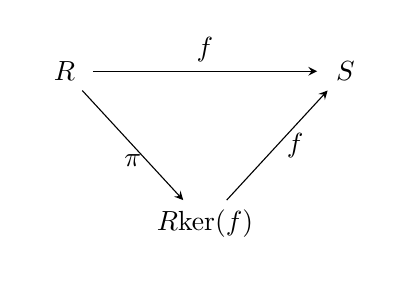
\begin{tikzpicture}
\matrix (m) [matrix of math nodes,row sep=4em,column sep=2em,minimum width=2em]
{
	R &  & S\\
	 & \quot{R}{\ker (f)} &  \\};
\path[-stealth]
(m-1-1) edge node [above] {$f$} (m-1-3)
(m-1-1) edge node [below] {$\pi$} (m-2-2)
(m-2-2) edge node [right] {$\cls{f}$} (m-1-3);
\end{tikzpicture}
\caption{Diagrama que queremos probar como conmutativo.}
\label{fig:Teorema1Isomorfia:Diag1}
\end{wrapfigure}

Queremos probar que el diagrama de la \fref{fig:Teorema1Isomorfia:Diag1} es conmutativo, es decir, que todas las rutas directas en el diagrama con los mismos puntos finales conducen al mismo resultado por composición, o dicho de otra forma, $\forall a \in R$ se cumple que $f(a)=\cls{f}(\pi(a))$

Es decir:
$$ \cls{f}: \quot{R}{\ker (f)} \rightarrow S$$

Es un homomorfismo de anillos.

Definimos $\cls{f}$ de esta manera: $\cls{f}(\pi(a))=f(a)$. vamos a ver que está bien definida, es decir, que sea $a,b \in \quot{R}{\ker (f)}$, entonces $f(a)$ existe y es única (es decir, todos los puntos tienen imágenes y un mismo punto no tiene dos imágenes distintas)

Sabemos que $\pi(a)=\pi(b) \Leftrightarrow a-b \in \ker (f)$ (es decir, $a$ y $b$ pertenecen a la misma clase de equivalencia en $ \quot{R}{\ker (f)}$).

Por tanto, se tiene que $f(a)=f(b)$, $\forall a,b$ con $\pi(a)=\pi(b)$. Ya que si $(a-b) \in \ker (f)$ entonces $f(a-b)=0=f(a)-f(b)$. Esta función no depende del representante de la clase escogido. Con esto garantizamos que está bien definida.

Vamos a ver que $\cls{f}$ es un homomorfismo de anillos:
\begin{enumerate}
	\item $\forall \cls{a},\cls{b} \in \quot{R}{\ker (f)}$, $\cls{f}(\cls{a}+\cls{b})=\cls{f}(\cls{a})+\cls{f}(\cls{b})$.

	Sabemos que $\pi$ es un homomorfismo de anillos por la proposición \ref{prop:pi_homomorfismo}. Por tanto, sea $\pi(a)=\cls{a}$ y $\pi(b)=\cls{b}$, entonces $\cls{a}+\cls{b}=\pi(a)+\pi(b)=\pi(a+b)=\cls{a+b}$.

	Por tanto $\cls{f}(\cls{a}+\cls{b})=\cls{f}(\cls{a+b}) = f(a+b) = f(a)+f(b) = \cls{f}(\cls{a})+\cls{f}(\cls{b})$
	\item $\forall \cls{a},\cls{b} \in \quot{R}{\ker (f)}$, $\cls{f}(\cls{a}\cls{b})=\cls{f}(\cls{a})\cls{f}(\cls{b})$. Se deja como ejercicio para el lector experimentado.
	\item $f\left(1_{\quot{R}{\ker (f)}}\right)=1_{S}$
\end{enumerate}

Para probar que $\quot{R}{\ker (f)} \sim \img (f)$, basta probar que si nos restringimos a las $f \subset S$, entonces $\cls{f}:\quot{R}{\ker (f)} \sim \img (f)$ es biyectiva.

Obviamente es sobreyectiva, ya que nos estamos restringiendo a la imagen. para ver que es inyectiva basta ver que $\ker(\cls{f})=\{0\}$ (Por la proposición \ref{prop:hda_inyectiva}):

$$ \ker(\cls{f})=\set{ \cls{a} \in \quot{R}{\ker (f)}: \cls{f}(\cls{a})=0 } = \set{ \cls{a}\in \quot{R}{\ker (f)}: f(a)=0 } = \{0\} $$
\end{proof}

\begin{prop} \label{prop:FactorizacionHomomorfismo}
Sea $I \subset \ker (f)$. Entonces el siguiente diagrama conmuta:

\begin{center}
\begin{tikzpicture}
\matrix (m) [matrix of math nodes,row sep=4em,column sep=2em,minimum width=2em]
{
	R &  & S\\
	& \quot{R}{I} &  \\};
\path[-stealth]
(m-1-1) edge node [above] {$f$} (m-1-3)
(m-1-1) edge node [below] {$\pi_1$} (m-2-2)
(m-2-2) edge node [right] {$f_1$} (m-1-3);
\end{tikzpicture}
\end{center}

En tal caso, se dice que $f$ factoriza por el homomorfismo $f_1: \quot{R}{I} \rightarrow S$. Esta proposición no es más que una generalización del \nref{thm:IsomorfiaAnillos1}.
\end{prop}

%\begin{proof}
%Entonces $f_1(\pi_1(a))=f(a)$. Cojo $b\in R$ tal que $\pi_1(b)=\pi_1(a) \implies b-a \in I \subset \ker (f) \implies f(b)=f(a)$
%\end{proof}

\begin{prop} \label{prop:FactorizacionHomomorfismo2}
	Sea $f: R \rightarrow S$ un homomorfismo de anillos. Si $f$ factoriza por un homomorfismo $f':\quot{R}{J} \rightarrow S$ entonces $J \subset \ker (f)$
\end{prop}

\begin{proof}
	Lo que estamos haciendo es que sea el siguiente diagrama:

\begin{center}
\begin{tikzpicture}
\matrix (m) [matrix of math nodes,row sep=4em,column sep=2em,minimum width=2em]
{
	R &  & S\\
	& \quot{R}{J} &  \\};
\path[-stealth]
(m-1-1) edge node [above] {$f$} (m-1-3)
(m-1-1) edge node [below] {$\pi_J$} (m-2-2)
(m-2-2) edge node [right] {$g$} (m-1-3);
\end{tikzpicture}
\end{center}

El hecho de que $f$ factorice por el cociente significa que $\exists$ un homomorfismo $g: \quot{R}{J}\rightarrow S$ que hace conmutar el diagrama. Y queremos probar que $J \subset \ker (f)$. Suponemos que no, entonces $\exists b \in J$ tal que $b \notin \ker (f)$.

Como $b \notin \ker (f)$ entonces $f(b) \neq 0$.

Por otro lado, $b \in J$, por tanto, por definición de $\pi_J$, tenemos que $\pi_J(b)=\cls{0}$, y por hipotesis, por ser $g$ un homomorfismo tenemos que $g(\cls{0})=0$.

Por tanto, hemos encontrado un $b \in R$ tal que $f(b)\neq g(\pi_J(b))$. Por tanto el diagrama no conmuta, y llegamos a contradicción, ya que habíamos supuesto que sí conmutaba.
\end{proof}

\begin{defn}[R-álgebra]\label{def:ralgebra}
	Se dice que $B$ es una $R$-álgebra si existe $f:R\longmapsto B$ homomorfismo.
\end{defn}

Ahora vemos algunos ejemplos sobre construir homomorfismos de anillos.
\begin{example}
Quiero construir un homomorfismo de anillos:
$$f: \quot{\rac[x]}{\gen{x^2-2}} \rightarrow \cplex$$

Para ello me basta construir un homomorfismo de anillos de:
$$g: \rac[x] \rightarrow \cplex$$

con $\gen{x^2-2} \subset \ker (g)$, ya que en ese caso, el siguiente diagrama conmutaría, y $g$ sería el homomorfismo de anillos buscado:

\begin{tikzpicture}
\matrix (m) [matrix of math nodes,row sep=4em,column sep=2em,minimum width=2em]
{
	\rac[x] &  & \cplex\\
	& \quot{\rac[x]}{\gen{x^2-2}} &  \\};
\path[-stealth]
(m-1-1) edge node [above] {$g$} (m-1-3)
(m-1-1) edge node [below] {$\pi$} (m-2-2)
(m-2-2) edge node [right] {$f$} (m-1-3);
\end{tikzpicture}

Tenemos que $\gen{x^2-2}=\{ p(x)\cdot(x^2-2):p(x) \in \rac[x] \}$. Por tanto, si $x$ va a $\pm \sqrt{2}$, nos aseguramos que $\forall q(x) \in \gen{x^2-2}$, $g(q(x))=q(\pm \sqrt{2})=0$, y que, entonces $ \gen{x^2-2} \subset \ker (g)$. Con esto, usando el primer teorema de isomorfía, ya tenemos definido el homomorfismo buscado $f: \quot{\rac[x]}{\gen{x^2-2}} \rightarrow \cplex$.
\end{example}

\begin{example}
Quiero construir un homomorfismo de anillos:
$$f: \quot{\rac[x,y]}{\gen{xy-1}} \rightarrow \cplex$$

Para ello me basta construir un homomorfismo de anillos de:
$$g: \rac[x,y] \rightarrow \cplex$$

con $\gen{xy-1} \subset \ker (g)$, ya que en ese caso, el siguiente diagrama conmutaría, y $g$ sería el homomorfismo de anillos buscado:

\begin{tikzpicture}
\matrix (m) [matrix of math nodes,row sep=4em,column sep=2em,minimum width=2em]
{
	\rac[x,y] &  & \cplex\\
	& \quot{\rac[x,y]}{\gen{xy-1}} &  \\};
\path[-stealth]
(m-1-1) edge node [above] {$g$} (m-1-3)
(m-1-1) edge node [below] {$\pi$} (m-2-2)
(m-2-2) edge node [right] {$f$} (m-1-3);
\end{tikzpicture}

Me basta enviar la $x$ a un $a\neq 0$ y la $y$ a $a^{-1}$. Es decir, defino $g$ de modo que $g(x)=a$ y $g(y)=a^{-1}$ para algun $a \in \cplex$. De esa manera, todos los $p(x,y) \in \gen{xy-1}$ cumplen que $g(p(x,y))=(p(a\cdot a^{-1}))=0$. Y entonces $ \gen{xy-1} \subset \ker (g)$. Con esto, usando el primer teorema de isomorfía, ya tenemos definido el homomorfismo buscado $f: \quot{\rac[x,y]}{\gen{xy-1}} \rightarrow \cplex$.
\end{example}



%%% Clase 11/2

\begin{theorem}[Segundo teorema de isomorfía][Teorema\IS 2º de isomorfía] \label{thm:IsomorfiaAnillos2} Sean $I ⊂ J ⊂ R$ ideales de un anillo $R$. Entonces \[ \quot{R}{J} \simeq \frac{\quot{R}{I}}{\quot{J}{I}} \]
\end{theorem}

\begin{proof}

Como $I$ es ideal de $R$, entonces:
\[ \appl{\pi}{R}{\quot{R}{I}} \]
es un homomorfismo de anillos sobreyectivo y $\ker(\pi)=I$. Además, como $J,I$ son ideales y $I\subset J \subset R$, entonces $\quot{J}{I}$ es un ideal de $\quot{R}{I}$, por tanto:
\[
	\pi_1: \quot{R}{I} \rightarrow \quot{\quot{R}{I}}{\quot{J}{I}}=S
\]
es también un homomorfismo de anillos sobreyectivo y $\ker(\pi_1)=\quot{J}{I}$.

Por ser $\pi$ y $\pi_1$ sobreyectivos, entonces $\cls{\pi}=\pi_1\cdot\pi$ también es sobreyectivo, por tanto: $\img(\cls{\pi})=\quot{\quot{R}{I}}{\quot{J}{I}}=S$.

Construimos el siguiente diagrama conmutativo:

\begin{center}
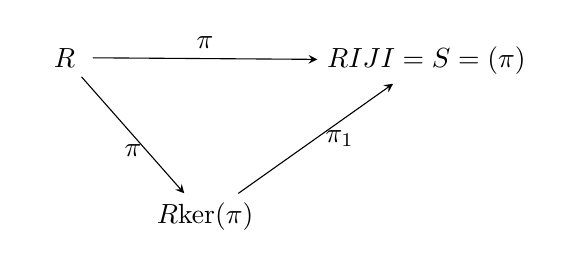
\begin{tikzpicture}
\matrix (m) [matrix of math nodes,row sep=4em,column sep=2em,minimum width=2em]
{
	R &  & \quot{\quot{R}{I}}{\quot{J}{I}} = S = \img(\cls{\pi})\\
	& \quot{R}{\ker(\cls{\pi})} &  \\};
\path[-stealth]
(m-1-1) edge node [above] {$\cls{\pi}$} (m-1-3)
(m-1-1) edge node [below] {$\pi$} (m-2-2)
(m-2-2) edge node [right] {$\pi_1$} (m-1-3);
\end{tikzpicture}
\end{center}

A este diagrama le podemos aplicar el primer teorema de isomorfía y concluir que:

$$ \quot{R}{\ker(\cls{\pi})} \simeq  \quot{\quot{R}{I}}{\quot{J}{I}} $$

Vamos a ver qué es $\ker(\cls{\pi})$:

\begin{itemize}
	\item $\ker(\pi)=\{r \in I\}$. Por tanto, $\forall r \in \ker(\pi)$, $\pi(r)=0$, y por tanto, $\pi_1(0)=0$ y $\pi_1(\pi(r))=\cls{\pi(r)}=0$. Por tanto, $I \subset \ker(\cls{\pi})$.
	\item $\ker(\pi_1)=\{ r \in \quot{J}{I}\}$, que al fin y al cabo son elementos que pertenecen a $J$.
\end{itemize}

Como $I \subset J$, concluimos que $\ker(\cls{\pi}) = J$ y que:

$$ \quot{R}{J} \simeq  \quot{\quot{R}{I}}{\quot{J}{I}} $$

\end{proof}

\begin{corol} Sea $\appl{f}{R}{S}$ un homomorfismo de anillos y sea $\pideal ⊂ S$ un ideal primo. Entonces $\inv{f}(\pideal)$ también es un ideal primo.
\end{corol}

\begin{proof} Vamos a considerar la cadena de homomorfismos:

\begin{tikzpicture}
\matrix (m) [matrix of math nodes,row sep=4em,column sep=2em,minimum width=2em]
{
	R &  &  \quot{S}{\pideal}\\
	& S &  \\};
\path[-stealth]
(m-1-1) edge node [above] {$g$} (m-1-3)
(m-1-1) edge node [below] {$f$} (m-2-2)
(m-2-2) edge node [right] {$\pi$} (m-1-3);
\end{tikzpicture}

$R \xrightarrow{f} S \xrightarrow{π} \quot{S}{\pideal}$, y sea $g = π ○ f$. Por el primer teorema de isomorfía, sabemos que \[ \quot{R}{\ker g} \simeq \img g ⊂ \quot{S}{\pideal} \]

Ahora bien, por ser $\pideal$ primo entonces $\quot{S}{\pideal}$ es un dominio de integridad (proposición \ref{prop:3_propiedades_anillos_cocientes}), y por lo tanto $\quot{R}{\ker g}$ también lo será. Vemos ahora qué es el núcleo de $g$: \[ \ker g = \set{r ∈ R \tq g(r) = π(f(r)) = 0} \]

Dado que $\ker π = \pideal$, para que $r$ esté en el núcleo tenemos que tener que $f(r) ∈ \pideal$, luego $\ker g = \inv{f}(\pideal)$.

Nos falta comprobar que $\inv{f}(\pideal)$ no es el total. Pero si fuese igual, entonces $1_R ∈ \inv{f}(\pideal) \implies f(1) ∈ \pideal$, que no puede ser por ser $\pideal$ primo y $\pideal \subsetneq S$. \textcolor{red}{no tengo muy claro por qué tenemos que comprobar esto, ya que la proposición \ref{prop:3_propiedades_anillos_cocientes} nos lo debería dar directamente}. \noteby{Guille}{Creo que no es lo mismo, aquí estamos con la imagen inversa, lo de la \fref{prop:3_propiedades_anillos_cocientes} lo hemos usado antes para ver que $\quot{S}{\pideal}$ es un dominio de integridad.}
\end{proof}

\begin{example}[Ideales primos y maximales en el cociente]

Antes habíamos visto que cualquier ideal maximal es primo, por lo que la preimagen de un ideal maximal será un ideal primo. Ahora bien, ¿será maximal igualmente? Vamos a comprobarlo.

Consideramos $\appl{f}{R}{S}$ un homomorfismo de anillos y sea $m ⊂ S$ un ideal maximal. Entonces $\inv{f}(m)$ es primo, pero no tiene por qué ser maximal. Por ejemplo, si consideramos $ℤ ⊂ ℚ$, vemos que el único ideal maximal de $ℚ$ es $\zerogen$. La preimagen de este ideal es $\zerogen ⊂ ℤ$, que sigue siendo primo pero no maximal.

Como ejemplo contrapuesto, si consideramos la inclusión $ℤ \hookrightarrow ℤ[x]$ y $p = \gen{2,x} ⊂ ℤ[x]$, vemos que $p$ es primo y maximal, y que además la preimagen de $p$ es $\gen{2} ⊂ ℤ$, que sí es maximal. Pero, como decíamos antes, esto no ocurre siempre y tendremos que comprobarlo.
\end{example}

\begin{example}[La imagen de un ideal primo no tiene por qué ser ideal]

El corolario anterior sólo funciona con preimágenes, no nos vale la imagen directa. Si consideramos por ejemplo la inclusión de $ℤ$ en $ℚ$, el ideal generado por $\gen{2} ⊂ ℤ$ es todo $ℚ$, que no es primo.

Otro ejemplo. Consideramos $ℚ[x] \hookrightarrow \quot{ℚ[x,y]}{\gen{y^2-x}}$. Sabemos que $\gen{x} ⊂ ℚ[x]$ es primo. Ahora bien, pasando al cociente tenemos que \[ \quot{ℚ[x,y]}{\gen{y^2-x, x}} \simeq \quot{ℚ[y]}{\gen{y^2}} \] que obviamente no es un dominio de integridad, por lo que $\cls{\gen{x}}$ no es primo.
\end{example}

Los ejemplos anteriores nos muestran algo que en general no es cierto, aunque sí se va a cumplir si el homomorfismo que consideramos es uno especial: el paso al cociente.

\begin{prop} Sea $I ⊂ R$ un ideal, y consideramos el homomorfismo $\appl{π}{R}{\quot{R}{I}}$. Sea $p ⊂ R$ un ideal primo que contenga a $I$. Entonces $π(p)$ es un ideal primo en $\quot{R}{I}$.
\end{prop}

\begin{proof} Sabemos que, por ser π un paso al cociente y por lo tanto sobreyectiva, $π(p)$ es un ideal, que de hecho es $π(p) = \quot{p}{I}$. Para saber si es primo, tomamos el cociente $\frac{\quot{R}{I}}{\quot{p}{I}}$. Pero por el \nref{thm:IsomorfiaAnillos2}, eso es isomorfo a $\quot{R}{p}$, que es un dominio de integridad, por lo que  $\frac{\quot{R}{I}}{\quot{p}{I}}$ también lo es y entonces $\quot{p}{I}$ es primo.

Por otro lado, si $q ⊂ \quot{R}{I}$ es primo, entonces $\inv{π}(q)$ es un ideal primo en $R$ que además contiene a $I$.
\end{proof}

En el fondo, esta proposición nos dice que la correspondencia biyectiva del paso al cociente va más allá de lo que habíamos comentado antes, ya que también hay una identificación entre los ideales primos de $R$ que contienen a $I$ y los ideales primos de $\quot{R}{I}$. Es decir, que el paso al cociente respeta no sólo inclusiones y maximales, sino también primalidad. De aquí podremos deducir que también hay correspondencia biyectiva entre primos minimales de $R$ que contienen a $I$ y los primos minimales de $\quot{R}{I}$. Por tanto:

\begin{prop}\label{prop:correspondencia_biyectiva}
\textbf{IMPORTANTE:}  Esto viene genial para los ejercicios. Sea $\pi: R \longmapsto \quot{R}{I}$ tenemos que hay una correspondencia biyectiva entre:
\begin{enumerate}
	\item Los ideales \textbf{maximales} en $R$ que contengan a $I$ y los ideales \textbf{maximales} de $\quot{R}{I}$.
	\item Los ideales \textbf{primos} en $R$ que contengan a $I$ y los ideales \textbf{primos} de $\quot{R}{I}$.
	\item Los ideales \textbf{primos minimales} en $R$ que contengan a $I$ y los ideales \textbf{primos minimales} de $\quot{R}{I}$.
\end{enumerate}
\end{prop}

Todo esto que hemos visto nos sirve para demostrar algo que comentamos antes, que es una forma de hallar el radical de un ideal a través de los ideales primos.

\begin{prop} Sea $R$ un anillo. Entonces su radical es \[ \sqrt{I} = \bigcap_{\substack{p ⊂ R\text{ primo} \\ I ⊂ p}} p\]
\end{prop}

\begin{proof} Lo podemos demostrar a través del paso al cociente. Si $f ∈ \sqrt{I}$ entonces $∃n ∈ ℕ$ tal que $f^n ∈ I$. Pasando al cociente por $I$, tenemos que igualmente $\cls{f}^n = \cls{0} ∈ \quot{R}{I}$. Por lo tanto, hay una correspondencia \begin{align*}
R &\longmapsto \quot{R}{I} \\
\sqrt{I} &\longmapsto \nil \quot{R}{I} \\
\bigcap_{\substack{p ⊂ R\text{ primo} \\ I ⊂ p}} &\longleftrightarrow \bigcap_{\substack{p ⊂ {R}/{I} \\ p \text{ primo}}} p
\end{align*}
\end{proof}

\begin{example}[Estudio de ideales a través del paso al cociente]
Vamos a ver todavía más ejemplos de que el paso al cociente es útil. Consideramos $ℚ[x,y]$ y $I = \gen{x^2, xy}$. ¿Cuáles son los ideales primos que  contienen a $I$? Supongamos que $p ⊂ R$ es primo y contiene a $I$.

Como $x^2 ∈ I$, necesariamente $x ∈ p$. Por otro lado, $\gen{x}$ es primo por ser $\quot{ℚ[x,y]}{\gen{x}} \simeq ℚ[y]$ un dominio de integridad. Luego todo primo $p ⊃ I$ contiene necesariamente al ideal primo $\gen{x}$, que de hecho es el mínimo (no hay ningún ideal contenido en él y que sea más pequeño). Por lo tanto $\sqrt{I} = \gen{x}$.

Pero, ¿cómo describimos todos los ideales primos que contienen a $I = \gen{xy, x^2}$? Como hemos visto que todo primo $p ⊃ I$ necesariamente ha de contener a $\gen{x}$, sólo tenemos que buscar los ideales primos en $ℚ[x,y]$ que contengan a $\gen{x}$. Esto es equivalente a buscar los ideales primos en $\quot{ℚ[x,y]}{\gen{x}} \simeq ℚ[y]$, que esto ya sabemos hacerlo: los ideales primos en $ℚ[y]$ son \zerogen y los generados por un polinomio irreducible en $y$. Por lo tanto, los primos que contienen a $I$ serán de la forma $\gen{x, p(y)}$ con $p(y)$ irreducible. De hecho, estos son maximales.

Ahora, la pregunta del millón: ¿por qué estamos haciendo todos estos líos? De nuevo, vayámonos a la geometría. Consideramos en el plano afín los puntos que cumplen que $x^2 = 0$ y que $xy = 0$. Lo que nos sale es el eje $x = 0$ corresponde con el hecho de que $\sqrt{I} = 0$. ¿Y qué tienen que ver los ideales de la forma $\gen{x, p(y)}$? Corresponden a los puntos de la recta $y = 0$ cuando $p$ es de grado $1$. De modo que buscar los maximales y los primos tienen un significado.
\end{example}


% -*- root: ../AlgebraConmutativa.tex -*-
\chapter{Anillos II}

\section{Módulos sobre anillos}
Sea $R$ un anillo, diremos que $M$ es un \concept{{$R$}-módulo} o módulo sobre $R$ si se cumplen las siguientes condiciones:
\begin{enumerate}
	\item $(M,+)$ es un grupo abeliano.
	\item Hay una operación externa sobre $M$.
		\begin{align*}
			R×M & \longmapsto  M \\
			(r,m) & \longmapsto  r\cdot m \\
		\end{align*}

	tal que se cumplen las siguientes propiedades, a las que llamaremos \textbf{propiedades romanas} o \textbf{propiedades sensatas}:
	\begin{itemize}
		\item $\forall r \in R, \forall m,m' \in M$: $r(m+m')=rm+rm'$.
		\item $\forall r,r' \in R, \forall m \in M$: $(r+r')m=rm+r'm$.
		\item $\forall r,r' \in R, \forall m \in M$: $r(r'm)=(rr')m$.
		\item $\forall m \in M$, $\one_R\cdot m = m$.
	\end{itemize}
\end{enumerate}

\begin{example}
	\begin{itemize}
		\item Si $R$ es un cuerpo $\implies$ cualquier espacio vectorial sobre $R$ es un módulo sobre $R$.
		\item Si $I \subset R$ es un ideal $\implies$ $I$ es un $R$-módulo. Por tanto, en particular $R$ es un $R$-módulo.
		\item Sea $f: R \longmapsto S$ un homomorfismo de anillos, sea $J \subset S$ un ideal $\implies$ $J$ es un $R$-módulo.
		\begin{proof}
			De esté último ejemplo, tenemos que ver que se cumplen las propiedades de los $R$-módulos:
			\begin{enumerate}
				\item $(J,+)$ es un subgrupo por ser ideal.
				\item Definimos la operación externa:
				\begin{align*}
					R×J & \longmapsto  J \\
					(r,a) & \longmapsto  f(r)\cdot a \\
				\end{align*}

				Defino $r\cdot a=f(r)\cdot a$. Ahora tenemos que ver que se cumplen las propiedades sensatas, demostramos la primera y las demás las dejamos como ejercicio para el lector con mucho tiempo libre:
				\begin{itemize}
					\item $\forall r \in R, \forall a,a' \in J$, $r(a+a')=ra+ra'$:

					Por definición de la operación externa tenemos que: $r(a+a')=f(r)(a+a')$. Por la propiedad distributiva de $S$ tenemos que $f(r)(a+a')=f(r)a+f(r)a'$. Aplicando de nuevo la definición de producto externo $f(r)a+f(r)a'=ra+ra'$.
				\end{itemize}
			\end{enumerate}
		\end{proof}
	\end{itemize}
\end{example}

Más ejemplos:
\begin{example}
	\begin{itemize}
		\item El ideal $\gen{x}$ en $\ent[x]$ es un $\ent$-módulo.
		\item Sea $I \subset R$ un ideal, sea $\pi:R\longmapsto \quot{R}{I}$ un homomorfismo de anillos, todo ideal de $\quot{R}{I}$ es un $R$-módulo.
		\item Sea $f:R \longmapsto S$ un homomorfismo de anillos. Entonces S es también un $R$-módulo.
		\item Todo anillo $R$ es un $\ent$-módulo. Para ello basta comprobar que siempre hay un homomorfismo de anillos de $\ent$ en R.
		\begin{align*}
			g:\ent &\longmapsto  R\\
			1 & \longmapsto \one_R \\
			m & \longmapsto  m\cdot \one_R \\
		\end{align*}

		Con esto defino el homomorfismo porque 1 genera $\ent$ como grupo.

		Es más, todo anillo $R$ contiene una copia de $\ent$ o una copia de algún $\ent_n$. Basta observar que $\ent/\ker(g) \simeq \img(g) \subset R$. Por tanto hay dos casos:
		\begin{enumerate}
			\item Si $\ker(g)=(0) \implies \ent \simeq \img(g) \subset R$
			\item Si $\ker(g)=\gen{n}\implies \ent_n \simeq \img(g) \subset R$ para $n\in \ent$ con $n\neq0$ y $n\neq 1,-1$ (porque $1\notin \ker(g)$).
		\end{enumerate}
	\item En $\ent_{10}$ cogemos $M=\gen{2}=\{\cls{0},\cls{2},\cls{4},\cls{6},\cls{8} \}$

	M es también un $\ent_5$-módulo (aparte de un $\ent_{10}$-módulo y un $\ent$-módulo), ya que:
	\begin{enumerate}
		\item $(M,+)$ es un grupo abeliano, al ser ideal.
		\item Definimos la operación externa:
		\begin{align*}
			\ent_5 × M & \longmapsto  M \\
			(\cls{a},\cls{m}) & \longmapsto  \cls{a}\cdot \cls{m} =\cls{a\cdot m} \\
		\end{align*}

		Vamos a ver que este producto está bien definido, es decir, que no depende de los representantes escogidos: $\cls{a}=a+5l$, y $\cls{m}=2n+10k$. Operamos:
		$$\cls{a}\cdot \cls{m}=a2n+10ak+10lm+50lk \underbrace{\equiv}_{mod 10} a2n=\cls{a2n}=\cls{a}\cls{2n}$$

		Vemos que efectivamente esta operación no depende de los representantes obtenidos y por tanto está bien definida. faltaría comprobar las propiedades romanas (o sensatas) y ya está (pero not today).
		\item Sin embargo en el ejemplo anterior $M$ no es un $\ent_3$-módulo. Por ejemplo, en $\ent_3$ es lo mismo 1 que 4. Sin embargo, cogiendo $\cls{2}\in M$, no es lo mismo $4\cdot\cls{2}=8=\cls{8}$ que $1\cdot\cls{2}=2=\cls{2}$.
	\end{enumerate}
	\end{itemize}
\end{example}

\begin{defn}[R-módulo\IS finitamente generado]\label{def:rmodulo_fg}
	Sea $M$ un $R$-módulo, diremos que $M$ es un $R$-módulo finitamente generado si $\exists m_1,\dots,m_s \in M$ tal que $M=\{r_1m_1+\dots+r_sm_s: r_i \in R \}$.

	Es decir $\exists m_1..., m_n \in M$ tales que cada elemento de M es una combinación lineal de esos elementos con coeficientes del anillo escalar R.
\end{defn}

\begin{example}
	\begin{itemize}
	\item Sea $\ent$, cogemos $I=\gen{a}$ con $a\in \ent$. I es un $\ent$-módulo finitamente generado ya que $I=\{na:n \in \ent \}$. Cada elemento de $M$ se puede escribir como $a$ multiplicado por algún elemento de $\ent$.
	\item Sea $K[x]$, cogemos $I \subset K[x]$ con $I=\gen{p(x)}=\{ q(x)p(x): q(x) \in K[x] \}$. $I$ es un $K[x]$-módulo finitamente generado.
	\item Sea $\rac[x,y]$ cogemos $I=\{ p(x,y):p(0,0)=0 \}=\gen{x,y}=\{ xp(x,y)+yr(x,y): p,q \in \rac[x,y] \}$. $I$ es un $\rac[x,y]$-módulo finitamente generado.
	\item $\ent[x]$ no es un $\ent$-módulo finitamente generado.

	\begin{proof}
		Supongamos que $\ent[x]$ fuera finitamente generado como $\ent$-módulo. Entonces $\exists p_1(x),\dots,p_r(x) \in \ent[x]$ tales que $\ent[x]\{ n_1p_1(x)+\dots+n_rp_r(x): n_i \in \ent \}$. Sea $m=\max\{grado(p_i(x)) \} \implies grado(n_1p_1(x)+\dots+n_rp_r(x)) \leq m$. Pero en $\ent[x]$ no hay grado máximo.

		Sin embargo $\ent[x]$ si es una $\ent$-álgebra finitamente generada, o una $\ent$-algebra de tipo finito ya que:
		$$ \ent[x]=\set{ \sum_{i=0}^n a_i x^i: a_i \in \ent, n \in \nat }$$
	\end{proof}
	\item Sea $\rac \subset \rac[\sqrt{2}]$.

	Es un $\rac$-módulo finitamente generado ya que $\rac[\sqrt{2}]=\{ a+b\sqrt{2}:a,b \in \rac \}$.

	Es también una $\rac$-algebra ya que $\rac[\sqrt{2}]=\{ \sum_{i=0}^n a_i(\sqrt{2})^i :a_i \in \rac, n \in \nat \}$
\end{itemize}
\end{example}

\begin{defn}[R-álgebra\IS finitamente generada]\label{def:ralgebra_fg}
	Sea $f: R \longmapsto S$ un homomorfismo de anillos. Entonces $S$ es una $R$-álgebra vía f (ver \ref{def:ralgebra}). Diremos que S es una $R$-álgebra finitamente generada (o de tipo finito) si $\exists \alpha_1,\dots, \alpha_s \in S$ tal que:
	$$ S=\left\{ \sum_{finito} f(a_{i1}\dots a_{ir})\alpha_1^{i1}\dots\alpha_r^{ir}: a_{i1},\dots, a_{ir} \in R \right\} $$
\end{defn}

\begin{example}
	\begin{itemize}
		\item Sea $\real \longmapsto \real[x]$. Tomamos $\alpha_1=x$, y entonces $\real[x]=\left\{ \sum_{i=1}^n a_ix^i: a_i \in \real, n\in \nat  \right\}$
		\item Sea $R \longmapsto R[x_1,\dots,x_n]$ no es un $R$-módulo finitamente generado pero si es una $R$-álgebra de tipo finito, porque podemos coger $\alpha_1=x_1,\dots,\alpha_n=x_n$.
		\item Sea $R \longmapsto R[x_1,...,x_n,...]$ (número infinito de variables) entonces no es ni $R$-módulo ni $R$-álgebra.
		\item Sea $\rac \longmapsto \rac[\sqrt{2}]$ es una $\rac$-álgebra finitamente generada (la genera $\sqrt{2}$) y un $\rac$-módulo finitamente generado (lo genera $\{ 1, \sqrt{2} \}$).
		\item Sea $\real$, es una $\rac$-álgebra pero no es de tipo finito (si lo fuera $\real$ sería numerable). Es un $\rac$-módulo.
	\end{itemize}
\end{example}

\begin{defn}[R-submódulo]
	Sea $M$ un $R$-módulo. Diremos que $N \subset M$ es un $R$-submódulo de $M$ si $N$ es un $R$-módulo.
\end{defn}
\begin{prop}
	Sea $M$ un $R$-módulo y sea $N \subset M$. Entonces $N$ es un $R$-submódulo $\Leftrightarrow$:
	\begin{enumerate}
		\item $N \neq \emptyset$.
		\item Si $n,m \in \nat$, $n-m \in \nat$ (lo que es equivalente a que Si $n,m \in \nat$, $n+m \in \nat$).
		\item $\forall r \in R, \forall n \in N$, $rn \in N$.
	\end{enumerate}
\end{prop}

\begin{defn}[Homomorfismo\IS de R-módulos]
	Sean $M,L$ dos $R$-módulos y sea $f:M\longmapsto L$. Diremos que f es un homomorfismo de $R$-módulos si:
	\begin{enumerate}
		\item $\forall n,m \in M$ se tiene que $f(n+m)=f(n)+f(m)$.
		\item $\forall r \in R,\forall m \in M$, se tiene que $f(rm)=rf(m)$.
	\end{enumerate}
\end{defn}

\begin{defn}[Homomorfismo\IS de R-álgebras]
	Sea $R\subset A,B$ tenemos un homomorfismo $f: A \rightarrow B$, $f$ es homomorfismo de $R$-álgebras si todos los elementos de $R$ van a parar a sí mismos.
\end{defn}

\begin{example}
	Cogemos $R= \ent$, $M=\gen{2}$ y $N=\gen{3}$. El homomorfismo sería:
	\begin{align*}
		f: \gen{2} & \longmapsto  \gen{3}\\
		x & \longmapsto 3x \\
	\end{align*}


	\obs De $\ent \longmapsto \ent$ no se puede hacer ya que $x \longmapsto 3x$ mandaría el \one al 3 y el \one tiene que ir al \one.
\end{example}

\begin{defn}[Núcleo\IS de homomorfismo de R-módulos]
	Sea $f:M \longmapsto N$ un homomorfismo de $R$-módulos. Definimos $\ker(f)=\{ m\in M:f(m)=0 \}$.
\end{defn}

\obs $\ker(f)$ es un submódulo de M. (Si no te lo crees, lo demuestras).

\begin{defn}[Cociente\IS de módulos]
Si $N \subset M$ es un submódulo de M, se define de manera natural el cociente $\quot{N}{M}$, $m,m' \in M$, $m~m'$ si $m-m' \in N$. Y $\quot{M}{N}$ es un $R$-modulo.
\end{defn}

Se deja como ejercicio escribir las versiones del primer y segundo teoremas de isomorfía para módulos.

\section{Tercer Teorema de isomorfía}
\begin{theorem}[Tercer teorema de isomorfía][Teorema\IS 3º de isomorfía] \label{thm:IsomorfiaAnillos3}
	Sean $I$, $J$ ideales en $R$:
	$$ \quot{I+J}{I} \simeq \quot{J}{I \cap J} $$
\end{theorem}
\begin{proof}
	Recordemos que $I+J$ es el ideal más pequeño que contiene a $I$ y a $J$.


	Sea $\pi: R \longmapsto \quot{R}{I}$, sabemos que $\pi$ es sobreyectiva y que $\ker(\pi)=I$. Por tanto, $\pi(I)=0$, y $\pi(I+J)=\pi(J)$ es un ideal.

	Además, pues que $\pi$ no es más que una aplicación de paso al cociente, tenemos que $\pi(J)=\pi(J+I)=\quot{J+I}{I}$. Definimos la siguiente función sobreyectiva:

	$$ \cls{\pi}=\pi|_J: J \longmapsto \quot{J+I}{I}  $$

	Por el primer teorema de isomorfía, se tiene que:
	$$ \quot{J}{\ker(\cls{\pi})} \simeq \quot{J+I}{I} $$

	Entonces vamos a calcular $\ker(\cls{\pi})$. Que serán los elementos de $I$. Pero como no necesariamente esta $I\subset J$, entonces cogemos los elementos de $I$ que también pertenecen a $J$. Es decir $\ker(\cls{\pi})=I \cap J$, por tanto:

	$$ \quot{J}{I \cap J} \simeq \quot{J+I}{I} $$

\end{proof}


\begin{example}
	Cogemos $\gen{4}$ y $\gen{6}$ contenidos en $\ent$. Por el tercer teorema de isomorfía tenemos:
	$$ \quot{\gen{4}+\gen{6}}{\gen{4}}\simeq \quot{\gen{6}}{\gen{6} \cap \gen{4}} $$

	Lo comprobamos:
	$$\quot{\gen{4}+\gen{6}}{\gen{4}} = \quot{\gen{2}}{\gen{4}}=\{ \cls{0} \cls{2} \}$$

	$$ \quot{\gen{6}}{\gen{6} \cap \gen{4}} = \quot{\gen{6}}{\gen{12}} = \{ \cls{0}, \cls{6} \}$$

	El isomorfismo sería:
	\begin{align*}
		\cls{0}  & \longmapsto  \cls{0}\\
		\cls{6} & \longmapsto \cls{2} \\
	\end{align*}
\end{example}

\section{Localización en una parte multiplicativa}
\begin{defn}[Parte\IS multiplicativa]
	Sea $R$ un anillo y sea $S\subset R$ un subconjunto. Diremos que $S$ es una parte multiplicativa en $R$ o un conjunto multiplicativamente cerrado en $R$ si se cumplen las siguientes condiciones:
	\begin{enumerate}
		\item $\one \in S$
		\item $s,s' \in S \implies s\cdot s' \in S$.
	\end{enumerate}
\end{defn}

Por tanto, intuitivamente vemos que

\begin{example}
	\begin{itemize}
		\item Sea $R$, cogemos $S=\{\one \}$
		\item Sea $R$, cogemos $S=U(R)$ (Unidades de R).
		\item Sea $a \in R$, cogemos $S=\{ a^n: n \in \nat \}$.
		\item Sea $p \subset R$ un ideal primo. Cogemos $S=R \setminus p$. Este ejemplo vamos a probarlo, S es una parte multiplicativa porque:
		\begin{enumerate}
			\item $\one \in S$, ya que $\one \notin p$.
			\item $s,s' \in S \implies s\cdot s' \in S$. Si ya que: $s,s' \in S \implies s,s' \notin p \implies s\cdot s' \notin p \implies s\cdot s' \in S$.
		\end{enumerate}
		\item Sea R, cogemos $S= R \setminus \{\{ \text{divisores de 0}\}\cup \{ \zero \} \}$ también es parte multiplicativa.
		\item Sea $R$, y sea $\{p_i\}_{i\in I}$ colección de ideales primos en $R$. Entonces $S=R\setminus \bigcup_{i\in I}p_i$ es una parte multiplicativa.
	\end{itemize}
\end{example}

\subsection{Construcción del localizado de R en una parte multiplicativa S}

Sea $S \subset R$. Construimos $R×S=\{ (r,s): r \in R, s\in S \}$. Podemos pensar en lugar del par $(r,s)$ en la fracción $\frac{r}{s}=s^{-1}r$, de ahí viene la expresión $S^{-1}R$. Necesitaremos además una forma de identificar elementos igual que identificamos fracciones, así que una primera relación de equivalencia en $R×S$ podría ser la siguiente: \( (r,s)\sim(r',s') \iff rs'-r's =0 \label{eq:RelEquivLocalizado_Mala} \)

Podemos definir la operación suma como, dados $(r,s), (r',s')\in R×S$, entonces $(r,s)+(r',s')=(rs',ss')+(r's,s's)=(rs'+r's,ss')$. La operación producto sería la obvia: $(r,s)+(r',s')=(rr',ss')$.

Ahora bien, lo malo de la relación de equivalencia que hemos dado en \eqref{eq:RelEquivLocalizado_Mala} es que nos puede dar problemas. Vamos a tomar $\ent_6$ y $S=\set{ \cls{1},\cls{2},\cls{4}}$ una parte multiplicativa, para construir el localizado $\inv{S}ℤ_6$.

En ese localizado podemos coger $(\cls{3},\cls{1})$ y $(\cls{0},\cls{1})$. Obviamente no están relacionados, ya que $\cls{3}\cdot\cls{1}\neq \cls{1}\cdot\cls{0}$. Podemos hacer una manipulación extra, que es multiplicar por $\cls{2}$ el primer elemento, $(\cls{3}, \cls{1})$. Esto no debería cambiar la relación de equivalencia (sólo hay que mirar la definición de \eqref{eq:RelEquivLocalizado_Mala} para verlo), pero si calculamos, tenemos que $\cls{2} · (\cls{3}, \cls{1}) = (\cls{0}, \cls{2})$ y ahora ambos elementos sí están relacionados: $\cls{0} · \cls{1} = \cls{0} · \cls{2}$. En otras palabras, algo ha fallado en la definición de relación de equivalencia y tenemos que mejorarla.

Esa mejora será definirla de la siguiente forma: \( (r,s) \sim (r', s') \iff ∃s'' ∈ S \tq s''(rs'-r's) = 0 \label{eq:RelEquivLocalizado} \)

Ahora sí podremos probar que es una relación de equivalencia:

\begin{itemize}
\item \textbf{Reflexión}: Es claro que $(r,s) \sim (r,s)$, tomando $s'' = \one ∈ S$.
\item \textbf{Simetría}: Si $(r,s) \sim (r',s')$, entonces $∃s'' ∈ S$ tal que $s'' (rs' - r's) = 0$. Declaramos que $s''$ nos vale para decir que $(r',s') \sim (r,s)$. Sea $a = s''(r's-rs')$. Podemos sumar entonces a esta ecuación la que ya sabemos que se cumple: $s''(rs'-r's) = 0$ y entonces
\begin{align*}
s''(rs'-r's) + s''(r's-rs') &= 0 + a \\
s''(rs'-r's + r's-rs') &= a \\
0 &= a
\end{align*}, por lo que efectivamente $(r',s') \sim (r,s)$.
\item \textbf{Transitividad}: No se me ocurre como probarla ahora mismo.
\end{itemize}

Así, Definimos el siguiente anillo:
 $$S^{-1}R = \left( \quot{R×S}{\sim},+,\cdot \right)$$

En el que encontramos:
\begin{itemize}
	\item Elemento neutro para $+$, que es el $(0,s)$, $\forall s \in S$ (todos ellos conforman la misma clase de equivalencia, así que no se viola la unicidad).
	\item Identidad para $\cdot$, que es $(1,1)$.
	\item Sea $(s,1) \in S^{-1}R$, su inverso es $(1,s) \in S^{-1}R$.
\end{itemize}

Vamos a ver $R$ en $S^{-1}R$. Para ello construimos una función de $R$ en $S^{-1}R$ de la siguiente manera:
\begin{align*}
	R & \longmapsto  S^{-1}R\\
	r & \longmapsto (r,1) \\
\end{align*}

Esta aplicación es un homomorfismo de anillos, y podremos estudiar propiedades de los elementos de $\inv{S}R$ a través de él.

Por ejemplo, podemos estudiar su núcleo, que serán los elementos cuya imagen sea la clase de $0_{\inv{S} R}$, que es de la forma $(0,s)$. Simplemente aplicando $f$, tenemos que tener $(r, 1) \sim (0,s)$, lo que nos lleva a la definición verdaderamente útil del núcleo: \[ \ker f = \set{r ∈ R \tq ∃s ∈ S,\, s'r = 0_R} \]

Este homomorfismo no siempre es inyectivo.

\begin{prop}
	$S^{-1}R=\{ 0 \} \Leftrightarrow 0 \in S \Leftrightarrow S$ contiene nilpotentes.
\end{prop}

\begin{prop}
	Si $S^{-1}R \neq \{ 0 \} \implies f(s)$ es invertible en $S^{-1}R\; \forall s \in S$
\end{prop}

\begin{example} \textbf{Importante para practicar con parte multiplicativa y repasar lo anterior}
	Sea $R = \ent_6$ y $S=\{ \cls{1}, \cls{2}, \cls{4} \}$

	Vamos a estudiar $S^{-1}\ent_6$, para ello seguimos los siguientes pasos:

	Definimos el homomorfismo tal y como hemos dicho:
	\begin{align*}
		f: \ent_6 & \longmapsto  S^{-1}\ent_6\\
		\cls{0} & \longmapsto (\cls{0},\cls{1}) \\
		\cls{n} & \longmapsto (\cls{n},\cls{1}) \\
	\end{align*}

Calculamos el núcleo: $\ker(f)=\{ r \in R: \exists s' \in S: s'r=0 \}$. Es decir
$$\ker(f) = \{ r \in \ent_6: \exists s' \in \{ \cls{1}, \cls{2}, \cls{4} \}: s'r=0_{\ent_6} \} = \{ \cls{0}, \cls{3}\}$$

\textcolor{blue}{Demostracion a saco (cuentas tontas):
	\begin{itemize}
		\item $\cls{0} \in \ker(f)$ ya que $s'\cls{0}=\cls{0}$, $\forall s' \in S$
		\item $\cls{1} \notin \ker(f)$ ya que $s'\cls{1}\neq\cls{0}$, $\forall s' \in S$: $\cls{1}\cdot\cls{1}=\cls{1}$, $\cls{2}\cdot\cls{1}=\cls{2}$ y $\cls{4}\cdot\cls{1}=\cls{4}$
		\item $\cls{2} \notin \ker(f)$ ya que $s'\cls{2}\neq\cls{0}$, $\forall s' \in S$: $\cls{1}\cdot\cls{2}=\cls{2}$, $\cls{2}\cdot\cls{2}=\cls{4}$ y $\cls{4}\cdot\cls{2}=\cls{2}$
		\item $\cls{3} \in \ker(f)$ ya que $s'\cls{3}=\cls{0}$ cogiendo $s'=\cls{2}$ o $s'=\cls{4}$
		\item $\cls{4} \notin \ker(f)$ ya que $s'\cls{4}\neq\cls{0}$, $\forall s' \in S$: $\cls{1}\cdot\cls{4}=\cls{4}$, $\cls{2}\cdot\cls{4}=\cls{2}$ y $\cls{4}\cdot\cls{4}=\cls{4}$
		\item $\cls{5} \notin \ker(f)$ ya que $s'\cls{5}\neq\cls{0}$, $\forall s' \in S$: $\cls{1}\cdot\cls{5}=\cls{5}$, $\cls{2}\cdot\cls{5}=\cls{4}$ y $\cls{4}\cdot\cls{5}=\cls{2}$
	\end{itemize}}

	Ahora vamos a usar el primer teorema de isomorfía. Por el cual sabemos que existe un homomorfismo de anillos:
	$$\cls{f}: \quot{\ent_6}{\gen{\cls{3}}} \longmapsto S^{-1}\ent_6$$

	\textbf{Notacion:}
	\begin{itemize}
		\item $\ent_6 = \quot{\ent}{\gen{6}}= \quot{\ent}{6 \ent}$.
		\item En este caso $\gen{\cls{3}}$ es el ideal generado por $\cls{3}$ dentro del ideal $6\ent=\gen{6}$ en $\ent$. Es decir, que en este caso se cumple: $\gen{\cls{3}}=\quot{3\ent}{6\ent} = \{ \cls{0}, \cls{3}\}$ como hemos visto.
	\end{itemize}

	Ahora aplicamos el segundo teorema de isomorfía. Para ello necesitamos $I \subset J \subset R_1$. Cogemos $R_1 = \ent$, $J=\gen{3}$ e $I=\gen{6}$. Por el segundo teorema de isomorfía:

	$$ \quot{\ent_6}{\gen{\cls{3}}} \simeq \quot{\quot{\ent}{\gen{6}}}{\quot{\gen{3}}{\gen{6}}} \underbrace{\simeq}_{2º \text{tma isomorfía} } \quot{\ent_6}{\gen{3}} \simeq \ent_3$$

	Ahora volvemos a aplicar el primer teorema de isomorfía, pero la segunda parte, la que nos dice que: $\quot{R}{\ker(f)} \simeq \img(f)$. En nuestro caso tenemos $R=\ent_6$, y $\ker(f)=\gen{\cls{3}}$, y como acabamos de ver  $\quot{\ent_6}{\gen{\cls{3}}}$ es isomorfo $\ent_3$. Por tanto no queda otra que:

	$$\img(f) \simeq \ent_3$$

	Sabiendo podemos definir $f$ de forma mucho más precisa:
	\begin{align*}
		f: \ent_6 & \longmapsto  S^{-1}\ent_6 \simeq \ent_3\\
		\cls{0} & \longmapsto (\cls{0},\cls{1}) \\
		\cls{1} & \longmapsto (\cls{1},\cls{1}) \\
		\cls{2} & \longmapsto (\cls{2},\cls{1}) \\
		\cls{3} & \longmapsto (\cls{0},\cls{1}) \\
		\cls{4} & \longmapsto (\cls{1},\cls{1}) \\
		\cls{5} & \longmapsto (\cls{2},\cls{1}) \\
	\end{align*}

	Ahora podemos ver las equivalencias entre los elementos de $S^{-1}\ent_6$, algunos ejemplos son:
	\begin{itemize}
		\item $(\cls{1},\cls{4})\equiv (\cls{1},\cls{1})$ porque $\cls{1}\cdot \cls{4} = \cls{4} = \cls{1} =\cls{1}\cdot \cls{1}$.
		\item $(\cls{2},\cls{1}) \equiv (\cls{1},\cls{2})$ ya que $\cls{2}\cdot \cls{2} = \cls{4} = \cls{1} =\cls{1}\cdot \cls{1}$.
		\item $(\cls{4},\cls{1}) \equiv (\cls{2},\cls{2})$ ya que $\cls{4}\cdot \cls{2} = \cls{8} = \cls{2} =\cls{1}\cdot \cls{2}$.
		\item $(\cls{2}, \cls{2}) = (\cls{2},\cls{1}) \cdot (\cls{1},\cls{2}) \equiv (\cls{4},\cls{1}) $.
		\item $(\cls{2},\cls{1}) \cdot (\cls{2},\cls{1}) = (\cls{4},\cls{1}) = (\cls{1},\cls{1})$. Por tanto $(\cls{2},\cls{1})^{-1}=(\cls{2},\cls{1}) = (\cls{1},\cls{2})$. Ya que $(\cls{2},\cls{1}) \equiv (\cls{1},\cls{2})$.
	\end{itemize}
	\end{example}

	\begin{theorem}[Propiedad universal de la localización] \label{thm:PropUniversalLoc}
		Sea $S\subset R$ una parte multiplicativa. Suponemos $S^{-1}R \neq \{0\}$. Sea $f:R \longmapsto B$ un homomorfismo de anillos tal que $\forall s \in S$, $f(s)$ es invertible. Entonces existe un único homomorfismo de anillos $g: S^{-1}R \longmapsto B$ tal que el siguiente diagrama conmuta:

		\begin{center}
		\begin{tikzpicture}
\matrix (m) [matrix of math nodes,row sep=4em,column sep=2em,minimum width=2em]
{
	R &  &  B\\
	& S^{-1}R &  \\};
\path[-stealth]
(m-1-1) edge node [above] {$f$} (m-1-3)
(m-1-1) edge node [below] {$\psi$} (m-2-2)
(m-2-2) edge node [right] {$g$} (m-1-3);
\end{tikzpicture}

		\end{center}
	\end{theorem}

	\begin{proof}
		Hay que demostrar que $g$ existe y es único. Tenemos lo siguiente:

		\begin{tikzpicture}
		\matrix (m) [matrix of math nodes,row sep=4em,column sep=2em,minimum width=2em]
		{
			R &  &  B\\
			& S^{-1}R &  \\};
		\path[-stealth]
		(m-1-1) edge node [above] {$f$} (m-1-3)
		(m-1-1) edge node [below] {$\psi$} (m-2-2);
		\end{tikzpicture}

		\proofpart{Unicidad}

		Primero probamos que si existe $g$ que hace conmutar el diagrama, debe ser único. Tomamos entonces una aplicación de la siguiente forma:
		\begin{align*}
			g: S^{-1}R & \longmapsto  B\\
			\frac{r}{s} & \longmapsto g\left( \frac{r}{s} \right)=g(r)\cdot g(s)^{-1} \\
		\end{align*}

		Fijamos entonces un $a ∈ R$ y hacemos los dos caminos, por $f$ y por $g○ψ$:

		\begin{center}
			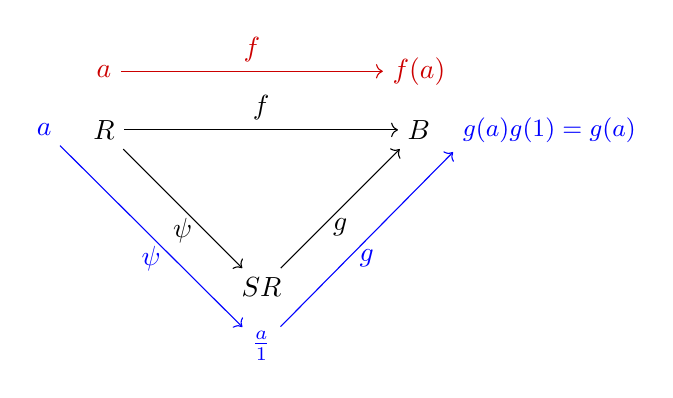
\begin{tikzpicture}
			\node (R) at (0,0) {$R$};
			\node (SR) at (2,-2) {$\inv{S}R$};
			\node (B) at (4, 0) {$B$};

			\draw[->] (R) -- node[midway, below] {$\psi$} (SR);
			\draw[->] (SR) -- node[midway, below] {$g$} (B);
			\draw[->] (R) -- node[midway, above] {$f$} (B);

			\node[blue, xshift = -0.5cm] (A) at (R.west) {$a$};
			\node[blue, xshift = 0.7cm, anchor = west] (AB) at (B.west) {\small $g(a)·\inv{g(1)} = g(a)$};
			\node[blue, yshift=-0.5cm] (A1) at (SR.south) {$\frac{a}{1}$};

			\draw[->, blue] (A) -- node[midway, below] {$\psi$} (A1);
			\draw[->, blue] (A1) -- node[midway, below] {$g$} (AB.south west);

			\node[red!80!black, yshift = 0.5cm] (FA) at (R.north) {$a$};
			\node[red!80!black, yshift = 0.5cm] (FB) at (B.north) {$f(a)$};

			\draw[->, red!80!black] (FA) -- node[midway, above] {$f$} (FB);
			\end{tikzpicture}
		\end{center}

		Por tanto, como el diagrama conmuta $g(a)=f(a)$, lo que nos deja fijo el comportamiento de $g$ en los elementos de la forma $\frac{a}{1}$ con $a ∈ R$. Nos falta saber qué ocurre con los que no son de esa forma, y saber si ahí también tenemos una única posibilidad de tomar $g$.

		Para eso, sólo tenemos que ver qué ocurre a los elementos de la forma $\frac{1}{s}$. Operando: \[ g(\frac{1}{s})=g(1)g(s^{-1})=g(s^{-1})=g(s)^{-1}=f(s)^{-1} \], ya que por hipótesis $f(s)$ con $s ∈ S$ son elementos invertibles. Por lo tanto, $g$ es única y depende solamente de la elección de la $f$ de partida.

		\proofpart{Existencia}

		Ahora vamos a probar que existe esa $g$. Si $g$ existiese tendríamos $g\left( \frac{r}{s}\right)=f(r)f(s)^{-1}$. Tenemos que ver que $g$ está bien definida (que dos elementos iguales no tengan imágenes distintas), es decir, que la expresión anterior no dependa del representante escogido.

		Supongamos que $\frac{r}{s} \equiv \frac{r'}{s'}$, hay que ver que $g\left(\frac{r}{s}\right)=g\left(\frac{r'}{s'}\right)$. Es decir, que $f(r)f(s)^{-1}=f(r')f(s')^{-1}$.

		Como  $\frac{r}{s} \equiv \frac{r'}{s'}$, entonces existe $s'' \in S$ tal que $s''(rs'-sr')=0$ en $R$. Aplicando f nos queda:
		$$f(s''(rs'-sr'))=f(s'')\left( f(r)f(s')-f(s)f(r') \right)=0$$

		Por hipótesis $f(s'')$ es invertible, por tanto, es una unidad en $B$, entonces no es un divisor de 0 y por tanto:
		$$f(r)f(s')-f(s)f(r')=0 \implies f(r)f(s')=f(s)f(r')$$

		Y multiplicando por la inversa de $f(s')$ y de $f(s)$, nos queda $f(r)f(s)^{-1}=f(r')f(s')^{-1}$.
	\end{proof}

	\begin{example}
		Sea $\rac[x]$, cogemos como parte multiplicativa $S=\{x^n\}$.

		Los elementos de $S^{-1}\rac[x]$ serán de la forma $\frac{p(x)}{x^m}$.

		\notacion $S^{-1}\rac[x]=\rac[x]_{\{x\}}$

		Defino el siguiente diagrama:

		\begin{center}
		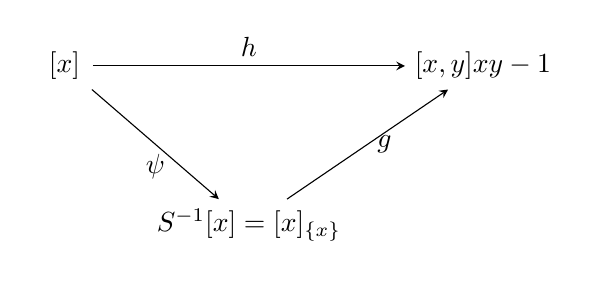
\begin{tikzpicture}
		\matrix (m) [matrix of math nodes,row sep=4em,column sep=2em,minimum width=2em]
		{
			\rac[x] &  & \quot{\rac[x,y]}{\gen{xy-1}} \\
			& S^{-1}\rac[x]=\rac[x]_{\{x\}}  &  \\};
		\path[-stealth]
		(m-1-1) edge node [above] {$h$} (m-1-3)
		(m-1-1) edge node [below] {$\psi$} (m-2-2)
		(m-2-2) edge node [right] {$g$} (m-1-3);
		\end{tikzpicture}
		\end{center}

		Vemos que $\cls{x}\cls{y}=\cls{1} \implies x^{-1}=y \implies (x^m)^{-1}=y^m$. Con esto hemos visto que $h(s)$ es invertible $\forall s \in S$.

		La propiedad universal me dice que tengo un único homomorfismo $g: \rac[x]_{\{x\}}\longmapsto \quot{\rac[x,y]}{\gen{xy-1}}$

	\end{example}

	\begin{theorem} \label{thm:PropsLocalizacion}
		Sea $S \subset R$ una parte multiplicativa. El homomorfismo de paso al localizado $\psi:R \longmapsto S^{-1}R$ tiene las siguientes propiedades:
		\begin{enumerate}
			\item Si $s\in S$, $\psi(s)$ es invertible en $S^{-1}R$.
			\item $\psi(a)=0 \Leftrightarrow \exists s \in S$ tal que $s\cdot a=0$.
			\item Cada elemento de $S^{-1}R$ es de la forma $\psi(r)\psi(s)^{-1}$
		\end{enumerate}

		Estas propiedades determinan completamente a $S^{-1}R$ de tal modo que si $f:R \longmapsto B$ es un homomorfismo de anillos tal que se cumplen $1), 2), 3)$ (cambiando $S^{-1}R$ por $B$) entonces $S^{-1}R \simeq B$.
	\end{theorem}

	\begin{proof}
		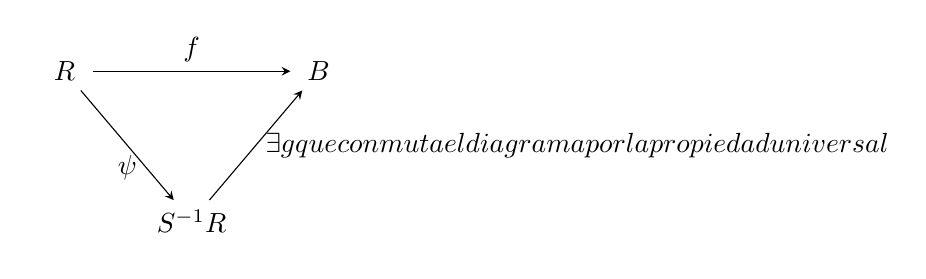
\begin{tikzpicture}
		\matrix (m) [matrix of math nodes,row sep=4em,column sep=2em,minimum width=2em]
		{
			R &  &  B\\
			& S^{-1}R &  \\};
		\path[-stealth]
		(m-1-1) edge node [above] {$f$} (m-1-3)
		(m-1-1) edge node [below] {$\psi$} (m-2-2)
		(m-2-2) edge node [right] {$\exists g \text{ que conmuta el diagrama por la propiedad universal}$} (m-1-3);
		\end{tikzpicture}

		Veamos que ese $g$ es un isomorfismo:
		\begin{itemize}
			\item \textbf{g es sobreyectiva:} Si, por $3)$, todo elemento $a \in B$ es de la forma $f(r)f(s)^{-1}$. Tenemos que ver que para todo elemento de $B$ hay una preimagen en $S^{-1}R$ Basta observar que $g\left( \frac{r}{s} \right) f(r)f(s)^{-1}$.
			\item \textbf{g es inyectiva:} Si porque:
			$$\ker(g) = \{ \frac{r}{s}: g(r)g(s)^{-1}=0_B \} = \{ \frac{r}{s}: f(r)f(s)^{-1}=0_B \} = $$

			Y como $f(s)^{-1}$ es invertible, no es divisor de 0 y por tanto:

			$$ = \{ \frac{r}{s}: f(r)=0_B \} \implies r \in \ker(f) \implies r \in \ker(\psi)\textcolor{red}{???}$$
		\end{itemize}
	\end{proof}

\section{Ideales y localización}

\nota Esto es elemental, pero yo a veces lo dudaba. Sea cualquier función $f: A \longmapsto B$:
\begin{itemize}
	\item Sea un conjunto $M \subset B$, entonces $f(f^{-1}(M)) \subset B$.

	Intuitivamente, al hacer $f^{-1}(M)$ te quedas con los $x \in A$ tal que $f(x) \in M$, pero no todos los $m \in M$ tienen porque tener una preimagen $x \in A$..., por tanto es ahi donde empequeñece el conjunto. Si $f$ es sobreyectiva entonces $f(f^{-1}(M))= B$.
	\item Sea un conjunto $N \subset A$, entonces $f^{-1}(f(N)) \supset A$.

	Intuitivamente, al hacer $f(N)$ te quedas con los $y \in B$ tal que $f(x)=y$, con $x\in N$, pero puede que haya valores de $y$ que sean la imagen de dos valores distintos de $x$, y que alguno de ellos no pertenezca a $N$, es al hacer la preimagen de esos $y$ cuando podemos agrandar el conjunto. Si $f$ es inyectiva entonces $f^{-1}(f(N)) =  A$.
\end{itemize}

Vamos con lo importante, enunciaremos y demostraremos 4 proposiciones sobre ideales y localización. A lo largo de esta sección, consideraremos $\appl{\psi}{R}{S^{-1}R}$ nuestra aplicación de paso al localizado.

En general, si cogemos un ideal $J \subset S^{-1}R$, entonces $\psi^{-1}(J)$ es ideal en $R$. Pero si volvemos a tomar la imagen por ψ no tiene por qué ser un ideal. En secciones anteriores habríamos que podemos considerar el ideal extendido que sí está contenido en $J$: $\psi(\psi^{-1}(J))^e \subset J$. En el caso particular del paso al localizado, tendremos una igualdad.

\begin{prop}
	Sea $\psi:R \longmapsto S^{-1}R$ el homomorfismo de paso al localizado, y sea el ideal $J \subset S^{-1}R$.  Entonces $\psi(\psi^{-1}(J))^e = J$.
\end{prop}

\begin{proof}
	Ya tenemos $\psi(\psi^{-1}(J))^e \subset J$. Por tanto probamos $\psi(\psi^{-1}(J))^e \supset J$:

	Consideramos un elemento $\frac{b}{s} \in J$. Por ser $J$ ideal, tenemos que $\frac{b}{s} \frac{s}{1} = \frac{b}{1} ∈ J$, y su imagen inversa será $b ∈ \inv{ψ}(J)$.

	Ahora simplemente hacemos el camino de vuelta: $ψ(b) = \frac{b}{1} ∈ ψ(\inv{ψ}(J)) ⊂ \psi(\psi^{-1}(J))^e$. Como este último es un ideal, multiplicamos de nuevo $\frac{b}{1}$ por $\frac{1}{s}$ para tener por absorción que $\frac{b}{s} ∈ \psi(\psi^{-1}(J))^e$.
\end{proof}


\obs Todo ideal de $S^{-1}R$ es el extendido de algún ideal de $R$.

Si partimos de un ideal en $R$, también podemos tener un resultado para $\psi^{-1}(\psi(I)^e) $ que contendrá a $I$ (y quizás sea igual a él). Ahora bien, no será tan fácil como el anterior. Vamos a ver primero algunos ejemplos.

\begin{example}
	\begin{itemize}
		\item Sea $\psi: \ent \longmapsto \rac$. $\rac$ es localizado de $\ent$, haciendo invertible $S=\rac \setminus\gen{0}$. Nos queda $\rac=S^{-1}\ent$.

		Si cojo $I=2\ent \implies \psi(I)^e=\rac \implies \psi^{-1}(\psi(I)^e)= \ent$

		\item Sea $S=\{ 2^n \}$, $\psi: \ent \longmapsto \S^{-1}\ent$

		Sea $I=6\ent\implies 6\frac{1}{2}=3 \in \psi(I)^e$... ejemplo sin terminar...
	\end{itemize}
\end{example}

\begin{prop}
	$$\psi^{-1}(\psi(I)^e)=\bigcup_{s\in S}(I:S)$$

	Con $(I:S)=\{ r \in R: r\cdot S \in I \}$.
\end{prop}

\begin{proof}
	\begin{itemize}
		\item $\supset)$ Sea $r \in \bigcup_{s\in S}(I:S) \implies \exists s' \in S$ tal que $r \in (I:s')\implies r\cdot s' \in I \implies \frac{r \cdot s'}{1} \in \psi(I) \textcolor{red}{\implies} \frac{r}{1} \in \psi(I)^e \implies r \in \psi^{-1}(\psi(I)^e)$
		\item $\subset$ Sea $r \in \psi^{-1}(\psi(I)^e)\implies \frac{r}{1}\in \psi(I)^e \implies \frac{r}{1}=\frac{r_1}{s_1}a_1+...+\frac{r_t}{s_t}a_t$ con $a_1,...,a_t \in I \implies s''\frac{r}{a}\in I$ con $s''=s_1...s_t \implies r \in (I:s'')$
	\end{itemize}
\end{proof}

\begin{prop} $\psi^{-1}(\psi(I)^e)=R \Leftrightarrow I \cap S \neq \emptyset$.
\end{prop}

\begin{prop}
	Sea $\pideal \subset R$ un ideal primo, entonces:
	\begin{itemize}
		\item Si $\pideal \cap S \neq \emptyset \implies \psi(\pideal)^e=S^{-1}R$.
		\item Si $\pideal \cap S = \emptyset \implies \psi(\pideal)^e$ es un ideal primo en $S^{-1}R$.
	\end{itemize}
\end{prop}

\begin{proof}
	Vamos a probar que $\psi(\pideal)^e$ es primo.

	Tenemos que $\psi(\pideal)^e\neq \gen{1}$ porque $\pideal \cap S= \emptyset$

	Sean $\frac{r}{s},\frac{r'}{s'} \in S^{-1}R$ tal que $\frac{r}{s}\cdot\frac{r'}{s'} \in \psi(\pideal)^e$.

	Entonces $\frac{r}{s}$ o $\frac{r'}{s'} \in \psi(\pideal)^e \implies \frac{r}{s}\cdot\frac{r'}{s'}=\frac{r_1}{s_1}a_1+...+\frac{r_t}{s_t}a_t$ con $a_1,...,a_t \in \pideal$ y $s_1,...,s_t \in S$.

	Sea $s''=s\cdot s' \cdot s_1 \cdot...\cdot s_t \in S$. Definimos: $\cls{s}=\frac{s''}{s\cdot s'} \in S \subset R$. Entonces:
	$$ \underbrace{\frac{s''}{s\cdot s'}}_{\in S \subset R}\cdot r \cdot r'=\underbrace{s''\frac{r_1}{s_1}a_1+...+s''\frac{r_t}{s_t}a_t}_{\text{comb lineal sobre R de elementos de }\pideal} $$

	Por tanto $(\cls{s})\cdot(r \cdot r') \in \pideal$ que es primo $\implies \underbrace{\cls{s}\in p}_{\textbf{No porque}\pideal \cap S = \emptyset}$ o $r\cdot r' \in \pideal \implies r \cdot r' \in \pideal \implies r$ o $r' \in \pideal$.

	Si $r \in \pideal \implies \frac{r}{1} \in \psi(\pideal)$ y $\frac{r}{s} \in \psi(\pideal)^e$. Si no, de igual modo se prueba que entonces $\frac{r'}{s'}\in \psi(\pideal)^e$.
\end{proof}

Las conclusiones de estas tres proposiciones son \textbf{IMPORTANTES}:
\begin{enumerate}
	\item Todo ideal de $S^{-1}R$ es el extendido de algún ideal de $R$.
	\item Hay una correspondencia biyectiva entre ideales primos $p \subset R$, $p \cap S = \emptyset$ y los ideales primos de $S^{-1}R$.
\end{enumerate}

\notacion
\begin{itemize}
	\item Sea $S \subset R$, $S=\{ a^n \}, a \in R$. Entonces $S^{-1}R=R_a=R_{\{a\}}$. A esto se le llama ``R localizado en a'' o \concept{Localización\IS en un elemento}.
	\item Sea $S=R \setminus \pideal$ con $\pideal \subset R$ ideal primo en $R$. Entonces $S^{-1}R=R_\pideal$. A esto se le llama ``R localizado en el ideal primo $\pideal$'' o \concept{Localización\IS en un ideal primo}, y además $R_\pideal$ es un anillo local.
\end{itemize}


Sea $R=\ent$, no confundir: $\ent_{\{3\}}$, con $\ent_{\gen{3}}$ con $\ent_3$, son todos distintos. Observar que con $R=\ent$ es diferente $R_a$ y $R_{\{a\}}$.
\begin{itemize}
	\item $\ent_{\{3\}}$ es un subanillo de los racionales en el que sólo nos quedamos con aquellos números racionales que admiten una escritura cuyo denominador es una potencia de 3.
	\item $\ent_{\gen{3}}$ es un subanillo de los racionales en el que sólo nos quedamos con aquellos números racionales que admiten una escritura cuyo denominador no es un múltiplo de 3.
	\item $\ent_3=\{ \cls{0},\cls{1},\cls{2} \}$ que no tiene nada que ver con todo esto.
\end{itemize}

\section{Anillos noetherianos}
\begin{defn}[Anillo\IS noetheriano] \label{def:AnilloNoetheriano}
	Se dice que $R$ es un anillo noetheriano si todo ideal $I \subset R$ es finitamente generado (como $R$-módulo). (ver \nref{def:rmodulo_fg})

	%Es decir, que para todo ideal en R  puedo encontrar un número finito de elementos dentro del ideal, de modo tal que cualquier otro elemento que viva en el ideal se puede escribir como combinación lineal de ellos.
\end{defn}

\begin{example}
	\begin{itemize}
	\item $\ent$ es noetheriano, porque es dominio de ideales principales, es decir, todos sus ideales son principales (ver \nlref{def:ideal_principal}).
	\item $K$ cuerpo es noetheriano, porque en un cuerpo solo hay dos ideales, $\{0\}$ y $K$, ambos finitamente generados.
	\item $K[x]$ es noetheriano, porque es dominio de ideales principales.
	\item $K[x_1,...,x_n]$, $\rac[x,y]$ y $\ent[x]$ son noetherianos, pero hay que demostrarlo.
	\item $K[x_1,...,x_n,...]$, con número infinito de variables no es noetheriano.

	Cogemos $I \subset K$, $I= \{ p(\cls{x}): \text{término constante igual a 0} \}$.

	\notacion $\cls{x}=\{x_1,x_2,...,x_n,...\}$
	\nota En $I$ no existe el polinomio $p(\cls{x})=x_1+x_2+...+x_n+...$ ya que no se pueden sumar un número infinito de sumandos. Las combinaciones lineales finitas sí están.

	Entonces tenemos que $I$ es un ideal (cumple las tres condiciones de los ideales), y que $p(\cls{x})=x_i \in I$ $ \forall i$. Pero $I$ no es finitamente generado.
	\begin{proof}
		Supongamos que $\exists p_1,...,p_s \in K[x_1,...,x_n,...]$ tal que $I=\gen{p_1,...,p_s}$, tal que $p_1,...,p_s$ solo dependen de un número finito de variables.

		Supongamos sin pérdida de generalidad que sólo dependen de $x_1,...,x_n$.

		Entonces es imposible escribir $x_{n+1}$ como combinación de los $p_i$. $x_{n+1}\neq q_1p_1+...+q_sp_s$, como mucho obtenemos productos $x_ix_{n+1}$, pero nunca $x_{n+1}$ solo.
	\end{proof}
	\end{itemize}
\end{example}

\begin{prop}\label{prop:caracterizacion_noetheriano}
	Son equivalentes:
	\begin{enumerate}
		\item $R$ es noetheriano.
		\item Toda cadena creciente de ideales en $R$, $\{I_i\}_{i \in \nat}$ estabiliza para un $n$ suficientemente grande: $I_1 \subseteq I_2 \subseteq ... \subseteq I_n = I_{n+1}$.
		\item Todo conjunto no vacío de ideales en $R$ tiene un elemento maximal (No tiene por qué ser un ideal maximal).
	\end{enumerate}
\end{prop}

\begin{proof}

		\proofpart{$1) \implies 2)$}

		Sea $R$ un anillo noetheriano y sea $\{I_i\}_{i \in \nat}$ una cadena creciente de ideales en $R$. Queremos probar que la cadena estabiliza para algún $N$ suficientemente grande.

		Sea $J= \bigcup_{i \in \nat} I_i$. Entonces $J$  es un ideal en $R$. En general la union de ideales no tiene porque ser un ideal, pero en el caso de ser una cadena creciente sí lo es (mirar demostración del teorema \ref{thm:IdealContenidoMaximal}). Como $R$ es noetheriano, $J$ es finitamente generado, por tanto existen $a_1,...,a_s \in J$ tal que $J=\gen{a_1,...,a_s}$.

		Además tenemos que $I_1 \subseteq I_2 \subseteq ... \subseteq I_N \subseteq ...$, por tanto, $\exists k$ tal que  $a_1,...,a_s \in I_k = J = \gen{a_1,...,a_s}$

		\proofpart{$2) \implies 3)$}

		Sea $\Sigma$ un conjunto no vacío de ideales en $R$, queremos probar que tiene un elemento maximal.

		Supongamos que en $\Sigma$ hay una cadena creciente de ideales $\{I_i\}$. Por la hipótesis en $2)$, la cadena estabiliza, luego tiene un elemento maximal.

		Si esa cadena no existe, se construye. Tenemos un conjunto de ideales $\set{I_i}$, así que construimos la cadena $I_1 ⊆ I_1 ∪ I_2 ⊆ I_1 ∪ I_2 ∪ I_3 ⊆ \dotsb$ y aplicamos lo de antes\footnoteby{Guille}{No tengo claro qué hacer si el conjunto de ideales es no numerable. Ahora bien, parece que ese no es un caso que estemos considerando en ningún momento.}.

		\proofpart{$3) \implies 1)$}

		Sabemos que todo conjunto no vacío de ideales en $R$ tiene un elemento maximal, y queremos probar que $R$ es noetheriano.

		Sea $I \subset R$, supongamos que $I\neq \{0\}$ y que $I$ no es finitamente generado.
		\begin{itemize}
			\item Sea $a_1 \in I, a_1 \neq 0$.
			\item Sea $a_2 \in I\setminus \gen{a_1}$. Puedo encontrar ese $a_2$ porque si no lo encontrara querría decir que $I$ sería finitamente generado.
			\item Sea $a_3 \in I\setminus \gen{a_1,a_2}$.
			\item Sea $a_n \in I\setminus \gen{a_1,...,a_n}$.
		\end{itemize}
		Considero $\gen{a_1}\subsetneq \gen{a1,a2} \subsetneq \gen{a_1,a_2,a_3} \subsetneq...$. Esta cadena creciente de ideales nunca estabiliza. Lo cual es contradictorio porque entonces podría haber definido $\Sigma=\{ \gen{a_1}, \gen{a_1},\gen{a_1,a_2},...,\gen{a_1,a_2,...,a_n},.... \} \neq \emptyset$ y no tiene elemento maximal.
\end{proof}

\begin{theorem}[Teorema\IS de la base de Hilbert]\label{thm:tma_base_hilbert}
	Sea $R$ un anillo noetheriano. Entonces $R[x]$ es un anillo noetheriano.
\end{theorem}

\begin{proof}
	Sea $I \subset R[x]$, queremos probar que $I$ es finitamente generado.
	\nota El coeficiente director de un polinomio es el coeficiente que acompaña al término de mayor grado.
	\nota El grado es un numero $a \in \nat$, y los $\nat$ son ordenables, por tanto, si hablamos de grado mínimo, que no nos extrañe, es lo que todos pensamos: el grado menor.

	Vamos a suponer que $I$ no es finitamente generado, podemos suponer que $I\neq \{0\}$, así:
	\begin{itemize}
		\item Sea $f_1(x) \in I$ con grado mínimo, sea $a_1$ el coeficiente director de $f_1(x)$.
		\item Sea $f_2(x) \in I\setminus \gen{f_1(x)}$ con grado mínimo, puedo cogerlo ya que hemos supuesto que $I$ no es finitamente generado, sea $a_2$ el coeficiente director de $f_2(x)$.
		\item Sea $f_{k+1}(x) \in I\setminus \gen{f_1(x),...,f_k(x)}$ con grado mínimo, sea $a_{k+1}$ el coeficiente director de $f_k(x)$.
	\end{itemize}

	Entonces, con los coeficientes directores puedo montar la siguiente cadena: $\gen{a_1} \subseteq \gen{a_1,a_2} \subseteq ... \subseteq \gen{a_1,...,a_k,a_{k+1}}$, que es una cadena creciente de ideales de $R$, además sabemos por hipótesis que $R$ es noetheriano, por tanto esa cadena se debe estabilizar.

	Pero hemos supuesto que $I$ no es finitamente generado, y afirmamos que si eso ocurre, la cadena anterior no puede estabilizar, vamos a probar eso:

	Supongamos que estabiliza $\implies$ para algún $k$ se cumple que $\gen{a_1,...,a_k}=\gen{a_1,...,a_k,a_{k+1}} \implies \exists b_1,...,b_k \in R$ tal que: $a_{k+1}=b_1a_1+...+b_ka_k$. Donde $a_{k+1}$ es el coeficiente director de $f_{k+1}(x)$. Defino:

	\textcolor{red}{Revisar el final de esta demostracion}

	$$ g=f_{k+1}(x)-\sum_{i=1}^{k}b_ix^{\deg(f_{k+1}(x))-\deg(f_i(x))} f_i(x) \in I\setminus \gen{f_1,...,f_k} $$

	%Como las $f_i$ tiene grado igual o mayor, estoy haciendo es obtener justamente el a_{k+1} con signo negativo.

	Tenemos que $\deg(g) < \deg(f_{k+1}(x))$. Lo cual es contradictorio porque $g \in I \setminus \gen{f_1,...,f_k}$ y tiene grado < $\deg(f_{k+1})$.

\end{proof}

\begin{example}
	\begin{itemize}
	\item $\ent[x_1,...,x_n]$ es noetheriano. No hay más que coger $\ent$, que sabemos que es noetheriano, y 'aplicar' el teorema anterior n veces.
	\item $\K[x_1,...,x_n]$ es noetheriano por el mismo motivo.
	\item Si $R$ es noetheriano $\implies$ $R[x_1,...,x_n]$ es noetheriano.
	\end{itemize}
\end{example}

\subsection{Anillos noetherianos y paso al cociente}

\begin{prop} \label{prop:NoetherianoCociente}
	Sea $R$ un anillo noetheriano y sea $I \subset R$ un ideal $\implies$ $\quot{R}{I}$ también es noetheriano.
\end{prop}
\begin{proof}
	Sea $\pi: R \longmapsto \quot{R}{I}$, tenemos que probar que $J \subset \quot{R}{I}$ es finitamente generado.

	Cogemos $L \subset R$ ideal de $R$ tal que $I \subset L$ y tal que $\pi(L)=J$ ($L$ es posible de encontrar, ver \ref{relacionRconRI}, relación entre los ideales de $R$ y $\quot{R}{I}$, apartado 2). Como $R$ es noetheriano, $L$ es finitamente generado, es decir, $\exists a_1,...,a_s \in L$ tal que $L=\gen{a_1,...,a_s} \implies J=\gen{\pi(a_1),...,\pi(a_s)}$.

	También se puede probar utilizando la segunda caracterización de los anillos noetherianos (ver proposición \ref{prop:caracterizacion_noetheriano}). Cualquier cadena creciente de ideales en $R$ estabiliza, si me fijo en una cadena creciente de ideales en $\quot{R}{I}$, viene de una cadena creciente de ideales en $R$, por la correspondencia biyectiva.
\end{proof}

Una consecuencia de lo anterior es:

\obs Sea $R$ un anillo noetheriano y sea $T$ una $R$-álgebra de tipo finito (ver definición de $R$-álgebra finitamente generada: \ref{def:ralgebra_fg}). Entonces $T=R[b_1,...,b_n]$ para ciertos $b_1,...,b_n \in T$. De hecho $T=R[b_1,...,b_n]$ es también noetheriano.

\begin{proof}
	Sea $R$ un anillo noetheriano, le añadimos n variables (sigue siendo noetheriano por el teorema de Hilbert \ref{thm:tma_base_hilbert}) y definimos el siguiente homomorfismo de $R$-álgebras:

	\begin{align*}
		\psi: R[x_1,...,x_n] & \longmapsto  T=R[b_1,...,b_n]\\
		r \in R & \longmapsto r \\
		x_i & \longmapsto b_i \\
	\end{align*}

	Entonces $\psi$ es un homomorfismo de $R$-álgebras y es sobreyectivo por cómo lo hemos construido. Ahora aplicamos el primer teorema de isomorfía:
	$$ \quot{R[x_1,...,x_n]}{\ker(\psi)} \simeq \img(\psi)=T=R[b_1,...,b_n]$$

	Por tanto tenemos:
	 $$\quot{\text{anillo noetheriano}}{\text{ideal}}$$

	Y como hemos visto antes, eso es noetheriano. Por tanto: $T=R[b_1,...,b_n]$ es noetheriano.
\end{proof}

\begin{example}
	\begin{itemize}
		\item $\rac[\sqrt{2},x, \pi]$ es una $\rac$-álgebra.
		\item $\real$ es una $\rac$-álgebra pero no de tipo finito.
	\end{itemize}
\end{example}

\subsection{Anillos noetherianos y localización}

\begin{prop} \label{prop:NoetherianoLocalizacion}
	Sea R un anillo noetheriano y sea $S\subset R$ una parte multiplicativa. Construimos como otras veces el siguiente homomorfismo:
	$$\psi: R \longmapsto S^{-1}R$$

	Entonces $S^{-1}R$ es noetheriano.
\end{prop}
\begin{proof}
	Para ello tenemos que probar que sea $J \subset S^{-1}R$ un ideal, este es finitamente generado.

	Lo cual es cierto ya que $J$ es el extendido de algún ideal de $R$ y hemos probado que $\psi(\psi^{-1}(J))^e=J$. Por tanto $J$ es el extendido de $\psi^{-1}(J)\subset R \implies J$ es finitamente generado. \textcolor{red}{Revisar cuando repase lo que dimos esos días...} %min 19
\end{proof}



% -*- root: ../AlgebraConmutativa.tex -*-
\chapter{Variedades algebraicas afines}
El objetivo de este tema es hacer geometría usando el Álgebra Conmutativa. Para ellos vamos a disponer de un 'campo de juego' y de unas 'herramientas':

\begin{center}
	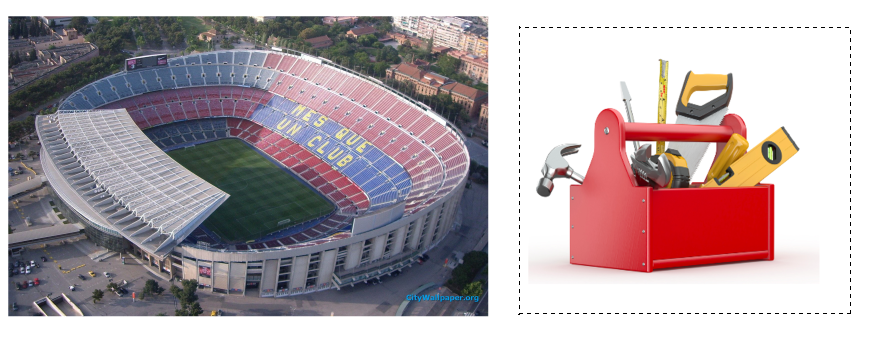
\includegraphics[scale=0.45]{img/vaa.png}
\end{center}

\begin{itemize}
	\item Nuestro 'campo de juego' no será tan increíble, exitoso y espectacular como el que aparece en la imagen. Será $\A^n_K$, o también llamado espacio afín de dimensión $n$ sobre un cuerpo $\K$ (tuplas sobre un cuerpo $\K$). Como un ejemplo vale más que x palabras con x tendiendo a 100, os pongo uno: $\A^2_{\real}$ es el plano, y las tuplas son los puntos $(x,y)$ del plano.
	\item Las herramientas serán lo que hemos dado hasta ahora, anillos noetherianos, dominios de integración, dominios de factorización única... Que empiece el juego.
\end{itemize}

\begin{defn}[Variedad algebraica]\label{def:variedad_algebraica}
	Diremos que un subconjunto $X\subset \A^n_K$ es una variedad algebraica afín si los puntos de $X$ son las soluciones de alguna colección $F$ de polinomios en $\K[x_1,...,x_n]$. 
	
	Es decir, $X$ es una variedad algebraica afín (v.a.a.) si existe $F \subset K[x_1,...,x_n]$ tal que $X=\{ (a_1,...,a_n) \in \A_K^n: p(a_1,...,a_n)=0,  \forall p(x_1,...,x_n) \in F \} = \V(F)=\text{ 'Conjunto de soluciones de F '}$. 
\end{defn}

En resumen, a grandes rasgos y para entendernos tenemos que:
\begin{itemize}
	\item Una variedad algebraica no es más que un conjunto de puntos que son solución de unas ecuaciones dadas.
	\item Dada una variedad algebraica, existe un conjunto de ecuaciones que tienen por solución los puntos pertenecientes a dicha variedad algebraica.
\end{itemize}

Vemos algunos ejemplos de variedades algebraicas afines.
\begin{example}
	\begin{itemize}
		\item $\emptyset = \V(1)$. La ecuación $1=0$ no tiene solución. $\emptyset$ siempre es una v.a.a.
		\item $\A_K^n=\V(0)$. Todos los puntos del espacio afín son solución de la ecuación $0=0$. $\A_K^n$ siempre es una v.a.a.
		\item Ahora cogemos $A^1_k$, que es la recta afín sobre un cuerpo K (por ejemplo si el cuerpo fuera $\real$, este espacio afín serían todos los puntos de $\real^1$).
		
		Si cojo $F=\{p(x)\}$, la variedad algebraica afín serán los puntos que son solución de la ecuación $p(x)=0$. Es decir, $\V(F)$ puede ser $\emptyset$ o un número finito de puntos, como mucho tantos como el grado de $p(x)$.
		\item Ahora vamos a coger una variedad afín y vamos a encontrar $F$. Es decir, cogemos un conjunto de puntos y buscamos qué ecuaciones son soluciones de todos a la vez.
		
		Por ejemplo: Sea $\K=\real$, $\{1,2,3\} =\V((x-1)(x-2)(x-3))$. Que no es lo mismo que: $\V(x-1,x-2,x-3)=\emptyset$, ya que no hay ningún valor $x$ tal que esas 3 ecuaciones sean 0 a la vez. 
		
		De hecho la variedad algebraica anterior es más grande que lo que hemos dicho, sería: $\{1,2,3\} =\V(\gen{(x-1)(x-2)(x-3)})$. Recordemos que $\gen{(x-1)(x-2)(x-3)} = \{ p(x)(x-1)(x-2)(x-3) : p(x) \in \real[x] \}$ (todos los múltiplos de $(x-1)(x-2)(x-3)$)
	\end{itemize}
\end{example}

\obs Todo conjunto finito de puntos en $\A_K^n$ es una variedad algebraica.

\obs Sea $Y$ una colección infinita de puntos en $A^1_n$ (distinta del total), entonces $Y$ NO es una variedad algebraica afín. Ya que el conjunto de soluciones de $p(x)=0$ está acotado por el grado de $p(x)$, así que salvo que $Y=\A^n_k$, $Y$ no puede ser una v.a.a.

Así, sin mucho esfuerzo hemos descrito todas las variedades afines de la recta, que son el vacío, el total, y conjuntos finitos de puntos.

Ahora vamos a pensar en  $\A_K^2$:
\begin{example}	
	Sea $\A_K^2$, entonces tenemos $K[x_1,x_2]$. Vamos a buscar $F$ para:
	
	\begin{enumerate}
		\item $(a_1,a_2) \in \A^2_k$.
		
		Probamos con $F=\{(x_1-a_1)(x_2-a_2)\}$. Que no es lo que buscamos ya que $(x_1-a_1)(x_2-a_2)=0$ tiene por solución dos rectas (las de color azul):
		
		\begin{center}
			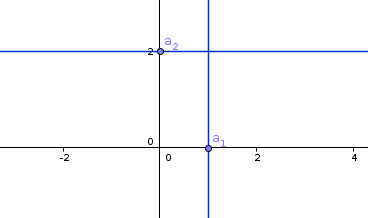
\includegraphics[scale=0.45]{img/ej1.png}
		\end{center}
		
		La solución buena es:  $F=\{(x_1-a_1),(x_2-a_2)\}$ ya que el sistema de ecuaciones $(x_1-a_1)=0$ y $(x_2-a_2)=0$ tiene como solución el punto de intersección de ambas rectas que es precisamente $(a_1,a_2)$.
		
		\begin{center}
			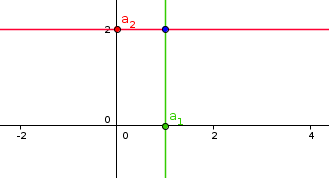
\includegraphics[scale=0.45]{img/ej2.png}
		\end{center}
		
		
		\item $(a_1,a_2),(b_1,b_2) \in \A^2_k$. Buscamos $F$
		
		Se nos ocurre probar con:
		\[
		\left.
		\begin{array}{rcl}
		(x_1-a_1)(x_2-b_2) & = & 0  \text{ \textcolor{green}{-----}}\\
		(x_2-a_2)(x_1-b_1) & = & 0 \text{ \textcolor{red}{-----}}
		\end{array}
		\right\}
		\]
		
		\begin{center}
			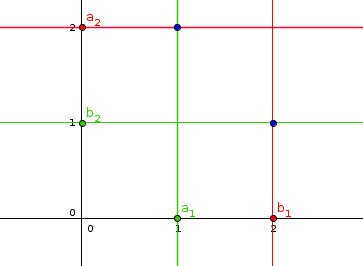
\includegraphics[scale=0.45]{img/ej3.png}
		\end{center}
		
		Que vale como solución salvo si $b_2=a_2$ o $a_1=b_1$ en cuyo caso nos saldría una recta como solución, que difiere de lo que buscamos que son dos puntos.
		
		La solución buena es:
		\[
		\left.
		\begin{array}{rcl}
		(x_1-a_1)(x_2-b_2) & = & 0 \text{ \textcolor{green}{-----}}\\
		(x_2-a_2)(x_1-b_1) & = & 0 \text{ \textcolor{red}{-----}}\\
		(x_1-a_1)(x_1-b_1) & = & 0 \text{ \textcolor{black}{-----}}\\
		(x_2-a_2)(x_2-b_2) & = & 0 \text{ \textcolor{purple}{-----}}
		\end{array}
		\right\}
		\]
		
		Que gráficamente es superponer el dibujo anterior con este:
		
		\begin{center}
			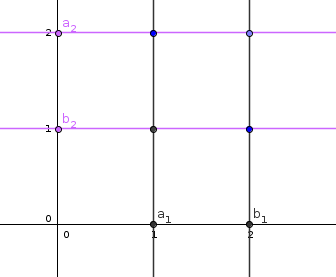
\includegraphics[scale=0.45]{img/ej4.png}
		\end{center}
		
		Por tanto $F=\{ (x_1-a_1)(x_2-b_2), (x_2-a_2)(x_1-b_1), (x_1-a_1)(x_1-b_1), (x_2-a_2)(x_2-b_2)  \}$
	\end{enumerate}
\end{example}


\begin{prop}
	Sea $F \subset \K[x_1,...,x_n]$ no vacío. Entonces $\V(F)=\V(\gen{F})$.
\end{prop} 

\begin{proof}
	\begin{itemize}
		\item $F \subseteq \gen{F} \implies \V(F) \supset \V(\gen{F})$. Es obvio, ya que en $\gen{F}$ hay más ecuaciones que cumplir que en $F$.
		\item Vamos a ver la otra inclusión: $\V(F) \supset \V(\gen{F})$.
		
		Sea $(a_1,...,a_n) \in \V(F) \implies \forall p(x_1,..,x_n) \in F$, $p(a_1,...,a_n)=0$. Y para que $(a_1,...,a_n) \in \V(\gen{F})$ tenemos que ver que $\forall q(x_1,...,x_n)\in \gen{F}$, $q(a_1,...,a_n)=0$.
		
		Si $q(x_1,...,x_n)\in \gen{F} \implies \exists c_1(x_1,...,x_n),...,c_s(x_1,...,x_n) \in F$ y $\exists b_1(x_1,...,x_n),...,b_s(x_1,...,x_n) \in \K[x_1,..,x_n]$ tal que $q(x_1,...,x_n)=b_1c_1+...+b_sc_s$.
		
		Entonces $q(a_1,...,a_n)=b_1(a_1,...,a_n)c_1(a_1,...,a_n)+...+b_s(a_1,...,a_n)c_s(a_1,...,a_n) = 0$  ya que $c_i=0$.
	\end{itemize}
	
	Nos falta el caso de que $\V(F)=\emptyset$. Pero el $\emptyset$ está contenido en cualquier conjunto.
\end{proof}

Pero... ¿por qué es interesante que $\V(F)=\V(\gen{F}$?

Como $\gen{F}\subset \K[x_1,...,x_n] \implies \gen{F}$ es finitamente generado, es decir, existe $p_1(x_1,...,x_n),...,p_t(x_1,...,x_n)$ tal que $\gen{F} = \gen{p-1(x_1,...,x_n),...,p_t(x_1,...,x_n)} \implies \V(F)=\V(\gen{F})=\V(p_1(x_1,...,x_n),...,p_t(x_1,...,x_n))$:

\obs Toda v.a.a. es el conjunto de solución de un nº finito de ecuaciones polinómicas.

\section{Topología de Zanski en \Akn}
Sea $\Akn$, entonces tanto $\emptyset$ como $\Akn$ son v.a.a., además $\emptyset=\V(\gen{1})$ y $\Akn=\V(0)$.


\begin{itemize}
	\item Sean $X_1$ y $X_2$ dos v.a.a. $\implies$ $X_1 \cap X_2$ es v.a.a..
	
	Esto es cierto ya que $X_1=\V(I_1)$ y $X_2=\V(I_2)$ para $I_1,I_2$ ideales en $\K[x_1,...,x_n] \implies$ 
	$$X_1 \cap X_2 = \V(I_1 \cup I_2)=\V(I_1+I_2)$$
	
	\textcolor{red}{$X_1$ y $X_2$ son ideales porque hemos visto que $\V(F)=\V(\gen{F})$, y $K[x_1,..,x_n]$ es noetheriano y por tanto cualquier ideal es finitamente generado}
	
	Conclusiones:
	\begin{enumerate}
		\item La intersección de un número finito de v.a.a. es una v.a.a.
		\item La intersección infinita de v.a.a. también es v.a.a.: Sea $\{ X_i \}_{i\in I}$ una colección de v.a.a., entonces:
		\[ \cap_{i\in I}X_i = \V(\gen{I_i, i \in I}) \]
	\end{enumerate}
	\item Sean $X_1, X_2$ dos v.a.a. $\implies X_1 \cup X_2$ es v.a.a..
	
	De hecho sea  $X_1=\V(I_1)$ y $X_2=\V(I_2)$,  para $I_1=\gen{f_1,...,f_s},I_2=\gen{g_1,...,g_t}$ ideales en $\K[x_1,...,x_n]$ entonces 
	$$X_1 \cup X_2=\V(I_1 \cap I_2)=\V(I_1 \cdot I_2)=\gen{f_i, g_j}$$
	
	Conclusiones
	\begin{enumerate}
		\item La unión de un número finito de v.a.a. es una v.a.a.
		\item La unión arbitraria infinita de v.a.a. no tiene porque ser v.a.a. (Todos los enteros de $\ent$ no son v.a.a.)
	\end{enumerate}
\end{itemize}

Todo esto que hemos visto son una serie de conjeturas que son ciertas pero que aún no vamos a demostrar.

Nos quedamos con la siguiente proposición: 

\begin{prop}
	Las variedades algebraicas afines satisfacen los axiomas de los cerrados de una topología. En $\Akn$ definimos la topología de Zanski, como aquella en la que los cerrados son variedades algebraicas afines.
\end{prop} 

\begin{example}
	Topología de Zanski en $\A^1_K$:
	\begin{itemize}
		\item Cerrados: $\emptyset$, $\A^1_K$ y $\{ p_1,...,p_n \} \subset \A^1_K$ (cantidad finita de puntos).
		\item Abiertos: (los complementarios de los cerrados) $\A^1_K$, $\emptyset$, y el complementario de una cantidad finita de puntos.
	\end{itemize}
\end{example}



% Clase 7/3/2016
Vamos a ver algunas propiedades de estas variedades generadas por ideales. Por ejemplo, si tomamos dos ideales $J, I ⊂ K[x_1, \dotsc, x_n]$, si $J ⊂ I$ entonces $\V(J) ⊃ \V(I)$.

Los radicales también nos darán resultados interesantes. A priori, un radical nos debería dar una variedad más pequeña al ser un ideal más grande. La cuestión es que lo que nos dará en realidad será la misma variedad.

\begin{prop} Sea $I ⊂ K[x_1, \dotsc, x_n]$ un ideal, y consideramos su radical $\sqrt{I}$. Entonces $\V(I) = \V(\sqrt{I})$.
\end{prop}

\begin{proof}

\proofpart{$⊃$}

Como $I ⊂ \sqrt{I}$, es obvio que $\V(I) ⊃ \V(\sqrt{I})$.

\proofpart{$⊂$}

Lo primero que tenemos que hacer es tener cuidado cuando el ideal es el vacío. Ahora bien, si $\V(I) = ∅$, entonces $\V(\sqrt{I}) = ∅$ igualmente, ya que hemos demostrado antes que $\V(\sqrt{I}) ⊂ \V(I)$.

Podemos suponer entonces que $\V(I) ≠ ∅$. Sea $(a_1, \dotsc, a_n) ∈ \V(I)$ o, en otras palabras, que $∀p(x_1, \dotsc, x_n) ∈ I$ se tiene que $p(a_1, \dotsc, a_n) = 0$.

Queremos demostrar que $(a_1, \dotsc, a_n) ∈ \V(\sqrt{I})$ y por lo tanto que $∀q(x_1, \dotsc, x_n) ∈ \sqrt{I}$ tengamos que $q(a_1, \dotsc, a_n) = 0$. Ahora bien, por ser $q$ elemento del radical, elevado a una potencia $m > 0$ nos dará cero, luego en particular $q(a_1, \dotsc, a_n)^m = 0$. Pero $q(a_1, \dotsc, a_n) ∈ K$ que es un cuerpo y dominio de integridad, así que si elevado a una potencia nos da $0$ tiene que ser él mismo cero, y por lo tanto $(a_1, \dotsc, a_n) ∈ \V(\sqrt{I})$.
\end{proof}

\subsection{La operación $\I(S)$}

Vamos a tomar un subconjunto $S ⊂ \A_K^n$. Nos fijaremos en todos los polinomios en $n$ variables que se anulan en $S$. Es decir, \[ \I(S) = \set{p(x_1, \dotsc, x_n) ∈ K[x_1, \dotsc, x_n] \tq ∀(a_1, \dotsc, a_n) ∈ S \; p(a_1, \dotsc, a_n) = 0} \]

No es difícil ver que $\I(S)$ es un ideal: no es vacío ($0 ∈ \I(S)$), está cerrado con la suma y la propiedad de absorción también se cumple trivialmente.

\begin{wrapfigure}{R}{0.4\textwidth}
\centering
\begin{tikzpicture}
\draw[->] (-0.5, 0) -- (3,0);
\draw[->] (0, -0.5) -- (0,2);

\draw[|-|, very thick, blue] (0,0) node[anchor = north west, yshift = -0.05cm, xshift = -0.05cm] {$0$} -- (1,0) node[below, yshift = -0.05cm] {$1$};
\end{tikzpicture}
\caption{El intervalo $[0,1]$ no es una variedad algebraica.}
\label{fig:Interv01}
\end{wrapfigure}

Por ejemplo, podemos buscar todos los polinomios que se anulan en el intervalo $S= [0,1]$. Está claro que $\gen{y} = \I(S)$, pero no vamos a poder encontrar un polinomio que se anule sólo en $S$. La razón es que $S = [0,1]$ no es una variedad algebraica. Esto nos va a dar un lema interesante.

\begin{lemma} Sea $S ⊂ \A_K^n$ un subconjunto del espacio afín. Entonces $\V(\I(S)) ⊃ S$, y la igualdad $\V(\I(S)) = S$ se da si y sólo si $S$ es una variedad algebraica afín.
\end{lemma}

\begin{proof} Por definición, siempre tenemos que $S ⊂ \V(\I(S))$. Supongamos que $S = \V(\I(S))$. Es claro que $S$ es una variedad algebraica afín, porque la igualdad indica que $S$ es el conjunto de ceros del ideal $\I(S)$.

Vamos a ir con la demostración al otro lado. Supongamos que $S$ es una variedad algebraica afín, y queremos demostrar que $S = \V(\I(S))$.

Como $S$ es una v.a.a., entonces $∃ J ⊂ K[x_1, \dotsc, x_n]$ tal que $S = \V(J)$, luego $J ⊂ \I(S)$. Entonces podemos hacer una cadena \[ S = \V(J) ⊃ \V(\I(S)) ⊃ S \], por lo que todas las inclusiones tienen que ser igualdades.
\end{proof}

Este lema lo podemos relacionar con la topología de Zariski que veíamos antes, que nos decía que los cerrados eran las variedades algebraicas.

\begin{corol} Sea $S ⊂ \A_K^n$. Entonces la \concept{Clausura\IS de Zariski} de $S$ es $\adh{S} = \V(\I(S))$, y entonces $\adh{S}$ es la variedad algebraica más pequeña que contiene a $S$.
\end{corol}

\begin{proof}
Sabemos que $S ⊂ \V(\I(S))$, donde $\V(\I(S))$ es una variedad algebraica afín. Tenemos que probar que además es la variedad más pequeña que contiene a $S$.

Hacemos la demostración por reducción al absurdo, suponiendo que existe una variedad algebraica afín $X ⊃ S$ y además $X \subsetneq \V(\I(S))$. Ahora bien, es obvio que $\I(S) ⊃ \I(X) ⊃ \I(\V(\I(S)))$. Podemos volver a tomar la variedad y entonces \[ \V(\I(S)) ⊂ \underbracket{\V(\I(X))}_{ = X} ⊂ \underbracket{\V(\I(\V(\I(S))))}_{= \V(\I(S)))} \], luego $X = \V(\I(S))$, contradicción.
\end{proof}

Dos observaciones:

\begin{prop}
Dado $S ⊂ \A_K^n$, el ideal $\I(S)$ es un ideal radical.
\end{prop}

\begin{proof} Ejercicio para el lector.
\end{proof}

\begin{prop} Sea $X ⊂ \afesp$ una variedad algebraica afín. Entonces existe $J ⊂ K[x_1, \dotsc, x_n]$ tal que $\V(J) = X$.
\end{prop}

El ideal $J$ no es el único que determina a $X$. Sin embargo, el ideal $\I(X)$ es el ideal más grande de $K[x_1, \dotsc, x_n]$ cuyos ceros son $X$, esto es, es el ideal más grande tal que $X = \V(\I(X))$.

Esto nos permite asociar un ideal radical a $X$ sin ninguna ambigüedad. Diremos entonces que $I(X)$ es el ideal que determina a $X$.

% -*- root: ../AlgebraConmutativa.tex -*-
\chapter{Teorema de los ceros de Hilbert}

Hemos jugado en $\Akn$ y en $\K[x_1,\dotsc,x_n]$. Y sabemos movernos de un sitio a otro:

\begin{align*}
	\Akn & \longmapsto  \K[x_1,...,x_N] \\
	X & \longmapsto  \I(X) \\
	\V(J) & \leftarrow  J \\
\end{align*}

\begin{itemize}
	\item Del lado izquierdo me interesan las v.a.a., si cojo $X\in \Akn$ v.a.a., puedo ir a $\I(X) \in \K[x_1,...,x_n]$ y volver a $\V(\I(X)) \in \Akn$ que es igual a $X$ por ser una v.a.a..

	\item Del lado derecho, me interesan los ideales, porque determinan v.a.a., pero me basta quedarme con los ideales radicales ya que genera la misma v.a.a. un ideal $I$ y su $Rad(I)$. 
	
	Sin embargo, no ocurre como antes en cuanto a que si cojo $J$ ideal radical en $\K[x_1,...,x_n]$, puedo ir a $\V(J)$ en $\Akn$, y volver a $\I(\V(J)) \supseteq J$. Pero puede pasar que la inclusión sea estricta:
	\begin{example}
		\begin{enumerate}
			\item Ejemplo de inclusión estricta:
			\begin{align*}
				\A^1_{\real} & \longmapsto  \real[x] \\
				\V(\gen{x^2+1}) & \leftarrow  \gen{x^2+1} \\
				\shortparallel & \\
				\emptyset & \longmapsto  \I(\{ \emptyset \})=\real[x] \\
			\end{align*}
			\item Otro ejemplo de inclusión estricta:

			Cogemos en $\real[x,y]$ e ideal  radical $\gen{(x-1)^2+(y-2)^2}$, que es primo (y por tanto radical) porque $p(x,y)=(x-1)^2+(y-2)^2$ es irreducible en $\real[x,y]$.

			Esto es así porque $\real[x,y] \subset \cplex[x,y]$  que es un dominio de factorización única.

			Y en $\cplex[x,y]$ tenemos que $p(x,y)=(x-1)^2+(y-2)^2=((x-1)+i(y-2))((x-1)-i(y-2))$. Por tanto no se puede factorizar de otra forma.

			\begin{align*}
				\A^2_{\real} & \longmapsto  \real[x,y] \\
				\V(J) & \leftarrow  \gen{(x-1)^2+(y-2)^2}=J \\
				\shortparallel & \\
				X=\{1,2\} & \longmapsto  \I(X)=\gen{x-1,y-2}\\
			\end{align*}

			Y obviamente $\gen{(x-1)^2+(y-2)^2} \subsetneqq \gen{x-1,y-2}$
		\end{enumerate}
	\end{example}
\end{itemize}

\textbf{Conclusión:} Ideales radicales \textbf{distintos} determinan variedades algebraicas iguales, esto nos molesta, porque no hay una relación 1 a 1 entre ideales radicales y v.a.a.. No hay un diccionario entre v.a.a. en $\Akn$ e ideales radicales en $\K[x_1,...,x_n]$.

Y aquí empieza la motivación de este tema, en buscar algo que nos permita tener ese diccionario, y eso lo conseguimos gracias a Hilbert!!

\begin{theorem}[Teorema de los ceros de Hilbert]\label{teor:tma_0_hilbert}
	Si $\K$ es algebraicamente cerrado y $J \subset K[x_1,...,x_n]$ es radical, entonces $J=\I(\V(J))$
\end{theorem}



\textbf{Corolario:}	Si $\K$ es algebraicamente cerrado, hay una correspondencia biyectiva entre variedades algebraicas afines en $\Akn$ e ideales radicales en $\K[x_1,...,x_n]$

Nuestro objetivo en este tema es probar el teorema de los ceros de Hilbert \ref{teor:tma_0_hilbert}. Para ello, vamos a utilizar algunas proposiciones y teoremas:

\begin{theorem}[Teorema básico]
	Sea $\K$ un cuerpo algebraicamente cerrado, entonces todo ideal maximal en $\K[x_1,...,x_n]$ es de la forma $\gen{x_1-a_1,...,x_n-a_n}$ con $a_1,...,a_n \in \K$
\end{theorem}

\obs En $\K[x_1,...,x_n]$ todo ideal de la forma $\gen{x_1-a_1,...,x_n-a_n}$ es maximal aunque $\K$ no sea algebraicamente cerrado ya que:
$$ \quot{\K[x_1,...,x_n]}{\gen{x_1-a_1,...,x_n-a_n}} \simeq \K $$

\obs Supongamos $\rac = \K$. Tomamos $\rac[x,y]$, entonces $\gen{x-1,y^2-2}$ es maximal ya que $\quot{\rac[x,y]}{\gen{x-1,y^2-2}} \simeq \rac(\sqrt{2})$  que es un cuerpo.

Pasa lo mismo con $\gen{x-1,y^7+3y^2+3}$ o con $\gen{x^5+5x+5, y^7+3y^2+3}$. \textcolor{red}{wtf son estos ejemplos, luego dice algo así como que salen extensiones finitas de grado el producto}

\begin{theorem}[Teorema débil]
	Sea $\K$ un cuerpo algebraicamente cerrado y sea $I$ un ideal propio $\subsetneqq \K[x_1,...,x_n]$. Entonces $\V(I) \neq \emptyset$.
\end{theorem}

\obs Si tomamos un cuerpo que no es algebraicamente cerrado esto no tiene porque pasar, por ejemplo en $\real[x]$ el conjunto $\V(\gen{x^2+5})=\emptyset$


Demostramos el teorema débil:
\begin{proof}
	Sea $I \subsetneqq \K[x_1,...,x_n] \implies \exists M$ maximal en $\K[x_1,...,x_n]$ tal que $I \subset M$. Por el teorema básico, $M$ es de la forma $\gen{x_1-a_1,...,x_n-a_n}$ para ciertos $a_1,...,a_n \in \K$ $\implies \V(I) \supset \V(M)=\{a_1,...,a_n\}$ luego $\V(I)\neq \emptyset$.
\end{proof}


Demostramos el teorema de los ceros de Hilbert usando el teorema débil:
\begin{proof}
	Queremos probar que $\I(\V(I))=\sqrt{I}$.

	Siempre tenemos (incluso si $\K$ no es algebraicamente cerrado) que $\sqrt{I} \subset \I(\V(I))$. \textcolor{red}{Ya que $\sqrt{I} \subset I$} Por tanto nos falta probar que $\I(\V(I)) \subset \sqrt{I}$.
	
	Sea $g \neq 0 \in \I(\V(I))$, tenemos que ver si existe un $N$ tal que $g^N \in I$.
	
	Sean $f_1(x_1,...,x_n),...,f_s(x_1,...,x_n) \in I$ tal que $I=\gen{f_1,...,f_s}$ (conjunto finito de generadores por ser $\K[x_1,...,x_n]$ noetheriano).
	
	Vamos a trabajar en $\K[x_1,...,x_n,T]$. Cogemos $J=\gen{f_1(x_1,...,x_n),...,f_s(x_1,...,x_n), g(x_1,...,x_n)T-1}$.
	
	Ahora miramos los $0's$ de $J$: $\V(J) \subset \A^{n+1}_K$. Queremos ver si $\exists A=\{a_1,..,a_n,a_{n+1} \} \in \V(J)$ es decir, si existe un conjunto $A$ de n+1 puntos que se anulen en $J$, es decir, $f_i(a_1,...,a_n)=0$ $\forall i \in [1,n]$. Por tanto, para que $\textbf{A} \in \V(J)$ necesariamente \textbf{tiene que pertenecer a $\V(I)$.}
	
	Por tanto nos falta probar que $g(a_1,...,a_n)a_{n+1}-1=0$. Hemos dicho que $g \in \I(\V(I))$ luego $g(a_1,...,a_n)=0$ $\implies g(a_1,...,a_n)T-1\neq 0$ siempre. $\implies \V(J)=\emptyset \underbrace{\implies}_{\text{Tma débil}} J=\gen{1}=$ el total.
	
	Por tanto existe una combinación lineal que da $1$, es decir,  $\exists q_j(x_1,...,x_n,T), j=[1,s]$ y $q_{s+1}$ tales que:
	$$ q_1(x_1,..,x_n,T)f_1(x_1,...,x_n)+...+q_s(x_1,..,x_n,T)f_s(x_1,...,x_n) + q_{s+1}(x_1,..,x_n,T)(g(x_1,...,x_n)T-1)=1 $$
	
	Reemplazamos $T$ por $\frac{1}{g(x_1,...,x_n)}$ y nos queda:
	$$ q_1(x_1,..,x_n, \frac{1}{g(x_1,...,x_n)})f_1(x_1,...,x_n)+...+q_s(x_1,..,x_n,\frac{1}{g(x_1,...,x_n)})f_s(x_1,...,x_n)+0=1 $$
	
	Esta expresión es una combinación de elementos de $q_i \in \K[x_1,...,x_n,T]$
	
	Tomando $N$ suficientemente grande y multiplicando por $g^N$, cancelamos todos los denominadores, y nos quedan elementos pertenecientes a $\K[x_1,...,x_n]$:
	
	$$ \underbrace{g^N\left(q_1(x_1,..,x_n, \frac{1}{g})\right)}_{\in \K[x_1,...,x_n]}f_1(x_1,...,x_n)+...+ \underbrace{g^N \left( q_s(x_1,..,x_n,\frac{1}{g})\right)}_{\in \K[x_1,...,x_n]}f_s(x_1,...,x_n) =g^N \in I $$
	
	Luego acabamos de expresar $g^N$ como combinación lineal de elementos de $I=\gen{f_1,...,f_s}$ por elementos de $\K[x_1,...,x_n]$.
\end{proof}


De ahora en adelante tenemos por objetivo desarrollar la teoría necesaria para probar el teorema básico:

\section{Extensiones enteras de anillos}

Una extensión de anillos es simplemente una inclusión de anillos $A\subset B$.

\begin{defn}[Elemento entero]
	Dados $A \subset B$, diremos que $b \in B$ es entero sobre A si $\exists p(x)=a_0+a_1x+...+a_{n-1}x^{n-1}+x^n \in A[x]$ mónico y no nulo con coeficientes en $A$ tal que $p(b)=0$.
\end{defn}

\begin{example}
	\begin{itemize}
	\item $\ent \subset \real$: $\sqrt{2}$ es entero sobre $\ent$ por ser raíz de $x^2-2 \in \ent[x]$
	\item $\frac{1}{2}$ no es entero sobre $\ent$ ya que $p(x)=2x-1$ no es mónico.
	\end{itemize}
\end{example}

\begin{defn}[Elemento algebraico]
	Dada una extensión de cuerpos $A \subset B$, se dice que $b \in B$ es algebraico sobre $A$ si $\exists p(x)=a_0+a_1x+...+a_nx^n \in A[x]$ (no nulo) tal que $p(b)=0$.
\end{defn}

\obs entero $\implies$ algebraico. Es decir, un elemento puede ser algebraico, pero no entero.

\obs Cuando $A$ es un cuerpo: entero $\Leftrightarrow$ algebraico.

%16 Marzo

\begin{example}
	$\frac{1}{2}$ es algebraico sobre $\ent$ pero no es entero.
\end{example}

\begin{example}
	Sea $A= \ent$. Como hemos visto antes $\sqrt{2}$ es entero sobre $\ent$ ya que $\sqrt{2}$ es raíz de $x^2-2 \in \ent[x]$.
	
	Sea $\ent(\sqrt{2})$ el anillo más pequeño que contiene a $\ent$ y a $\sqrt{2}$. Es por tanto una $\ent$-álgebra de tipo finito y también es un $\ent$-módulo finitamente generado.
	$$ \ent(\sqrt{2})=\{ a+b\sqrt{2}:a,b \in \ent \} \quad \text {1 y }\sqrt{2} \text{ generan } \ent(\sqrt{2}) \text{ como } \ent\text{-módulo }$$
	
	Consideramos $\ent \subset \ent(\frac{1}{2})$ que es una $\ent$-álgebra de tipo finito (basta coger $\alpha_1=\frac{1}{2}$). En concreto  $\ent(\frac{1}{2})$ es el anillo que sale de hacer invertible a $\frac{1}{2}$, por tanto, es como localizar en las potencias de 2.
	
	Pero no es un $\ent$-módulo finitamente generado (ya que si cogemos $m_1=\frac{1}{2}$, no tendremos el elemento $\frac{1}{4}$, y en general el elemento $\frac{1}{2^n}$). Lo demostramos a continuación:
	
	Supongamos que sí es $\ent$-módulo, es decir, que existen $m_1,...,m_n \in \ent(\frac{1}{2})$ tales que $m_1,...,m_n$ generan $\ent(\frac{1}{2})$ como $\ent$-módulo. Entonces, los $m_1,...,m_n$ se podrían expresar con $a_{ij} \in \ent$ de la siguiente forma:
	
	\begin{align*}
		& m_1=a_{01}+a_{11}\frac{1}{2}+...+a_{n1}\frac{1}{2^{s_1}} = \frac{b_1}{2^{s_1}} \\
		& \vdots \\
		& m_n=a_{0n}+a_{11}\frac{1}{2}+...+a_{n1}\frac{1}{2^{s_n}} = \frac{b_n}{2^{s_n}} \\
	\end{align*}
	
	Supongamos sin pérdida de generalidad que  $s_1 = \max\{s_1,...,s_n\}$ entonces si $m_1,...,m_n$ generan $\ent(\frac{1}{2})$ como $\ent$-módulo, entonces existen enteros $c_1,...,c_n \in \ent$ tal que $\frac{1}{2^{s_1+1}}=c_1\frac{b_1}{2^{s_1}}+...+c_n\frac{b_n}{2^{s_n}}$ 
	
	Multiplicamos por $2^{s_1}$ y nos queda:
	$$ \frac{1}{2} = \underbrace{c_1 b_1+...+c_nb_n2^{s_1-s_n}}_{\in \ent} \rightarrow \text{ IMPOSIBLE} $$	
\end{example}

\textbf{Conclusiones:}
\begin{itemize}
	\item Si a un anillo $A$ le adjunto un entero, se transforma en un $A$-módulo.
	\item Si a un anillo $A$ le adjunto un elemento algebraico, no tiene porque transformarse en $A$-módulo. (sólo si es entero)
\end{itemize}

\begin{prop}
	Sea $A\subset B$ una extensión de anillos y sea $b \in B$. Entonces $b$ es entero sobre $A \Leftrightarrow A(b)$ es un $A$-módulo finitamente generado.
\end{prop}

\begin{proof}
	
	\proofpart{$\implies$}
	
	Supongamos que b es entero sobre $A \implies \exists p(x)$ mónico $= a_0+a_1x+...+a_{n-1}x^{n-1}+x^n \in A[x]$ con coeficientes en $A$ tal que $p(b)=0$.
	
	Lo que queremos probar es que $1,b,...,b^{n-1}$ generan $A(b)$ como $A$-módulo. Es decir, sea $\alpha \in A(b) \implies \alpha=c_0+c_1b+...+c_rb^r$, lo comprobamos por casos:
	\begin{itemize}
		\item Si $r \leq n-1$ obvio.
		\item Si $r = n \implies$ reemplazamos $b^n=-(a_0+a_1b+...+a_{n-1}b^{n-1})$
		\item Si $r \geq n+1 \implies$ se reemplaza $b^n$ por esa expresión tantas veces como sea necesario. (Al ser polinomio mónico puedo despejar $b^n$)
	\end{itemize}
	
	Aquí se ve la importancia de que el polinomio sea mónico, que es lo que nos permite despejar $b^N$.
	
	\proofpart{$\Leftarrow$}
	
	Suponemos que $A(b)$ es un A-módulo finitamente generado, es decir, $\exists b_1,...,b_t \in A(b)$ tal que $A(b)=\{ a_1b_1+...+a_tb_t: a_i \in A \}$. Tenemos que ver que entonces b es entero sobre $A$.
	
	Vamos a probar que cada $\alpha \in A(b)$ es entero sobre A. Fijamos $\alpha \in A(b)$ y hacemos lo siguiente.Sabemos que $\alpha\cdot b_i$ vive en $A(b)$ así que,  sea $a_{ij}\in A$:
	
	\[
	\left. \begin{array}{c}
	\alpha b_1=a_{11}b_1+...+a_{1t}b_t \\
	\alpha b_2=a_{21}b_1+...+a_{2t}b_t \\
	\vdots \\
	\alpha b_n=a_{t1}b_1+...+a_{tt}b_t \\
	\end{array}
	\right\} \in A(b) \implies 
	\begin{array}{c}
	0=(a_{11}-\alpha)b_1+...+a_{1t}b_t \\
	0=a_{21}b_1+(a_{22}-\alpha)b_2+...+a_{2t}b_t \\
	\vdots \\
	0=a_{t1}b_1+...+(a_{tt}-\alpha)b_t \\
	\end{array}
	\]
	
	\[
	\underbrace{
	\left( \begin{array}{cccc}
	a_{11}-\alpha & a_{12} & ... & a_{1t} \\
	a_{21} & a_{22} -\alpha & ... & a_{2t} \\
	\vdots & & & \\
	a_{t1} & a_{t2}& ... & a_{tt} - \alpha \\
	\end{array}
	\right)}_{D}
	\underbrace{
	\left( \begin{array}{c}
	b_1 \\
	\vdots \\
	\vdots \\
	b_t\\
	\end{array}
	\right)}_{b} =
	\left( \begin{array}{c}
	0 \\
	\vdots\\
	\vdots \\
	0\\
	\end{array}
	\right) \implies \det(D)= \pm(\alpha)^t+ a=0 \text{ con } a \in A
	\]
	
	Es decir, $det(D)$ es mónico con $\alpha$ como variable.
	
	Pero no sabemos si $det(D)=0$. Si $det(D)=0 \implies$ b es entero sobre A, ya que ya habríamos encontrado un polinomio mónico que es igual a 0 al sustituir $\alpha$.
	
	Entonces, vamos a ver por qué podemos afirmar, que efectivamente, $det(D)=0$.
	
	Si consideramos que $\K$ es un cuerpo sería más sencillo ya que  tendría una matriz cuadrada por un vector no nulo (ya que los $b_i$ no pueden ser todos 0) y sería obvio que el det(D) tendría que ser 0. Pero $A$ y $B$ son anillos arbitrarios. 
	
	Multiplicamos por la izquierda por $ (D^T)^{Adj}$.
	
	$$ (D^T)^{Adj}\cdot D \cdot b = (D^T)^{Adj}\cdot \cls{0} $$
	
	Pero desde que dimos Álgebra lineal sabemos que:
	
	$$ (D^T)^{Adj}\cdot D \cdot b = \left( \begin{array}{cccc}
	det(D) & 0 & \dots & 0 \\
	0 & det(D) & \dots & 0 \\
	\vdots &  & &  \\
	0 & \dots & 0 & det(D)\\
	\end{array}
	\right) \left( \begin{array}{c}
	b_1 \\
	\vdots \\
	\vdots \\
	b_t\\
	\end{array}
	\right) =
	\left( \begin{array}{c}
	0 \\
	\vdots\\
	\vdots \\
	0\\
	\end{array}
	\right) \implies 
	\begin{array}{c}
	det(D)b_1=0 \\
	\vdots\\
	det(D)b_t=0\\
	\end{array}
$$

Todavía no tenemos asegurado que $det(D)=0$ ya que podríamos estar trabajando en anillos que no son dominios de integridad (y tienen divisores de 0). Por tanto, seguimos:
	 
	 Como $1 \in A[b]$, $\exists c_1,...,c_t \in A$ tales que $1=c_1b_1+...+c_tb_t \implies det(D)=det(D)(c_1b_1+...+c_tb_t)=0$ por lo que acabamos de ver.
\end{proof}

\begin{defn}
	Diremos que una extensión $A \subset B$ es finita si $B$ es un $A$-módulo finitamente generado.
\end{defn}

\begin{defn}[Extensión\IS entera] Dados dos anillos $A ⊂ B$, se dice que es una extensión entera sobre $A$ si todo elemento $b ∈ B$ es entero sobre $A$.
\end{defn}

\textbf{Corolario:} Si $A\subset B$ es finita $\implies$ $A \subset B$ es entera.

Pero sin embargo no toda extensión entera es finita.
\begin{example}
	\begin{itemize}
		\item $\rac \subset \rac[\sqrt{2}]$ es finita y entera.
		\item $\rac \subset \rac[\sqrt{2}, \sqrt[3]{2}]$ es finita y entera.
		\item $\rac \subset \rac[\sqrt{2}, \sqrt[3]{2},..., \sqrt[p_1]{2},...,\sqrt[p_n]{2},...]$, con $p_i$ primo (no paro nunca de añadir) es entera pero no finita.
	\end{itemize}
\end{example}

\obs Sea $A \subset B$ una extensión y $b \in B$ es entero sobre $A \implies A \subset A[b]$ finita. (Y por el colorario tenemos $A\subset A[b]$ es entera, es decir que todo elemento en $A[b]$ es entero sobre $A$.)

\begin{defn}
	Dada una extensión definimos $\cls{A}$ como el conjunto de todos los elementos de $b$ que son enteros sobre A.
\end{defn}

\obs $\cls{A}=\emptyset$?? No, $A \subset \cls{A}$. De hecho $\cls{A}$ es un anillo y es la clausura entera de $A$ en $B$. Si $\alpha, \beta \in B$, son enteros sobre $A \implies \alpha + \beta$ es entero sobre $A$. Y de hecho $A[\alpha, \beta]$ es una extensión finita y todos los elementos de $A[\alpha, \beta]$ son enteros. Por ejemplo $\alpha \cdot \beta$ o $\alpha + \beta$.

% Clase 17/3/16

%\section{Extensiones enteras}

	En cuerpos trabajábamos con las extensiones algebraicas, como por ejemplo $ℚ[i]$. En anillos hemos dado una noción similar, que será la de extensiones enteras.

	%\begin{defn}[Elemento\IS entero] Dado $A$ un anillo y $b ∈ A$, se dice que $a$ es un elemento entero si y sólo si existen $n ≥ 1$ y $\set{a_i}_{i = 0}^{n-1} ⊂ A$ tales que \[ a_0 + a_1 b + a_2 b^2 + \dotsb + b^n = 0\]

	%Esto es, $b$ es entero sobre $A$ si y sólo si es raíz de un polinomio mónico con coeficientes en $A$.
	%\end{defn}

	Así, podemos definir la extensión entera de anillos:

	%\begin{defn}[Extensión\IS entera] Dados dos anillos $A ⊂ B$, se dice que es una extensión entera sobre $A$ si todo elemento $b ∈ B$ es entero sobre $A$.
	%\end{defn}

	Ahora vamos a ver el comportamiento de estas extensiones con anillos cociente y parte multiplicativa:

	\begin{problem}
		Suponemos que $A \subset B$ es entera.
		Si $J \subset B$ es un ideal, entonces $A \subset B \rightarrow \frac{B}{J}$

		\ppart Comprobar que hay una inclusión:

		\( \frac{A}{J \cap A} \densein \frac{B}{J} \label{eq:ceros_problema1}\)

		\ppart Comprobar que la extensión (\ref{eq:ceros_problema1}) es entera.

		\solution
	\end{problem}

	\notacion $\hookrightarrow$ aparte de indicar una aplicación de un conjunto A en otro B, indica que $A \subset B$.

	\begin{problem}
		Suponemos que $A \subset B$ es entera.
		Sea $S \subset A$ una parte multiplicativa.

		\ppart Comprobar que $S \subset B$ es una parte multiplicativa

		\ppart Comprobar que hay una inclusión:

			\(S^{-1} A \subset S^{-1}B \label{eq:ceros_problema2} \)

		\ppart Comprobar que la extensión (\ref{eq:ceros_problema2}) también es entera.

		\solution
	\end{problem}

	Con esto comprobamos extensiones enteras entre dominios de integridad.

	\begin{theorem}
		Sean $A$ y $B$ dominios de integridad con $A \subset B$. Supongamos que $A \subset B$ es entera. Entonces $A$ es un cuerpo $\Leftrightarrow B$ es un cuerpo.
	\end{theorem}

	\begin{proof}

		\proofpart{$\Rightarrow$}

		Supongo que $A$ es un cuerpo. Sea $b \neq 0, b \in B$. ¿$b^{-1} \in B$?

		Como $A \subset B$ es entera entonces $b$ es entero$/A$. Entonces $\exists p(x) \in A[x]$ mónico con $p(b)=0$

		Suponiendo que $p(x)=a_0 + a_1x + … + a_{n-1}x^{n-1} + x^n, a_i \in A$. Entonces $a_0 + a_1 b + … + a_{n-1}b^{n-1} + b^n = 0$.

		¿Podemos suponer $a_0 \neq 0$?

		Si $a_0 = 0 \implies  a_1 b + … + a_{n-1}b^{n-1}+b^{n} = 0$

		\[ \underbrace{b}_{\neq 0} \underbrace{(a_1 + … a_{n-1}b^{n-2} + b^{n-1})}_{=0} = 0\]

		Como la segunda parte es 0 $\implies$ podría haber tomado como polinomio mónico $p'(x) = a_1 + a_2 x + … + a_{n-1}x^{n-2} + x^{n-1}$, ya que $p'(b)=0$.

		Iterando el proceso llegamos a que:

		\begin{itemize}
			\item O bien $b$ es raíz de un polinomio mónico con coeficientes en $A$ de grado 1 $\Rightarrow b \in A$ (porque $b \neq 0$) $\implies$ por ser A cuerpo $b^{-1} \in A$  $\implies b \in B$.

			\item O bien $b$ es raíz de un polinomio mónico con coeficientes en $A$ de grado $\geq 2$ con término constante $\neq 0$.

		\end{itemize}

		Por lo tanto podemos suponer que tenemos $p(x) = a_0 + a_1x + … + a_{n-1}x^{n-1} + x^n$ con $a_0 \neq 0$. Y nos quedaría que:

		\begin{align*}
		b^n + a_{n-1}b^{n-1}+…+a_1b + a_0 &= 0 \\
		b^n + a_{n-1}b^{n-1}+…+a_1b &= -a_0 \\
		b(a_{n-1}b^{n-1}+…+a_1) &= \underbrace{-a_0}_{\neq 0} \in A (\text{cuerpo}) \\
		b \underbrace{(-a_0^{-1})(b^{n-1}+a_{n-1}b^{n-2}…+a_1)}_{\in B} &= 1 \\
		\end{align*}
		
		Luego $b$ tiene inverso en $B$, entonces $B$ es un cuerpo.

		\proofpart{$\Leftarrow$}

		Suponemos $B$ cuerpo. Sea $a \neq 0,a \in A$ ¿$a^{-1} \in A$? Sabemos que $a^{-1} \in B \Rightarrow a^{-1}$ es entero$/A$.

		Entonces $\exists p(x) \in A[x]$: $p(x) = a_0 + a_1x + … + a_{n-1}x^{n-1} + x^n $, tal que $p(a^{-1})=0$

		\[ 0 = a_0 + a_1(a^{-1}) + … + a_{n-1}(a^{-1})^{n-1} + (a^{-1})^n \]

		Multiplicando por $(a^{n-1})$:

		\[ 0 = a_0 a^{n-1} + a_1 a^{n-1} a^{-1} + … + a_{n-1} a^{n+1} a^{n-1} + a^{-n} a^{n-1} \]

		\[ 0 = \underbrace{a_0 a^{n-1}}_{\in A} + \underbrace{a_1 a^{n-2}}_{\in A} + … + \underbrace{a_{n-1}a^0}_{\in A} + a^{-1} \Rightarrow a^{-1} \in A \]


	\end{proof}

	\begin{example}
		Veamos el caso $n = 3$.

		\[ a_0 + a_1 x + a_2 x^2 + x^3 \]
		\[ a_0 + a_1 a^{-1} + a_2 (a^{-1})^2  + (a^{-1})^3 = 0 \]

		Multiplicando por $a^2$:

		\[ \underbrace{a_0 a^2 + a_1 a + a_2 1}_{\in A} + a^{-1} = 0\]
	\end{example}

	Recordamos el teorema que hemos demostrado:

	\[ A \eqreason[\subset]{entera} B \quad A,B \text{ D.I. }\]
	\[ A \text{ cuerpo} \Leftrightarrow B \text{ cuerpo} \]

	\begin{example}[1]
		Si $A \subset B$ no es entera, no podemos aplicar el teorema y tenemos, por ejemplo:
		\begin{itemize}
			\item $\underbrace{\ent}_{\text{no cuerpo}} \subset \underbrace{\rac}_{\text{ cuerpo}}$
			\item $\underbrace{\rac}_{\text{ cuerpo}} \subset \underbrace{\rac[X]}_{\text{no cuerpo}}$. Recordemos que $\rac[X]$ no es un cuerpo ya que los polinomios de grado mayor o igual que 1 no tienen inverso.
		\end{itemize}
	\end{example}

	\begin{example}[2]
		\[ \rac \eqreason[\subset]{entera} \quot{\rac[x]}{<x^2-1>} = \rac[\cls{x}] \]
		\[ \cls{x}^2 - 1 \in \rac[\cls{x}] \]
		
		Para ver que sea entera lo único que tenemos que comprobar es que $\cls{x}$ sea entera spbre $\rac$ ya que $\rac \subset \rac[\cls{x}]$, y lo es ya que  $\cls{x}$ se anula en el polinomio mónico $\cls{x}^2 - 1$.

		¿Es $\quot{\rac[x]}{<x^2-1>}$ cuerpo? No porque

		\[ \underbrace{(\gor{x-1})}_{\neq 0} \underbrace{(\gor{x+1})}_{\neq 0}  = \cls{x^2-1} = 0\]

		Es decir $\rac[x]/<x^2-1>$ no es D.I. y por tanto no es un cuerpo.
	\end{example}

	\begin{example}[3]
		Pero si podemos usar el teorema y coger $\rac$ y empezar a añadir elementos algebraicos (recordemos que como $\rac$ es un cuerpo, elementos enteros y algebraicos es lo mismo).
		
		\[ \rac \eqreason[\subset]{entera} \rac[\sqrt{2}, \underbrace{e^{\frac{2\pi i}{3}}}_{\subset \cplex}] \]
		\[ \Rightarrow \rac[\sqrt{2}, e^{\frac{2\pi i}{3}}] \text{ es un cuerpo.}\]
		
		Así que, por el teorema, como son los dos dominios de integridad, y $\rac$ es un cuerpo, y la extensión es entera, entonces $\rac[\sqrt{2}, e^{\frac{2\pi i}{3}}]$ es un cuerpo.
	\end{example}
	
	\notacion Fijarse que se han usado corchetes y no paréntesis, y con corchetes no se admiten denominadores. Me explico mejor, tenemos dos casos, sea $A$ un anillo y $b\notin A$ un elemento cualquiera.
	\begin{itemize}
		\item
		\item
	\end{itemize}

	\begin{corol}\label{cor:1}
		Sea $K \subset L$ una extensión de cuerpos. Sea $\alpha \in L$. Entonces $\alpha$ es un algebraico$/K \Leftrightarrow K[\alpha]$ es un cuerpo, siendo $K[\alpha]$ el anillo más pequeño que contiene a $k$ y $\alpha$.
	\end{corol}

	\begin{proof}

	\proofpart{$\implies$}

		Supongamos que $\alpha$ es algebraico$/K \Rightarrow$ por estar en un cuerpo $ \alpha$ es entero$/K \Rightarrow K \subset K[\alpha]$ es entera (porque es finita).

		\[ \underbrace{K}_{\text{D.I.}} \eqreason[\subset]{entera} \underbrace{K[\alpha]}_{\text{D.I.}} \subset L\]
		
		($\K[\alpha]$ es D.I. porque vive dentro de $L$ que es un cuerpo)

		Entonces, por el teorema, $K[\alpha]$ es un cuerpo.

	\proofpart{$\impliedby$}

		Suponemos $K[\alpha]$ es un cuerpo ¿$\alpha$ es algebráica$/K$?

		\begin{align*}
			\text{Sea } \phi: K[x] &\longrightarrow K[\alpha] \text{ homomorfísmo de }K\text{-anillos}\\
			x &\longrightarrow \alpha \\
			r\in K &\longrightarrow r
		\end{align*}

		¿Es $\phi$ sobreyectivo? Sí, porque los elementos de $K[\alpha]$ se construyen con sumas de productos por $\alpha^n \rightarrow $ es claro que lo es.

		Entonces, por el primer teorema de isomorfía \ref{thm:IsomorfiaAnillos1}:

		\[ \frac{K[x]}{\ker \phi} \cong K[\alpha]\]

		$p \in \ker \phi \Leftrightarrow p(\alpha) = 0 $. Supongamos $\ker \phi = \{0\}$ ($\phi$ inyectiva $\Rightarrow \phi$ isomorfismo).

		\[ \rightarrow \underbrace{K[x]}_{\text{no cuerpo}} \cong \underbrace{K[\alpha]}_{\text{cuerpo}}  \]

		Lo cual es una contradicción, luego $\ker \phi \neq \{0\}$, y $\exists p(x) \in K[x]$ tal que $p(\alpha) = 0 \Rightarrow \alpha $ es algebraica$/K$.
	\end{proof}

	

%Clase 30/03/2016
Un par de conclusiones:
\begin{itemize}
\item Sea  $\K \subset \K[\alpha]$. Si $\alpha$ no es algebraico sobre K, entonces $\K[\alpha]\simeq \K[x]$ (anillo de polinomios). Y $\K[\alpha]$ no será un cuerpo ya que $\K[x]$ tampoco lo es.
\item Si $\alpha$ es algebraico sobre K, entonces $\K[\alpha] \simeq \quot{\K[x]}{\gen{p(x)}}$, que es un cuerpo (con p irreducible).
\end{itemize}

Con esto ya podemos probar el Teorema básico para n=1.
\begin{proof}
	Sea $M$ un ideal maximal en $\K[x]$ (algebraicamente cerrado). Entonces, como $M$ es maximal, $\quot{\K[x]}{M}$ es un cuerpo. Este cuerpo cumple que:
	$$ \K  \subset \K[\cls{x}] = \quot{\K[x]}{M}$$

	Por hipótesis $\K[\cls{x}]$ es un cuerpo. Por tanto, por el corolario anterior (\ref{cor:1}) $\cls{x}$ es un elemento algebraico sobre $\K$. 

	Edu nos pregunta que por qué $\K[\cls{x}] = \quot{\K[x]}{M}$, es decir, por qué solo depende de la clase de x, ya que al cocientar por $M$ hay otras cosas que tienen su clase y tal. Y Ana nos pone este ejemplo:

	\begin{example}
		Tomamos $\rac \subset \quot{\rac[x]}{\gen{x^2+1}} = \rac[\cls{x}]$.

		Da igual que $p(x)$ por el que dividas sea irreducible que no.
		
		Este ejemplo no me ha aclarado nada, así que nos lo creemos.
	\end{example}

	Seguimos: la hipótesis del enunciado es que $\K$ es un cuerpo algebraicamente cerrado, es decir que contiene a todos los elementos que son algebraicos sobre $\K$. Por tanto $\cls{x}=a \in \K \implies x-a \in M \implies \gen{x-a} \subset M$. ($\cls{x}-a = \cls{0}$)

	Pero $\gen{x-a}$ ya es maximal $\implies M = \gen{x-a}$
\end{proof}

%Queremos ver este teorema
%\begin{theorem}
%	Sea $A\subset B$ una extensio de dominios de integridad, suponemos que $A \subset B$ es entera, entinces A es un cuerpo si y solo si B es un cuerpo.
%\end{theorem}

\begin{prop}
	\textbf{Paso 1 para probar el caso general del teorema básico:}
	Sea $A \subset B$ una extensión de dominios de integridad. Y sean $\alpha_1,...,\alpha_s \in B$. Supongamos $A[\alpha_1,...,\alpha_s]$ y que este anillo es algebraico sobre A y es un cuerpo.

	Entonces existe $t \in A, t \neq 0$ tal que $A_{\{t\}}$ (A localizado en t) es un cuerpo. (si me dijeran que la extensión es entera ya tendría que A es un cuerpo, pero solo tenemos que es algebraica)
\end{prop}

\begin{proof}
Por hipótesis cada $\alpha_i$ es algebraico sobre A. Para cada i, $\exists p_i(x) \neq 0 \in A[x]$ tal que $p_i(\alpha_i)=0$.

Para i=1: $p_1(x)=a_{01}+a_{11}x+...+a_{n_1 1}x^{n_1}$ con $a_{i1}\in A$ , entonces $p_1(\alpha_1)=0$

Para i=2: $p_2(x)=a_{02}+a_{12}x+...+a_{n_2 2}x^{n_2}$ con $a_{i2}\in A$ , entonces $p_2(\alpha_2)=0$

Para i=s: $p_s(x)=a_{0s}+a_{1s}x+...+a_{n_s s}x^{n_s}$ con $a_{is}\in A$ , entonces $p_s(\alpha_s)=0$

Me encuentro con que los elementos que acompañan a la x de mayor grado no son invertibles.

Cogemos $t=a_{n_11} a_{n_2 2}....a_{n_s s}\neq 0$. Considero $A \rightarrow A_{\{t\}}$.

\begin{tikzpicture}
\matrix (m) [matrix of math nodes,row sep=4em,column sep=2em,minimum width=2em]
{
	A &  &  A[\alpha_1,...,\alpha_n]\\
	& A_{\{t\}} &  \\};
\path[-stealth]
(m-1-1) edge node [above] {$\subset$} (m-1-3)
(m-1-1) edge node [below] {$\subset$} (m-2-2)
(m-2-2) edge node [right] {$\textcolor{red}{\subset} \text{ y } \exists \text{ por la propiedad universal de la localización (\ref{thm:PropUniversalLoc})} $} (m-1-3);
\end{tikzpicture}

\textcolor{red}{Parra: No veo donde cumplimos la hipótesis de f(s) invertible de la prop universal de la localización} \textcolor{blue}{Parra: quizás sea porque $A[\alpha_1,...,\alpha_n]$ es un cuerpo por hipótesis y todos los elementos en un cuerpo son invertibles :D}

Como $A_{\{t\}} \subset A[\alpha_1,...,\alpha_n]$ es una extensión entera y $A[\alpha_1,...,\alpha_n]$ es un cuerpo, entonces $A_{\{t\}}$ es un cuerpo.
\end{proof}

\begin{example}
	\begin{enumerate}
		\item Cogemos $\ent \subset \rac$ extensión. ¿Es algebraica? Siiii. $\rac$ es un cuerpo. Pero la extensión no es de tipo finito. ¿Puedo aplicar el teorema?  Noooo
		\item 
		Recordemos que $\ent_{\gen{3}}$ es hacer invertibles los elementos que no son múltiplos de 3. Más concretamente: es un subanillo de los racionales en el que sólo nos quedamos con aquellos números racionales que admiten una escritura cuyo denominador no es un múltiplo de 3.
		
		Entonces para conseguir llegar a $\rac[\sqrt{2}]$ solo tendría que añadir 1/3 y $\sqrt{2}$ a $\ent_{\gen{3}}$. Así tendría:
		
		Cogemos $\pi: \ent_{\gen{3}} \hookrightarrow \rac[\sqrt{2}]=
		\underbrace{\ent_{\gen{3}}\left[\frac{1}{3}, \sqrt{2}\right]}_{\text{cuerpo}}$

		Entonces $\ent_{\gen{3}} \subset	 \ent_{\gen{3}}\left[\frac{1}{3},\sqrt{2}\right]$ es una extensión algebraica finita. He añadido un número finito de elementos algebraicos sobre $\ent_{\gen{3}}$ (1/3 y $\sqrt{2}$) y puedo aplicar entonces la proposición. Y puedo concluir que \textcolor{red}{$\ent_{\gen{3}}$ localizado en 3 es un cuerpo}.	
	\end{enumerate}
\end{example}

% clase del 31/03/2016
\begin{prop}
	Sea $A \subset B$ una extensión de D.I. Sean $\beta_1...\beta_s \in B$ y supongamos que $Z[\beta_1,....,\beta_s]$ es un cuerpo algebraico sobre A. Entonces existe $t \in A, t \neq 0$ tal que $A_{\{t\}}$ es un cuerpo.
\end{prop}

\begin{proof}
	Por inducción en r:
	\begin{enumerate}
		\item $r=1$: $\K \subset \K[\alpha_1] \implies \alpha_1$ algebraico sobre $\K$.
		\item Supongamos que el teorema sale para una álgebra de tipo finito sobre un cuerpo generado por $r-1$ elementos.
		\item \textbf{Caso general:}
		$$\K \hookrightarrow \K[\alpha_1] \hookrightarrow \K[\alpha_1,...,\alpha_r]=\K[\alpha_1]\K[\alpha_2,...,\alpha_r]$$
		
		No sabemos que $\K[\alpha_1]$ sea un cuerpo. Vamos a pasar de $\K[\alpha_1]$ a $\K(\alpha_1)$ que es localizar en $\quot{\K(\alpha_1)}{\{0\}}$, que sí es un cuerpo.
		
		¿Pero se puede hacer $\K(\alpha_1) \hookrightarrow \K[\alpha_1]\K[\alpha_2,...,\alpha_r]$?  Si, usamos la propiedad universal de la localización. Como $\K[\alpha_1,...,\alpha_r]$ es un cuerpo, todo elemento no nulo de $\K[\alpha_1]$ es invertible en $\K[\alpha_1,...,\alpha_r]$, luego por la propiedad universal de la localización hay un homomorfismo de $\K(\alpha_1)$ en $\K[\alpha_1,...,\alpha_r]$, que además es inyectivo porque $\K(\alpha_1)$ es un cuerpo.
		
		DIBUJO CUADERNO
		
		Por la hipótesis de inducción $\alpha_2,...,\alpha_r$ son algebraicos sobre $\K(\alpha_1)$
		
		Es $\K[\alpha_1]$ es algebraica sobre $\K(\alpha_1)$.  Si por el mismo argumento que me dice que $\rac$ es algebraico sobre $\ent$. Y $\K(\alpha_1)$ es algebraica sobre $\K[\alpha_1,...,\alpha_r]$. Por tanto:
		
		$$ \K \subset \K[\alpha_1] \stackrel{\text{algebraico tpo finito}}{\hookrightarrow} \K[\alpha_1,...,\alpha_r]$$
		
		Entonces, por la proposición, $\exists t \in \K[\alpha_1]$ tal que $\K[\alpha_1]_{\{t\}}$ es un cuerpo.
		
		¿Como es $\K[\alpha_1]$? O $\alpha_1$ es algebraico sobre $\K$ o no. Supongamos que no lo es, si a un cuerpo le añado un elemento que no es algebraico entonces $\K[\alpha_1] \simeq \K[x]$ (es como un anillo de polinomios). Hemos probado que existe un polinomio $p(x)\neq 0 \in \K[x]$ tal que $\K[x]_{\{p(x)\}}$ es un cuerpo.
		
		\begin{example}
			Sea $\K[x]_{\{x\}}$, si cogemos $\frac{q(x)}{x^n}$ hay montones de polinomios que no son invertibles.
		\end{example}
		
		Contradicción. Luego necesariamente $\alpha_1$ es algebraico sobre $\K$
	\end{enumerate}
\end{proof}

\begin{theorem}
	Sea $\K$ un cuepro algebraicamente cerrado y sea $m \subset \K[x_1,...,x_n]$ un ideal maimal. Entonces $m=\gen{genlist}$
\end{theorem}

\begin{proof}
 $$ \K \subset \underbrace{\quot{\K[x_1,...,x_n]}{m}}_{cuerpo} = \K[\cls{x_1},...,\cls{x_n}]$$
 
 Esto implica, por el teorema anterior, que $\cls{x_1},...,\cls{x_n}$ son algebraicos sobre $\K$.
 
 Como $\K$ es algebraicamente cerrado $\implies$ $\cls{x_1},...,\cls{x_n} \in \K$, es decir:
 $$ \quot{\K[x_1,...,x_n]}{m}= \K $$
 
 Entonces $\exists a_1,...,a_n \in \K$ tal que $\cls{x_i}=a_i$ en $\quot{\K[x_1,...,x_n]}{m}$, $\implies x_i-a_i \in m\subset \K[x_1,...,x_n] \implies \underbrace{\gen{x_1-a_1,...,x_n-a_n}}_{\text{ya es maximal entonces son iguales}} \subset m$
\end{proof}

\textcolor{blue}{\textbf{HASTA AQUÍ EL SEGUNDO PARCIAL}}

%clase del  dia 4 de Abril
Algunas consecuencias del teorema d elos ceros de Hilbert:

$K=\cls{K}, I\subset K[x_1,...,x_n] \implies \I(\V(I))=\sqrt{I}$

\begin{example}
	En $\real[x,y,z]$, ($\real$ no es algebraicamente cerrado) $J=\gen{x^2+y^2z^2}$. Es $X=\V(J)$ irreducible? $\V(J):x^2+y^2z^2=0$, tomamos $x=0, yz=0$.
	
	$X=\V(J)=\V(\gen{x,y})\cup\V(\gen{x,z})$. Por tanto X no es irreducible.
	
	Por otro lado, $J$ es un ideal primo en $\real[x,y,z]$ porque está generado por $x^2+y^2z^2$ que es irreducible en $\real[x,y,z]$. Porque su factorización (única) en $\cplex[x,y,z]$ es $x+iyz)(x-iyz)$.
	
	A lo que tenemos que mirar es al ideal de definición de X, que es $\I(X)$ y que se cumple que $J \subsetneqq \I(X)$.
	
	Afirmación: $ \I(X)=\gen{yz,x}$, vamos a probarlo:
	La inclusión $\supset$ es clara. Basta observar que $x$ se anula en los puntos de $X$ y que $yz$ también se anula en los puntos de $X$.
	
	Vamos a probar la otra inclusión $\subset$: Sea $p(x,y,z) \in \I(X)$. Como $\gen{yz,x} \subset \I(x)$, si $\I(X) \neq \gen{yz,x} \implies \cls{\I(X)}$ no es el ideal cero en:
	
	$$ \quot{\real[x,y,z]}{\gen{x,yz}} \supset \cls{\I(X)} $$
	
	Supongamos que $p(x,y,z) \in \I(X)$, pero que $p(x,y,z) \notin \gen{x,y,z} \implies \cls{p(x,y,z)} \neq 0 \in \quot{\real[x,y,z]}{\gen{x,yz}} \simeq \quot{\real[y,z]}{\gen{yz}}$.
	
	Entonces $\cls{p(x,y,z)}=\underbrace{a_0}_{\in \real}+yq(y)+zs(z) \implies$ en $\real[x,y,z]$ podemos suponer que $\underbrace{p(x,y,z)}_{\in \I(X)}=a_0+yq(y)+zs(z)$
	
	Como $p(0,0,0)=0 \implies a_0=0$, pero además, como $p(x,y,z)$ se anula en X $\implies$ se anula en todos los puntos de la forma $(0,a,0)$ con $a\in \real \implies yq(y)$ se anula en toda la recta real $\implies yq(y)=0$, y como $p(x,y,z)$ se anula en todo punto $(0,0,b)$ con $b\in \real \implies zs(z)=0$.
\end{example}


\begin{example}
	Sea $\K=\cplex$ un cuerpo algebraicamente cerrado, cogemos $\K[x_1,...,x_n]$. Sea $J$ un ideal primo. Afirmación: $X=\V(J)$ es irreducible (seguro que la variedad que determina va a ser irreducible). Esto ocurre gracias al teorema de los 0's de Hilbert, que dice que el ideal de definicón de X, $\underbrace{\I(X)}_{=\I(\V(J))}=\sqrt{J}=J$ que es primo.
\end{example}

\textbf{Conlcusión:} Si $\K$ es algebraicamente cerrado y $J\subset \K[x_1,...,x_n]$ es primo, $\implies \V(J)$ es irreducible.

Otra consecuencia del teorema de los ceros de Hilbert.
Vimos que si $X \subset \Akn$ (vale para cualquier $\K$) es una v.a.a. entonces $X$ se escribe de manera única no redundante como unión de v.a.a irreducibles.
Tenemos $X \subset \Akn$ y su ideal de definición $\I(X) \subset \K[x_1,...,x_n]$. $I(X)$ es radical.

$\I(X)=p_1 \cap ... \cap p_r$. Los $p_1$ son primos minimales con la condicion de contener a $\I(X)$.

$\underbrace{\V(\I(X))}_{=X \text{por ser v.a.a.}}=\V(p_1\cap...\cap p_r)$

Y $X=\V(p_1)\cap...\cap\V(p_r)$.

Supongamos $K=\cls{K}$ y $X=\V(p_1)\cap...\cap\V(p_r)$. Si $K$ es algebraicamente cerrado todos los $\V(p_i)$ son irreducibles. Osea que habré escrito X como unión de v.a.a. irreducibles. 

Afirmación: esta es la descomposición de $X$ como unión finita (no reducible) de v.a.a. irreducibles.

\begin{proof}
	\begin{itemize}
		\item si $r=1$ está claro, ya que $\I(X)=p_1 \implies X$ es irreducible.
		\item Supongamos $r \geq 2$. $X=\V(p_1)\cup...\cup \V(p_r)$. Veamos que $\forall i=1,...,r$ tenemos que $X \supsetneqq \V(p_i)$.
		
		Supongamos que $\exists i \in \{1,...,r\}$ tal que $X=\V(p_i)\implies \I(X)=\I(\V(p_i))=p_i \implies \I(X)$ es primo $\implies p_i \subset p_j$ para $i \neq j$, pero eso contradice el hecho de que $p_1,...,p_r$ son minimales con la condición de contener a $\I(X)$. Por tanto, necesariamente tenemos que $X \supsetneqq \V(p_i)$.
		
		Vemos ahora que la escritura $ X=\V(p_1)\cup...\cup\V(p_r) $ no es redundante, es decir que no existe $i \neq j$ con $\V(p_i) \subset \V(p_j)$. Supongo que $\exists i \neq j$ tal que $\V(p_i)\subset \V(p_j) \implies \underbrace{\I(\V(p_i))}_{=p_i} \supset \underbrace{\I(\V(p_j))}_{=p_j}$ es decir que $p_i \supset p_j$
		
		Imposible si las $p_1,...p_r$ eran minimales con la condición de contener a $\I(X)$.
	\end{itemize}
\end{proof}
% -*- root: ../AlgebraConmutativa.tex -*-
\chapter{Anillos de coordenadas y morfismos entre variedades}

Una vez que ya hemos presentado los objetos que querremos estudiar (las variedades algebraicas), vamos a describir los tipos de funciones que podremos definir sobre las variedades algebraicas afines.

\begin{defn}[Función\IS regular] Sea $X ⊂ \afesp$ una variedad algebraica afín. Diremos que $\appl{f}{X}{\K}$ es regular en $X$ si existe un polinomio $F(x_1, \dotsc, x_n) ∈ \K[x_1, \dotsc, x_n]$ tal que $∀(a_1, \dotsc, a_n) ∈ X$, se tiene que $f(a_1, \dotsc, a_n) = F(a_1, \dotsc, a_n)$.

Es decir, $f$ será regular si y sólo si hay un polinomio $F(x_1, \dotsc, x_n) ∈ \K[x_1, \dotsc, x_n]$ tal que $\restr{F}{X} = f$.
\end{defn}

\begin{example}
\begin{itemize}
\item En $\afesp[ℝ][2]$, podemos fijarnos en la recta $X = \set{y = 0}$ y en la función $f(a,b) = a + \sin b$. Sobre $X$, $f$ es regular ya que podemos tener el polinomio $F(x,y) = x$ que es igual a $f$ en todos los puntos de $X$. Ahora bien, $f$ no sería regular sobre todo $\afesp[ℝ][2]$ porque el seno no va a poder expresarse como un polinomio (finito).
\item Dado $\afesp[\K][2] ⊃ Y = \set{y^2 - x = 0}$, y $g(a,b) = a$, que es regular sobre $Y$. Si tomásemos $g(a,b) = a + (a^3 + 3 \sin b) (b^2 - a)$, sigue siendo regular porque la parte conflictiva desaparece.
\end{itemize}
\end{example}

Podemos ver que siempre tenemos al menos una función regular en variedades $X$: al menos tenemos la función $0$ que siempre es regular. Además, la suma de dos funciones regulares seguirá siendo regular, el producto también, y tenemos un neutro para la suma (la función $0$) y el producto (la función $1$). Así, podremos estudiar el anillo conmutativo y con unidad de funciones regulares sobre $X$, que describiremos como \( \label{eq:AnilloFuncRegulares} Γ(X, \K) ≝ \set{\appl{f}{X}{\K} \tq f\text{ es regular}} \)

Para poder hacer cuentas, querremos identificar y saber quién es ese anillo. Para ello, vemos que hay una relación entre los polinomios de $\K[x_1, \dotsc, x_n]$ y $Γ(x,\K)$:
\begin{align*}
\appl{ψ}{\K[x_1, \dotsc, x_n]&}{Γ(X, \K)} \\
p(x_1, \dotsc, x_n) &\longmapsto \appl{f_p}{X}{\K} \\
&\phantom{\longmapsto f_p:}\quad \va \longmapsto p(\va)
\end{align*} con $\va ∈ X$.

Esta función ψ es un homomorfismo de anillos trivialmente. Además, es sobreyectivo. Para ello, tomamos $f ∈ Γ(X, \K)$, está claro que existe un polinomio $p ∈ \K[x_1, \dotsc, x_n]$ tal que $ψ(p) = f$ , por la propia definición de función regular.

Una vez que sabemos que es sobreyectivo, podemos aplicar el \nref{thm:IsomorfiaAnillos1} y sabemos que \[ \quot{\K[x_1, \dotsc, x_n]}{\ker ψ} \simeq Γ(X,\K) \]

Querríamos saber entonces quién es $\ker ψ$, que será el conjunto siguiente: \[ \ker ψ = \set{ p(x_1, \dotsc, x_n) ∈ \K[x_1, \dotsc, x_n] \tq \restr{ψ(p(x_1, \dotsc, x_n))}{X} = 0} \]

En otras palabras, $\ker ψ = \I(X)$. Una vez hecho esto ya podremos definir bien $Γ$ y darle la notación definitiva.

\begin{defn}[Anillo\IS de coordenadas de $X$] Sea $X ⊂ \afesp$. Entonces, se define el anillo de funciones regulares en $X$ o anillo de coordenadas de $X$ como \[ \K[X] ≝ \quot{\K[x_1, \dotsc, x_n]}{\I(X)} \simeq Γ(X, \K)\]
\end{defn}

Este anillo es siempre reducido porque $\I(X)$ es radical.

A través de este anillo podremos estudiar la variedad. Por ejemplo, podremos saber su dimensión, si es irreducible ($\K[X]$ debería de ser dominio de integridad) o si tiene picos.

De momento, lo que empezaremos estudiando serán los morfismos entre las variedades algebraicas a través de este anillo de coordenadas.

\section{Morfismos entre variedades algebraicas afines}

\begin{defn}[Morfismo\IS entre variedades algebraicas afines] Sean $X ⊆ \afesp$ y $Y ⊆ \afesp[\K][m]$ dos variedades algebraicas afines definidas sobre el mismo cuerpo $\K$. Un morfismo $\appl{φ}{X}{Y}$ es una función cuyas coordenadas son funciones regulares en $X$, de tal forma que \[ φ(a_1, \dotsc, a_n) = \left(f_1(a_1, \dotsc, a_n), \dotsc, f_m(a_1, \dotsc, a_n)\right)\] con $f_i$, $i = 1, \dotsc, m$ regulares en $X$.
\end{defn}

\begin{example}
La aplicación \begin{align*}
\appl{φ}{\afesp[\K][1]&}{\afesp[\K][2]} \\
(a) &\longmapsto (a,0)
\end{align*} es un morfismo entre variedades. En general, podríamos también considerar $(a) \longmapsto (p_1(a), p_2(a))$ con $p_i ∈ \K[\afesp[\K][1]] = \K[x]$ (esta última igualdad sólo si \K es infinito), que es lo que esperábamos que pasase.

Igualmente, una proyección \begin{align*}
\afesp[\K][3] &\longmapsto \afesp[\K][2] \\
(a_1, a_2, a_3) &\longmapsto (a_1, a_2)
\end{align*} también será un morfismo.
\end{example}

\notacion: Llamamos $\cls{x_i}$ a la i-ésima función coordenada, que es una función regular y que hace lo siguiente:

\begin{align*}
	\cls{x_i}: X & \rightarrow Y \\
	(a_1,...,a_n) & \rightarrow a_i
\end{align*}

Una cosa que esperaríamos es que los morfismos nos lleven funciones regulares en funciones regulares definidas sobre ambos anillos de coordenadas. Y como a veces el mundo matemático es justo, es precisamente lo que va a ocurrir.

\begin{prop} \label{prop:induce}
Sean $X ⊆ \afesp$ y $Y ⊆ \afesp[\K][m]$ dos variedades algebraicas afines definidas sobre el mismo cuerpo $\K$, y sea φ un morfismo $X \rightarrow Y$. Entonces φ induce un homomorfismo de anillos $\appl{f_φ}{\K[Y]}{\K[X]}$.
\end{prop}


\notacion A veces llamaremos a $f_{\varphi}=\varphi^*$.

\notacion Este homomorfismo de anillos de coordenadas lo que hace es enviar una función coordenada $\cls{y_i}$ a la cual se le asocia la función regular $f_i$. Por tanto, si me fijo en una función regular cualquiera en $\cls{G(y_1,...,y_n)} \in \K[Y]$ (que no es un polinomio sino una clase de polinomios y por ello le ponemos la barra) esta va a parar en $\cls{G(f_1,...,f_m)}$:

\begin{align*}
	\varphi^*: \K[Y] & \rightarrow \K[X] \\
	\cls{y_i} & \rightarrow f_i\\
	\cls{G(y_1,...,y_n)} & \rightarrow \cls{G(f_1,...,f_m)}
\end{align*}

\begin{example}
	$G(y_1,y_2)= y_1^2+2y_2 \rightarrow f_1^2+2f_2$

\end{example}

\begin{proof} Dada una aplicación $g ∈ \K[Y]$, entonces $g ○ φ$ es una aplicación $\appl{g ○ φ}{X}{\K}$. Hay que demostrar que es un homomorfismo de anillos.

Como tratar de construir un homomorfismo de cocientes a cocientes es arriesgado, lo que haremos será definir un homomorfismo de $\K[y_1, \dotsc, y_m]$ a $\K[X]$ y después ver que factoriza por el cociente. El homomorfismo lo definiremos de la siguiente forma: dejaremos fijos los $r ∈ \K$, y cada variable $y_i$ la consideraremos como función regular en $\K[Y]$. Decíamos antes que la aplicación que definiríamos $X \longmapsto \K$ sería la composición con φ, así que lo que hacemos es ver qué ocurre cuando $g = \cls{y_i}$: \[
\begin{matrix}
X &\xrightarrow{φ}& Y &\xrightarrow{y_i}& \K \\
(a_1, \dotsc, a_n) &\longrightarrow & \left(f_1(a_1, \dotsc, a_n), \dotsc, f_m(a_1, \dotsc, a_n)\right) &\longrightarrow & f_i(a_1, \dotsc, a_n)
\end{matrix}\]

Así, el homomorfismo que definiremos será
\begin{align*}
f_{\varphi}: \K[y_1, \dotsc, y_m] &\longmapsto \K[X] = \quot{\K[x_1, \dotsc, x_n]}{\I(X)} \\
r ∈ \K &\longmapsto r ∈ \K \\
y_i &\longmapsto \cls{f_i(x_1,\dotsc, x_n)}
\end{align*}


%Clase 11/04/2016


Esta $\I(Y) \subset \ker(f_{\varphi})$?? Sabemos que $\I(Y) \subset \K[y_1,...,y_m]$. Sea $G \in \I(Y) \implies \forall (b_1,...,b_m) \in Y \implies G(b_1,...,b_m)=0$. Queremos ver que $f_{\varphi}(G)=0$.

Entonces $f_{\varphi}(G)=G(f_1,...,f_m) \in \K[X]=\quot{\K[x_1,...,x_n]}{\I(X)}$ ¿Cuándo $G(f_1,...,f_m)=0$ en $\K[X]$?

$G(f_1,...,f_n)=0$ en $\K[X] \Leftrightarrow \forall (a_1,...,a_n) \in X$, $G(f_1,...,f_n)(a_1,...,a_n)=0 \Leftrightarrow G(f_1(a_1,...,a_n),...,f_m(a_1,...,a_n))=0 \; \forall(a_1,..,a_n) \in X$.

Sabiendo que $G \in \I(Y)$ podemos asegurar que $G(f_1(a_1,...,a_n),...,f_m(a_1,...,a_n))=0$ $\forall (a_1,...,a_n) \in X$??

Pues bien, tenemos
\begin{align*}
	X & \rightarrow Y \\
	(a_1,...,a_n) & \rightarrow (f_1(a_1,...,a_n),...,f_m(a_1,...,a_n))
\end{align*}
Entonces $(f_1(a_1,...,a_n),...,f_m(a_1,...,a_n)) \in Y \; \forall (a_1,...,a_n) \in X \implies G\underbrace{(f_1(a_1,...,a_n),...,f_m(a_1,...,a_n))}_{\in Y}=0$ ya que $G \in \I(Y) \implies $
\begin{align*}
	\K[y_1,...,y_m] & \stackrel{f_{\varphi}}{\rightarrow} \K[X] \\
	y_i & \rightarrow f_i
\end{align*}

Factoriza por $\quot{\K[y_1,..,y_n]}{\I(Y)}$ y por tanto induce un homomorfismo de anillos $\cls{f_{\varphi}}: \K[Y] \rightarrow K[X]$
\end{proof}

\nota En algunos ejemplos al considerar espacios afines $\Akn$ y mirar a sus anillos de coordenadas tendremos que: $\K[\Akn]=\quot{\K[x_1,...,x_n]}{\I(\Akn)}=\K[x_1,...,x_n]$ si $|K|=\infty$.

\begin{example}
	Cogemos $X=\A_K^2$ e $Y=\A_K^3$:
	\begin{align*}
		\A_K^2 & \rightarrow \A_K^3 \\
		(a_1,a_2) & \rightarrow (a_1,a_2,0)
	\end{align*}

	Tendríamos que: $$\K[X]=\quot{\K[x_1,x_2]}{\I(X)}=\quot{\K[x_1,x_2]}{\{0\}} = \K[x_1,x_2]$$

	$$ K[Y]=\quot{\K[y_1,y_2,y_3]}{\I(X)}=\quot{\K[y_1,y_2,y_3]}{\{0\}} = \K[y_1,y_2,y_3] $$

	Y según el teorema tenemos el siguiente homomorfismo en anillos de coordenadas:
	\begin{align*}
		K[y_1,y_2,y_3] & \rightarrow \K[x_1,x_2] \\
		y_1 & \rightarrow x_1 \\
		y_2 & \rightarrow x_2 \\
		y_3 & \rightarrow 0 \\
	\end{align*}
\end{example}


	\begin{example}
		\begin{align*}
			\A_K^3 & \rightarrow \A_K^2 \\
			(a_1,a_2,a_3) & \rightarrow (a_1,a_2)
		\end{align*}

		Y según el teorema tenemos el siguiente homomorfismo en anillos de coordenadas:
		\begin{align*}
			K[y_1,y_2] & \rightarrow \K[x_1,x_2,x_3] \\
			y_1 & \rightarrow x_1 \\
			y_2 & \rightarrow x_2 \\
		\end{align*}
	\end{example}

	\begin{example}
		Cogemos la hipérbola $H=\{x_1x_2-1=0\}$, cogemos un punto y lo dejamos caer.
		\begin{align*}
			H=\{x_1x_2-1=0\} & \rightarrow \A_K^1 \\
			(a_1,a_2) & \rightarrow a_1
		\end{align*}

		Y según el teorema tenemos el siguiente homomorfismo en anillos de coordenadas:
		\begin{align*}
			K[y_1] & \rightarrow \quot{\K[x_1,x_2]}{\gen{x_1x_2-1}} \simeq \K[x_1]_{\{x_1\}} \\
			y_1 & \rightarrow x_1 \\
		\end{align*}

		Lo de que $\quot{\K[x_1,x_2]}{\gen{x_1x_2-1}} \simeq \K[x_1]_{\{x_1\}}$ parece un poco by the face, pero vamos, es básicamente que al poner $x_1x_2-1$ lo que estamos haciendo realmente es añadir a $\K[x_1]$ los elementos inversos de $x_1$, que es precisamente lo que significa localizar en $x_1$.

		El homomorfismo que hemos definido además es una inclusión, es decir $K[y_1] \subset \quot{\K[x_1,x_2]}{\gen{x_1x_2-1}}$. Si no fuera por el cociente lo veríamos clarísisisisisimo, el cociente jode un poco, pero podemos decir que es una inclusión porque si no lo fuese habría algun polinomio no nulo en $Y$ cuya imagen caería dentro del ideal $\gen{x_1x_2-1}$. Pero un polinonmio no nulo en $Y$ es un polinomio no nulo en $x_1$ y estaríamos diciendo que ese polinomio pertenecería a $\gen{x_1x_2-1}$, lo cual es imposible porque no tendríamos $x_2$.  Otra forma de verlo más es sencillo es con lo de que $\quot{\K[x_1,x_2]}{\gen{x_1x_2-1}} \simeq \K[x_1]_{\{x_1\}}$, aquí se ve mas claro, pues estoy añadiendo a $\K[x_1]$ más elementos.

		Es inyectiva pero no es sobreyectiva %(PERO POR POCOO! ya que el único punto al que no llego es al 0).
	\end{example}

	\begin{example}
		Cogemos la parábola $X=\{x_2^2-x_1=0\}$, cogemos un punto y lo dejamos caer.
		\begin{align*}
			X=\{x_2^2-x_1=0\} & \rightarrow \A_K^1 \\
			(a_1,a_2) & \rightarrow a_1
		\end{align*}

		Y según el teorema tenemos el siguiente homomorfismo en anillos de coordenadas:
		\begin{align*}
			K[y_1] & \rightarrow \quot{\K[x_1,x_2]}{\gen{x_2^2-x_1}} \\
			y_1 & \rightarrow x_1
		\end{align*}

		El homomorfismo es una inclusión como antes. $x_2$ es entero sobre $\K[x_1]$. Es decir $\cls{x_2}$ es raíz del $p(t)=t^2-x_1$, $p(t)\in \K[x_1][t] \implies \quot{\K[x_1,x_2]}{\gen{x_2^2-x_1}}$ es una extensión finita (y por tanto entera) de $\K[y_1]$ vía f.
	\end{example}

	\begin{prop}
		Sean $X \subseteq \Akn$ e $Y \subseteq \Akn$ v.a.a.. Todo homomorfismo de anillos $f: \K[Y] \rightarrow \K[X]$ induce un morfismo $\varphi_g: X \rightarrow Y$ de K-álgebras (los elementos de $\K$ se quedan fijos).
	\end{prop}

	\begin{proof}
		Tengo lo siguiente:

		\begin{tikzcd}
			\quot{\K[y_1,...,y_m]}{\I(Y)} \arrow[rightarrow]{rr}{f}
			\arrow[leftarrow]{dr}{}
			& & \begin{matrix}
				\quot{\K[x_1,...,x_n]}{\I(X)} \\ f_1
			\end{matrix}  \arrow[leftarrow]{dl}\\
			& \begin{matrix}
				\K[y_1,...,y_m] \\y_1
			\end{matrix}&
		\end{tikzcd}

		Queremos inducir un homomorfismo $\varphi_g: X \rightarrow Y$.

		Si escogemos m funciones regulares tendremos:


		\begin{align*}
			X & \rightarrow \A_K^m \\
			(a_1,...,a_n) & \rightarrow (f_1(a_1,...,a_n),...,f_m(a_1,...,a_n))
		\end{align*}

		Entonces queremos probar que $(f_1(a_1,...,a_n),...,f_m(a_1,...,a_n)) \in Y$. Es decir, si $(a_1,...,a_n) \in X \implies (f_1(a_1,...,a_n),...,f_m(a_1,...,a_n)) \in Y$???

		Entonces $(f_1(a_1,...,a_n),...,f_m(a_1,...,a_n)) \in Y \Leftrightarrow \forall G \in \I(Y)$, $G(f_1(a_1,...,a_n),...,f_m(a_1,...,a_n))=0$.

		Sea $G\in \I(Y)$ queremos ver si $G(f_1(a_1,...,a_n),...,f_m(a_1,...,a_n))=0$.

		$$G(f_1(a_1,...,a_n),...,f_m(a_1,...,a_n))=G(f_1,...,fm)(a_1,...,a_m)= \underbrace{\hat{g}(G)}_{=0 \text{ porque } \I(Y) \subset \ker(g)}(a_1,...,a_m)$$

		$\hat{g}(G) \in \ker \hat{g} \implies \hat{g}(G) \equiv 0$ en $X$ $\implies \forall(a_1,...,a_n) \in X$, $\hat{g}(G)(a_1,...,a_n)=0$
	\end{proof}

%clase 13/04/2016

\begin{lemma}
	Sean $X,Y,Z$ v.a.a sobre el mismo cuerpo $\K$ y sean $\varphi:X \rightarrow Y$ e $\psi: Y \rightarrow Z$ morfismos, entonces:
	\begin{enumerate}
		\item $\psi \circ \varphi: X \rightarrow Z$ es un morfismo:
		\item $(\psi \circ \varphi)^*: \K[Z] \rightarrow \K[X]$ y $(\psi \circ \varphi)^*=\psi^* \circ \varphi^*$
		\item

		\begin{align*}
		Id_X: X & \rightarrow X \\
		(a_1,...,a_n) & \rightarrow (a_1,...,a_n)
		\end{align*}

		con $f_i=\cls{x_i}\in  \K[X]=\quot{\K[x_1,...,x_n]}{\I(X)} \implies Id_X^*: \K[X] \rightarrow \K[X]$ es el homomorfismo identidad en $\K[X]:Id_{\K[X]}$
	\end{enumerate}
\end{lemma}

\nota Podemos aplicar lo mismo si en vez de $X,Y,Z$ v.a.a tenemos $\K[X], \K[Y], \K[Z]$ y $\varphi^*:\K[X] \rightarrow \K[Y]$ e $\psi^*: \K[Y] \rightarrow \K[Z]$

\begin{defn} [Isomorfismo\IS entre v.a.a]
	Sea $\varphi: X \rightarrow Y$ un morfismo. Diremos que $\varphi$ es un isomorfismo si:
	\begin{enumerate}
		\item $\varphi$ es biyectiva.
		\item $\varphi^{-1}:Y \rightarrow X$ es también un morfismo. (Que sea biyectiva garantiza la existencia de una inversa, pero no garantiza que esa inversa sea un morfismo)
	\end{enumerate}
\end{defn}

\begin{corol}\label{cor:isomorfos}
	$X$ e $Y$ son isomorfos $\Leftrightarrow \K[X]$ y $\K[Y]$ son isomorfos
\end{corol}

\nota Si tienes un homomorfismo de anillos $f:A \rightarrow B$ biyectivo, entonces automáticamente existe la inversa $f^{-1}: B \rightarrow A$ y automáticamente se cumple que es un homomofismo de anillos y por tanto A y B son isomorfos. Pero esto es raro, lo normal (en otras estructuras algebraicas) es que no sólo haga falta la biyectividad para que sean isomorfos. Por ejemplo acabamos de ver que para con morfismos hacen falta dos condiciones (biyectividad y comprobar que la inversa es morfismo).

\begin{example}
	Morfismo biyectivo que no es isomorfismo. Sea $C=\{y_2^2-y_1^3=0\}$ sea $\K=\real$.

	\begin{align*}
		\varphi: X=\A^1_ {\real} & \rightarrow C \\
		t & \rightarrow (t^2, t^3)
	\end{align*}

	$\varphi$ es un morfismo (porque sus coordenadas son funciones regulares), y es inyectivo (dos valores de t distintos da valores distintos en la imagen) y también es sobreyectivo. Por tanto tenemos un morfismo biyectivo.

	Construimos la inversa:
	\begin{align*}
		\varphi^{-1}: C & \rightarrow X=\A_{\real}^1 \\
		(a,b) & \rightarrow \left\{ \begin{array}{c}
			\frac{b}{a} \text{ si } (a,b)\neq(0,0)\\
			 0 \text{ si } (a,b)=(0,0)
		\end{array}\right.
	\end{align*}

	Pero esto tampoco es una función polinómica, es una función racional. Entonces no me vale.

	De todas formas, vamos a ver cómo es el homomorfismo de anillos de coordenadas inducido, porque según el corolario anterior, como el morfismo anterior no es isomorfismo, el de anillos de coordenadas tampoco puede serlo.

	\begin{align*}
		\varphi^*: \K[C]= \quot{\K[y_1,y_2]}{\gen{y_1^3-y_2^2}} & \rightarrow \K[X] \\
		\cls{y_1} & \rightarrow x^2 \\
		\cls{y_2} & \rightarrow x^3
	\end{align*}

	Vemos $\varphi^*$ es inyectivo, pero no es sobreyectivo (nunca podría tener un polinomio con un término $x$, siempre cómo mínimo tendría $x^2$ y $x^3$). Recordemos que como $X \subset A_K^1$, entonces $\K[X]=\K[x]$, es decir, un anillo de polinomios en \textbf{una} variable.
\end{example}

Podemos entonces observar que $\K[X]$ es como un carnet de identidad de una v.a.a. $X$. Por tanto vamos a ver qué más información me da el anillo de coordenadas $\K[X]$:

Cogemos $X \subseteq \Akn$ y $\K[X]= \quot{\K[x_1,...,x_n]}{\I(X)}$.

Sabemos que:
\begin{enumerate}
	\item $\K[X]$ es reducido por ser $\I(X)$ radical.
	\item Además $X$ es irreducible $\Leftrightarrow$ $\K[X]$ es un dominio de integridad. (Si $\K[X]$ es D.I, entonces $\I(X)$ es primo, y podemos aplicar la proposición \ref{prop:VaaIrreducibleIdPrimo}).
	\item En $\K[X]$ hay ideales primos que están en correspondencia biyectiva con los ideales primos de $\K[x_1,...,x_n]$ que contienen a $\I(X)$. Un ideal primo $\cls{\pideal} \subset \K[X] \Leftrightarrow \pideal \subset \K[x_1,...,x_n]$ tal que $\I(X) \subset \pideal$. Y por tanto, tendremos además que  $\V(\pideal) \subset \V(\I(X))=X$

	Suponiendo que tenemos $\K$ algebraicamente cerrado, es decir $sup \K= \cls{K}$. Tendríamos que cualquier ideal primo determina una v.a.a. irreducible (por la proposición \ref{prop:VaaIrreducibleIdPrimo}), por tanto tendríamos que $\V(\pideal)\subset X$ es irreducible.
	\item Sea un ideal (primo) maximal $\cls{m}  \subset \K[X] \Leftrightarrow \I(X) \subset m$ punto contenido en $\V(m) \in X$.
	\item Sea $\cls{\pideal}$ un primo minimal en $\K[X]$ $\Leftrightarrow$ $\pideal$ minimal en $X$ que contiene a $\I(X)$. Entonces $\V(\pideal) \subset X$ es una componente irreducible maximal de X. Esos $\cls{\pideal}$ minimales aparecen al escribir $\I(X)= \bigcap \pideal$ (siendo $\pideal$ los primos minimales que contienen a $\I(X)$).
\end{enumerate}

\begin{example}
	Sea $X=\V(\gen{xy})$ y sea $\K[X]=\quot{\K[x,y]}{\gen{xy}}$

	Sabemos que los primos minimales son $\gen{\cls{x}}$ y $\gen{\cls{y}}$ que provienen de escribir:

	$$ \underbrace{\gen{xy}}_{\text{radical}} = \underbrace{\gen{x}}_{\text{componente irreducible}} \cap \underbrace{\gen{y}}_{\text{componente irreducible}}$$
\end{example}

\textbf{Recordatorio Clausuras de Zariski:} Sea $S \subset \Akn$ podemos considerar $\cls{S}$ como la v.a.a más pequeña que contiene a S, y esto es la clausura de Zariski de S.

Vimos que para calcular la clausura bastaba mirar $\I(S)$  (ideal de los polinomios que se anulan en S) y entonces $\V(\I(S))=\cls{S}$.

Vamos a ver ahora qué propiedades de un morfismo $\varphi: X \rightarrow Y$ se pueden ver a partir de $\varphi^*: \K[Y] \rightarrow \K[X]$.

\begin{lemma}[Clave]\label{lema:morf}
	Sea  $\varphi: X \rightarrow Y$ ($X  \subset \Akn,\, Y \subset \A_k^m$) un morfismo y sea $\varphi^*:\K[Y] \rightarrow \K[X]$ el homomorfismo inducido. Entonces $\img(\varphi)=\varphi(X) \subset ``\V(\ker (\varphi^*))\grqq$ y de hecho $\cls{\img(\varphi)}=``\V(\ker(\varphi^*))\grqq=\V(\ker(\psi))$.
\end{lemma}

	\notacion: Vemos por qué lo hemos puesto entre comillas; en realidad tenemos:

	\begin{tikzcd}
		\K[Y]=\quot{\K[y_1,...,y_m]}{\I(Y)} \arrow[rightarrow]{rr}{\varphi^*}
		\arrow[leftarrow]{dr}{\pi}
		& & \K[X]=\quot{\K[x_1,...,x_n]}{\I(X)}
	  \arrow[leftarrow]{dl}{\psi}\\
		& \K[y_1,...,y_m]&
	\end{tikzcd}


	\textcolor{blue}{Este diagrama es conmutativo, tal y como vimos en la demostración de la proposición \ref{prop:induce}}





	Si miramos el núcleo de $\varphi^*$ no es un ideal de un anillo de polinomios, sino que es de $\K[Y]$. Pero lo que acabamos de ver es que cada ideal del anillo de coordenadas $\K[Y]$ se corresponde con uno del anillo de polinomios $\K[y_1,...,y_n]$. De modo que para hacerlo correctamente deberíamos interpretar $\V(\ker(\varphi^*))= \V(\ker(\psi))$. (Ya que $(\ker(\psi) \subset \K[y_1,...,y_n]$)

	%clase 14/04/2016
	El homomorfismo $\pi$ siempre existe (paso al cociente de toda la vida) y como $\varphi^*$ también, entonces $\psi$ existe ya que es sólo componer $\varphi^* \circ \pi$.

\begin{proof}
	\begin{align*}
		\varphi: X & \rightarrow Y \\
		(a_1,...,a_n) & \rightarrow (f_1(a_1,...,a_n),...,f_m(a_1,...,a_n)) \text{ con } 	f_i \in \K[X] \text{ (funciones regulares en X)}
	\end{align*}

	Nuestro objetivo es probar que $\cls{\img(\varphi)}=\V(\ker(\varphi^*))$. Tenemos que $\img(\varphi) \subseteq Y \subseteq \A_K^m$. $\cls{\img(\varphi)}=\V(\ker(\varphi^*))=\V(\ker(\psi)) \Leftrightarrow \I(\img(\varphi))=\ker(\psi)$. Probaremos esta igualdad.
	\textcolor{blue}{Por si os preguntáis de dónde ha salido ese $\Leftrightarrow$: En el tema de variedades algebraicas afines vimos que dado un conjunto $S \subset \Akn$, entonces $\cls{S}=\V(\I(S))$, ahora tenemos $S=\img(\varphi)$, así que tendríamos que $\cls{\img(\varphi)}=\V(\I(\img(\varphi)))$, por tanto, por eso decimos que probar que $\cls{\img(\varphi)}=\V(\ker(\varphi^*))=\V(\ker(\psi))$, es lo mismo que probar que $\I(\img(\varphi))=\ker(\psi)$}.

	\proofpart{	$\ker(\psi) \subset \I(\img(\varphi))$:}


	Sea $G \in \ker(\psi)$, tenemos que ver que $G \in \I(\img(\varphi))$ es decir, que $\forall (b_1,...,b_n) \in \img(\varphi), G(b_1,...,b_n)=0$.

	Es decir, debemos ver que $\forall (a_1,...,a_n) \in X$,  $G(f_1(a_1,...,a_n),...,f_m(a_1,...,am))=\psi(G)(a_1,...,a_n)=0$ (porque el diagrama conmuta)

	Si porque $G \in \ker(\psi) \implies \psi(G)=0$ como función regular de X.

	\proofpart{$\ker(\psi) \supset \I(\img(\varphi))$:}


	Sea $F \in \I(\img(\varphi)) \implies \forall (b_a,...,b_m) \in  \img(\varphi), F(b_1,...,b_m)=0 \implies \forall(a_1,...,a_n) \in X, \underbrace{F(f_1(a_1,...,a_n),...,f_m(a_1,...,a_n))}_{\psi(F)(a_1,...,a_n)}=0$,(ya que un punto de $\img(\varphi)$ tiene que venir de un punto de X).

	Entonces $\psi(F)=0$ en $\K[X] \implies F \in \ker(\psi)$
\end{proof}


\begin{defn}[Morfismo\IS dominante]
	Se dice que $\varphi: X \rightarrow Y$ es un morfismo dominante si $\cls{\img(\varphi)}=Y$. (es lo mismo que decir que $\varphi$ es dominante si $\varphi(X)$ es un conjunto denso en Y, osea que sobreyectivo implica dominante)
\end{defn}

\begin{corol} \label{cor:morf}
	Un morfismo $\varphi: X \rightarrow Y$ es dominante $\Leftrightarrow \varphi^*$ es inyectiva.
\end{corol}

\begin{proof}
	$Y=\cls{\img(\varphi)} \Leftrightarrow \ker(\psi)=\I(Y)$
	Ya que por el lema clave \ref{lema:morf} teníamos que $\cls{\img(\varphi)}=\V(\ker(\psi))$ y por ser Y v.a.a tenemos $\V(\I(Y))=Y$ por tanto nos quedaría $\V(\ker(\psi))=\V(\I(Y))$.

	Y $\ker(\psi)=\I(Y) \Leftrightarrow \ker(\varphi^*)=\{\cls{0}\}$ (primer teorema de isomorfía)
\end{proof}

\begin{example}
	Sea $H \subset  \A^2_K$. Con $H=\{x_1x_2-1=0\}$ $|\K|=\infty$.

	\begin{align*}
		\varphi: H & \rightarrow \A^2_K \\
		(a,b) & \rightarrow (a,a^2)
	\end{align*}


	Hemos definido un morfismo ya que a y $a^2$ son polinomios, definimos ahora el homomorfismo de coordenadas inducido:
	\begin{align*}
		\varphi^*: \K[\A^2_K]=\K[y_1,y_2] & \rightarrow \K[H]=\quot{\K[x_1,x_2]}{\gen{x_1x_2-1}} \\
		y_1 & \rightarrow x_1 \\
		y_2 & \rightarrow x_1^2
	\end{align*}

	Claramente $\varphi^*$ no es inyectiva (\textcolor{blue}{Parra: porque $\varphi^*(y_1^2)=\varphi^*(y_2)$, pero usando el corolario anterior sería porque $\varphi$ no es dominante, ya que una parábola no es un conjunto denso del plano}) ni sobreyectiva (\textcolor{blue}{Parra: porque $x_2$ no llegamos a partir de ningún punto de $\K[y_1,y_2]$} ).

    Por tanto vemos que $\img(\varphi) \subset \V(\gen{y_1^2-y_2})$ (la imagen de $\varphi$ está contenida en una parábola.).

    Vamos a ver si $\ker(\varphi^*)=\gen{y_1^2-y_2}$

	El contenido $\supset$ esta claro ya que $\varphi^*(y_1^2-y_2)=x_1^2-x_1^2=0$.

	\textcolor{blue}{Ahora, ojito cuidao, por el lema anterior ($\ref{lema:morf}$) en el núcleo de $\varphi^*$ me voy a encontrar funciones que se anulan en la imagen de $\varphi$. Es decir, de momento tenemos que las funciones que pertencen a $\gen{y_1^2-y_2}$ se anulan en la imagen, pero si hubiera más, entonces ...}

	... si $\ker(\varphi^*) \supsetneqq \gen{y_1^2-y_2}$ (contuviera estrictamente a $\gen{y_1^2-y_2}$) $\implies \exists p(y_1)\neq 0 \in \K[y_1]$ tal que $p(y_1) \in \ker(\varphi^*) \setminus \gen{y_1^2 - y_2}$. Pero todos los elementos de $\ker(\varphi^*)$ son los de $\img(\varphi)$ que consta de una cantidad infinita de puntos, la dada por la ecuación de la parábola $y_1^2-y_2=0$ entonces si metemos otra condicion (otra ecuación ) $p(y_1)=0$, solo tendríamos finitos puntos (las rectas que son solución de $p(y_1)=0$, que son como mucho tantas como el grado del polinomio, intersecadas con los puntos de la parábola)

	\textbf{Conclusión: }$ \ker(\varphi^*)=\V(\gen{y_1^2-y_2}) \implies \cls{\img(\varphi)}= \V(\gen{y_1^2-y_2})=P$. Por tanto, realmente tenemos:

	\begin{align*}
		\varphi_1: H & \rightarrow P \subset \A^2_K\\
		(a,b) & \rightarrow (a,a^2)
	\end{align*}

	Pero $\varphi_1$ no es sobreyectiva ya que $(0,0) \in P$ no tiene preimagen. \textcolor{red}{esta es la clausura y sí se sería dominante está ultima no?? la hemos definido por eso supongo??}.

	\textcolor{red}{terminar de revisar ejemplo}
\end{example}

\begin{lemma}
	Sea $\varphi: X \rightarrow Y$ un morfismo y sea $\varphi^*: \K[Y]\rightarrow \K[X]$ el homomorfismo inducido. Si $\varphi^*$ es sobreyectivo, entonces:
		\begin{enumerate}
			\item $\varphi$ es inyectivo.
			\item $\varphi(X)$ es isomorfo a una subvariedad algebraica afín $W \subset Y$.
		\end{enumerate}
\end{lemma}

\begin{proof}

	\proofpart{a) $\varphi$ es inyectivo.}

	Supongamos que  no, es decir que $\exists (a_1,...,a_n),(b_1,...,b_n) \in X$, distintos con $\varphi(a_1,...,a_n)=\varphi(b_1,...,b_n)$. Supongamos que $a_1 \neq b_1$

	Sea:

	\begin{align*}
		\varphi: X & \rightarrow Y \\
		(a_1,...,a_n) & \rightarrow (f_1(a_1,...,a_n),...,f_m(a_1,...,a_n)
	\end{align*}

	$f_i$ regulares en X.
	Y sea:

	\begin{align*}
		\varphi^*: \K[Y] & \rightarrow \K[X] \text{ sobreyectiva}
	\end{align*}

Por ser sobreyectiva en particular tendrá que existir alguna función regular en $\K[Y]$ tal que su imagen sea la función primera coordenada de $\K[X]$, es decir:

$\implies \exists G \in \K[Y] $ tal que $\varphi^*(G)=\cls{x_1}$. Como $\varphi(a_1,...,a_n)=\varphi(b_1,...,b_n) \implies \varphi^*(G)(a_1,...,a_n)=\varphi^*(G)(b_1,...,b_M) \implies G(f_1(a_1,...,a_n),...,f_m(a_1,...,a_m))=G(f_1(b_1,...,b_n),...,f_m(b_1,...,b_m))$

Pero $\varphi^*(G)=\cls{x_1} \implies \varphi^*(G)(a_1,...,a_n)=a_1 \neq b_1= \varphi^*(G)(b_1,...,b_n) \implies$ BOOOOOMMM!! contradiccion

\proofpart{b) $\varphi(X)$ es isomorfo a una subvariedad algebraica afín $W \subset Y$.}

Partiendo del diagrama del que partimos habitualmente:

\begin{tikzcd}
	\K[Y]=\quot{\K[y_1,...,y_m]}{\I(Y)} \arrow[rightarrow]{rr}{\varphi^*}
	\arrow[leftarrow]{dr}{\pi}
	& & \K[X]=\quot{\K[x_1,...,x_n]}{\I(X)}
	\arrow[leftarrow]{dl}{\psi}\\
	& \K[y_1,...,y_m]&
\end{tikzcd}


Sabemos $\varphi^*$ es sobreyectiva, así que: \textbf{regla nuuumber one, cuando tengo algo sobreyectivo, aplico primer teorema de isomorfía}.

Llamamos:

$$ \K[W]=\quot{\quot{\K[y_1,...,y_m]}{\I(Y)}}{\ker(\varphi^*)} = \quot{\quot{\K[y_1,...,y_m]}{\I(Y)}}{\quot{\ker(\psi)}{\I(Y)}} \simeq \quot{\K[y_1,...,y_m]}{\ker(\psi)} $$


\begin{tikzcd}
	\K[Y]=\quot{\K[y_1,...,y_m]}{\I(Y)} \arrow[rightarrow]{rr}{\varphi^*}
	\arrow[rightarrow]{dr}{\pi_1}
	& & \K[X]=\quot{\K[x_1,...,x_n]}{\I(X)}
	\arrow[leftarrow]{dl}{\psi}\\
	& \K[W]&
\end{tikzcd}

Entonces por el primer teorema de isomorfía
$\K[W] \simeq \K[X]$, que es reducido, luego $\K[W]$ es reducido, luego $\ker(\psi)$ es radical.

Entonces por el lema \textbf{clave \ref{cor:morf}} $W=\V(\ker(\psi)) \subseteq \A_K^m$, luego W es una v.a.a.

\textcolor{red}{Mirar si ese W es igual a $\cls{\img(\varphi)}$}

Y por el corolario \ref{cor:isomorfos}, tenemos que $\varphi^*$ induce un isomorfismo entre $\K[W]$ y $\K[X] \implies \varphi$ induce un isomorfismo entre $X$ y su imagen por $\varphi$ que es W.

\end{proof}

El recíproco también es cierto:


\begin{lemma}
	Sea $\varphi: X \rightarrow Y$ un morfismo y sea $\varphi^*: \K[Y]\rightarrow \K[X]$ el homomorfismo inducido. Si $\exists W \subset Y$ una subvariedad algebraica afín tal que $\varphi(X) \simeq W \implies \varphi^*:\K[Y] \rightarrow \K[X]$ es sobreyectivo
\end{lemma}

\begin{proof}
	La hipótesis es X es isomorfo a una subvariedad que vive en Y. Eso quiere decir que el diagrama este factoriza por $\quot{\K[Y]}{\I(W)}$:

	\begin{tikzcd}
		\K[Y]=\quot{\K[y_1,...,y_m]}{\I(Y)} \arrow[rightarrow]{rr}{\varphi^*}
		\arrow[rightarrow]{dr}{}
		& & \K[X]=\quot{\K[x_1,...,x_n]}{\I(X)}
		\arrow[leftarrow]{dl}{\psi}\\
		& \quot{\K[Y]}{\I(W)}&
	\end{tikzcd}

	Por que? por que ...

	$\ker(\varphi^*)=\I(W)$, por hipótesis $\psi$ es sobre. $\varphi^*$ es composición de dos homomorfismos sobreyectivos $\implies$ $\varphi^*$ es sobreyectivo \textcolor{red}{no entiendo esta demostración}

\end{proof}

\obs $\varphi: X \rightarrow Y$ puede ser inyectivo y no induce un isomorfismo con ninguna subvariedad de Y. (Es decir, $\varphi$ puede ser inyectivo y $\varphi^*$ no sobreyectivo)

\begin{example}

	\begin{align*}
		\varphi: A^1 & \rightarrow C=\{ y_1^3-y_2^2=0 \} \\
		t & \rightarrow (t^2,t^3) \text{inyectiva como ya vimos}
	\end{align*}

	\begin{align*}
		\varphi^*: \K[Y]=\quot{\K[y_1,y_2]}{\gen{y_1^3-y_2^2}} & \rightarrow \K[X]=\K[x_1] \\
		\cls{y_1} & \rightarrow x_1^2 \\
		\cls{y_2} & \rightarrow x_1^3
	\end{align*}

	$\varphi^*$ no es sobre ($x_1$ no tiene preimagen) pero si es inyectiva. Es inyectiva porque $\cls{\img(\varphi)}=C$  es dominante y podemos aplicar el corolario \ref{cor:morf}, de hecho $\varphi$ es sobreyectiva (hoja de problemas 5)
\end{example}

% CLASE 18/04/2016
Un par de comentarios:
Vínculo entre morfismos y homomorfismos inducidos. Sea $\varphi:X \rightarrow Y$.

Induce un homomorfismo $\varphi^*: \quot{\K[y_1,...,y_n]}{\I(Y)} \rightarrow \quot{\K[x_1,...,x_n]}{\I(X)}$ y etse diagrama:

\begin{tikzcd}
	\K[Y]=\quot{\K[y_1,...,y_m]}{\I(Y)} \arrow[rightarrow]{rr}{\varphi^*}
	\arrow[leftarrow]{dr}{\pi}
	& & \K[X]=\quot{\K[x_1,...,x_n]}{\I(X)}
	\arrow[leftarrow]{dl}{\psi}\\
	& \K[y_1,...,y_m]&
\end{tikzcd}

$\pi$ es un homormfismo de anillos $\pi^*$.

De aquí sacaos que $\I(Y) \subset \ker(\psi^*)$

%\textcolor{red}{Como $\ker(\psi^*)$ es el ideal de definición de la v.a.a. $\cls{\img(\varphi)}$, se tiene que $\quot{\K[y_1,...,y_n]}{\ker(\psi^*)}$ es el anillo de coordenadas de $\cls{\img(\varphi)}$. Esto no es nada, solo sale del lema clave y ya esta no? siempre que tengas una v.a.a., si haces K[anillo]/v.a.a. te sale el anillo de coordenadas y listo.}

Pongo otra vez el diagrama

\begin{tikzcd}
	\K[Y]=\quot{\K[y_1,...,y_m]}{\I(Y)} \arrow[rightarrow]{rr}{\varphi^*}
	\arrow[leftarrow]{dr}{\pi}
	& & \K[X]=\quot{\K[x_1,...,x_n]}{\I(X)}
	\arrow[leftarrow]{dl}{\psi}\\
	& \K[y_1,...,y_m]&
\end{tikzcd}

$$ \quot{\quot{\K[y_1,...,y_n]}{I(Y)}}{\ker(\varphi^*)}=\quot{\quot{\K[y_1,...,y_m]}{I(Y)}}{\quot{\ker(\psi^*)}{\I(Y)}} \simeq \quot{\K{y_1,...,y_m}}{\ker(\psi^*)} $$

$$ X \rightarrow \cls{\img{\varphi}} \hookrightarrow Y \hookrightarrow \Akn $$

La igualdad entre clase e Y se da si y solo si $\varphi$ es dominante si y solo si $\varphi^*$ es inyectiva.

Otra cosa:

Anillos de coordenadas, morfismos, homomorfismos inducidos todo vale sobre cualquier cuerpo.


\section{Morfismos y fibras}

\textbf{Objetivo:} Sea $X \in \Akn$ e $Y \in \A^m_K$ v.a.a. y sea $\varphi: X \rightarrow Y$ un morfismo. Sea $W \subset Y$ una subvariedad algebraica afín. Queremos estudiar la fibra de $\varphi$ sobre $W$, es decir $\varphi^{-1}(W)$.

\begin{example}
	\begin{align*}
	\varphi: \A^2_{\real} & \rightarrow \A^1_{\real} \\
	(a,b) & \rightarrow a
	\end{align*}

	Cogemos $\{a\} \subset \A^1$ que es una subvariedad algebraica afín. La fibra de $\varphi$ sobre el punto $\{a\}$ es una recta: $\varphi^{-1}(a)=\{ (a,b):b \in K \}$
\end{example}

\begin{example}
	\begin{align*}
	\varphi: P=\{ y_1-y_2^2=0 \} & \rightarrow \A^1_K \\
	(a,b) & \rightarrow a
	\end{align*}

	\begin{center}
		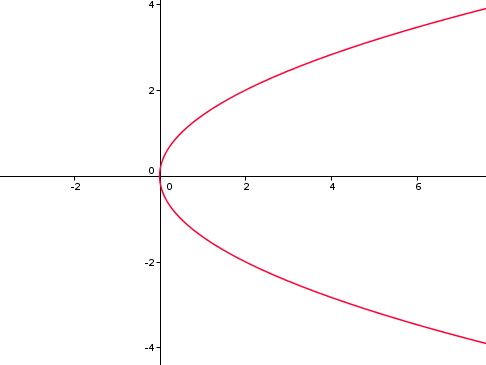
\includegraphics[scale=0.35]{img/parabola2.png}
	\end{center}

	Fibra sobre $\{a\}\in\{\A_k^1 \}$ puede ser varias cosas: $\varphi^{-1}(\{a\})$ puede ser 2 puntos, 1 punto o el vacío
\end{example}

Nuestro objetivo es usar el ideal de definición de W ($\I(W) \subset \K[y_1,...,y_m]$) para calcular la fibra de $\varphi$ sobre $W$.

\obs Como $W \subset Y$, entonces $\I(Y) \subset \I(W)$ por lo tanto $\I(W)$ esta en correspondencia biyectiva con el ideal $\quot{\I(W)}{\I(Y)}$ de $\K[Y]=\quot{\K[y_1,...,y_m]}{\I(Y)}$.

\subsection{Descripción algebraica de la fibra de $\varphi$ sobre $W \subset Y$:}

\begin{align*}
	\varphi: X & \rightarrow Y \\
	(a_1,...,a_n) &  \rightarrow (f_1(a_1,...,a_n),...,f_m(a_1,...,a_n))
\end{align*}

$f_i$ regulares en X.
Y. Por otro lado tenemos el homomorfismo inducido siguiente:

\begin{align*}
\varphi^*: \K[Y] & \rightarrow \K[X] \\
\cls{y_i} & \rightarrow f_i\\
\cls{G(y_1,...,y_n)} & \rightarrow \cls{G(f_1,...,f_m)}
\end{align*}

Sea $(a_1,...,a_n) \in X$ ¿Cuando $\varphi(a_1,...,a_n) \in W$?:

$\varphi(a_1,...,a_n) \in W \Leftrightarrow (f_1(a_1,...,a_n),...,f_m(a_1,...,a_n)) \in W \Leftrightarrow \forall F(y_1,...,y_m) \in \I(W)$ se tiene que $F((f_1(a_1,...,a_n),...,f_m(a_1,...,a_n))=0 \Leftrightarrow \forall F \in \I(W), \psi(F)(a_1,...,a_n)=0$.

\textbf{Conclusión:}

$$ \varphi^{-1}(W)=\left\{ (a_1,...,a_n) \in X \subset \Akn: \forall F \in \I(W), \psi(F)(a_1,...,a_n)=0 \right\} $$

En este diagrama:


\begin{tikzcd}
	\K[Y]=\quot{\K[y_1,...,y_m]}{\I(Y)} \arrow[rightarrow]{rr}{\varphi^*}
	\arrow[leftarrow]{dr}{\pi}
	& & \K[X]=\quot{\K[x_1,...,x_n]}{\I(X)}
	\arrow[leftarrow]{dl}{\psi}\\
	& \K[y_1,...,y_m]&
\end{tikzcd}

En realidad lo que hago es coger $\I(W) \in \K[y_1,..,y_m]$ o $\quot{\I(W)}{\I(Y)} \in \K[Y]$ que es lo mismo. Y los llevo a $\psi(\I(W)) \in \K[X]$.

De aquí deducimos que $\varphi^{-1}(W)=\V(\psi(\I(W))) \subset \Akn$

\begin{example}
	\begin{align*}
	\varphi: \A^2_K & \rightarrow \A^1_K \\
	(a,b) & \rightarrow a
	\end{align*}

	Con $|K|=\infty$

	Fijamos $W=\{a\} \subset \A_K^1$ y queremos calcular $\psi^{-1}(W)$.

	Miramos el homomorfismo de anillos que induce:

	\begin{align*}
	\varphi^*: \K[y_1] & \rightarrow \K[x_1,x_2] \\
	y_1 & \rightarrow x_1
	\end{align*}

	Vemos que $\varphi^*$ es inyectivo. Por tanto por lo que hemos visto otros días $\varphi$ debería ser dominante, y de hecho lo es, ya que es sobreyectivo. Ahora vamos a lo nuevo, a calcular la fibra sobre $\{a\}$.

	Para ello calculo $\I(W)$, y tenemos claramente que $\I(\{a\})=\gen{y_1 -a}$.

	Además $\varphi^*(\gen{y_1-a})=\gen{x_1-a}^e$. (Recordemos lo de elevar a e, que no es más que el extendido. Esto sale de que de normal en un homomorfismo la imagen $J$ de un ideal $I$ no tiene por que ser un ideal, al poner $J^e$ nos referimos al ideal más pequeño que contiene a J)


	Entonces $\varphi^{-1}(W)= \V(\gen{x_1-a}) \subseteq \A^2_K$. Que es una recta como vimos anteriormente.
\end{example}


\begin{example}
	\begin{align*}
	\varphi: P=\{ x_1-x_2^2=0 \} & \rightarrow \A^1_K \\
	(a,b) & \rightarrow a
	\end{align*}

	Con $|K|=\infty$

	\begin{align*}
	\varphi^*: \K[y_1] & \rightarrow \quot{\K[x_1,X_2]}{\gen{x_1-x_2^2}} \\
	y_1 & \rightarrow \cls{x_1}
	\end{align*}

	Sea $W=\{a\} \subset \A^K_1$, entonces $\I(W) = \gen{y_1-a}$, calculo $(\varphi^*(\I(W)))^e=\gen{x_1-a} \subset \quot{\K[x_1,x_2]}{\gen{x_1-x_2^2}}$. Pero ahora CUIDADO, ese ideal no es lo mismo que $\gen{x_1-a} \subset \K[x_1,x_2]$, este último es una recta como en el ejemplo anterior.

	Pero los ideales de $\quot{\K[x_1,x_2]}{\gen{x_1-x_2^2}}$ están en correspondencia biyectiva con los ideales de $\K[x_1,x_w]$ que contengan a $\gen{x_1-x_2^2}$.

	De modo que $\gen{x_1-a} \in \quot{\K[x_1,x_2]}{\gen{x_1-x_2^2}} $ y $ \gen{x_1-a,x_1-x_2^2} \in \K[x_1,x_2]$ están en correspondencia biyectiva y es el que tengo que tomar. Ahora resuelvo el sistema para ver cuál es la v.a.a.: (consideramos $\K=\real$)

	$$
	\left\{ \begin{array}{c}
	x_1=a \\
	x_1-x_2^2=0\\
	\end{array} \right.
	\implies
	\left\{ \begin{array}{c}
	\text{Si } a=0 \implies x_1=0, x_2=0 \\
	\text{Si } a >0 \implies x_1=a, x_2=\pm \sqrt{a}\\
	\text{Si } a < 0 \implies x_1=a, x_2^2<0 \implies \emptyset.\\
	\end{array} \right.
	$$


\end{example}

\obs: En la proyección del primer ejemplo la extension $\K[y_1]$ sobre $\K[x_1,x_2]$ no es finita porque $x_2$ no es entero sobre $\K[y_1]$

Pero en el segundo ejemplo si, ya que hemos añadido $\cls{x_2}$ que es entero  sobre $\K[y_1]$ y por tanto la extensión es finita.


% -*- root: ../AlgebraConmutativa.tex -*-

\chapter{La dimensión de las variedades algebraicas afines}

Esquema de contenidos del tema:

\begin{itemize}
	\item Definición intuitiva de lo que debería ser la dimensión de una v.a.a.
	\begin{itemize}
		\item Traducción de la noción anterior en términos de lo que vamos a llamar dimensión de Krull de un anillo.
		\item Nos vamos a creer que $\dim_{Krull}\K[x_1,...,x_n]=n$ (dimensión de Krull de un anillo de polinomios con coeficientes en un cuerpo).
	\end{itemize}
	\item Veremos que si tenemos $A \subset B$, una extensión entera de anillos, entonces $ \dim_{Krull} A = \dim_{Krull} B$
	\item Vamos a ver el \textbf{Lema de Normalización de Noether:} Toda v.a.a. X se puede proyectar de manera finita sobre un espacio afín $\Akn$, donde $n=\dim_{Krull}\K[X]$. (siendo $\K[X]$ un anillo de coordenadas) %(Enunciado geométrico)
	\item Y si nos diese tiempo veríamos el teorema que nos dice que $\dim_{Krull}\K[x_1,...,x_n]=n$.
\end{itemize}

\section{Definición intuitiva de lo que debería ser la dimensión de una v.a.a.}

Por ejemplo, si tenemos un espacio vectorial V sobre un cuerpo $\K$, para saber la dimensión de V buscamos una base $B=\{ v_1,...,v_n\}$ que es una serie de vectores linealmente independientes que generan el espacio. 

Cada vez que me dan una base puedo construir una cadena de subespacios vectoriales:
$\{0\} \subsetneqq \gen{v_1} \subsetneqq \gen{v_1,v_2} \subsetneqq ... \subsetneqq \gen{v_1,...,v_n}$. Entonces esta cadena es la más larga dentro de $V$, y la longitud de esta cadena se dice que es n (el primero se considera 0). Por tanto $n= \dim V$

Vamos a usar el mismo razonamiento para calcular la dimensión de $X$ v.a.a.. Vamos a suponer $X$ es irreducible y a considerar dentro de $X$ subvariedades y construir la cadena más larga dentro de $X$. Consideramos dentro de $X$ cadenas estrictamente crecientes de subvariedades irreducibles. Tendríamos:

$$Y_0 \subsetneqq Y_1 \subsetneqq ... \subsetneqq Y_n=X$$

Entonces podríamos definir $\dim X$ como la longitud de la cadena más larga.

Si $X$ no fuese irreducible se separa en variedades irreducibles y se le asigna como dimensión el máximo de las longitudes.

\subsection{Traducción de la noción de dimension en términos del álgebra conmutativa} 

Tenemos $X \subseteq  \Akn$, y tenemos también $\I(X) \subseteq \K[x_1,...,x_n]$

La cadena anterior de ideales irreducibles se traduce en una cadena de ideales  primos (por la proposición \ref{prop:VaaIrreducibleIdPrimo}):

$$\I(Y_0) \supsetneqq \I(Y_1) \supsetneqq ... \supsetneqq \I(Y_n)=\I(X)$$

Pero estas cadenas (que contienen a $\I(X)$) se corresponden biyectivamente con cadenas de ideales primos en $\K[X]=\quot{\K[x_1,...,x_n]}{\I(X)}$ . Así, para definir la dimensión de $X$ miraremos al máximo de las longitudes de las cadenas  de ideales primos en $\K[X]$.

Esto es bastante fuerte ya que vimos que dada una v.a.a. $X$ el anillo de coordenadas es el mismo sea donde sea que viva $X$ (dando igual que la $X$ viva en un espacio afín o en otro). Imaginaos que $X$ es una curva en $A^3$, la misma curva la puedo ver en $A^4$, su anillo de coordenadas es el mismo. \textcolor{red}{Donde hemos visto esto?}

\textcolor{red}{Poner reflexion de anillos de coordenadas unicos para variedades dando igual donde viven}

\begin{defn}
	Sea $A$ un anillo y sea $p_0 \subsetneqq p_1 \subsetneqq ... \subsetneqq p_r$ una cadena estrictamente creciente de ideales primos en $A$. En tal caso, diremos que la longitud de la cadena es $r$, y definimos $\dim_{Krull} A$ como el máximo (si existe) de las longitudes tras considerar todas las posibles cadenas de ideales primos en $A$:
	
	$$ \dim_{Krull}A = \max \left\{ r: \exists \text{ cadena } p_0 \subsetneqq p_1 \subsetneqq ... \subsetneqq p_r \text{ con } p_i \text{ primo } \subset A \right\} $$
\end{defn}

\begin{example}
	Sea $\K$ un cuerpo (su único ideal primo es el $\{0\}$), la cadena más larga que puedo montar es $\{0\}$, por tanto: $\dim_{Krull} \K = 0$
\end{example}

\begin{example}
	Sea $\ent$, los ideales primos en $\ent$ son el $\{0\}$ y los generados por números primos, por tanto las cadenas serán:
	
	$$ \{0\} \subsetneqq \gen{p} $$
	
	Pero $\gen{p}$ es maximal así que ya no puedo hacer la cadena más larga, luego $\dim_{Krull} \ent = 1$
\end{example}

\begin{example}
	Sea $\K[x]$ con $\K$ cuerpo. Construyo la cadena:
	
	$$\{0\} \subsetneqq  \gen{p(x)} $$
	
	Con $p(x)$ irreducible, pero $\gen{p(x)}$ es maximal así que ya no puedo seguir. Luego  $\dim_{Krull} \K[x] = 1$
	
	Además $\K[x]$ es el anillo de coordenadas de $\A^1_K$, que esperamos que tenga dimensión 1.
\end{example}

\begin{example}
	Sea $\K[x,y]$:
	
	$$\{0\} \subsetneqq  \gen{x} \subsetneqq \gen{x,y} $$
	
	Por tanto  $\dim_{Krull} \K[x,y] \geq 2$
\end{example}

	Nos vamos a creer lo siguiente: \textbf{Teorema: Sea $\K$ un cuerpo, entonces $\dim_{Krull} \K[x_1,...,x_n]=n$}
	
	\begin{defn}[Dimension de una v.a.a.]
		Sea $X$ una v.a.a. definimos $\dim X = \dk \K[X]$
	\end{defn}
	
\section{Dimensión de Krull en el caso de extensiones enteras de anillos}

Recordatorio extensiones enteras:

Tenemos $A \hookrightarrow B$ ($A \subset B$) extensión de anillos. Cada elemento de b es raíz de un polinomio mónico de elementos en A.
\begin{itemize}
	\item Si $A \subset B$ es una extensión entera y si $J \subset B$ es un ideal, entonces $\quot{A}{J \cap A} \hookrightarrow \quot{B}{J}$ es entera.
	\item Si $S \subset A$ es una parte multiplicativa (conjunto multiplicativamente cerrado) entonces $S^{-1}A \hookrightarrow S^{-1}B$ es una extensión entera.
	\item Si fijamos un ideal primo $p \subset A$ y tomamos $S=A \setminus p$, entonces $A_p=S^{-1}A$ es un anillo local con maximal $pA_p$
	\item \textbf{Teorema:} Sea $A \subset B$ una extensión entera de dominios de integridad. Entonces $A$ es un cuerpo  $\Leftrightarrow B$ es un cuerpo.
\end{itemize}

\begin{prop}
	Sea $A \subset B$ una extensión entera y sea $q \subset B$ un ideal primo (si tengo un homomorfismo de A a B, $f^{-1}(ideal)=ideal$) entonces $q \cap A$ es maximal $\Leftrightarrow$ q es maximal.
	
\end{prop}

\begin{proof}
	Sea $A \subset B$ entera $\implies \underbrace{\quot{A}{q \cap A}}{\text{D.I}} \subset \underbrace{\quot{B}{q}}{\text{D.I}}$ entera.
	
	Por el teorema anterior $\quot{A}{q \cap A}$ es un cuerpo $\Leftrightarrow$ $\quot{B}{q}$ es un cuerpo. Por lo tanto q es maximal si y solo si $q \cap A$ es maximal.
\end{proof}


Vamos a ver ejemplos para ver que la hipótesis sobre la extensión es necesaria:
\begin{example}
	$\ent \subset \rac$ es algebraica pero no entera. En $\rac$ cogemos el único primo que hay que es el $\{0\}$ que además es maximal. Ahora miramos $\ent \cap \{0\}=\{0\}$ que es un primo no maximal.
\end{example}

\begin{example}
	$\ent \subset \ent[x]$ y cogemos $p=\gen{3}=3 \ent[x] \in \ent[x]$. Este ideal es primo ya que al pasar al cociente me sale $\quot{\ent[x]}{\gen{3}}=F_3[x]$ un dominio de integridad, pero no un cuerpo. Por tanto tengo un primo no maximal.
	
	Ahora hago $\ent \cap 3 \ent[x]=3 \ent$ que es un primo maximal.
\end{example}

\begin{prop}
	Sea $A \subset B$ una extensión entera, y sea $p \subset A$ un ideal primo. Entonces existe un ideal primo $q \subset B$ tal que $q \cap A=p$.
\end{prop}

\begin{proof}
	$A \subset B$. Sea un primo $p \subset A$. Buscamos un primo $q \subset B$.
	
	Definimos la siguiente parte multiplicativa. Sea $S=A \setminus p$ una parte multiplicativa en A y en B.
	
	\begin{tikzcd}
		A \arrow[hookrightarrow]{r}{entera}
		\arrow[rightarrow]{d}{\varphi}
		\arrow[rightarrow]{dr}{f (h)}
		&  B
		\arrow[rightarrow]{d}{g}\\
		S^{-1}A=Ap \arrow[hookrightarrow]{r}{entera} & S^{-1}B
	\end{tikzcd}
	
	$Ap$ es un anillo local. ideal maximal $pA_p$.
	
	De modo que:
	\begin{enumerate}
	 	\item $S^{-1}B$ tiene algún ideal maximal $m \subset S^{-1}B$
	 	\item $m \cap A_p$ es un ideal maximal luego necesariamente $m \cap A_p=pA_p$.
		\item $\varphi^{-1}(pA_p)=p$
		\item $f^{-1}(m)=p$ (usando 2 y 3).
		\item $g^{-1}(m)=q$ es un ideal primo en $B$.
		\item $q \cap A = p$ porque el diagrama es conmutativo. $h^{-1}(m)=f^{-1}(m)$.
	\end{enumerate}
\end{proof}

Vamos a ver ejemplos sobre la necesidad de la hipótesis de que la extensión sea entera.
\begin{example}
	$\ent \subset \rac $. Cojo $\gen{3} \in \ent$ primo, no existe ningún ideal primo $q \subset \rac$ tal que $q \cap \ent = \gen{3}$.
\end{example}

\begin{example}
	Sea $\real[x] \subset \quot{\real[x,y]}{\gen{xy-1}}$. El ideal $\gen{x}$ es un ideal primo en $\real[x,y]$, y no existe ningún ideal primo $q \subset  \quot{\real[x,y]}{\gen{xy-1}}$ tal que $q \cap \real[x]=\gen{x}$.
	
	Para ello nos basta probar que $\nexists$ ningún ideal primo en $ \quot{\real[x,y]}{\gen{xy-1}}$ que contenga a $\gen{\cls{x}}^e$ (extendido de x).
	
	$$ \gen{\cls{x}}^e=\gen{1}$$
	
	\begin{align*}
		H=\{xy-1=0\} & \rightarrow \A^1_K \\
		(a,b) & \rightarrow (a)
	\end{align*}
	
	La fibra sobre $\{0\}$ es vacía.
	
	Luego $\real[x] \subset \quot{\real[x,y]}{\gen{xy-1}}$ no puede ser una extensión entera.
\end{example}

\begin{prop}
	Sea $A \subset B$ una extensión entera. Sea $p \subset A$ un ideal primo. Sean $q_1 \subseteq q_2 \subset B$ dos ideales primos tales que $q_1 \cap A=q_2 \cap A = p$. Entonces $q_1=q_2$.
\end{prop}

\begin{proof}
	Sea $S = A \setminus p$
	
	\begin{tikzcd}
		A \arrow[hookrightarrow]{r}{entera}
		\arrow[rightarrow]{d}{\varphi}
		\arrow[rightarrow]{dr}{f (h)}
		&  B
		\arrow[rightarrow]{d}{g}\\
		S^{-1}A=Ap \arrow[hookrightarrow]{r}{entera} & S^{-1}B
	\end{tikzcd}
	
	\begin{enumerate}
		\item 	Como $S= A \setminus p$ entonces $q_1 \cap S = q_2 \cap S = \emptyset$
		\item Por 1, $q_1S^{-1}B$ es primo y $q_2S^{-1}B$ es primo y $q_1S^{-1}B  \subseteq q_2S^{-1}B$. Ambos pertenece a $S^{-1}B$.
		
		\begin{tikzcd}
			A \arrow[hookrightarrow]{r}{entera}
			\arrow[rightarrow]{d}{\varphi}
			\arrow[rightarrow]{dr}{f (h)}
			&  B
			\arrow[rightarrow]{d}{g}\\
			\underbrace{S^{-1}A=Ap}{pA_p} \arrow[hookrightarrow]{r}{entera} & \underbrace{S^{-1}B}{q_1S^{-1}B  \subseteq q_2S^{-1}B}
		\end{tikzcd}
		\item $q_1S^{-1}B \cap A_p=pA_p=q_2S^{-1}B \cap A_p$
		\item $pA_p$ es maximal $\implies q_1S^{-1}B$ y $q_2S^{-1}B$ son maximales, luego $q_1S^{-1}B = q_2S^{-1}B$.
		
		Tenemos que $q_1=g^{-1}(q_1S^{-1}B)$ y $q_2=g^{-1}(q_2S^{-1}B) \implies q_1 = q_2$ 
	\end{enumerate}
	
	Ejemplo para ver la necesidad de las hipótesis:
	
	\begin{example}
		$\ent \subset \ent[x]$. Cojo $\gen{3} \in \ent$ y $\gen{3} \subsetneqq \gen{3,x} \in \ent[x]$ maximal. 
	\end{example}
	
	\begin{example}
		\begin{align*}
			\real[x] & \hookrightarrow \real[x,y] \\
			\gen{x} & \gen{x} \subseteq \gen{x,y}
		\end{align*}
		
		\begin{align*}
			\A^2 & \rightarrow \A^1 \\
			(a,b)& \rightarrow a
		\end{align*}
		
	\end{example}
	
\end{proof}

\begin{corol}
	Sea $A \subset B$ entera. Entonces $\dk A \geq \dk B$
\end{corol}

\begin{proof}
	Sea $q_0 \subsetneqq q_1 \subsetneqq ... \subsetneqq q_r \subset B$ una cadena de ideales prmos en B. Entonces $q_0\cap A \subsetneqq q_1\cap A \subsetneqq ... \subsetneqq q_r\cap A \subset A$
\end{proof}	

%Clase 25/04/2016

\begin{theorem}[Going-up]
	Sea $q_0 \subsetneqq q_1 \subsetneqq ... \subsetneqq q_q \subsetneqq q_{s+1} \subsetneqq ... \subsetneqq q_n$ una cadena de primos en A, y sea $p_0 \subsetneqq p_2 \subsetneqq ... \subsetneqq p_s$ una cadena de primos en B con $p_i \cap A=q_i $ para $i=0,...,s$. Entonces existen primos $p_{s+1} \subsetneqq ... \subsetneqq p_n$ en $B$ tal que $p_s \subsetneqq p_{s+1}$ y $pj \cap A = q_i$ para $j=s+1,...,n$.
\end{theorem}

\begin{proof}
	Podemos suponer que entonces estamos en el caso siguiente:
	\begin{itemize}
		\item $q_0 \subsetneqq q_1$ primos en A.
		\item $p_0$ primo en B. Y se que $p_0 \cap A=q_0$
	\end{itemize}
	
	¿Cómo encontramos $p_1 \subset B$ primo tal que $p_1 \cap A=q_1$ y tal que $p_1 \supsetneqq p_0$?
	
	\begin{tikzcd}
		A \arrow[hookrightarrow]{}{entera}
		\arrow[rightarrow]{d}{\pi}
		\arrow[rightarrow]{dr}{f}
		&  B
		\arrow[rightarrow]{d}{g}\\
		\quot{A}{p_0 \cap B} \arrow[hookrightarrow]{r}{entera} & \quot{B}{p_0}
	\end{tikzcd}
	
	$P_0 \cap B = q_0$. Primo $\cls{q_1}=\quot{q_1}{q_0}$.
	
	Observamos que:
	\begin{enumerate}
		\item $\cls{q_1}=\quot{q_1}{q_0}$ es primo en $\quot{A}{q_0}$
		\item Como $\quot{A}{q_0} \hookrightarrow \quot{A}{p_0}$ es entera, entocnes existe $\cls{p_1} \subset \quot{B}{p_0}$ tal que $\cls{p_1} \cap \quot{A}{q_0}=\cls{q_1}$. 
		\item $f^{-1}(\cls{p_1})=q_1$
		\item $\cls{p_1}$ esta en correspondencia biyectiva con un único primo $p_1 \subset B$ que contiene a $p_0$. $\pi{-1}(\cls{p_1})=p_1$, $p_1 \supseteqq p_0$.
		\item $p_1 \cap A=q_1$ porque el diagrama conmuta.
	\end{enumerate}
\end{proof}

\obs 		
$A \hookrightarrow B$ extensión entera y sea $J \subsetneqq B$ un ideal. Afirmación:

\begin{proof}
$$\quot{A}{J \cap A} \hookrightarrow \quot{B}{J}$$

Es una extension entera porque:

Es inyectiva:

$$ A \hookrightarrow B \rightarrow \quot{B}{J}$$ y la composición g es un homomorfismo. Ahora tenemos:

$$\quot{A}{\ker g} \hookrightarrow \quot{B}{J}$$

Luego $\ker A=A \cap J$. Ahora vamos a ver que:

$$ \quot{A}{J \cap A} \hookrightarrow \quot{B}{J}$$ es una extensión entera.

Sea $\cls{b} \in \quot{B}{J}$, existe $q(x) \in \quot{A}{J \cap A}[x]$ mónico tal que $q(\cls{b})=0$.

\begin{tikzcd}
	A \arrow[hookrightarrow]{}{entera}
	\arrow[rightarrow]{d}{\pi}
	\arrow[rightarrow]{dr}{f}
	&  B
	\arrow[rightarrow]{d}{g}\\
	\quot{A}{J \cap A} \arrow[hookrightarrow]{r}{entera} & \quot{B}{J }
\end{tikzcd}

Sea $b \in B$ un elemnto tal que $b \equiv \cls{b} mod J$. Como b es entero sobre A entonces existe $p(x) \in A[x]$ mónico tal que $p(b)=0$.

$p(x) = a_0+a_1x+...+a_{n-1}x^{n-1}+x^n$ con $a_1 \in A$. Luego $p(b) = a_0+a_1b+...+a_{n-1}b^{n-1}+b^n=0$ en B. Entonces: $a_0+a_1b+...+a_{n-1}b^{n-1}+b^n=\cls{0}$ en $\quot{B}{J}$ y por tanto $\cls{a_0}+\cls{a_1}\cls{b}+...+\cls{a_{n-1}}\cls{b^{n-1}}+\cls{b}^n=\cls{0}$  en $\quot{B}{J}$. $\cls{a_i} \in \quot{A}{J \cap A}$ basta tomar $q(x)=\cls{a_0}+\cls{a_1}x+...+\cls{a_{n-1}}x^{n-1}+x^n=\cls{0}$
\end{proof}

\begin{corol}
	Si $A \subset B$ es entera entonces $\dk B \geq \dk A$
\end{corol}

\textbf{conclusion} Si $A \subset B$ es entera entonces:
$$ \dk A = \dk B $$

\begin{example}
	Sea $\real \subset \quot{\real[x]}{\gen{x(x^2-1)}}$ entonces es como añadirle $\cls{x}$.
	
	$\cls{x}$ es entero sbre $\real$ porque es raíz de $p(T)=T^3-T \in \real[T]$ Como $\cls{x}$ es entero sobre $\real$ entonces $\real \hookrightarrow \quot{\real[x]}{\gen{x^3-x}}$ es finita, por tanto es entera.
	
	\textcolor{red}{incluir duda del tio del primera fila}
	
	$$ \dk \quot{\real[x]}{\gen{x^3-x}} = 0$$
	
	Toda cadena de primos en $\quot{\real[x]}{\gen{x^3-x}}$ tiene longitud 0. Luego en $\quot{\real[x]}{\gen{x^3-x}}$ todos los primos son maximales y minimales. ¿Cuántos puede haber?. Sólo puede haber un número finito de primos porque es un anillo noetheriano (cociente de noetheriano es noetheriano, y en su día dijimos que en un anillo noetheriano sólo hay un número finito de primos minimales)
	
	Cuáles son los primos de $\quot{\real[x]}{\gen{x^3-x}}$, pues estan en correspondencia biyectiva con los de $\real[x]$ que contienen a $\gen{x^3-x}$,, osea que sólo son $\gen{\cls{x}}$, $\gen{\cls{x-1}}$, $\gen{\cls{x+1}}$.
\end{example}

 
\subsection{Interpretación geométrica}

\begin{defn}
	Sean $X,Y$ v.a.a. y sea $\varphi: X \rightarrow Y$ un morfismo. Diremos que $\varphi$ es un morfismo finito si $\varphi^*: \K[Y] \hookrightarrow \K[X]$ es una extensión finita (y por tanto entera).
\end{defn}

\begin{example}
	Sea $|\K|=\infty$, y sea;
	\begin{align*}
		\varphi: P=\{x_2 2-x_1=0 \}& \rightarrow \A^1 \\
		(a,b) & \rightarrow a
	\end{align*}
	 
	 entonces es finita.
	 
	 Porque:
	 \begin{align*}
	 	\varphi^*: \K[y_1]& \rightarrow \quot{K[x_1,x_2]}{\gen{x_2^2-x_1}} \\
	 	y_1 & \rightarrow \cls{x_1}
	 \end{align*}
\end{example}

\subsection{Morfismos finitos}

$\varphi: X \rightarrow Y$ es finito si $\varphi^*: \K[Y] \hookrightarrow \K[X]$ es finito. Es particular $\K[Y] \subset \K[X]$ es una extensión entera.

\begin{theorem}
	Sea $\varphi: X \rightarrow Y$ un morfismo finito. Entonces:
	\begin{enumerate}
		\item $\varphi$ es un morfismo sobreyectivo.
		\item Para cada punto $y \in Y$, el número de preimágenes $#\{ \varphi^{-1}(y) \}$ es un número finito de puntos.
	\end{enumerate}
\end{theorem}

\begin{proof}
	Suponemos que $\K$ es algebraicamente cerrado (para simplifcar la demostración, pero vamos que no es una condición necesaria).
	
	1) Sea $(b_1,...,b_m) \in Y$, queremos probar que existe un punto $(a_1,...,a_n) \in X$ tal que $\varphi(a_1,...,a_n)=(b_1,...,b_m)$. Vamos a calcular la fibra de $\varphi$ sobre $(b_1,...,b_m)$. Para ello consideramos el ideal de definición del punto $(b_1,...,b_m)$ que es $\gen{y_1-b_1,....,y_m-b_m}$
	
	Miramos a:
	
	\begin{align*}
		\varphi^*: \K[Y]  \quot{\K[y_1,...,y_m]}{\I(Y)}& \rightarrow K[X] = \quot{\K[x_1,...,x_n]}{\I(X)} \\
		\gen{y_1-b_1,....,y_m-b_m} & \rightarrow \varphi^*(\gen{y_1-b_1,....,y_m-b_m})^e=J
	\end{align*}
	
	Lo que probamos es que $\varphi^{-1}(b_1,...,b_m)= \V(\varphi^*(\gen{y_1-b_1,....,y_m-b_m})^e)$ queremos ver que es no vacío.
	
	Como $\K[Y] \hookrightarrow \K[X]$ es entera, entonces $\quot{\K[Y]}{\underbrace{J \cap \K[Y]}_{(\varphi^*)^{-1}(J)}}$.
	
	Por tanto ambas tienen la misma $\dk$
	
	En tesumen tenemos:
	\begin{align*}
		\varphi^*: \K[Y]  \quot{\K[y_1,...,y_m]}{\I(Y)}& \rightarrow K[X] = \quot{\K[x_1,...,x_n]}{\I(X)} \\
		\gen{\cls{y_1-b_1},....,\cls{_m-b_m}} & \rightarrow \varphi^*(\gen{y_1-b_1,....,y_m-b_m})^e=J
	\end{align*}
	
	Entonces $\gen{\cls{y_1-b_1},....,\cls{_m-b_m}} \subset (\varphi^*)^{-1}(J)$, pero es más afirmamos que son iguales.
	
	Supongamos que no, entonces $(\varphi^*)^{-1}(J)=\gen{\cls{1}}$.
	
	Ahora:
	
	\begin{enumerate}
		\item Como $\K[Y] \hookrightarrow \K[X]$ es entera, existe un primo $p \subset \K[X]$ tal que $\varphi^{-1}(p)=	\gen{\cls{y_1-b_1},....,\cls{_m-b_m}}$
		
		Pero si yo tengo:
		\begin{align*}
			\varphi^*: \K[Y] =  \quot{\K[y_1,...,y_m]}{\I(Y)}& \rightarrow K[X] = \quot{\K[x_1,...,x_n]}{\I(X)} \\
			\gen{\cls{y_1-b_1},....,\cls{_m-b_m}} & \rightarrow p
		\end{align*}
		
		Entonces $\underbrace{\varphi^*(\gen{y_1-b_1,....,y_m-b_m})^e}_{J} \subset p$. 
		
		Entonces tendríamos que $(\varphi^*)^{-1}(J) \subset (\varphi^*)^{-1}(p)=\gen{\cls{y_1-b_1},....,\cls{_m-b_m}}$. Entonces $(\varphi^*)^{-1}(J) \neq \gen{1}$ y es más: $(\varphi^*)^{-1}(J) = \gen{\cls{y_1-b_1},....,\cls{_m-b_m}}$.
		
		Esto significa que $J \neq \gen{1} \underbrace{\implies}_{\K = \cls{\K}} \V(J) \neq \emptyset \implies \varphi^{-1}((b_1,...,b_m)) \neq \emptyset \implies \varphi$ es sobreyectiva.
		
		\item Veamos que $\varphi^{-1}((b_1,...,b_m))$ consta de un número finito de puntos.
		
		\begin{align*}
			\varphi^*: \K[Y]  \quot{\K[y_1,...,y_m]}{\I(Y)}& \rightarrow K[X] = \quot{\K[x_1,...,x_n]}{\I(X)} \\
			\gen{\cls{y_1-b_1},....,\cls{_m-b_m}} & \rightarrow p
		\end{align*}
		
		\begin{tikzcd}
			\K[Y] \arrow[hookrightarrow]{}{entera}
			\arrow[rightarrow]{d}{\varphi^*}
			&  \K[X]
			\arrow[rightarrow]{d}{g}\\
			\quot{\K[Y]}{J \cap \K[Y]} \arrow[hookrightarrow]{r}{entera} & \quot{\K[X]}{J }
		\end{tikzcd}
		
		De aquí concluimos que $\dk \quot{\K[X]}{J}=0 \implies$ todos los ideales de $\quot{\K[X]}{J}$ son minimales y maximales, y como $\quot{\K[X]}{J}$ es noetheriano $\implies \quot{\K[X]}{J}$ solo tiene un número finito de primos (y son todos maximales) de la punta:
		
		$$ \gen{x_1-a_{11},...,x_n-a_{1n}},...,\gen{x_1-a_{s1},...,x_n-a_{sn}} $$
		
		Entonces $\varphi^{-1}((b_1,...,b_m))= \V(J)=\{ (a_{11},...,a_{1n}),...,(a_{s1},...,a_{sn}) \}$
	\end{enumerate}
\end{proof}

\begin{example}
	
	$|K| = \infty$
	\begin{align*}
		\varphi^*: \K[x,y]& \rightarrow \quot{K[x,y,z]}{\gen{z^4+xyz+3}} \\
		x & \rightarrow \cls{x} \\
		y & \rightarrow \cls{y} \\
	\end{align*}
	Entonces $\cls{z}$ es raíz de $T^4+xyT+3 \in \K[x,y][T]$
	
	\begin{align*}
		\varphi: X=\{ z^4+xyz+3=0  \} & \rightarrow \A^2 \\
		(a,b,c) & \rightarrow (a,b)
	\end{align*}
	
	Suponemos $\K= \cls{\K}$ ($\K$ algebraicamente cerrado).
	
	Caculamos la fibra sobre (0,0):
	
	\begin{align*}
		\gen{x,y} & \rightarrow \varphi^*(\gen{x,y})^e \\
	\end{align*}
	
	$z^4+xyz+3=0$ con $x=0$ e $y=0$, entonces $z^4+3=0$ hay 4 maximales:
	
	$$\gen{x,y,z- \sqrt[4]{3}} \Leftrightarrow (0,0,\sqrt[4]{3})$$
	$$\gen{x,y,z- \sqrt[4]{3}e^{\frac{2 \pi i}{4}} \Leftrightarrow (0,0,\sqrt[4]{3}e^{\frac{2 \pi i}{4}}$$
	$$\gen{x,y,z- \sqrt[4]{3}e^{\frac{4 \pi i}{4}}$$
		$$\gen{x,y,z- \sqrt[4]{3}e^{\frac{6 \pi i}{4}}$$	
			
			
	Podríamos haber calculado la fibra sobre (2,1):
	\begin{align*}
		\gen{x-2,y-1} & \rightarrow \varphi^*(\gen{x-2,y-1})^e \\
	\end{align*}
	
	Y tendríamos que resolver $z^4+xyz+3=0$ con $x=2$ e $y=1$. Y resolveríamos $z^4+2z+3=0$ y tendríamos la siguiente solución:
	$$\varphi^{-1}((2,1))=\{ (2,1,\alpha_1), (2,1,\alpha_2),(2,1,\alpha_3), (2,1,\alpha_4) \}$$
\end{example}

\begin{example}
	Consideramos $|K| = \infty$
	
	\begin{align*}
		\varphi^*: \K[x]& \rightarrow \quot{K[x,y]}{\gen{xy}} \\
		x & \rightarrow \cls{x}
	\end{align*}
	
	\begin{align*}
		\varphi: X=\{ xy=0  \} & \rightarrow \A^1_K \\
		(a,b) & \rightarrow a
	\end{align*}
	
	Vemos que la fibra sobre el $0$ es toda una recta  y sobre cualquier otro punto es sólo un punto.
	
	Fibra sobre (0):
	\begin{align*}
		\gen{x} & \rightarrow \varphi^*(\gen{x})^e \\
	\end{align*}
	
	Y tengo que resolver el sistema $xy=0$ y $x=0$.
\end{example}

%% Apéndices (ejercicios, exámenes)

\appendix

% -*- root: ../AlgebraConmutativa.tex -*-

\chapter{Resumen rápido}

\section{Anillos I: ideales, homomorfismos y cocientes}

\subsection{Anillos}

Partimos del anillo (\fref{def:Anillo}), un conjunto con operaciones suma y producto (ambas conmutativas), asociativo y distributivo con respecto al producto y al que nosotros pediremos además que tenga una unidad multiplicativa. Podemos poner adjetivos a los elementos de anillos según su comportamiento:

\begin{itemize}[itemsep = -2pt]
\item \textbf{Unidad}: Elemento con inverso multiplicativo.
\item \textbf{Divisor de cero}: Elemento que multiplicado por otro da cero.
\item \textbf{Nilpotente}: Elemento que elevando a una cierta potencia da cero.
\end{itemize}

Igualmente, podemos poner clasificar los anillos según sus comportamientos:

\begin{itemize}[itemsep = -2pt]
\item \textbf{Dominio de integridad}: sin divisores de cero.
\item \textbf{Anillo reducido}: sin nilpotentes distintos de cero
\item \textbf{Cuerpo}: Todo elemento no nulo tiene inverso multiplicativo.
\item \textbf{Anillo local}: Sólo con un ideal maximal.
\item \textbf{Anillo semilocal}: Con un número finito de maximales.
\end{itemize}

\subsection{Ideales}

Como siempre, nos interesará estudiar los subanillos (anillo contenido dentro de otro) y especialmente los ideales (\fref{def:Ideal}). Un subconjunto $I ⊆ R$ será ideal si no es vacío, es subgrupo con la suma y tiene la propiedad de absorción ($r∈I,\,i ∈ I \implies ri ∈ I$). A la hora de las demostraciones, no hará falta demostrar que es subgrupo con la suma, nos valdrá demostrar que $a,b ∈ S \implies a+b ∈S$ ó $a-b ∈ S$ (\fref{prop:def_ideal2} y  \ref{prop:def_ideal3}). Sobre los ideales podemos sacar varias operaciones:

\begin{itemize}[itemsep = -2pt]
\item \textbf{Generación}: Dado $T ⊂ R$, construimos el ideal que lo contiene como $\gen{T} = \set{\sum r_i t_i\tq r_i ∈ R\,t_i ∈ T}$.
\item \textbf{Intersección}: La intersección de ideales es ideal.
\item \textbf{Unión/suma de ideales}: La unión en general no es ideal, así que definimos la suma (\fref{def:IdealSuma}) como $I+J = \set{a+b \tq a ∈ I, \, b∈J}$ que sí es un ideal.
\item \textbf{Producto}: De forma análoga a la suma (\fref{def:IdealProducto}).
\item \textbf{Radical de un ideal}: Elementos del anillo que tienen alguna potencia en el ideal. En particular, el nilradical será el ideal de los nilpotentes. Además, $\sqrt{I} = \bigcap \pideal$ donde $\pideal$ son ideales primos de $R$ que contienen a $I$.
\end{itemize}

Al igual que con los anillos, podemos poner adjetivos a los ideales:

\begin{itemize}[itemsep = -2pt]
\item \textbf{Propio}: Distinto del todal.
\item \textbf{Radical}: Si su radical es él mismo.
\item \textbf{Primo}: $I \subsetneq R$ tal que $a · b ∈ I \implies a∈I$ ó $b ∈I$.
\item \textbf{Maximal}: Ideal propio maximal con respecto a la inclusión de ideales (\fref{def:IdealMaximal}).
\item \textbf{Principal}: Generado por un único elemento.
\item \textbf{Primo minimal}: Primo y minimal con respecto a la inclusión de primos.
\end{itemize}

Un teorema importante (\ref{thm:IdealContenidoMaximal}) es ver que cualquier ideal propio está contenido en un maximal de $R$. Para la demostración se usa el \nref{lem:Zorn}, que nos dice que un conjunto no vacío parcialmente ordenado con cualquier cadena creciente acotada tiene un maximal.

En general, los ideales maximales nos dan cosas interesantes: cualquier maximal es primo, y además si en un anillo todos los ideales son primos es un cuerpo.

\subsection{Homomorfismos}

Un homomorfismo de anillos (\fref{def:Homomorfismo}) es una aplicación $f$ compatible con la suma y el producto, y que además nos lleva la unidad multiplicativa en unidad multiplicativa. Una propiedad muy útil es que $f$ es inyectiva si y sólo si $\ker f = \zerogen$. La imagen de ideales por $f$ no tiene por qué ser ideal, pero la inversa de ideales sí que es ideal.

\subsection{Cocientes}

Dado un ideal $I$, se define una relación de equivalencia $a \sim b \iff a - b ∈ I$ que nos permite definir el conjunto cociente $\quot{R}{I}$ como el conjunto de clases de equivalencia de $R$ módulo $I$. El conjunto cociente es igualmente anillo conmutativo con unidad, y la aplicación paso al cociente π que lleva cada elemento a su clase es un homomorfismo. π es sobreyectiva y $\ker π = I$.

Además de las propiedades de homomorfismos, π nos lleva ideales de $R$ en ideales de $\quot{R}{I}$, y $\inv{π}(π(L)) = L + I$. También respeta la inclusión de ideales que contienen a $I$ (si $I ⊆ M \subsetneq L$ entonces $π(M) \subsetneq π(L)$) y la primalidad (ideales primos en $R$ son primos en el cociente).

El anillo cociente nos permite estudiar ideales. $I$ es primo sii $\quot{R}{I}$ es dominio de integridad; es maximal sii $\quot{R}{I}$ es cuerpo y es radical sii $\quot{R}{I}$ es reducido.

\subsection{Teoremas de isomorfía}

Los teoremas de isomorfía nos dan, atención, isomorfías. Dado un homomorfismo $\appl{f}{R}{S}$, el \nref{thm:IsomorfiaAnillos1} nos dice que hay un isomorfismo $\quot{R}{\ker f} \simeq \img f$ y un homomorfismo inducido $\appl{\bar{f}}{\quot{R}{\ker f}}{S}$.

Más generalmente (\fref{prop:FactorizacionHomomorfismo} y \ref{prop:FactorizacionHomomorfismo2}) $I ⊂ \ker f$ si y sólo si $f$ factoriza por el homomorfismo $\appl{f'}{\quot{R}{I}}{S}$ (en otras palabras, si y sólo si $f = f' ○ π$ donde π es el paso al cociente).

El \nref{thm:IsomorfiaAnillos2} nos dide que dados $I ⊂ J ⊂ R$ ideales de un anillo, entonces $\quot{R}{J} \simeq \frac{\quot{R}{I}}{\quot{J}{I}}$ o, en otras palabras, que el $I$ se puede ``cancelar'' y es lo mismo. Este teorema nos da una demostración sencilla para ver que la imagen inversa de un ideal primo es otro primo.

Por último, el \nref{thm:IsomorfiaAnillos3} nos dice que dados $I,J$ ideales en $R$ entonces $\quot{I+J}{I} \simeq \quot{J}{I ∩ J}$.

\section{Anillos II: Módulos y más}

\subsection{Módulos}

Dado $R$ un anillo, un $R$-módulo es un grupo abeliano con la suma con una operación externa $R×M \to M$ que cumple unas propiedades sensatas, a saber, distributividad por la izquierda y derecha, asociatividad ($r(r'm) = (rr')m$) y unidad ($\one_R · m = m$).

Un $R$-módulo estará finitamente generado si cualquier elemento es combinación lineal finita de elementos de $r$ por una ``base'' de elementos de $M$.

\subsection{Localización multiplicativa}

Una parte multiplicativa es un conjunto cerrado con el producto, que nos permite construir el localizado de $R$, dado por $\inv{S}R = \quot{R×S}{\sim}$ donde $(r,s) \sim (r',s') \iff ∃s'' ∈ S \tq s''(rs'-r's) = 0$. Una primera propiedad es ver que $\inv{S}R = \set{0}$ si y sólo $S$ contiene nilpotentes.

\seprule[Fin temario parcial 1]

Dos propiedades rápidas sobre la localización: tomando el homomorfismo de inclusión $ψ(r) = (r,1)$ de $R$ en $\inv{S}R$, tenemos las siguientes propiedades (ver \fref{thm:PropsLocalizacion}):

\begin{itemize}
\item $ψ(s)$ es invertible para $s ∈ S$.
\item $ψ(a) = 0$ si y sólo si $as = 0$ para algún $s ∈ S$.
\item Cualquier elemento de $\inv{S}R$ se puede expresar como $ψ(r) · \inv{f}(s)$.
\end{itemize}

Además, esas propiedades determinan completamente a $\inv{S}R$: si tenemos otro homomorfismo $\appl{f}{R}{B}$ que cumple esas propiedades entonces $B \simeq \inv{S}R$.

\begin{wrapfigure}[9]{R}{0.4\textwidth}
\vspace{-15pt}
\centering
\begin{tikzpicture}
\matrix (m) [matrix of math nodes,row sep=4em,column sep=2em,minimum width=2em]
{
	R &  &  B\\
	& S^{-1}R &  \\};
\path[-stealth]
(m-1-1) edge node [above] {$f$} (m-1-3)
(m-1-1) edge node [below] {$\psi$} (m-2-2)
(m-2-2) edge node [right] {$g$} (m-1-3);
\end{tikzpicture}

\caption{Diagrama conmutativo para la propiedad universal de la localización.}
\label{fig:Resumen:PropUnivLocalizacion}
\end{wrapfigure}


Sin embargo, el teorema verdaderamente relevante de esta parte es la \nlref{thm:PropUniversalLoc}, que nos dice que existe una única aplicación $g$ que hace conmutar el diagrama de la \fref{fig:Resumen:PropUnivLocalizacion}.

\subsection{Ideales y localización}

La localización funciona decentemente con los ideales, y se cumplen varias propiedades interesantes:

\begin{itemize}
\item Dado un ideal $J ⊂ \inv{S}R$, entonces $\psi(\psi^{-1}(J))^e = J$.
\item Dado un ideal $I ⊂ R$, entonces $\psi^{-1}(\psi(I)^e)=\bigcup_{s\in S}(I:s)$ con $(I:s)=\set{ r \in R \tq r\cdot S \in I }$.
\item Dado un ideal $I ⊂ R$, entonces $\psi^{-1}(\psi(I)^e)=R \iff I \cap S \neq \emptyset$.
\item Todo ideal de $\inv{S} R$ es el extendido de algún ideal de $R$.
\end{itemize}

Para ideales primos, se cumplen las siguientes tres propiedades:

\begin{itemize}
\item Si $\pideal \cap S \neq \emptyset \implies \psi(\pideal)^e=S^{-1}R$.
\item Si $\pideal \cap S = \emptyset \implies \psi(\pideal)^e$ es un ideal primo en $S^{-1}R$.
\item Hay una correspondencia biyectiva entre ideales primos $\pideal ⊂ R$ que no intersecan con $S$ ($\pideal ∩ S = ∅$) y los ideales primos de $\inv{S} R$.
\end{itemize}

Para terminar, dos formas de construir localizados. Dado un $a ∈ R$, construimos la parte multiplicativa $S = \set{a^n}_{n ∈ ℕ}$ y entonces definiremos $R_a ≝ R_{\set{a}} ≝ \inv{S} R$ como $R$ localizado en $a$.

Por otra parte, si tomamos $\pideal ⊂ R$ un ideal primo en $R$, entonces definimos $S = R \setminus \pideal$ y $R_\pideal ≝ \inv{S}R$ como $R$ localizado en el ideal primo \pideal. En particular, $R_\pideal$ es un \nlref{def:AnilloLocal}.

\subsection{Anillos noetherianos}

Un \nlref{def:AnilloNoetheriano} es un anillo para el cual todo ideal es finitamente generado como $R$-módulo. Los dominios de ideales principales (donde todos los ideales están generados por un único elemento) o los cuerpos son dos ejemplos de anillos noetherianos.

Hay dos caracterizaciones útiles para anillos noetherianos (\fref{prop:caracterizacion_noetheriano}). Que $R$ sea noetheriano es equivalente a

\begin{itemize}
\item Toda cadena creciente de ideales estabiliza: $I_1 ⊆ I_2 ⊆ \dotsb I_n = I_{n+1} = I_{n+2} = \dotsb$.
\item Todo conjunto no vacío de ideales en $R$ tiene un elemento maximal (no tiene por qué ser un ideal maximal).
\end{itemize}

Además, el \nref{thm:tma_base_hilbert} nos dice que si $R$ es noetheriano, entonces $R[x]$ es noetheriano.

Por último, los pasos al cociente y al localizado conservan ``noetherianidad'': si $R$ es noetheriano y $I ⊂ R$ un ideal, entonces $\quot{R}{I}$ es noetheriano igualmente (\fref{prop:NoetherianoCociente}), y si $S ⊂ R$ es una parte multiplicativa entonces $\inv{S}R$ también es noetheriano (\fref{prop:NoetherianoLocalizacion}).

% -*- root: ../AlgebraConmutativa.tex -*-
\chapter{Ejercicios}

Últimamente nos llegan comentarios de gente que dice que "los apuntes están muy bien, pero me daba vergüenza deciros que el ejercicio $X.Y$ estaba mal". Gracias.

Pero si tú te beneficias de estos ejercicios y crees que están mal, por favor háznoslo saber por email o en persona.

El profesor no va a tener ningún reparo en ponernos un 0 en el examen.

\setcounter{section}{-1} % Start counting from 0
\section{Hoja 0}

\begin{problem}
Sea $R$ un anillo. Demuestra que:

\ppart Si $a \in R$ es un divisor de cero, entonces $a$ no puede ser una unidad.
\ppart Si $R$ es finito, entonces todo $r \in R \setminus \set{0}$ es o bien unidad, o bien un divisor de cero
\ppart Si $R$ no es finito, el enunciado anterior no es necesariamente cierto.
\solution

\doneby{Guille}

\spart

Si $a$ es un divisor de cero, entonces $∃b ∈ R$, con $b ≠ 0$ tal que $ab = 0$. Si $a$ fuese una unidad, podríamos multiplicar por su inverso a ambos lados, y tendríamos que $a'ab = a' 0 \implies b = 0$, contradicción.

\spart

Dado un $r ∈ R^*$, consideramos todas las posibles multiplicaciones por $b ∈ R^*$. Si existe algún $b ∈ R^*$ tal que $rb = 1$, entonces $r$ es una unidad. Si, por otra parte, $rb = 0$, entonces $r$ es divisor de cero.

Vamos a demostrar ahora que el último caso ($r$ no es unidad ni divisor de cero) no se puede dar. Dado que $R$ es finito, por el principio del palomar tiene que haber dos multiplicaciones por elementos distintos que repitan resultado, esto es, $∃b,c ∈ R^*$ tales que $rb = rc$ y $b ≠ c$. Sin embargo, simplemente operando tenemos que $rb - rc = 0$, y por la propiedad asociativa $r(b-c) = 0$, por lo que $r$ sí es divisor de cero, contradicción.

\spart

El principio del palomar no nos vale en cuerpos infinitos. Por ejemplo, en $ℤ$ sólo hay dos unidades y no hay divisores de cero.
\end{problem}

\begin{problem}
Encuentra todas las unidades y los divisores de cero en $\ent$, $\ent_n$ y en $\K[x]$ donde $\K$ es un cuerpo. % de ahí las dos patitas que diría Quirós
\solution
\end{problem}

\begin{problem}
{\bf Sobre las unidades en anillos de polinomios}

Sea $R$ un anillo y sea $R[x]$ el anillo de polinomios con coeficientes en $R$.
\ppart Si $R$ es un dominio de integridad demuestra que
\[ \set{\text{Unidades de } R[x]} = \set{\text{Unidades de } R} \]
\ppart Demuestra, dando un contraejemplo, que el enunciado anterior no es cierto si $R$ no es un dominio de integridad.
\solution

\doneby{Guille}

\spart

Un dominio de integridad no tiene divisores de cero, por lo que nunca nos vamos a poder quitar los monomios de $x^n$ y sólo nos van a quedar las unidades de $R$.

Más formalmente, sea $p(x) = a_0 + a_1 x + \dotsb + a_nx^n$ y $q(x) = b_0 + b_1 x + \dotsb + b_mx^m$ unidades, tales que $p(x) q(x) = 1$. Sin embargo, $p(x) q(x)$ va a tener como coeficiente más alto $a_n b_n x^{m+n}$, y si $p$ y $q$ son unidades el coeficiente de $x^{m+n}$ ha de ser cero para $m+n ≥ 1$. Por lo tanto, o bien $m = n = 0$ y ambos polinomios son de grado cero (luego unidades de $R$) o bien $a_n b_n = 0$, que ya hemos dicho que no ocurre por ser $R$ dominio de integridad.

\spart

Tomamos $ℤ_4[x]$ y $p(x) = 2x + 1$, $q(x) = -2x + 1$. Multiplicando, $p(x) · q(x) = -4x^2 +2x -2x + 1 = 1 \mod 4$, por lo que son unidades de $R[x]$ a pesar de no ser polinomios de grado 0.

\end{problem}

\begin{problem}
Demuestra, dando un contraejemplo, que el conjunto de todos los divisores de cero de un anillo, junto con el 0 no forman, en general, un ideal.
\solution

\doneby{Guille}

Tomamos $ℤ_{6}$, que tiene como divisores de cero $\set{2,3,4}$. Sin embargo, no es un grupo con la suma ya que $2 + 3 = 5$, que no es un divisor de cero.


\end{problem}

\begin{problem}
Demuestra, dando un contraejemplo, que el conjunto de todos los elementos de un anillo que no son unidades no forman, en general, un ideal.
\solution
\end{problem}

\begin{problem}
Demuestra que las siguientes afirmaciones son equivalentes:
\ppart $R$ es un dominio de integridad
\ppart el ideal $\zerogen$ es primo en $R$
\ppart el ideal $\zerogen$ es primo minimal en $R$
\solution
\end{problem}

\begin{problem}
Demuestra que las siguientes afirmaciones son equivalentes:
\ppart $R$ es un cuerpo
\ppart $R$ solo tiene dos ideales, $\zerogen$ y $R$
\ppart El único maximal de $R$ es $\zerogen$
\solution
\end{problem}

\begin{problem}
Sea $\K$ un cuerpo finito
\ppart Demuestra que $\K$ es una extensión finita de $\field_p$ con $p = \mop{char} (\K)$. Concluye que $|\K| = p^n$ para algún $n \geq 1$, $n \in \nat$.
\ppart Demuestra que el homomorfismo de Frobenius que eleva cada elemento a la potencia p es un isomorfismo. Concluye que $\K$ es un cuerpo perfecto.
\ppart Demuestra que $\K$ es un cuerpo de descomposición para el polinomio $x^{p^n}-x$.

Sugerencia: observa que $\K^*$ es un grupo multiplicativo con $p^n - 1$ elementos, concluye que todos los elementos de $\K$ son raíces de $x^{p^n}-x$.
\ppart Deduce del apartado anterior que todos los cuerpos con $p^n$ elementos son isomorfos y que para cada natural $n \geq 1$ hay un cuerpo con $p^n$ elementos. Denotamos por $\field_{p^n}$ al único cuerpo salvo isomorfismo con $p^n$ elementos.
\ppart Usa el apartado c) para demostrar que si $n|m$ entonces $\field_{p^n} \subset \field_{p^m}$ y la extensión es de grado $m/n$.
\ppart Si $\field_{p^n} \subset \field_{p^m}$ demuestra que la extensión es simple.

Sugerencia: usa el Teorema del elemento primitivo.
\ppart Concluye que $\K$ es finito, entonces para cada natural $m \geq 1$, existe al menos un polinomio irreducible de grado m.

Sugerencia: usa los dos apartados anteriores.
\solution

\doneby{Guille}

Dado que no sé si esto lo hemos visto en la teoría, definimos la característica de un cuerpo y la extensión finita.

\begin{defn}[Característica\IS de un cuerpo]
Dado un cuerpo $(\K, +, ·)$, definimos su característica como el número de veces que tenemos que sumar la identidad multiplicativa consigo misma para tener la identidad de la suma. Esto es, si un cuerpo tiene $\mop{char} \K = p$, entonces $\underbracket{\one + \one + \dotsb + \one}_{p\text{ sumas}} = \zero$.
\end{defn}

\begin{defn}[Extensión\IS de cuerpos] \citep[Def. I.1]{apuntesGalois}
Dados dos cuerpos $F$ y $E$ tales que $F⊆E$ diremos que $E$ es una extensión de $F$.

Se escribe $F⊆E$ (obviamente) o también $E/F$.
\end{defn}


\begin{defn}[Grado\IS de una extensión] \citep[Def I.3]{apuntesGalois}
Sea $E/F$ una extensión de cuerpos.
El grado de la extensión es la dimensión de $E$ como espacio vectorial sobre $F$, es decir, \[[E:F] = \dim_FE \]
\end{defn}

Diremos que una extensión es una \concept{Extensión\IS finita} cuando su grado es finito.

\spart

Tenemos que demostrar que \K tiene un subanillo isomorfo a $ℤ_p$ (el hecho de que la extensión finita viene gratis por ser \K finito). Si la característica de \K es $p$, eso significa que $\underbracket{\one + \one + \dotsb + \one}_{p\text{ sumas}}= \zero$. Podemos considerar entonces $\gen{\one} = ℤ_p$, que es un cuerpo (trivial) y además es un subcuerpo de \K, ya que lo hemos generado con las sumas de $n$ veces la unidad, que por definición están en \K.

Falta ahora demostrar que $\card\K = p^n$ para algún $n ≥ 1$. Esto lo sacamos de \citep[Ej. 1.4]{apuntesGalois}. Definimos un homorfismo de anillos $φ$ de la siguiente forma: \begin{align*} \appl{φ}{ℤ&}{K} \\
α &\longmapsto α · \one
\end{align*}

Estudiemos el núcleo de φ. Son los elementos de $ℤ$ cuya imagen es la unidad en $\K$, esto es, tomando $n = \mop{char}(\K)$, \[ \ker φ = \set{a·n \tq a ∈ ℤ} = nℤ \]

El segundo teorema de isomorfía de grupos\footnote{Ver magníficos apuntes de Pedro Valero de Estructuras Algebraicas \citep{apuntesEA}.} nos dice que existe un isomorfismo entre la imagen de $φ$ y el grupo cociente $\quot{ℤ}{\ker φ}$, al que llamaremos $γ$:

\[ \appl{γ}{\quot{ℤ}{nℤ}}{\img φ ⊆ \K} \]

Afirmamos que $n≠0$: $\K$ es finito y $\quot{ℤ}{0ℤ} = ℤ$, así que no puede existir un isomorfismo entre ambos.

Afirmamos que $n$ es primo, y vamos a demostrarlo por reducción al absurdo. Supongamos $n = ab$. Si operamos en $\fd_n$, tenemos que $n\equiv 0 \mod n$ y entonces $ab=0$. Aplicamos $γ$ a ambos lados y tendríamos que $γ(a)·γ(b) = γ(0) = 0_\K$, contradicción ($\K$ es un cuerpo así que no puede tener divisores de $0$).

Sea $p=n$, entonces \[ \mathbb{F}_p = \quot{ℤ}{nℤ}  \simeq \img φ \] es un subcuerpo de $\K$, luego $\K$ es un espacio vectorial sobre $\mathbb{F}_p$. Es decir, que si $[\K:\mathbb{F}_p] = m$, entonces $\{x₁, \dotsc, x_m\}$ es base de $\K$ sobre $\mathbb{F}_p$, luego \[ \card{\K} = \card{\fd_p}^{[\K:\fd_p]} = p^m\] para $m ≥ 1$, y ya tenemos lo que buscábamos.

Una observación importante: el cuerpo finito de $n$ elementos \textbf{no es} $\quot{ℤ}{nℤ}$. Los enteros módulo $n$ sólo son un cuerpo cuando $n$ es primo. Es decir, que en general \[ \fd_n ≠ \quot{ℤ}{nℤ} \].

Los cuerpos finitos hay que construirlos específicamente como el cociente de un cuerpo finito de orden primo con el ideal generado por un polinomio irreducible. Por ejemplo, podríamos preguntarnos si hay un cuerpo con 9 elementos. Existe, porque $9=3^2$.

\spart

A modo de nota, por ser $\K$ un cuerpo es un dominio de integridad (no tiene divisores de cero) y por lo tanto si tiene característica $p$, $p$ debe ser primo\footnote{Si tuviésemos que $p$ no es primo, lo podemos descomponer como producto factores primos $p = a_1·a_2\dotsb a_n$ con $a_i ≠ \one$. Entonces $\zero = p · \one = a_1\one · a_2 \one \dotsb a_n \one = \zero$, pero como no tenemos divisores de cero alguno de esos $a_i \one$ debe ser cero, y por lo tanto el cuerpo tiene característica $a_i$, con $a_i$ primo.}.


Denotaremos el \concept{Homomorfismo\IS de Frobenius} como $φ(x) = x^p$. Probamos primero que es compatible con las operaciones. Vemos que \[ φ(a+b) = (a+b)^p = \sum_{n=0}^p \comb{p}{n} a^{p-n} b^n \], sin embargo, salvo para $n = 0$ y $n = p$, los coeficientes serán divisibles por $p$ y por lo tanto serán $0$. Entonces $φ(a+b) = a^p + b^p = φ(a) + φ(b)$, luego φ es compatible con la suma. La compatibilidad con el producto es trivial.

Vamos a comprobar ahora que es biyectivo. Tenemos $a, b ∈ \K$ distintos, y supongamos que $φ(a) = φ(b)$. Entonces, $0 = φ(a) - φ(b) = φ(a-b) = (a-b)^p$. Ahora bien, por ser \K un cuerpo (y sin divisores de cero por lo tanto) sólo puede ser $a-b = 0$, por lo que $a$ y $b$ son iguales, contradicción.

Por último, para que sea sobreyectivo tenemos que ver que para todo $a ∈ \K$ existe un $b ∈ \K$ tal que $φ(b) = a$. La cuestión es que como \K es un cuerpo finito y ya hemos demostrado que φ es inyectivo no queda otra opción: por el principio del palomar, si nos quitamos un elemento de la imagen de $φ$, habría un $c ∈ \K$ que es imagen de dos elementos de \K y entonces φ no sería inyectivo.

La definición de \concept{Cuerpo\IS perfecto} es esta misma: que el homomorfismo de Frobenius es un automorfismo (isomorfismo consigo mismo).

\spart

Por el Teorema de Lagrange, el orden de cualquier elemento de un grupo tiene que dividir al orden del grupo. Dado que $\K^*$ es un grupo con la multiplicación de orden $p^n - 1$, por lo que $∀x ∈ \K^*$ tenemos que $x^{p^n - 1} = \one$. Si operamos, tenemos que \[  x^{p^n - 1} = \one \implies x^{p^n} = x \implies x^{p^n} - x = 0 \]

Por lo tanto, todos los elementos en $\K^*$ son ceros de ese polinomio. Trivialmente vemos que \zero también es cero de ese polinomio, por lo tanto todos los elementos de \K son raíces.

\spart

\K es el cuerpo de descomposición del polinomio $x^{p^n} - x$, y los cuerpos de descomposición existen y son únicos salvo isomorfismo\footnote{Vía Wikipedia, yo me lo creo.}.

\spart

Si $n|m$, podemos decir que $m = kn$ para algún $k ∈ ℕ$. Los elementos de ambos cuerpos $\field_{p^n}$ y $\field_{p^m}$ son raíces de los polinomios $x^{p^n} -x$ y $x^{p^m} - x$ respectivamente. Ahora bien, $p^m = p^{kn} = (p^n)^k$, y por lo tanto $x^{p^m} = x^{(p^n)^k} = x^{p^n · p^n \dotsb p^n} = (((x^{p^n})^{p^n})^{p^n})^{\dotsb} = x$, por lo que todo $x ∈ \field_{p^n}$ es raíz de $\field_{p^m}$ y por lo tanto $x ∈ \field_{p^m}$.

\spart

Primero definimos qué es una extensión simple.

\begin{defn}[Extensión\IS simple] Una extensión de cuerpos $L/K$ es una extensión simple de grado $n$ si existe un elemento primitivo $X ∈ L$ tal que \[ L = K(X) = \set{a + a_1 X + \dotsb + a_{n-1}X^{n-1}\tq a_i ∈ K} \]

Por ejemplo, $ℚ(\sqrt{2})$ son los números de la forma $a + b\sqrt{2}$ y es una extensión simple de $ℚ$.
\end{defn}

\begin{theorem}[Teorema\IS del elemento primitivo] Sea $L/K$ una extensión finita y separable. Entonces, es una extensión simple.
\end{theorem}

Con esto ya tenemos el ejercicio hecho: el apartado anterior nos dice que $\field_{p^n} ⊂ \field_{p^m}$ es una extensión y por ser finita es simple gracias al teorema del elemento primitivo.

\spart

Si $\K = \field_{p^n}$ es finito, entonces siempre podemos encontrar un cuerpo $\field_{p^{nm}}$ cuya extensión sea de grado $\frac{nm}{n} = m$, que por el teorema del elemento primitivo está generada por un elemento $X ∈ \field_{p^{nm}}$. Por ser una extensión de grado $m$, tenemos que $X^m ∈ \field_{p^n}$ (si no, sería una extensión de grado superior). En ese caso, $x^{mn} - X^{m}$ es un polinomio que tiene como raíz $X$ y por lo tanto se nos va a quedar algún factor de grado mayor que uno irreducible en $\field_{p^n}$.

\end{problem}

%%%%%%%%%%%%%%%%%%%%%%%%%%%%%%%%%%%%%%%%%%%%%%%%%%%%%%%%%%%%%%%%%%%%%%%
\section{Hoja 1: Anillos, ideales}

\begin{problem}
{\bfseries El radical de un ideal.}

Sea $I\subset R$ un ideal  y sea $\sqrt{I}$ su radical.

\ppart Demuestra que $\sqrt{I}$ es un ideal que además contiene a $I$.

\ppart Demuestra que todo ideal primo es radical.

\ppart Describe todos los ideales de ${\mathbb Z}$ que sean radicales.

\ppart Sea $\K$ un cuerpo. Describe todos los ideales de $\K[x]$ que sean radicales.

{\em Sugerencia: utiliza el ejercicio 1  de la parte de problemas para entregar.}

\solution

\doneby{Guille}

Recordamos la definición de \nlref{def:RadicalIdeal}: son los elementos del anillo que tienen una potencia en el ideal.

\spart

Primero tenemos que comprobar que el radical está cerrado por la suma. Sean $a,b ∈ \sqrt{I}$ tales que $∃m,n ∈ ℕ$ con $a^m ∈ I,\;b^n ∈ I$. Supongamos, sin pérdida de generalidad, que $m > n$. Queremos ver que $a+b ∈ \sqrt{I}$ o, equivalentemente, que $∃s ∈ ℕ$ tal que $(a+b)^s ∈ I$. Podemos tomar $s = m + n$, de tal forma que el desarrollo en serie de potencias sea \[ (a+b)^s = \sum_{k=0}^{m+n} \comb{m+n}{k} a^{m+n-k}b^k \]

Para $k = 0, \dotsc, m$, tendremos que $a^{m+n-k} = a^m·a^{n-k} ∈ I$ por absorción ($a^m ∈ I$). Cuando $k > m$, tendremos que $b^k ∈ I$ por la misma razón, por lo que siempre tendremos que los elementos de la suma estarán en $I$ y entonces $(a+b)^s ∈ I$.

La propiedad de absorción es considerablemente más sencilla: si $a∈\sqrt{I}$ con $a^m ∈ I$, entonces $∀b ∈ R$ tendremos que $(ba)^m = b^m a^m ∈ I$.

\spart

Un ideal es primo (\fref{def:IdealPrimo}) cuando cada vez que $a · b ∈ I$, se tiene que $a ∈ I$ o $b ∈ I$. Dado que ningún elemento de $I$ sale del producto de elementos de fuera de $I$, podemos escribir $I = \gen{a_1, \dotsc, a_n}$, esto es, $I$ está generado por elementos de $I$ multiplicados por sí mismos o por elementos de $R$. De aquí podemos construir otro ideal $S = \gen{a_1^{m_1}, \dotsc, a_n^{m_n}}$, que seguirá siendo un ideal y del cual $I$ es radical. % Triplazo.

\spart

% No me apetece

\spart

Por una parte, tendremos todos los radicales de $\K$, y $\gen{x}$. \textit{No me apetece pensarlo mucho más, probablemente esté mal.}

\end{problem}

\begin{problem}
{\bfseries Unión de ideales.}

La unión de ideales no siempre es un ideal.

\ppart Sean $I,J\subset R$ dos ideales. Demuestra que, en general, $I\cup J$ no es un ideal.

\ppart  Sea $I_1\subset I_2\subset \ldots \subset I_n \subset \ldots$  una sucesión creciente (no necesariamente finita) de ideales en $R$.
Demuestra que la unión $\cup_{n}I_n$ es un ideal en $R$.

\ppart Demuestra que en ${\mathbb Z}$, $\langle n\rangle +\langle m\rangle=\langle k\rangle$ con $k=\text{gcd}(n,m)$.
\solution
\end{problem}

\begin{problem}
{\bfseries Intersección de ideales.}

La intersección de ideales siempre es un ideal que no hay que confundir con el producto de ideales.

\ppart Sea $\{I_i\}_{i\in {\mathcal I}}$ una colección de ideales.  Demuestra que $\cap_{i\in {\mathcal I}} I_i$ es un ideal en $R$.

\ppart  Demuestra que en ${\mathbb Z}$, $\langle n\rangle \cap \langle m\rangle=\langle k\rangle$ con $k=\text{m.c.m.}(n,m)$.

\ppart  Sean $I, J\subset R$ dos ideales. Demuestra que $I\cdot J\subset I\cap J$; encuentra un ejemplo para el que la inclusión sea estricta.
\solution
\end{problem}

\begin{problem}
{\bfseries ¿Cuándo es la intersección de ideales igual al producto?}

Se dice que dos ideales $I, J\subset R$ son coprimos si $I+J=R$.

\ppart Encuentra dos ideales coprimos en
$Z$, y otros dos en ${\mathbb R}[x,y]$.

\ppart Demuestra que si $I$ y $J$ son coprimos, entonces  $I\cdot J=I\cap J$.

\ppart Sean $I_1,\ldots I_n$ ideales en $R$. Demuestra, usando inducción en $n$, que si los ideales son primos dos a dos entonces $\prod_iI_i=\cap_iI_i$.

\noindent{\em Sugerencia para (a): si $I$ y $J$ son coprimos, entonces existen $x\in I$ e $y\in J$ tales que $x+y=1$;
ahora multiplica la expresión anterior por  $a\in I\cap J$.

Sugerencia para (b): define $J=\prod_{I=1}^{n-1}I_i$; como los ideales $I_i$ son coprimos dos a dos, existen $y_i\in I_n$, y
$x_i\in I_i$, $i=1,\ldots, n-1$, tales que $x_i+y_i=1$; ahora utiliza el producto $\prod_{i=1}^{n-1}x_i$ para probar que
$I_n$ y $J$ son coprimos. }
\solution
\end{problem}

\begin{problem} \label{ej:Hoja1:5}
{\bfseries La geometría que veremos.}

Sean $I_1,\ldots, I_n$ ideales en $R$, y sea $\mathfrak p \subset R$ un ideal primo que contiene a
$\cap_iI_i$, esto es, $\cap_iI_i\subset \mathfrak p$. Demuestra que:

\ppart $I_i\subset \mathfrak p$ para algún $i\in \{1,\ldots,n\}$;

\ppart Si además  $\cap_iI_i=\mathfrak p$ entonces $I_i=\mathfrak p$ para algún $i\in \{1,\ldots,n\}$.

\noindent{\em {Sugerencia para (a)}: si $ I_i \nsubseteq \mathfrak p$ para $i=1,\ldots,n$ entonces para cada $i$ existe un elemento $b_i\in I_i $ con $b_i\notin \mathfrak p$; ahora considera $\prod_ib_i$. }

\solution

\doneby{Guille}

\spart

Seguimos la sugerencia y demostramos por reducción al absurdo: no existe ningún $I_i$ tal que $I_i ⊆ \mathfrak{p}$. Por lo tanto, para cada $i = 1, \dotsc, n$ existe un $b_i ∈ I_i$ con $b_i ∉ \mathfrak{p}$. Consideramos ahora $\prod b_i$, que podemos expresar como \[ \prod_{i=1}^n b_i = b_k · \prod_{\substack{i = 1 \\ i ≠ k}}^n b_i \eqreasonup[∈]{Absorción} I_k \]

Como tenemos que el producto está en $I_k$ para todo $k$, tenemos que $\prod b_i ∈ \bigcap I_i$ y entonces $\prod b_i ∈ \mathfrak{p}$. Ahora bien, $\mathfrak{p}$ es primo, por lo que si el producto de todos esos elementos está en $\mathfrak{p}$, entonces su producto ha de estar obligatoriamente en $\mathfrak{p}$, contradicción.

\spart

De nuevo por reducción al absurdo. Si $I_i ≠ \mathfrak{p}$, entonces para cada $i = 1, \dotsc, n$ existe un $b_i ∈ I_i$ y (al menos un) $j = 1, \dotsc, n$, $j ≠ i$, con $b_i ∉ I_j$ de tal forma que $b_i ∉ \mathfrak{p}$.

\end{problem}

\begin{problem}
{\bfseries Miramos ejemplos en $\ent$.}

En ${\mathbb Z}$ observa que $\langle 36\rangle \subset \langle 3\rangle$, $\langle 2\rangle$;
encuentra todas las maneras de escribir $\langle 36\rangle$ como intersección de ideales. A la vista del problema anterior,  ¿qué crees que va a suceder?
\solution
\end{problem}

\begin{problem}
{\bfseries Anillos locales.}

Demuestra que las siguientes afirmaciones son equivalentes:

\ppart $R$ es un anillo local con ideal maximal $\mathfrak m$;

\ppart $R$ contiene un ideal  $\mathfrak m$ tal que todo elemento de $R\setminus \mathfrak m$ es una unidad.
\solution
\end{problem}

\begin{problem}
Sea $k$ un cuerpo. Definimos el anillo de series formales en una variable sobre $k$ como el conjunto
$$k[|t|]:=\left\{\sum_{i=0}^{\infty}a_it^i: a_i\in k\right\}$$
con la suma y el producto habituales. Demuestra que $\alpha=\sum_{i=0}^{\infty}a_it^i
  \in k[|t|] $ es una unidad si y sólo si $a_0\neq 0$. Concluye que $k[|t|]$ es un anillo local cuyo único ideal maximal es además  principal.
\solution
\end{problem}

\noindent \fbox{{\bfseries  Problemas para entregar (CORREGIDOS!)} }

\textbf{Pongo las correcciones de Ana en azul}

% --------------------------------------------------- %
% ----------------- PROBLEMA 1.9 -------------------- %
% --------------------------------------------------- %
\begin{problem}
{\bfseries Sobre los ideales en $K[x]$. Sea K un cuerpo}

\ppart Demuestra que $K[x]$ es un dominio euclídeo.
\ppart Demuestra que en $K[x]$ todos los ideales son principales.
\ppart Demuestra que en $K[x]$ un ideal es maximal si y solo si está generado por un polinomio irreducible.
\ppart Demuestra que en $K[x,y]$ no todos los ideales son principales. {\em Sugerencia: considera el conjunto $I$ formado por todos los polinomios $p(x,y)\in K[x,y]$ que se anulan en $(0,0)$; demuestra que es un ideal y que no es principal.}

\solution


\begin{defn} \textbf{Dominio Euclídeo}
	Es un par $(K, \phi)$ donde $K$ es un dominio de integridad y $\phi$ es una aplicación norma euclídea, es decir: $\phi: K \setminus \{0\} \rightarrow \nat$ cumple:
	\begin{enumerate}
		\item Si $a,b \in K \setminus \{0\}$, se cumple que $a | b \implies \phi(a) \leq \phi(b)$
		\item $\forall a,b \in K$, con $b \neq 0$, $\exists q,r \in K$ tal que $a=bq+r$ con $r=0$ ó $\phi(r) < \phi(b)$
	\end{enumerate}
\end{defn}

Para demostrar que $K[x]$ es un dominio euclídeo, tenemos que definir una aplicación $\phi$ que sea norma euclídea.

Sea $\phi$ una aplicación que asigna a cada polinomio su grado, $\phi(p(x)) = \mop{gr} p(x)$. Vamos a probar que $\phi: K[x] \setminus \{0\} \rightarrow \nat$ es una aplicación norma euclídea:
\begin{enumerate}
	\item Si tenemos $p(x) | q(x)$, entonces quiere decir que $q(x)=p(x)\cdot r(x)$, con $r(x) \in K[x] \setminus \{0\}$. Es obvio que el grado de $p(x)$ es menor o igual que el grado de $p(x)\cdot r(x)$.
	\item Sea $a(x), b(x) \in K[x]$, con $b(x) \neq 0$, tenemos que ver que existe $r(x), q(x) \in K[x]$ tal que $a(x)=b(x)q(x)+r(x)$ con $r(x)=0$ ó $\mop{gr} r(x) < \mop{gr} b(x)$.

	Eso también es cierto. Utilizando el algoritmo de la división (\textcolor{blue}{por inducción en el grado de $b$}), existen $q,r \in K[x]$ tales que $c=bq+r$ con $r=0$ ó $\phi(r) < \phi(b)$.
\end{enumerate}

\spart


\begin{defToUse}
	\begin{itemize}
		\item \textbf{Ideal}: Sea $(R,+,\cdot)$ un anillo y sea $I \subseteq R$. Se dice que $I$ es un ideal si:
		\begin{enumerate}
			\item $I \neq \emptyset$
			\item $(I, +)$ es un subgrupo de R.
			\item Propiedad de absorción: $\forall i \in I, \forall r \in R \implies r\cdot i \in I$.
		\end{enumerate}
		\item \textbf{Ideal generado por $T$}: Definimos el ideal generado por $T$ como el ideal más pequeño de $R$ que contiene a $T$ y se denota por $\gen{T}$.

		Explícitamente, sea $R$ un anillo y $T \subset R$ no vacío, entonces:
		$$ \gen{T} = \{r_1t_1+...+r_st_s: r_i \in R, t_i \in T, s \geq 1 \} $$.
		\item \textbf{Ideal principal}: Un ideal es principal si está generado por un único elemento.
	\end{itemize}
\end{defToUse}

Sea $K[x]$ dominio euclídeo, y sea $I$ un ideal de $K[x]$. Por definición, $I$ es subgrupo normal de $K[x]$. Si $I=\set{0}$ es claro que es un ideal principal. Supongamos entonces que $I$ contiene al menos un elemento distinto de 0.

Sea $a \in I$, tal que $\phi(a) \leq \phi(c)$ para cualquier otro $c\in I$. Entonces, utilizando el algoritmo de la división, existen $q,r \in K$ tales que $c=qa+r$ con $r=0$ ó $\phi(r) < \phi(a)$.

Pero $r=c-qa \in I$, $r \neq 0$, implicaría $\phi(r) \geq \phi(a)$, por la definición de $a$, en contra de las hipótesis del algoritmo de la división. Por tanto, tendríamos que tener $r=0$, y todo elemento $c\in I$ es de la forma $c=qa$, por tanto, $I=\gen{a}$.

\spart


\begin{defToUse}
	\nref{def:IdealMaximal}: Un ideal $I \subsetneq R$ es maximal si cualquier otro ideal que lo contenga es o bien él mismo o bien el total.
\end{defToUse}


En el apartado anterior hemos demostrado que todos los ideales son principales, esto es, están generados por un único elemento. Sea $I$ un ideal generado por $p(x) ∈ K[x]$ irreducible. Para que otro ideal $J = \gen{q(x)}$ contenga a $I$, $q(x)$ tiene que dividir a $p(x)$. Sin embargo, por ser $p(x)$ irreducible, $q(x)$ sólo puede ser o bien $q(x)$ (y entonces $J = I$) o bien $1$ (y entonces $J = K[x]$).

Para la implicación al otro lado, vemos que si $\gen{p(x)} = I \subsetneq K[x]$ es maximal, entonces no hay ningún ideal propio que lo contenga. Por lo tanto, si consideramos cualquier otro ideal $J = \gen{q(x)}$ con $q(x) ≠ 1,\,q(x) ≠ p(x)$, tenemos que $I \subset J$ o, equivalentemente, no existe ningún $q(x)$ que divida a $p(x)$ (salvo $1$ y $p(x)$, que ya hemos excluido). Es decir, $p(x)$ es irreducible.

\spart

Este ejercicio se resuelve cogiendo ejemplos y proposiciones vistos en teoría.

Consideramos el ideal $I=\set{p(x,y)\in K[x,y]\tq p(0,0)=0 }$. Primero vamos a ver que es un ideal:
\begin{enumerate}
	\item $I \neq \emptyset$ porque $0 \in I$
	\item $(I,+)$ es un subgrupo.

	Hay que comprobar que $I$ contiene al 0 (elemento identidad), que es cerrado con $'+'$ y que contiene los elementos inversos, pero como hemos visto esto es equivalente a probar que $\forall p(x,y), q(x,y) \in I$, entonces $p(x,y)-q(x,y) \in I$ (ya que con la suma, el inverso de $q(x,y)$ es $-q(x,y)$).

	Como $p(0,0)=0=q(0,0)$, evidentemente $p(0,0)-q(0,0)=0$ y por tanto $p(x,y)-q(x,y) \in I$.

	\item Si escogemos $r(x,y) \in \rac[x,y]$ y si $p(x,y) \in I$, tenemos que ver que $r(x,y)\cdot p(x,y) \in I$. Obvio ya que $p(0,0)=0 \implies r(0,0)\cdot p(0,0) = 0$
\end{enumerate}

Ahora usamos una proposición vista en teoría, para probar que ese conjunto esta generado por dos elementos, $'x'$ e $'y'$.

Sea $K$ un cuerpo, y sea el ideal $\gen{x,y}$ en $K[x,y]$, entonces:
$$\gen{x,y}=\{p(x,y)\in K[x,y]:p(0,0)=0 \}$$.

Que la tenemos demostrada en los apuntes como sigue:
\begin{itemize}
	\item $\subset)$ Hemos visto que $\gen{x,y}=\{s(x,y) x+r(x,y) y: s(x,y),r(x,y) \in K[x,y] \}$. Es obvio que $s(x,y) x+r(x,y) y$ se anula en el $(0,0)$.
	\item $\supset)$ Sea $p(x,y) \in K[x,y]$ tal que $p(0,0)=0$. Tenemos que $p(x,y)=a_0+a_1x+a_2y+a_3x^2+...+a_nx^ny^m$. Entonces $p(0,0)=a_0=0$. Por tanto, si $a_0=0$, entonces $p(x,y)$ se puede expresar como $r(x,y)y+s(x,y)x$.
\end{itemize}

%Ana dijo que había que añadir algo más, y me dijo esto a grandes rasgos:
%-------------------------------------------------
\textcolor{blue}{
Hemos visto que $x$ e $y$ generan el ideal, pero no hemos probado que ese ese ideal pueda estar generado por otro $p(x,y)$. Es decir, no hemos probado que $\gen{x,y}=\gen{p(x,y)}$.
}

\textcolor{blue}{
Supongamos que sí existe, es decir: $\exists p(x,y) \in K[x,y]$ tal que $\gen{x,y}=\gen{p(x,y)}$.
}

\textcolor{blue}{
Eso quiere decir que $\exists  q(x,y) \in K[x,y]$ tal que $x=q(x,y)\cdot p(x,y)$. Pero $K[x,y]$ es un dominio de factorización única, y $x$ es irreducible, por tanto $x = u\cdot p(x,y)$ con $u$ unidad. Es decir, $p(x,y)=u\cdot x$.
}

\textcolor{blue}{
Por otro lado, también $\exists  s(x,y) \in K[x,y]$ tal que $x=s(x,y)\cdot p(x,y)$. Entonces nos quedaría que $y=s(x,y)\cdot u \cdot x$, pero y es irreducible, y por tanto, esto es imposible.
}
%------------------------------------------------

Por tanto hemos encontrado un ideal que no es principal en $K[x,y]$ porque está generado por dos elementos.
\end{problem}


% --------------------------------------------------- %
% ----------------- PROBLEMA 1.10 -------------------- %
% --------------------------------------------------- %
\begin{problem}
Decide de manera razonada para qué valores de $n$ el anillo ${\mathbb Z}_n$ es un anillo local. En aquellos casos en los que se trate de un anillo local indica cuál es el (único) ideal maximal.

\solution


\begin{defToUse}
	\begin{itemize}
		\item \textbf{Anillo local}: Un anillo es local si sólo tiene un ideal maximal.
	\end{itemize}
\end{defToUse}

El anillo $\ent_n$ es un anillo local para $n=p^m$, para p primo y $m \in \nat$. El único ideal maximal de esos anillos es el ideal $\gen{\cls{p}}$.

Vamos a probarlo:
Sea $\ent_{p^m}$. Vamos a ver que $\gen{\cls{p}}$ es su único ideal maximal. Sabemos que $a\in \gen{\cls{p}}$ si $a=kp$ para algún $k\in \nat$.

Sea $b \in \ent_{p^m}$ tal que $\cls{b} \neq k\cls{p}$, $\forall k \in \nat$. Entonces $b \nmid p \implies b \nmid p^m \implies \mop{mcd} (b,p^m) =1 \implies \gen{b} = \ent_{p^m}$.

Hemos probado que cualquier elemento que no pertenezca a ese ideal, genera todo el conjunto. Por tanto $\gen{\cls{p}}$ es maximal, y para $n=p^m$ tenemos que $\ent_n$ es local.

Falta probar que si $n \neq p^m$, entonces $\ent_n$ no es local. Pero $\ent$ es un dominio de factorización única, por tanto, si $n \neq p^m$, nos queda como única opción que $n=p_1^{m_1}p_2^{m_2}\dotsb p_s^{m_s}$ con $s > 1$, $p_1,\dotsc,p_n$ primos. Y en ese caso, $\gen{p_1}$, $\gen{p_2},\dotsc,\gen{p_s}$ serían ideales maximales distintos los unos de los otros.

\end{problem}


% --------------------------------------------------- %
% ----------------- PROBLEMA 1.11 -------------------- %
% --------------------------------------------------- %
\begin{problem}
Considera el siguiente subanillo de ${\mathbb Q}(x)$:
$$R ≝\left\{\frac{p(x)}{q(x)}: \frac{p(x)}{q(x)} =\frac{r(x)}{s(x)} \text{ con }  s(0)\neq 0\right\}. $$
\ppart  Demuestra que  ${\mathfrak m} ≝ \left\{\frac{p(x)}{q(x)}\in R: p(0)=0\right\}$ es un ideal en $R$.
\ppart  Demuestra que $R$ es un anillo local con ideal maximal $\mathfrak m$.

{\em Sugerencia: puedes usar el ejercicio 7.}

\solution


\spart
\begin{defToUse}
	\begin{itemize}
		\item \textbf{Ideal}: Sea $(R,+,\cdot)$ un anillo y sea $I \subseteq R$. Se dice que $I$ es un ideal si:
		\begin{enumerate}
			\item $I \neq \emptyset$
			\item $(I, +)$ es un subgrupo de R.
			\item Propiedad de absorción: $\forall i \in I, \forall r \in R \implies r\cdot i \in I$.
		\end{enumerate}

		Así como la definición alternativa:

		Sea $(R,+,\cdot)$ un anillo y sea $I \subseteq R$. Se dice que $I$ es un ideal si
		\begin{enumerate}
			\item $I \neq \emptyset$
			\item $\forall a,b \in I$, entonces $a-b \in I$.
			\item Propiedad de absorción
		\end{enumerate}
	\end{itemize}
\end{defToUse}

Para ver si $\mathfrak{m}$ es un ideal vamos a comprobar si cumple las 3 propiedades de los ideales:

\begin{enumerate}
	\item $\mathfrak{m} \neq \emptyset$, es cierto ya que el elemento $\frac{x}{1} \in \mathfrak{m}$.
	\item $(\mathfrak{m},+)$ es un subgrupo. Como hemos visto esto es equivalente a probar que $\forall \frac{p_1(x)}{q_1(x)}, \frac{p_2(x)}{q_2(x)} \in \mathfrak{m}$, entonces $\frac{p_1(x)}{q_1(x)}- \frac{p_2(x)}{q_2(x)} \in \mathfrak{m}$.

	Operando:
	$$\frac{p_1(x)}{q_1(x)}- \frac{p_2(x)}{q_2(x)} = \frac{p_1(x)q_2(x)}{q_1(x)q_2(x)}- \frac{p_2(x)q_1(x)}{q_2(x)q_1(x)}=\frac{p_2(x)q_1(x)-p_1(x)q_2(x)}{q_2(x)q_1(x)}=\frac{t(x)}{q_2(x)q_1(x)}$$

	Como partíamos que $p_1(0)=0=p_2(0)$, entonces $t(0)=0$
	\item Si escogemos $\frac{p_1(x)}{q_1(x)} \in R$ y $\frac{p_2(x)}{q_2(x)} \in \mathfrak{m}$, tenemos que ver que $\frac{p_1(x)}{q_1(x)}\cdot \frac{p_2(x)}{q_2(x)} = \frac{p_1(x)p_2(x)}{q_1(x)q_2(x)} \in \mathfrak{m}$. Obvio ya que $p_2(0)=0 \implies p_1(0)p_2(0) = 0$
\end{enumerate}

\spart
Basándonos en la sugerencia, vamos a probar que todo $ \frac{p(x)}{q(x)} \in R \setminus \mathfrak{m} $ es una unidad.

Así, sea $a=\frac{p(x)}{q(x)}$ tal que $q(0) \neq 0$ y $p(0) \neq 0$. Entonces, el elemento $\frac{q(x)}{p(x)}$ es el inverso multiplicativo de $a$, ya que $\frac{p(x)}{q(x)}\cdot \frac{q(x)}{p(x)}=1$. Por tanto si $a \in R \setminus \mathfrak{k}$ entonces $a$ es unidad. Y por el ejercicio 7 tenemos que $R$ es un anillo local con ideal maximal $\mathfrak m$ si y sólo si $R$ contiene un ideal $\mathfrak m$ tal que todo elemento de $R\setminus \mathfrak m$ es una unidad.

Por tanto, queda demostrado que $R$ es un anillo local con ideal maximal $\mathfrak m$.

\end{problem}


% --------------------------------------------------- %
% ----------------- PROBLEMA 1.12 -------------------- %
% --------------------------------------------------- %
\begin{problem}
{\bfseries Conductores.}
Sean $I, J\subset R$ ideales. Definimos el conductor de $J$ en $I$ \index{Conductor} como:
$$(I:J) ≝\{a\in R: aJ\subset I).$$

\ppart Demuestra que $(I:J)$ es un ideal en $R$ que además contiene a $I$.

\ppart Calcula $(\langle 12\rangle : \langle n \rangle)$ para todo  $n\in {\mathbb Z}$.

\ppart Intuitivamente,  ?`qué es el ideal $(I: \langle a\rangle)$ para $a\in R$?

\ppart Sea ${\mathfrak p}\subset R$ un ideal primo. Calcula $({\mathfrak p}: I)$ para todo $I\subset R$.
?`Por qué crees que obtienes ése   resultado?

\ppart Demuestra que si $J=\langle a_1,\ldots, a_r\rangle$ entonces $(I:J)=\cap_{i=1}^r(I: \langle a_i\rangle).$

\solution

\spart


\begin{defToUse}
	\begin{itemize}
		\item \textbf{Ideal}: Sea $(R,+,\cdot)$ un anillo y sea $I \subseteq R$. Se dice que $I$ es un ideal si:
		\begin{enumerate}
			\item $I \neq \emptyset$
			\item $(I, +)$ es un subgrupo de R.
			\item Propiedad de absorción: $\forall i \in I, \forall r \in R \implies r\cdot i \in I$.
		\end{enumerate}

		Así como la definición alternativa:

		Sea $(R,+,\cdot)$ un anillo y sea $I \subseteq R$. Se dice que $I$ es un ideal si
		\begin{enumerate}
			\item $I \neq \emptyset$
			\item $\forall a,b \in I$, entonces $a-b \in I$.
			\item Propiedad de absorción
		\end{enumerate}
	\end{itemize}
\end{defToUse}

Para ver si $(I:J)$ es un ideal vamos a comprobar si cumple las 3 propiedades de los ideales:

\begin{enumerate}
	\item $(I:J) \neq \emptyset$, es cierto ya que el $\zero \in (I:J)$.
	\item $((I:J),+)$ es un subgrupo. Como hemos visto esto es equivalente a probar que $\forall a, b \in (I:J)$, entonces $a-b \in (I:J)$.

	Cierto ya que si $a \in (I:J)$, entonces \textcolor{blue}{$aJ=\{a\cdot j: j\in J\} \subset I$ (y no $aJ=\{a_1,...,a_j\} \subset I$, ya que no sabemos qe es finito)}, y si $b \in (I:J)$, entonces \textcolor{blue}{$bJ=\{b\cdot j: j\in J\} \subset I$ (y no $bJ=\{b_1,...,b_j\} \subset I$, ya que no sabemos qe es finito)}. Por tanto sean $a_i \in aJ$ y $b_k \in bJ$ entonces $a_i-b_k \in I$ $\forall i,k$ porque $I$ es un ideal y por tanto $(I,+)$ es un subgrupo. Por tanto $(a-b)J \subset I$ y $a-b \in (I:J)$.
	\item Si escogemos $a \in R$ y $b \in (I:J)$, tenemos que ver que $a\cdot b \in (I:J)$. Cierto ya que si $b \in (I:J)$, entonces $bJ=\{b_1,...,b_j\} \subset I$, y como $I$ es un ideal, por la propiedad de absorción $a\cdot b_i \in I$ $\forall i \in [1,j]$. Entonces $a\cdot b\cdot J \subset I$ y  $a \cdot b \in (I:J)$.
\end{enumerate}

\spart
Tenemos que \[ (\gen{12} : \gen{n }) = \{ a \in R: a\gen{n} \subset \gen{12} \} =  \gen{\frac{\mop{mcm}(12, n)}{n}} \]

En otras palabras, $\gen{\frac{\mop{mcm}(12, n)}{n}}$ está formado por elementos $a$ tales que $a·\gen{n} ⊂ \gen{12}$ o, en otras palabras, todos los números que multiplicados por un múltiplo de $n$ sean un múltiplo de $12$. Si $a ∈ \gen{\frac{\mop{mcm}(12,n)}{n}}$, entonces es de la forma $a = k · \frac{\mop{mcm}(12,n)}{n}$ para $k ∈ ℤ$. Este elemento, multiplicado por un elemento de $\gen{n}$, será múltiplo de 12.

\spart

$$(I: \gen{a}) =  \{ b \in R: b \gen{a} \subset I \} $$

Consiste en el ideal que conecta $<a>$ con $I$, ya que coge todos los elementos $b \in R$ tal que $b\cdot \gen{a} \in I$.

De ahí puede venir el nombre de conductor, que se puede interpretar como que $(I:\gen{a})$ son los elementos de $R$ que conducen $\gen{a}$ a $I$.

\spart


\begin{defToUse}
	\begin{itemize}
		\item \textbf{Ideal primo}: Diremos que un ideal $I\subset R$ es primo si $I\neq R$ y si cada vez que $a\cdot b \in I$ se tiene que $a\in I$ o $b\in I$.
	\end{itemize}
\end{defToUse}

Por definición, $(\mathfrak{p}: I) = \set{ a \in R: a I \subset \mathfrak{p} }$. Por ser $\mathfrak{p}$ primo se cumple que si $a·b ∈ \mathfrak{p}$, entonces o bien $a ∈ \mathfrak{p}$ o bien $b ∈ \mathfrak{p}$. Luego hay dos opciones: si $I ⊆ \mathfrak{p}$, entonces $(I:J) = R$ (cualquier elemento del anillo multiplicado por un elemento de $\mathfrak{p}$ será elemento de $\mathfrak{p}$). Si por el contrario $I \nsubseteq \mathfrak{p}$, entonces $(I:J) = \mathfrak{p}$.

\spart

Calculamos el conjunto directamente:
\begin{align*}
	(I:\gen{a_1,\ldots, a_r})
	&= \{ b\in R \tq b \gen{a_1,\ldots, a_r} \subset I \} = \textcolor{blue}{\text{ Hay que probar esta igualdad} }  \\
	&= \{ b\in R \tq b\gen{a_1}, b\gen{a_2},\dotsc ,b\gen{a_r} \subset I \} = \\
	&= \{ b\in R \tq b\gen{a_1} \subset I\} \cap \dotsb \cap \{ b\in R \tq b\gen{a_r} \subset I\} =  \\
	&= \bigcap_{i=1}^r (I: \gen{a_i})
\end{align*}

\textcolor{blue}{
	Demostramos primero que $\{ b \in R: bJ \subset I \} \subset \bigcap (I:\gen{a_i})$.
	\begin{align*}
		& \{ b\in R \tq b \gen{a_1,\ldots, a_r} \subset I \} = \\
		& \{ b\in R \tq b \cdot(a_1s_a+...+a_rs_r) \subset I, \forall s_1,...,s_r \in R \} \implies \\
		&  b\gen{a_1} \subset I \text{ , } \dotsb \text{ , } b\gen{a_r} \subset I =  \\
		&= \bigcap_{i=1}^r (I: \gen{a_i})
	\end{align*}
	}

	\textcolor{blue}{Ahora demostramos que $\bigcap (I:\gen{a_i}) \subset (I:J) $.}

	\textcolor{blue}{Sea $b \in \bigcap (I:\gen{a_i})$, entonces $\forall i=1,\cdots,r$ y $\forall s \in R$. Entonces, $b\cdot s\cdot a_i \in I$. Queremos ver si $b \in (I:\gen{a_1,\ldots, a_r})$.}

	\textcolor{blue}{Sea $l_1a_1+...+l_ra_r \in \gen{a_1,\ldots, a_r}$. Entonces queremos ver si $b(l_1a_1+...+l_ra_r) \in I$. Lo cual es cierto ya que eso es igual a:}

	\textcolor{blue}{$$ \underbrace{bl_1a_1}_{\in I}+\underbrace{bl_2a_2}_{\in I}+...+\underbrace{bl_ra_r}_{\in I} \in I $$}


\end{problem}


\section{Hoja 2: Homomorfismos, cocientes y teoremas de isomorfía}

\begin{problem} Sea $\appl{f}{R}{S}$ un homomorfismo de anillos.

\ppart Demuestra que si $u$ es una unidad en $R$ entonces $f(u)$ es una unidad en $S$.
\ppart Si $a ∈ R$ no es una unidad, ¿puede ser $f(a)$ una unidad en $S$?
\ppart Si $b ∈ R$ es un divisor de cero, ¿es $f(b)$ necesariamente un divisor de cero en $S$?
\ppart Si $b$ no es divisor de cero en $R$, ¿puede ser $f(b)$ un divisor de cero en $S$?

\solution

\doneby{Guille}

\spart

Si $u$ es unidad, entonces $∃\inv{u} ∈ R$, luego $f(u·\inv{u}) = f(1) = 1$, y por otro lado $1 = f(u\inv{u}) = f(u) · f(\inv{u})$, luego efectivamente $f(u)$ es unidad en $S$.

\spart

Sí puede ser. Un contraejemplo sencillo es ver el homomorfismo de anillos de la inclusión $\appl{f}{ℤ}{ℚ}$ dado por $f(a) = a$. Cualquier $n ∈ ℤ \setminus \set{0,1}$ no tiene inverso en $ℤ$ pero sí en $ℚ$.

\spart

No tiene por qué. Si $b$ es divisor de cero, entonces $∃a ∈ R$ tal que $a · b = 0$. Dado que $f(0) = 0$ por ser homomorfismo de anillos, tendremos que $0 = f(a·b) = f(a)·f(b)$ por lo que $f(b)$ será sólo divisor de cero si $f(a)$ y $f(b)$ son distintos de cero.

\spart

Supongamos que $b ∈ R$ no es divisor de cero pero $f(b)$ sí lo es. Eso significa que existe un $c ∈ S$ tal que $s · f(b) = 0$. La cuestión es que los homomorfismo de anillos no tienen por qué ser sobreyectivos, por lo que no es necesario que haya un $a ∈ R$ tal que $f(a) = c$.

\end{problem}

\begin{problem} \textbf{Homomorfismos desde cuerpos}. Demuestra las siguientes afirmaciones

\ppart Sea $\appl{f}{K}{R}$ un homeomorfismo de anillos donde $K$ es un cuerpo. Entonces $f$ es necesariamente inyectivo.

\ppart Un anillo $R$ es un cuerpo si y sólo si todo homomorfismo de anillos $\appl{f}{R}{S}$ es inyectivo.

\solution

\doneby{Guille}

\spart El homomorfismo $f$ será inyectivo si y sólo si $∀a,b ∈ K$ se tiene que $f(a) = f(b) \iff a = b$. Supongamos que $f$ no es inyectivo, esto es, que $∃a,b ∈ K$ no nulos y distintos entre sí pero con $f(a) = f(b)$. Por ser $K$ cuerpo, $b$ es unidad y tiene un inverso. Como $a ≠ b$ y el inverso es único, tiene que ser $a ·\inv{b} ≠ 1$, luego $f(a·\inv{b}) = f(a) · f(\inv{b}) ≠ f(1) = 1_R$. En otras palabras, que $f(\inv{b})$ no puede ser el inverso de $f(a)$.

Pero por otra parte podemos ver que \[ 1 = f(1) = f(b · \inv{b}) = f(b) · f(\inv{b})\], así que $\inv{f(b)} = f(\inv{b})$, y como $f(a) = f(b)$, entonces ha de ser $\inv{f(a)} = \inv{f(b)} = f(\inv{b})$. Por lo tanto, nos quedaría que $f(a)·f(\inv{b}) = 1$, contradicción.

\spart

Ya hemos demostrado en el apartado anterior que si $R$ es un cuerpo, entonces todo homomorfismo de anillos es inyectivo. Sólo nos falta demostrar la implicación al otro lado.

Para demostrar que $R$ es un cuerpo querremos ver que cualquier elemento no nulo de $R$ es una unidad. Dados $a,b ∈ R$, podemos encontrar un homomorfismo tal que $f(a·b) = 1_S$, y por ser inyectivo (hipótesis) deberá cumplirse que $a·b = 1_R$, luego tanto $a$ como $b$ son unidades.

\textit{Solución alternativa (Ana)}

Para probar que $R$ es un cuerpo, basta probar que en $R$ sólo hay dos ideales, \zerogen y $R$. Supongamos que $R$ contiene un ideal propio $I ≠ \zerogen, R$. Entonces el homomorfismo del paso al cociente $\appl{π}{R}{\quot{R}{I}}$ no es inyectivo, contradicción.

\end{problem}


\begin{problem}[4] ¿Existe algún homomorfismo de anillos entre $ℤ_6$ y $ℤ_3$? ¿Y entre $ℤ_6$ y $ℤ_{12}$? Encuentra la condición necesaria y suficiente para que exista un homomorfismo de anillos entre $ℤ_n$ y $ℤ_m$ con $n,m≥1$ naturales.

\solution

\doneby{Guille}

Entre $ℤ_6$ y $ℤ_3$ sí hay algún homomorfismo, el dado por $f(a) = a \mod 3$, cuya verificación de propiedades dejo al lector desconfiado. Sin embargo, no hay ninguno entre $ℤ_6$ y $ℤ_{12}$. Si lo hubiese, tendría que cumplirse que $f(1_6) = 1_{12}$, y que $f(0) = 0$. Sin embargo, si sumamos seis veces la unidad tenemos que \begin{align*}
f(1_6 + 1_6 + 1_6 + 1_6 + 1_6 + 1_6) &= 1_{12} + 1_{12} + 1_{12} + 1_{12} + 1_{12} + 1_{12} \\
f(0) &= 6 \\
\end{align*}, contradicción.

La condición necesaria y suficiente para que exista un homomorfismo es que $n≥ m$.

\begin{center}
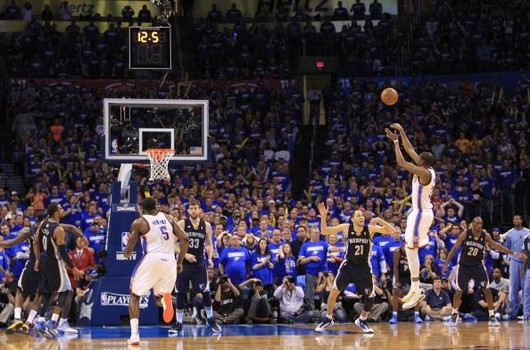
\includegraphics[width = 0.4\textwidth]{img/Triple.jpg}
\end{center}
\end{problem}

\begin{problem} Considera el $K$-homomorfismo $\appl{φ}{K[x,y]}{K[t]}$ con $φ(x) = t^2$ y $φ(t) = t^3$. Decide de manera razonada si φ factoriza por $\quot{K[x,y]}{\gen{x^2-y^2}}$. ¿Y por $\quot{K[x,y]}{\gen{x^3-y^2}}$?

\solution

\doneby{Guille} \inclass

Según se definía en la \fref{prop:FactorizacionHomomorfismo}, φ factoriza por $\quot{R}{I}$ si $I ⊂ \ker φ$, donde $\ker φ = \set{a ∈ R \tq φ(a) = 0}$. En el caso concreto de este ejercicio, lo que tenemos que ver es si $\gen{x^2 - y^2}$ y $\gen{x^3-y^2}$ están dentro de $\ker φ$.

Si $p(x,y) ∈ \gen{x^2-y^2}$, entonces $p(x,y) = a·(x^2-y^2)^n$ para $a ∈ K[x,y]$ y $n ∈ ℕ$. Calculando su imagen por $φ$, tenemos que \[ φ(p) = φ(a) · \left(φ(x^2) - φ(y^2)\right)^n = φ(a) · (t^4 - t^6)^n ≠ 0\], luego $\gen{x^2-y^2} \not\subset \ker φ$ y φ no factoriza por $\quot{K[x,y]}{\gen{x^2-y^2}}$.

Haciendo el proceso análogo con $p ∈ \quot{K[x,y]}{\gen{x^3-y^2}}$, nos saldrá que \[ φ(p) = φ(a) · (t^6 - t^6)^n = 0 \], así que $\gen{x^3-y^2} ⊂ \ker φ$ y $φ$ sí factoriza por $\quot{K[x,y]}{\gen{x^3-y^2}}$.

\end{problem}

\begin{problem}[6] \textbf{Teorema chino del resto}. Sea $R$ un anillo y sean $I_1, \dotsc, I_n$ ideales en $A$. Consideramos el siguiente homomorfismo de anillos:
\begin{align*}
\appl{φ}{R&}{\quot{R}{I_1} × \dotsb \quot{R}{I_n}} \\
r &\longmapsto (r_1, \dotsc, r_n)
\end{align*} donde $r_i$ denota la clase de $r$ módulo $I_i$. Demuestra que:

\ppart φ es sobreyectiva si y sólo si $I_i$ e $I_j$ son primos entre sí cuando $i ≠ j$.
\ppart φ es inyectiva si y sólo si $\bigcap I_i = \zerogen$.

\textit{Sugerencia general: Empieza considerando el caso $n = 2$. Para el primer apartado, en $\implies$ hay que observar que $(1,0)$ y $(0,1)$ tienen preimagen; para $\impliedby$ basta comprobar que $(1,0)$ y $(0,1)$ tienen preimagen. Para el segundo apartado, calcula $\ker φ$.}

\solution

\doneby{Guille}

Recordamos que dos ideales $I,J ⊂ R$ son \concept[Ideal\IS coprimo]{Ideales\IS coprimos} si $I + J = R$.

\spart

Demostrarmos primero la implicación a la derecha: si φ es sobreyectiva, entonces $I_i$ e $I_j$ son primos entre sí cuando $i ≠ j$. Vamos a demostrar que cualquier $a ∈ R$, con $a ∉ I_i, I_j$ se puede expresar como suma de elementos de $I_i$ e $I_j$.

Consideramos la imagen de $a$, $φ(a) = (a_1, \dotsc, a_n)$. Como $a$ no está ni en $I_i$ ni en $I_j$, tiene que ser $a_i, a_j ≠ 0$. Ahora bien, podemos descomponer $φ(a)$ como suma de tres elementos $φ(a) = α + a_i·1_i + a_j · 1_j$, donde $1_i$ es un vector nulo salvo por un $1$ en la coordenada $i$ y $α$ tiene las mismas coordenadas que $φ(a)$ salvo por la $i$-ésima y $j$-ésima, que son nulas.

Como φ es sobreyectiva, todos los sumandos tienen preimágenes. En concreto, la de $α$ está en $I_i ∩ I_j$, y las de $a_i · 1_i$ y $a_j · 1_j$ están en $I_j$ y en $I_i$ respectivamente. Por las propiedades de homomorfismo, la suma de esas preimágenes será igual a $a$, luego efectivamente cualquier $a ∉ I_i, I_j$ se puede expresar como suma de elementos de $I_i$ y $I_j$, por lo que $I_i$ e $I_j$ son primos entre sí.

Para la implicación al otro lado, suponemos que $I_i, I_j$ son coprimos cuando $i ≠ j$, y tratamos de demostrar que $φ$ es sobreyectiva. Como nos dice la sugerencia, nos basta con demostrar que $1_i$ tiene preimagen para $i = 1, \dotsc, n$, ya que sólo con eso podremos construir cualquier elemento en la imagen.

Si $φ(a) = 1_i$, significa que $a ∉ I_i$ pero $a ∈ I_j$ si $i ≠ j$. Si tal $a$ no existe, eso significa que cualquier elemento que esté en todos los $I_j$ con $i ≠ j$ está también en $I_i$. Luego $I_i ⊆ I_j$ para cualquier $j = 1, \dotsc, n$, contradicción porque entonces $I_j + I_j = I_j$ y no serían coprimos.

\spart

Sabemos que $a ∈ \ker φ \iff φ(a) = (0, \dotsc, 0)$, es decir, si y sólo si $a ∈ \bigcap I_i$. En otras palabras, $\ker φ = \bigcap I_i$, y efectivamente ya sabemos que φ es inyectiva si y sólo si $\ker φ = \zerogen$.

\end{problem}

\begin{problem} Demuestra que

\ppart Si $\gcd (n,m) = 1$ entonces $ℤ_{n·m} \simeq ℤ_n × ℤ_m$.
\ppart Demuestra que $\quot{ℝ[x]}{\gen{(x^2-1)x^3}}$ es isomorfo a la suma directa de tres anillos locales, que dos de ellos son un cuerpo y que el tercero tiene nilpotentes.

\solution

\inclass

\spart

Usamos el ejercicio anterior: si $R = ℤ_{nm}$, entonces hay dos ideales $I_1 = \gen{n}, I_2 = \gen{m}$ coprimos, y además $I_1 ∩ I_2 = \zerogen$. Por lo tanto, estamos en las condiciones del ejercicio anterior y el homomorfismo que se definía ahí $\appl{φ}{R}{\quot{R}{I_1} × \quot{R}{I_2}}$ es sobreyectivo e inyectivo, luego es isomorfismo y $ℤ_{n·m} \simeq ℤ_n × ℤ_m$.

\spart

De nuevo usando el ejercicio anterior, vemos que en el anillo $\quot{ℝ[x]}{\gen{(x^2-1)x^3}}$ hay tres ideales, $I_1 = \gen{x-1}$, $I_2 = \gen{x+1}$, $I_3 = \gen{x^3}$, por lo que es isomorfo \[ \quot{ℝ[x]}{\gen{(x^2-1)x^3}} \simeq \quot{ℝ[x]}{\gen{x-1}} × \quot{ℝ[x]}{\gen{x+1}} × \quot{ℝ[x]}{\gen{x^3}} \] donde $\quot{ℝ[x]}{\gen{x\pm 1}} \simeq ℝ$, que es un cuerpo, y en  $\quot{ℝ[x]}{\gen{x^3}}$ hay nilpotentes, tal y como nos pedían.

\end{problem}

\begin{problem} Encuentra ejemplos de anillos que verifiquen las siguientes condiciones:

\ppart Un anillo que tenga exactamente 2 ideales maximales y al menos un nilpotente no nulo.
\ppart Un anillo con un único ideal primo \pideal (por tanto necesariamente maximal) que no sea un cuerpo.

\solution

\inclass

\spart

Los ideales de $\quot{ℝ[x]}{\gen{x^3}}$ no son un misterio porque se corresponden de forma biyectiva con ideales de $ℝ[x]$ que contienen a $\gen{x^3}$. Sólo hay un maximal en $ℝ[x]$ que contenga a $\gen{x^3}$: $\gen{x}$.

Usando la misma idea, podemos coger $\gen{x^2(x-1)}$ que sólo tiene dos factores irreducibles ($x$ y $x-1$).

Otro ejemplo más fácil es $ℤ_{12}$.

\spart



\end{problem}

\begin{problem}[9] \label{ej:Hoja2:9} Demuestra que todo ideal $I \subsetneq R$ está contenido en un primo minimal siguiendo los siguientes pasos:

\begin{enumerate}
\item Considera el conjunto Σ de ideales primos de $R$ que contienen a $I$ y demuestra que no es vacío.
\item Define en Σ el siguiente orden parcial: $\mathfrak{p} ≤ \mathfrak{p}'$ si $\mathfrak{p}' ⊆ \mathfrak{p}$, y demuestra que toda cadena creciente de elementos en Σ tiene una cota superior en Σ.
\item Usa el \nref{lem:Zorn}.
\end{enumerate}

\solution

\doneby{Guille}

Para ver que Σ no es vacío, vemos que el \fref{thm:IdealContenidoMaximal} nos dice que $I$ estará contenido en un maximal, y los ideales maximales son primos, luego esa parte ya la tenemos.

La cota que damos es $\aideal = \bigcap_{\pideal ∈ Σ} \pideal$, que es obvio que contiene a $I$ y es un ideal, luego la cadena está acotada y tiene un elemento maximal por el \nref{lem:Zorn}. Ese elemento maximal será el primo más pequeño que contiene a $I$.
\end{problem}

\begin{problem}[10] \label{ej:Hoja2:10} Sea $I ⊂ R$ un ideal, y sea $M$ el conjunto de los ideales primos que contienen a $I$. Demuestra que \[ \sqrt{I} = \bigcap_{\pideal ∈ M} \pideal \]

\hint{Considera el cociente $\quot{R}{I}$. ¿Qué es $\mop{Nil}(\quot{R}{I})$?}

\solution

\doneby{Guille}

Los elementos nilpotentes en $\quot{R}{I}$ son aquellos para los que existe un cierto $n ∈ ℕ$ con $\cls{a}^n = 0$, o equivalentemente $a^n ∈ I$. Es decir, que $\mop{Nil}(\quot{R}{I}) = \sqrt{I}$.

Ahora usamos la \fref{prop:NilpotentesInterPrimos} que nos dirá que \[ \mop{Nil}\left(\quot{R}{I}\right) = \bigcap_{\substack{\pideal ⊂ \quot{R}{I} \\ \pideal \text{ primo}}} \pideal \] y como hay correspondencia biyectiva entre los ideales de $\quot{R}{I}$ y los ideales de $R$ que contienen a $I$ hemos terminado.

\end{problem}

\begin{problem}[11] \label{ej:Hoja2:11} Utiliza el ejercicio anterior para demostrar que dados dos ideales $I,J ⊂ R$ se tiene que $\sqrt{IJ} = \sqrt{I ∩ J} = \sqrt{I} ∩ \sqrt{J}$. \hint{El \fref{ej:Hoja1:5} puede ser útil.}

\solution

Por la definición del anterior ejercicio vemos que \[ \sqrt{I ∩ J} = \bigcap_{\substack{\pideal ⊂ R \\ I ∩ J ⊂ \pideal \\ \pideal\text{ primo}}} \pideal \]

Ahora bien, si $I ∩ J ⊂\pideal$, según el \fref{ej:Hoja1:5} tenemos que o bien $I ⊂ \pideal$ o bien $J ⊂ \pideal$, y en el otro sentido también lo tenemos ($I ⊂ \pideal$ ó $J ⊂ \pideal$ implica $I ∩ J ⊂ \pideal$) luego podemos separar la intersección en \[
\sqrt{I ∩ J} =
	\bigcap_{\substack{\pideal ⊂ R \\ I ∩ J ⊂ \pideal \\ \pideal\text{ primo}}} \pideal =
	\bigcap_{\substack{\pideal ⊂ R \\ I ⊂ \pideal \\ \pideal\text{ primo}}} \pideal
	∩
	\bigcap_{\substack{\pideal ⊂ R \\ J ⊂ \pideal \\ \pideal\text{ primo}}} \pideal
	= \sqrt{I} ∩ \sqrt{J}
\]
\end{problem}

\subsection{Problemas para entregar}

\begin{problem} Sea $R$ un anillo y sea $\mathfrak{p} ⊂ R$ un ideal primo. Demuestra que $\mathfrak{p}$ contiene un primo minimal, es decir, demuestra que existe un primo $\mathfrak{q} ⊂ \mathfrak{p}$ tal que si $\mathfrak{r} ⊂ R$ es otro ideal primo con $\mathfrak{r} ⊂ \mathfrak{q}$ entonces $\mathfrak{r} = \mathfrak{q}$.

\textup{Sugerencia: Puedes usar una idea parecida a la del \fref{ej:Hoja2:9}}.

\solution
\doneby{Parra}

Utilizaremos el Lema de Zorn: Sea $\Sigma$ un conjunto no vacío parcialmente ordenado. Si toda cadena creciente de elementos de $\Sigma$ tiene una cota superior, entonces $\Sigma$ tiene un elemento maximal.

Definimos el conjunto $\Sigma$ como el conjunto de todos los ideales primos contenidos en $p$, entonces:
\begin{itemize}
	\item $\Sigma \neq \emptyset$ ya que $\pideal \subset \pideal$.
	\item Definimos la siguiente relación: $\pideal \leq \pideal' \Leftrightarrow \pideal' \subset \pideal$.
	\item Sea $L=\{\pideal_i\}$ una cadena creciente de ideales primos, es decir $\pideal_n \leq \pideal_m\; \forall m \geq n$, que dada la relación de equivalencia definida es lo mismo que decir que $\pideal_n \supset \pideal_m\; \forall m \geq n$. Queremos ver que la cadena está acotada en $\Sigma$.

	Podemos coger como cota superior $\pideal_0=\bigcap_{\pideal_i\in L}$. Esta claro que $\pideal_0 \geq \pideal_i\; \forall i$, ya que $\pideal_0 \subset \pideal_i\;  \forall i$.

	Sabemos que la intersección de ideales es un ideal, por tanto, nos falta ver que $p_0$ es primo, es decir, que si tomamos $a,b \in R$ tal que $a\cdot b \in p_0$, entonces $a$ ó $b$ tiene que pertenecer a $\pideal_0$, es decir o $a$ o $b$ pertenecen a todos los $\pideal_i$ de L. Supongamos que no, tenemos dos posibilidades:
	\begin{enumerate}
		\item $a$ y $b$ no pertenecen a ningún $\pideal_i \in L$, entonces ningún $\pideal_i$ es primo, por lo que llegamos a contradicción.
		\item Suponemos que existen $a,b\in R$, tal que $a \in \pideal_i, b \notin \pideal_i$ y $a \notin \pideal_i,\, b \in \pideal_j$ con $j \neq i$. Que también nos llevaría a contradicción ya que, asumimos sin pérdida de generalidad que $\pideal_i \leq \pideal_j$, por tanto $\pideal_j \subset \pideal_i$, por tanto, $a,b \in \pideal_i$.
	\end{enumerate}

	Por tanto, tenemos cota superior, y cumplimos las hipótesis del Lema de Zorn. Lo aplicamos y tenemos que existe un elemento maximal, que es el primo minimal buscado.
\end{itemize}


\end{problem}


\begin{problem} Encuentra todos los primos minimales en

\ppart $ℤ_{12}$
\ppart $ℤ_9[x]$
\ppart $\quot{\K[x]}{\gen{x^3(x-1)}}$
\ppart $\quot{ℝ[x,y]}{\gen{x-y^2}}$.

\solution
\doneby{Parra}

\spart En $\ent_{12}$ tenemos 4 ideales distintos del total o del $\{\zero \}$ que son: $\gen{2}$, $\gen{3}$, $\gen{4}$ y $\gen{6}$. Los dos últimos no son primos ya que tenemos que $2 \cdot 2 \in \gen{4}$ y $2 \notin \gen{4}$. Y por otro lado $2 \cdot 3 \in \gen{6}$ y $2,3 \notin \gen{6}$.

Los únicos primos minimales son $\gen{2}$ y $\gen{3}$

\spart En $\ent_9[x]$ hacemos lo siguiente:

En primer lugar, sabemos que el $\zero$ pertenece a cualquier ideal, incluidos los ideales primos. En $Z_9[x]$ tenemos que $\zero=3\cdot 3$. Por tanto, el $3\in p$ para cualquier primo p. Por tanto $\gen{3} \subset p$ para cualquier primo p.

Ahora, vamos a ver qué es $\gen{3}$ en $\ent_9[x]$. Para ello definimos el anillo cociente:
$$ \quot{\ent_9[x]}{\gen{3}}\simeq\ent_3[x]$$

Pero $\ent_3[x]$ es un dominio de integridad (no es un cuerpo ya que el $x$ no tiene inverso, porque $\frac{1}{x} \notin \ent_3[x]$). Por ser dominio de integridad, entonces $\gen{3}$ es un ideal primo en $\ent_9[x]$.

Por tanto, $\gen{3}$ es el único primo minimal de $\ent_9[x]$

\spart

Queremos aplicar la idea de que sea un homomorfismo $f:R \longmapsto \quot{R}{I}$ tenemos que hay una correspondencia biyectiva entre los ideales primos en $R$ que contengan a $I$ y los ideales primos de $\quot{R}{I}$ (proposición \ref{prop:correspondencia_biyectiva}).

Por tanto tenemos que hay una correspondencia biyectiva entre los ideales primos en $\K[x]$ que contengan a $\gen{x^3(x-1)}$ y los ideales primos de $\quot{\K[x]}{\gen{x^3(x-1)}}$

\textbf{Dos formas parecidas de pensarlo:}
\begin{itemize}
	\item \textbf{Más para este ejemplo en particular:} En este caso, por ser $K$ un cuerpo, los ideales primos en $K[x]$ vienen dados por $\gen{p(x)}$ con $p(x)$ irreducible.

	Los dos únicos polinomios irreducibles que dividen a $x^3(x-1)$ son $x$ y $(x-1)$, por lo tanto, los dos únicos ideales primos que contienen a $\gen{x^3(x-1)}$ en $\K[x]$ son $\gen{x}$ y $\gen{x-1}$.

	Por la correspondencia biyectiva, los dos únicos ideales primos en $\quot{\K[x]}{\gen{x^3(x-1)}}$ son $\gen{x}$ y $\gen{x-1}$, que no se contienen entre ellos y por tanto son los dos primos minimales.

	\item \textbf{Más genérica:} vamos a coger los ideales primos $p \in R$ que contengan al ideal $\gen{x^3(x-1)}$.

	Por tanto, buscamos los ideales primos $p$ tal que el elemento $x^3(x-1) \in p$, entonces, por ser $p$ primo $x \in p$ o $(x-1) \in p$. Eso implica que  $\gen{x} \in p$ o $\gen{x-1} \in p$.

	Ahora vamos a ver qué tipo de ideales son $\gen{x}$ y $\gen{x-1}$

	En este caso, como hemos dicho antes, por ser $K$ un cuerpo, los ideales primos en $K[x]$ vienen dados por $\gen{p(x)}$ con $p(x)$ irreducible.

	En otros casos, para ver qué tipo de ideales definimos su anillo cociente:

	\begin{itemize}
		\item $\quot{K[x]}{\gen{x}} \simeq K$ que es un cuerpo, y por tanto un dominio de integridad. Por tanto $\gen{x}$ es primo y maximal.
		\item $\quot{K[x]}{\gen{x-1}}$.  Igual que el anterior.
	\end{itemize}

	Por tanto, tenemos que tanto $\gen{x}$ como $\gen{x-1}$ son primos en $K[x]$, y ambos contienen a $\gen{x^3(x-1)}$, entonces, por la correspondencia biyectiva. también son primos en $\quot{K[x]}{\gen{x^3(x-1)}}$. Así que $\gen{x}$ como $\gen{x-1}$ son los primos minimales de $\quot{K[x]}{\gen{x^3(x-1)}}$.
\end{itemize}

NOTA: Al ser $K$ un cuerpo, el ideal generado por un número, por ejemplo el $\gen{2}$, no es primo, ya que $2$ es una unidad.

\spart Puesto que $\cls{y}=\cls{x^2}$, entonces

 $$\quot{ℝ[x,y]}{\gen{x-y^2}} \simeq \real[y]$$

 Pero $\real[y]$ es un dominio de integridad, por tanto $\{0\}$ es ideal primo y por tanto $\{0\}$ es un ideal primo minimal.

\end{problem}

\begin{problem} Sea $\appl{f}{R}{T}$ un homomorfismo de anillos.

\ppart Demuestra que si $J ⊂ T$ es un ideal entonces $\inv{f}(J) = \set{r ∈ R \tq f(r) ∈ J}$ es un ideal en $ℝ$. Demuestra que necesariamente $\ker f  ⊂ \inv{f}(J)$.
\ppart Demuestra que si $I ⊂ R$ es un ideal, entonces $f(I) = \set{f(r) \tq r ∈ I}$ en general no es un ideal en $T$.
\ppart Demuestra que si $I ⊂ R$ es un ideal y $f$ es sobreyectiva entonces $f(I)$ es un ideal en $T$.

\ppart Sea $I ⊂ R$ un ideal. Aunque en general $f(I)$ no tiene por qué ser un ideal en $T$, podemos considerar el ideal que genera en $T$. Denotaremos por $I^e$ al ideal generado por $f(I)$ en $T$.  Demuestra que $I ⊂ \inv{f}(I^e)$ y que en general el contenido es estricto.
\ppart Sea $J ⊂ T$ un ideal. Demuestra que $(\inv{f}(J))^e ⊂ J$ y que en general el contenido es estricto.

\solution

\doneby{Guille}

\spart

Vamos a demostrar que es un ideal. Sabemos que no es vacío ya que $f(0) = 0$ y $0 ∈ J$ por ser ideal, luego $0 ∈ \inv{f}(J)$. La propiedad de absorción también se cumple: si $r ∈ R$ y $a ∈ \inv{f}(J)$, tenemos que $f(ra) = f(r)·f(a) ∈ J$ por la absorción de $J$, ya que $f(a) ∈ J$. Por último, queremos ver que si $a, b ∈ \inv{f}(J)$ entonces $a + b ∈ \inv{f}(J)$, que también se cumprueba fácilmente: $f(a+b) = f(a) + f(b) ∈ J$ por ser ser $J$ ideal.

Para la segunda proposición, si $a ∈ \ker f$ entonces $f(a) = 0 ∈ J$, por lo que $a ∈ \inv{f}(J)$.

\spart

Si tomamos la inclusión $\appl{i}{ℤ}{ℚ}$ e $I = \gen{2} ⊂ ℤ$, éste es un ideal en $ℤ$ pero $i(\gen{2}) ⊂ ℚ$ no lo es en $ℚ$, ya que no se cumpliría la propiedad de absorción.

\spart

Vamos a comprobarlo. Esta claro que $f(I)$ no será vacío si $I$ no lo es. Comprobamos la propiedad de absorción: sea $t ∈ T$ y $a ∈ f(I)$, con $a = f(b)$ y $b ∈ I$. Dado que $f$ es sobreyectiva, existe al menos un $r ∈ R$ tal que $f(r) = t$. Entonces podemos operar y ver que \[ t · a = f(r) · f(b) = f(r·b) ∈ f(I) \] ya que $r·b ∈ I$ por absorción de $I$.

Por último, queremos ver que si $a,b ∈ f(I)$, entonces $a+ b ∈ f(I)$. Denotamos $a = f(c), b = f(d)$ con $c,d ∈ I$ y entonces \[ a + b = f(c) + f(d) = f(c+d) ∈ f(I) \] ya que $c + d ∈ I$ igualmente.

\spart

Podemos ver que \[ \inv{f}(f(I)^e) = \set{r ∈ R \tq f(r) ∈ f(I)^e} \] o, en otras palabras, $r ∈ \inv{f}(f(I)^e)$ si y sólo si \[ f(r) = α_1 f(β_1) + \dotsb + α_n f(β_n)\] para unos ciertos $α_i ∈ T$ y $β_i ∈ I$. En concreto, si $r ∈ I$ simplemente podemos tomar $α_1 = 1 ∈ T$ y $β_1 = r ∈ I$, por lo que efectivamente $r ∈ I \implies r ∈ \inv{f}(f(I)^e)$.

Para demostrar que el contenido en general es estricto, vemos el ejemplo del apartado $B$: si tomamos la inclusión $\appl{i}{ℤ}{ℚ}$ e $I = \gen{2} ⊂ Z$, podemos ver que $3 = \frac{3}{2} · 2∈ f(I)^e$, pero $\inv{f}(3) = 3 ∉ \gen{2}$.

\spart

Por definición, $j ∈ (\inv{f}(J))^e$ si y sólo si existen unos ciertos $\set{t_i}_{i=1}^n ⊂ T$, $\set{r_i}_{i=1}^n ⊂ \inv{f}(J)$ tales que $j = t_1 f(r_1) + \dotsb + t_n f(r_n)$.

Ahora bien, $f(r_i) ∈ J$, por absorción sabremos que $t_i f(r_i) ∈ J$ y por lo tanto $j ∈ J$, así que efectivamente $(\inv{f}(J))^e ⊆ J$.

Para ver que el contenido en general es estricto... \noteby{Guille}{Ni idea de esto.}
\end{problem}

\begin{problem} Trabajamos en $ℝ[x,y]$. Sean $a,b ∈ ℝ$. ¿Cuál es la condición necesaria y suficiente para que un maximal de la forma $\gen{x-a, y-b}$ contenga al ideal $\gen{x-y^2}$?


\textup{Sugerencia: $\gen{x-y^2} ⊂ \gen{x-a, y-b}$ si y sólo si el homomorfismo del paso al cociente $ℝ[x,y] \mapsto \quot{ℝ[x,y]}{\gen{x-a, y-b}} \simeq ℝ$ factoriza por $\quot{ℝ[x,y]}{\gen{x-y^2}}$. ¿Por qué? Y ahora piensa, ¿cuál es el homomorfismo composición $ℝ[x,y] \mapsto ℝ$?}

\solution

\inclass

Una condición necesaria y suficiente para que $\gen{x-a, y-b} ⊂ K[x,y]$ sea maximal es que $K$ sea un cuerpo. Vamos ahora al ejercicio.

Lo primero es comprobar que $\gen{x-y^2}$ sea maximal. La respuesta es que no: $\quot{ℝ[x,y]}{x-y^2} \simeq ℝ[y]$, que no es un cuerpo luego $\gen{x-y^2}$ no es maximal. Lo que sí es es primo, ya que $ℝ[y]$ no tiene divisores de cero.

Una observación es ver que $\gen{x-y^2} ⊂ \gen{x-a, y-b}$ si y sólo si $\gen{x-a, y-b}$ es de los maximales de $ℝ[x,y]$ que están en correspondencia biyectiva con los maximales de $\quot{ℝ[x,y]}{\gen{x-y^2}}$. Ahora vamos a tratar de construir un $ℝ$-homomorfismo decidiendo a dónde mandamos a $x$ e $y$. En concreto, lo definiremos de la siguiente forma:
\begin{align*}
\appl{f}{ℝ[x,y]&}{ℝ} \\
x &\longmapsto a \\
y &\longmapsto b
\end{align*}

Aunque no lo pide el problema, podemos ver que $\ker f = \gen{x-a, y-b}$. El contenido obvio es que $\gen{x-a, y-b} ⊂ \ker f$, aunque para la inclusión al otro lado hay que pensar algo más. Como $\gen{x-a,y-b}$ es maximal, si $\ker f ≠ \gen{x-a, y-b}$ tendría que ser $\ker f = ℝ[x,y]$, pero eso no es un homomorfismo.

Volvemos otra vez al problema. Y tenemos que girar la ficha del puzzle o, en otras palabras tenemos que hacer que el diagrama de la \fref{fig:Teorema1Isomorfia:Diag1} conmute o, equivalentemente, que $f = f' ○ π$. Esto ocurrirá sólo si $a = b^2$, y esta es la condición que buscábamos

\begin{figure}
\centering
\begin{tikzpicture}[scale = 1.5]
\node (A) at (0,0) {$ℝ[x,y]$};
\node (B) at (4,0) {$\quot{ℝ[x,y]}{\gen{x-a,y-b}}$};
\node (C) at (2,-2) {$\quot{ℝ[x,y]}{\gen{x-y^2}}$};

\draw[->] (A) -- node[midway, above, align = center] {\footnotesize $x \to a$ \\ \footnotesize $y \to b$} node[midway, below] {$f$} (B);
\draw[->] (A) -- node[midway, below, sloped, align = center] {\footnotesize $x \to y^2$ \\ \footnotesize $y \to y$} node[midway, above, sloped] {$π$} (C);
\draw[->] (B) -- node[midway, below, sloped, align = center] {\footnotesize $y^2 \to a$ \\ \footnotesize $y \to b$} node[midway, above, sloped] {$f'$} (C);
\end{tikzpicture}
\caption{Diagrama que queremos hacer conmutativo}
\label{fig:EjHoja2:13}
\end{figure}

\end{problem}

\begin{problem} Demuestra que el ideal $\gen{x^2 + x - y} ⊂ ℝ[x,y]$ es primo. ¿Es maximal?

\solution

\doneby{Parra}

Tenemos que $\cls{x^2+x}= \cls{y}$.

Definimos la aplicación:
$$f:\real[x] \longmapsto \quot{ℝ[x,y]}{\gen{x^2+x-y}}$$

Es sobreyectiva ya que sea un $p(x,y) \in \real[x,y]$ cualquiera, se puede escribir como un $p(x) in \real[x]$.

Además también es inyectiva ya que $\ker(f)=\{p(x):\cls{p(x)}=0 \}$. Esos son los $p(x) \in \gen{x^2+x-y}$. Sea $p(x) \in \gen{x^2+x-y}$ en $\real[x,y]$, entonces $\exists q(x,y) \in \real[x,y]$ tal que $p(x)=q(x,y)(x^2+x-y)$. Lo cual solo es posible si $q(x,y)=0$, que implica que $p(x)=0$ y por tanto $\ker(f)=0$.

Así nos queda que:

$$\quot{ℝ[x,y]}{\gen{x^2+x-y}} \simeq \real[x]$$

Como $\real[x]$ es un dominio de integridad, entonces $\gen{x^2+x-y}$ es primo. Pero $\real[x]$ no es un cuerpo, ya que $x$ no tiene inverso multiplicativo porque $\frac{1}{x} \notin \real[x]$, por tanto, no es maximal.

\end{problem}

\section{Hoja 3: Módulos, localización}

\begin{problem} Sea $\appl{f}{R}{S}$ un homomorfismo de anillos y sea $N$ un $S$-módulo. Demuestra que, vía $f$, $N$ es de manera natural un $R$-módulo. En particular, observa que todo ideal de $S$ es un $R$-módulo, y que $S$ es un $R$-módulo.

\solution

\doneby{Guille}

La definición para que $N$ sea un $R$-módulo es clara: si φ es la operación externa $\appl{φ}{S×N}{N}$, entonces podemos definir otra operación externa para $N$ sobre $R$ de la siguiente forma: \begin{align*}
\appl{γ}{R × N&}{N} \\
(r,n) &\longmapsto φ(f(r), n)
\end{align*} cuyas propiedades sensatas se pueden calcular con facilidad, ya que van a venir dadas o bien porque las cumple φ o porque $f$ es homomorfismo. Vamos a ir una por una:

\begin{itemize}
\item $∀r ∈ R,\,∀n,n' ∈ N$ se cumple $γ(r, n + n') = φ(f(r), n + n') = φ(f(r), n) + φ(f(r), n') = γ(r,n) + γ(r,n')$, ya que $φ$ es la operación externa de $N$ como $S$-módulo.
\item $∀r,r' ∈ R,\, ∀n ∈ N$ tenemos que $γ(r+r',n) = φ(f(r+r'), n) = φ(f(r) + f(r'), n) = γ(r, n) + γ(r',n)$.
\item Del resto de propiedades ya paso porque salen igual, nos podemos hacer todos a la idea.
\end{itemize}

En clase habíamos visto que los ideales $I ⊂ S$ son $S$-módulos, por lo que dada la construcción que acabamos de hacer, también serán $R$-módulos. Como $S$ es un ideal de $S$, igualmente será un $R$-módulo.

\end{problem}

\begin{problem} Sea $R$ un anillo. Demuestra que $R[x_1, \dotsc, x_n]$ no es un $R$-módulo finitamente generado. Demuestra que en cambio es una $R$-álgebra finitamente generada. ¿Es $ℚ[\sqrt[3]{2}]$ una $ℚ$-álgebra finitamente generada? ¿Es $ℚ[\sqrt[3]{2}]$ un $ℚ$-módulo finitamente generado?

\solution

\doneby{Guille}

$R[x_1, \dotsc, x_n]$ no puede ser finitamente generado como $R$-módulo, ya que con combinaciones lineales no podemos poner cualquier $x_j^k$. Si está finitamente generada como $R$-álgebra, con $x_1, \dotsc, x_n$ los generadores.

$ℚ[\sqrt[3]{2}]$ es un $ℚ$-módulo finitamente generado con generadores $\set{1, \sqrt[3]{2}, \sqrt[3]{2^2}}$, y por lo tanto también es una $ℚ$-álgebra finitamente generada.

\end{problem}

\begin{problem} Sean $M$ y $N$ dos $R$-módulos.

\ppart Demustra que el conjunto de los homomorfismos de $R$-módulos de $M$ en $N$, $\mop{Hom}_R (M,N)$ es un $R$-módulo.

\ppart Considera la aplicación \begin{align*}
\appl{φ}{R&}{\mop{Hom}_R(M,M) = \mop{End}_R M} \\
r & \longmapsto f_r \end{align*} donde $f_r(m) = rm$. Demuestra que $φ$ es un homomorfismo de $R$-módulos, y que $\quot{R}{\mop{Ann}_R(M)} ⊂ \mop{End}_R(M)$, donde \[ \mop{Ann}_R(M) ≝ \set{a ∈ R \tq am = 0\;∀m ∈ M}\] es un ideal de $R$.

\solution

\doneby{Guille} \inclass

\spart

Por comodidad, voy a denotar $H = \mop{Hom}_R (M,N)$. La operación externa la vamos a definir de la siguiente forma: dados $r ∈ R$ y $f ∈ H$, entonces $(r,f) \mapsto r·f ∈ H$. Así, podemos verificar las propiedades:

\begin{itemize}
\item No es vacío: el homomorfismo $f(m) = 0$ que envía todo a cero siempre está en $H$.
\item $H$ es un grupo abeliano, ya que $(f+g)(m) = f(m) + g(m) = g(m) + f(m) = (g + f) (m)$.
\item $∀ r ∈ R,\,∀f,g ∈ H$ tenemos que ver cuánto vale $r · (f + g)$. Para calcularlo, aplicamos este homomorfismo a un elemento $m ∈ M$, y entonces \[ (r · (f+g))(m) = r · (f+g) (m) = r·f(m) + r·g(m) \], luego efectivamente se cumple si aceptamos que $(f+g)(m) = f(m) + g(m)$.
\item Análogamente.
\end{itemize}

Esto puede ser útil cuando tomamos $J,I ⊂ R$ ideales de $R$. Por ejemplo, si tomamos $r ∈ (I:J)$ (el conductor) tenemos $R$-homomorfismos. Lo interesante de este tipo de homomorfismo es algo. Otro caso curioso es cuando tenemos homomorfismos de $J$ en sí mismo, que puede ser una herramienta computacional para cosas.

\spart

La demostración de las propiedades de homomorfismo es trivial.

Para lo otro, vemos que $\ker φ = \set{r ∈ R \tq φ(r) = f_r = f_0}$, luego $\ker φ = \mop{Ann}_R (M)$. Entonces podemos usar los teoremas de isomorfía\footnoteby{Guille}{No estoy seguro de que se use esto.} y entonces hay una inclusión $\quot{R}{\mop{Ann}_R(M)} ⊂ \mop{End}_R(M)$.

\end{problem}

\begin{problem} Sea $I = \gen{\cls{2}} ⊂ ℤ_6$. Demuestra que $I$ es también un $ℤ_3$-módulo.

\solution

\inclass

Aplicamos lo que hemos visto en el ejercicio anterior, con $R = ℤ_6$ y $M = I$, y consideramos los endomorfismos $\mop{End}_{ℤ_6} (\gen{\cls{2}})$. Ahora calculamos y vemos que \[ \mop{Ann}_{ℤ_6} \gen{\cls{2}} = \gen{\cls{3}}\] y algo que me he perdido.

\end{problem}

\begin{problem} Sea $R$ un anillo y sea $\mathfrak{m} ⊂ R$ un ideal maximal. Demuestra que $\quot{\mathfrak{m}}{\mathfrak{m}^2}$ es un $R/\mathfrak{m}$-espacio vectorial.

\solution

\doneby{Guille}

Voy a usar algo que no tengo muy claro que vaya a funcionar, pero bueno: un espacio vectorial es un $R$-módulo con $R$ cuerpo. Luego miro a ver qué se puede hacer con esto.

\end{problem}

\begin{problem} Sea $S = \set{\cls{1}, \cls{2}} ⊂ ℤ_4$. Describe $\inv{S}ℤ_4$.

\solution

\doneby{Guille}

Tenemos que $\inv{S} ℤ_4$ es $\set{0}$ (haciendo las cuentas se ve que todas las posibles fracciones son equivalentes y equivalentes al $0$).

\end{problem}

\begin{problem} Sea $R$ un anillo, y supongamos que $S ⊂ R$ es un conjunto multiplicativamente cerrado que contiene un elemento nilpotente. ¿Qué podemos decir de $\inv{S} R$?

\solution

\doneby{Guille}

Si $S$ contiene nilpotentes, entonces $\inv{S}R$ es cero. Para demostrarlo vemos que, si $S$ es multiplicativamente cerrado y $a ∈ S$ es nilpotente, entonces $a^k ∈ S$ para cualquier $k$, así que en particular $0 ∈ S$. Eso implica que $\frac{0}{0} ∈ \inv{S} R$, y es fácil ver que cualquier otro elemento que podamos construir es equivalente al $\frac{0}{0}$, luego $\inv{S} R = \set{0}$.

\end{problem}

\begin{problem} Sea $R$ un anillo y sea $\pideal ⊂ R$ un ideal primo. Demuestra que $R_\pideal$ es un \nlref{def:AnilloLocal} con ideal maximal $\pideal R_\pideal$.

\solution

\doneby{Guille}

Recordamos que $\pideal R_\pideal$ se define de la siguiente forma: \[ \pideal R_\pideal = \set{ \frac{r}{s} · \frac{p}{1} \tq \frac{r}{s} ∈ R_\pideal,\, p ∈ \pideal } \]

Es obvio ver que es un ideal primo. Supongamos que existen $\frac{r}{s}, \frac{r'}{s'} ∈ R_\pideal$ con $\frac{rr'}{ss'} ∈ \pideal R_\pideal$. En ese caso ha de ser forzosamente $rr' ∈ \pideal$, pero $\pideal$ es primo luego $r, r' ∈ \pideal$ y entonces $\frac{r}{s}, \frac{r'}{s'} ∈ \pideal R_\pideal$.

Para ver que es maximal, suponemos que existe otro ideal $\aideal$ con $\pideal R_\pideal \subsetneq \aideal ⊂ R_\pideal$, y tomamos $\frac{r}{s} ∈ \aideal \setminus \pideal R\pideal $ y $\frac{p}{1} ∈ \pideal R_\pideal$ con $p ∈ \pideal$. En ese caso vemos que $\frac{r}{s}·\frac{p}{1} ∈ \pideal R_\pideal$ por definición, y tenemos que $\frac{r}{s} ∈ \pideal R_\pideal$ por ser éste primo, contradicción.

\end{problem}

\subsection{Problemas para entregar}
\begin{problem}[1]
	Sea $M$ un $R$-módulo y sea $\mop{Ann}_R(M) ≝ \set{a \in R \tq  am = 0, \forall m \in M}$

	\ppart Demuestra que $\mop{Ann}_R(M)$ es un ideal

	\ppart Demuestra que $M$ tiene estructura de $R/\mop{Ann}_R(M)$-módulo y que ésta coincide con la que tiene como $R$-módulo.

	\ppart Considera el ideal $J = \gen{\cls{3}} \subset \ent_{12}$. Demuestra que $J$ es un $\ent_4$-módulo.

	\ppart Decide de manera razonada para qué valores de $n$, el ideal $J$ del apartado anterior es manera natural un $\ent_n$-módulo.

	\solution

	\spart
	\begin{itemize}
		\item $\mop{Ann}_R(M) \neq \emptyset$, ya que $0 \in \mop{Ann}_R(M)$, porque $0\cdot m = 0 \quad \forall m \in M$.
		\item Sea $a \in \mop{Ann}_R(M)$ y $b \in \mop{Ann}_R(M)$ entonces $a+b \in \mop{Ann}_R(M)$.

		Es cierto ya que si $am=0$ y $bm=0$ $\forall m \in M$, entonces por las propiedades sensatas de los $R$-módulos* podemos ver que $(a+b)m=am+bm=0+0=0$.
		\item Sea $a \in \mop{Ann}_R(M)$ y $r\in R$ entonces $(r\cdot a)m=0$ $\forall m \in M$.

		Cierto ya que si $a \in \mop{Ann}_R(M)$ entonces $am=0$, y por las propiedades sensatas de los $R$-módulos tenemos que:
		$r(r'm)=(rr')m \; \forall r,r' \in R, \; \forall m \in M$. Por tanto: $(ra)m=r(am)=r0=0$.
	\end{itemize}

	\spart

	Queremos ver primero que $M$ es un $\quot{R}{\mop{Ann}_R(M)}$-módulo:
	\begin{enumerate}
		\item $(M,+)$ es un grupo abeliano por ser $M$ un $R$-módulo.
		\item  Definimos la operación externa:
		\begin{align*}
			\quot{R}{\mop{Ann}_R(M)} × M & \longmapsto  M \\
			(\cls{r},m) & \longmapsto  \cls{r}\cdot m = rm \\
		\end{align*}
		Tenemos que ver que esta operacion está bien definida. Cogemos un representante de $\quot{R}{\mop{Ann}_R(M)}$, por ejemplo $\cls{r}=r+a$ con $a\in \mop{Ann}_R(M)$. Ahora definimos el producto:

		$$\cls{r} m = (r+a)m= rm+am \underbrace{=}_{a \in \mop{Ann}_R(M)} rm + 0 = rm$$

		Por tanto la operación no depende del representante escogido y la operación esta bien definida. Trivialmente se cumplen las propiedades sensatas.
	\end{enumerate}

	La estructura de $R$-módulo se define la operación externa de la misma forma:

	\begin{align*}
		R × M & \longmapsto  M \\
		(r,m) & \longmapsto  r\cdot m = rm \\
	\end{align*}

	Por tanto $M$ tiene estructura de  $\quot{R}{\mop{Ann}_R(M)}$-módulo y también de $R$-módulo, y estas coinciden. \textcolor{blue}{Las propiedades romanas se cumplen tanto para $M$ como para el cociente, por lo cumplen para $M$ como $R$-módulo. No hace falta probarlo pero hay que decirlo.}

	\spart

	\textcolor{blue}{Basta observar que $\mop{Ann}_{ℤ_{12}} J = \gen{4}$, luego $\quot{\quot{ℤ}{12}}{\quot{4}{12}} \simeq ℤ_4$.} ¿?

	Vamos a probar las dos propiedades:
	\begin{itemize}
		\item $(J,+)$ es un grupo abeliano. Cierto.
		\item  Sea $J=\gen{\cls{3}}=\{ \cls{0}, \cls{3}, \cls{6}, \cls{9} \}$. Definimos la operación externa:
		\begin{align*}
		\ent_4 × J & \longmapsto  J \\
		(\cls{a},\cls{m}) & \longmapsto  \cls{a}\cdot \cls{m} =\cls{a\cdot m} \\
		\end{align*}

		Vamos a ver que este producto está bien definido, es decir, que no depende de los representantes escogidos: $\cls{a}=a+4l$, y $\cls{m}=3n+12k$. Operamos:
		$$\cls{a}\cdot \cls{m}=a3n+12ak+12ln+48lk \eqreasonup[\equiv]{$\mod 12$} a3n=\cls{a3n}=\cls{a}\cls{3n}$$

		Vemos que efectivamente esta operación no depende de los representantes obtenidos y por tanto está bien definida.

		Las propiedades sensatas se cumplen trivialmente \textcolor{blue}{porque se cumplen para $J$ como $ℤ_{12}$-módulo y la estructura de $ℤ_4$-módulo la hereda. También se puede usar el apartado anterior: $\mop{Ann}_{ℤ_{12}} = \gen{\cls{4}}$, luego es un $ℤ_4$-módulo.}
	\end{itemize}

	\spart Para $n=4t \quad \forall t \in \nat$.

	\begin{align*}
	\ent_{4t} × J & \longmapsto  J \\
	(\cls{a},\cls{m}) & \longmapsto  \cls{a}\cdot \cls{m} =\cls{a\cdot m} \\
	\end{align*}

	Vamos a ver que este producto está bien definido, es decir, que no depende de los representantes escogidos: $\cls{a}=a+4tl$, y $\cls{m}=3n+12k$. Operamos:
	$$\cls{a}\cdot \cls{m}=a3n+12ak+12tln+48tlk \underbrace{\equiv}_{mod 12} a3n=\cls{a3n}=\cls{a}\cls{3n}$$

\end{problem}

\begin{problem}
	Sea $R=K[x,y]/\gen{xy}$ y sea $\appl{f}{R}{R_{\gen{x}}}$ el homomorfismo de paso al localizado.

	\ppart Describe $S =R \setminus \gen{x}$

	\ppart A la vista del apartado anterior, ¿qué elementos $a \in R$ serán invertibles vía $f$?

	\ppart Calcula $\ker f$.

	\ppart Utiliza los apartados anteriores y la propiedad universal de la localización para demostrar que ${R_{\gen{x}} \simeq K(y)}$.

	\solution

	\spart

	$R \setminus \gen{x}$ son los elementos de $R$ que no son múltiplos de $x$.

	\spart

	Los elementos invertibles será los $p(x,y) ∈ R\setminus \gen{x}$, es decir, los polinomios que no son múltiplos de $x$.

	\spart

	Sabemos que, dado $a ∈ R$, $f(a) = 0 \iff ∃s ∈ S \setminus \gen{x}$ tal que $s · a = 0$. Si $a ∈ \gen{x}$, entonces podemos encontrar un polinomio $p ∈ S$ con variables sólo en $y$ de tal forma que $a·p ∈ \gen{xy}$. Por otra parte, si $a ∉ \gen{x}$, entonces no es múltiplo de $x$, y si lo multiplicamos por cualquier elemento $s ∈ S$ $a·s$ no va a ser divisible por $xy$, ya que ni $a$ ni $s$ lo son.

	En definitiva, $\ker f = \gen{x}$.

	\spart

\end{problem}

\begin{problem}
	Sea $R$ un anillo, sea $I \subset R$ un ideal y sea $S \subset R$ un subconjunto multiplicativamente cerrado. Considera el homomorfismo de paso al cociente $\appl{\pi}{R}{R/I}$.

	\ppart Demuestra que $\pi(S)$ es un conjunto multiplicativamente cerrado en $R/I$.

	\ppart Demuestra que da lo mismo primero localizar y después cocientar, que primero cocientar y luego localizar. Es decir, demuestra que $S^{-1}R/IS^{-1}R \simeq \pi(S)^{-1}(R/I)$.

	\textit{Sugerencia: considera el siguiente diagrama y utiliza la la propiedad universal para probar que hay un homomorfismo (sobreyectivo) de $S^{-1}R$ en $\pi(S)^{-1}(R/I)$ de modo que el diagrama conmute. Y ahora usa el Primer Teorema de Isomorfía.}

	% http://tex.stackexchange.com/questions/45741/commutative-diagrams-and-tikz
	\begin{large}
	\begin{center}
	\begin{tikzpicture}
	    % set up the nodes
	    \node (R) at (0,0) {$R$};
	    \node[right=of R] (RI) {$R/I$};
	    \node[below=of RI] (SR) {$S^{-1}R$};
	    \node[right=of RI] (piSRI) {$\pi(S)^{-1}(R/I)$};
	    % draw arrows and text between them
	    \draw[->] (R)--(RI) node [midway,above] {$\pi$};
	    \draw[->] (R)--(SR) node [midway,below,sloped] {$f$};
	    \draw[->] (RI)-- node[midway, above] {$γ$} (piSRI);
	    \draw[->] (R) to[bend left=45] node[midway, above] {$φ$} (piSRI.north west);

	    \draw[->] (SR) --node[midway, below, sloped] {$g$} (piSRI.south west);
	\end{tikzpicture}
	\end{center}
	\end{large}

	\ppart Demuestra de otro modo el resultado obtenido en 2c, ahora usando el apartado 3b.

	\textit{Sugerencia: puede que te resulte útil el ejercicio 8.}

	\solution

	\spart

	Para ver que $\cls{1} ∈ π(S)$, simplemente hay que ver que $1 ∈ S$ por ser éste parte mulitplicativa, y entonces $π(1) = \cls{1} ∈ π(S)$.

	Sólo falta ver que dados $\cls{s}, \cls{s'} ∈ π(S)$, entonces $\cls{s}·\cls{s'} ∈ π(S)$. Pero $\cls{s}·\cls{s'} = \cls{s·s'}$, y como $S$ es parte multiplicativa, $ss' ∈ S$, y además ha de ser $π(ss') = \cls{s·s'}$, por lo que efectivamente es conjunto multiplicativamente cerrado.

	\spart

	La propiedad universal de la localización nos dice que si $\appl{φ}{R}{B}$ es un homomorfismo de anillos que lleva elementos de $S ⊂ R$ a unidades en $B$, entonces existe un único homomorfismo de anillos $\appl{g}{S^{-1}R}{B}$ tal que $φ = g ○ f$, con $f$ el homomorfismo de paso al localizado $f(a) = \frac{a}{1}$.

	En nuestro caso, si $\appl{γ}{\quot{R}{I}}{\pi(S)^{-1}(R/I)}$ es el homomorfismo de paso al localizado $\pi(S)^{-1}(R/I)$, entonces la aplicación $\appl{φ = γ ○ π}{R}{\pi(S)^{-1}(R/I)}$ es un homomorfismo de anillos por ser composición de homomorfismos. Vamos a comprobar qué ocurre con los elementos de $s$.

	Si $s ∈ S$, entonces $φ(s) = \frac{\cls{s}}{1}$. Queremos ver que su inverso, que debería ser el elemento $\frac{1}{\cls{s}}$, existe en $π(S)^{-1} (\quot{R}{I})$. Pero el localizado se construye como $\quot{R}{I} × π(S)$ con una relación de equivalencia, y está claro que $\cls{1} ⊂ \quot{R}{I}$ y $\cls{s} ∈ π(S)$, luego $φ(s)$ es invertible.

	Así, podemos aplicar la propiedad universal y ver que existe un único homomorfismo de anillos $\appl{g}{S^{-1}R}{\pi(S)^{-1}(R/I)}$ que hace conmutar el diagrama.

	Tenemos que demostrar que $g$ es sobreyectivo. Afirmamos que la preimagen de un elemento $\frac{\cls{r}}{\cls{s}}$ es $\frac{r}{s}$, y vamos a demostrarlo. Lo primero es ver que $\frac{r}{s} = \frac{r}{1} · \frac{1}{s}$, y como $g$ es homomorfismo podemos simplemente sacar las preimágenes por separado.

	Consideramos $r ∈ R$. Entonces tenemos que \begin{align*}
	(γ ○ π) (r) &= (g○f)(r) \\
	γ(π(r)) &= g(f(r)) \\
	γ(\cls{r}) &= g\left(\frac{r}{1}\right) \\
	\frac{\cls{r}}{\cls{1}} &= g\left(\frac{r}{1}\right)
	\end{align*} así que, tal y como necesitábamos, $g(\frac{r}{1}) = \frac{\cls{r}}{\cls{1}}$. Ahora nos falta ver el análogo para elementos de la forma $\frac{1}{s}$.

	En este caso simplemente tenemos que operar y ver que, por ser $g$ homomorfismo de anillos, \[ \frac{\cls{1}}{\cls{1}} = g\left(\frac{1}{1}\right) = g\left(\frac{s}{1}·\frac{1}{s}\right) = g\left(\frac{s}{1}\right) · g\left(\frac{1}{s}\right) = \frac{\cls{s}}{\cls{1}} · g\left(\frac{1}{s}\right)  \]

	Dado que el inverso es único, $g(\frac{1}{s})$ sólo puede ser $\frac{\cls{1}}{\cls{s}}$. Con esto vemos que \( g\left(\frac{r}{s}\right) = g\left(\frac{r}{1}·\frac{1}{s}\right) = \frac{\cls{r}}{\cls{1}} · \frac{\cls{1}}{\cls{s}} = \frac{\cls{r}}{\cls{s}} \label{eq:H3:DefHomoG} \)

	Esto nos permite dar la preimagen de cualquier $\frac{\cls{r}}{\cls{s}} ∈ \pi(S)^{-1}(R/I)$, luego $g$ es sobreyectiva.

	Ahora afirmamos que $\ker g = IS^{-1}R$, es decir, el ideal generado por $f(I) ⊂ \inv{S}R$. La idea es que si tenemos un elemento $\frac{r}{1} ∈ f(I)$, con $r ∈ I$, éste va a ser preimagen por $f$ de $r ∈ I ⊂ R$. Yendo por el otro lado del diagrama, vemos que $π(r) = 0$ y por lo tanto $φ(r) = \cls{0} ∈ π(S)^{-1} \quot{R}{I}$. Así, la única posibilidad es que $g(\frac{r}{1}) = \cls{0} ∈ π(S)^{-1}$. Por las propiedades de homomorfismos, los elementos de $f(I)^e$ estarán igualmente en $\ker g$.

	Por otra parte, tenemos que ver que si $\frac{r}{s} ∉ IS^{-1}R$ entonces $g(\frac{r}{s}) ≠ 0$. Pero teniendo en cuenta la definición de $g$ de \eqref{eq:H3:DefHomoG}, la única forma es que $r ∈ I$, luego $\frac{r}{s} ∈ IS^{-1}R$, contradicción.

	Finalmente, aplicamos el primer teorema de isomorfía y nos queda lo que queríamos demostrar:
	\begin{align*}
	\quot{S^{-1}R}{\ker g} &\simeq \img g \\
	\quot{S^{-1}R}{IS^{-1}R} &\simeq \pi(S)^{-1}(R/I)
	\end{align*}

	\spart

\end{problem}



\begin{problem}
	Sean $\mathfrak{q}\subset \mathfrak{p}$ dos ideales primos. Demuestra que los ideales primos de $R_\mathfrak{p}/\mathfrak{q}R_\mathfrak{p}$ están en correspondencia biyectiva con los ideales de $R$ que están contenidos en $\mathfrak{p}$ y que contienen a $\mathfrak{q}$.


	\solution

	Escribimos cada elemento para entender mejor el problema:

	$R_p = \{S^{-1}R $ con $ S=R \setminus p \} = \{\frac{r}{s}$, $r \in R$, $s \in R\setminus p \}$ , es decir, hacemos invertibles los elementos de $p$ complementario.

	$qR_p = \{ \varphi(q)^e\subset R_p$ con $\varphi : R \rightarrow S^{-1}R\} = \{\frac{r}{s} \in R_p$ tales que $\frac{r}{s} = \sum^N_{i=0} \frac{r'_i}{s'_i} \frac{q_i}{1}$, $q_i\in q$, $\frac{r'_i}{s'_i}\in R_p\}$

	Es claro que $qR_p \subset R_p$ y por tanto $R_p/qR_p$ será el conjunto que elimina las fracciones cuyos numeradores son generados por $q$.

	Hemos visto en teoría que los ideales del paso al localizado ($\varphi$) quedan invariantes (correspondencia biyectiva) a menos que tengan elementos comunes con $S$, si un ideal contiene un elemento en $S$, al pasar al localizado este elemento se vuelve invertible y por tanto unidad, con lo que la imagen por $\varphi$ extendida será el total ($\varphi(S)^e = S^{-1}R$). También vimos que ideales primos en $R$ van a parar al ideal generado por su imagen en $S^{-1}R$ que también son primos.

	Utilizando el ejercicio anterior construimos el siguiente diagrama:

	\begin{tikzpicture}
	\node (R) at (0,0) {$R$};
	\node (Rq) at (2,1) {$\quot{R}{\mathfrak{q}}$};
	\node (Rp) at (2,-1) {$\inv{S}R$};
	\node (supadre) at (4,0) {$\quot{R_\mathfrak{p}}{\mathfrak{q}R_\mathfrak{p}}$};

	\draw[->] (R) -- node[midway, above] {$π$} (Rq);
	\draw[->] (Rq) -- node[midway, above] {$φ'$} (supadre);
	\draw[->] (R) -- node[midway, above] {$φ$} (Rp);
	\draw[->] (Rp) -- node[midway, above] {$π'$} (supadre) ;
	\end{tikzpicture}

	Y hemos demostrado que el núcleo del paso al cociente ($\pi '$) es la imagen de $q$ por $\varphi$ extendida. Entonces hay correspondencia biyectiva entre los ideales primos de $S^{-1}R$ que contienen a $q$ y los ideales primos de $R_p/qR_p$ y además hay corespondencia biyectiva entre los ideales primos de $R$ que contienen a $q$ (contenidos ya en $p$) y los ideales primos de $S^{-1}R$

\end{problem}

\section{Hoja 4: Anillos noetherianos}

\begin{problem}[5] En el ejercicio 2 de la parte de problemas para entregar verás un ejemplo de un anillo no noetheriano con infinitos primos minimales. El objetivo de este problema es demoestrar que todo anillo noetheriano tiene un número finito de primos minimales. De hecho vamos a probar un resultado más general:

\begin{theorem} Todo ideal $I$ en un anillo noetheriano $R$ está contenido en un número finito de primos minimales.
\end{theorem}

Para demostrar el teorema sigue los siguientes pasos.

\ppart Sea $I ⊂ R$ un ideal radical con la siguiente propiedad: cada vez que $I = J ∩ L$ con $J, L$ radicales se tiene que $I = J$ ó $I = L$. Demuestra que entonces $I$ es primo. \hint{Si $I$ no es primo, existen $a, b ∉ I$ con $ab ∈ I$; a continuación observa que $I = \sqrt{\gen{a} + I} ∩ \sqrt{\gen{b} + I}$.}

\ppart Demuestra que si $R$ es un \nlref{def:AnilloNoetheriano} entonces cada ideal radical $I ⊂ R$ se puede escribir como la intersección de un número finito de ideales primos (minimales con la condición de contener a $I$). \hint{Define \[ Σ ≝ \set{I ⊂ R \tq I\text{ radical y no intersección de un número finito de primos minimales}} \]
Si Σ no es vacío, usa que $R$ es noetheriano para garantizar que $Σ$ tiene un elemento maximal $J$ que no puede ser primo, y ahora usa el apartado a) para llevar a una contradicción.}

\ppart Concluye que en un anillo noetheriano todo ideal $I$ está contenido en un número finito de ideales primos minimales. \hint{Necesitas el apartado anterior y los ejercicios \ref{ej:Hoja2:11}, \ref{ej:Hoja1:5}.}

\ppart Concluye que todo anillo noetheriano tiene una cantidad finita de primos minimales.

\solution

\doneby{Guille}

\spart

De la sugerencia se sigue directamente que $I = \sqrt{\gen{a} + I}$ ó $I = \gen{\sqrt{b} + I}$. En cualquiera de los dos casos, $a ∈ I$ ó $b ∈ I$, contradicción, luego $I$ es primo.

\spart

Seguimos de nuevo la sugerencia y suponemos que $Σ$ es no vacío. Entonces le damos el siguiente orden parcial: $I ≤ I' \iff I ⊆ I'$. Como $R$ es noetheriano, la cadena de inclusiones estabiliza y tendremos un elemento maximal por el \nref{lem:Zorn}, que llamaremos $J$. Además, $J$ no puede ser primo porque entonces no estaría en Σ\footnote{Triple.}.

Sea $\set{\pideal_i}_{i ∈ ℕ}$ tal que $\bigcap \pideal_i = J$. Definimos la cadena de ideales $\aideal_n = \bigcap_{i = 1}^n \pideal_i$, que no estabiliza porque si no $J$ sería intersección finita de ideales primos minimales. Pero $R$ es noetheriano luego esta cadena sí debería estabilizarse, contradicción.

\spart

\spart

\end{problem}

\begin{problem}[9] \textbf{Dominios de ideales principales (DIP)}. Se dice que un dominio de integridad es un dominio de ideales principales (DIP) si para cada $I ⊂ D$ existe $a ∈ I$ tal que $\gen{a} = I$. Por lo tanto un DIP es, en particular, un anillo noetheriano.

\ppart Demuestra que $ℤ$ es un DIP.
\ppart Demuestra que en los anillos $ℤ_n$ todos los ideales son principales (por lo tanto son DIP cuando sólo cuando $n$ es primo). \footnoteby{Guille}{Esto está así en el enunciado, no lo he copiado mal.}
\ppart Demuestra que si $\K$ es un cuerpo, entonces $\K[x]$ es un DIP.
\ppart Demuestra que $ℤ[x]$ no es un DIP, aunque sí es un anillo noetheriano. ¿Por qué?

\solution

\spart

Supongamos que $I = \gen{a, b} ⊂ ℤ$. Si $a$ y $b$ son coprimos, podemos ver una forma de generar el $1$ con sumas y productos y entonces $I = \gen{1} = ℤ$. Si no son coprimos (supongamos $a = kb$, $k ∈ ℤ$, cosa que podemos hacer por ser DI) entonces $a ∈ \gen{b}$ y $I = \gen{b}$.

Se puede seguir este argumento por inducción para ver que tiene que estar generado por un único elemento.

\spart

Lo cierto es que no tengo muy claro qué quiere decir el enunciado, pero Ctrl-C, Ctrl-V sobre el anterior apartado y creo que vale sin problemas y con ajustes mínimos.

\spart

Siguiendo la misma idea del apartado A, podemos llegar a que cualquier ideal es $I = \gen{k, p(x)}$ con $k ∈ \K$, $p(x) ∈ \K[x]$. Entonces $I = \gen{k} + \gen{p(x)}$ pero como $\K$ es cuerpo, ahí tendremos que algo.

\end{problem}

\subsection{Ejercicios para entregar}

\begin{problem}[1]
	Sea $R$ un anillo en el que todo ideal primo es finitamente generado. Demuestra que $R$ es noetheriano siguiendo los siguientes pasos. En primer lugar considera el conjunto de ideales:

	$$\Sigma = \{ I \subset R: I \text{ no es finitamente generado } \}.$$
	\ppart Si suponemos $\Sigma \neq \emptyset$, demuestra que tiene un elemento maximal digamos $\pideal$.
	\ppart Demuestra que $\pideal$ es un ideal primo del siguiente modo:
		\begin{enumerate}
			\item Si $x \notin \pideal$ demuestra que el ideal $\pideal+\gen{x}$ es finitamente generado; si además $Y \notin \pideal$ pero $xy \in \pideal$ demuestra que el ideal $(\pideal: \gen{x})$ es finitamente generado.
			\item Demuestra que existe un ideal finitamente generado $\aideal \subset \pideal$ tal que $\aideal + \gen{x}=\pideal + \gen{x}$. \textit{Sugerencia: Como $\pideal+\gen{x}$ es finitamente generado existen $\alpha_1,...,\alpha_s \in \pideal + \gen{x}$ tales que $\gen{\alpha_1,...,\alpha_s}=\pideal + \gen{x}$; ahora para cada i, $\alpha_i=a_i+b_ix$, con $a_i \in \pideal$, y $b_i \in R$...}
			\item Demuestra que para el ideal $\aideal$ del apartado anterior se tiene que $\aideal+x(\pideal:\gen{x})$. \textit{Sugerencia: Utiliza la igualdad del apartado
			anterior.}
		\end{enumerate}
	\ppart Concluye que R es noetheriano.


	$$\Sigma = \{ I \subset R: I \text{ no es finitamente generado } \}.$$
	\ppart Si suponemos $\Sigma \neq \emptyset$, demuestra que tiene un elemento maximal digamos $\pideal$.
	\ppart Demuestra que $\pideal$ es un ideal primo del siguiente modo:
	\begin{enumerate}
		\item Si $x \notin \pideal$ demuestra que el ideal $\pideal+\gen{x}$ es finitamente generado; si además $Y \notin \pideal$ pero $xy \in \pideal$ demuestra que el ideal $(\pideal: \gen{x})$ es finitamente generado.
		\item Demuestra que existe un ideal finitamente generado $\aideal \subset \pideal$ tal que $\aideal + \gen{x}=\pideal + \gen{x}$. \textit{Sugerencia: Como $\pideal+\gen{x}$ es finitamente generado existen $\alpha_1,...,\alpha_s \in \pideal + \gen{x}$ tales que $\gen{\alpha_1,...,\alpha_s}=\pideal + \gen{x}$; ahora para cada i, $\alpha_i=a_i+b_ix$, con $a_i \in \pideal$, y $b_i \in R$...}
		\item Demuestra que para el ideal $\aideal$ del apartado anterior se tiene que $\aideal+x(\pideal:\gen{x})$. \textit{Sugerencia: Utiliza la igualdad del apartado
			anterior.}
	\end{enumerate}
	\ppart Concluye que R es noetheriano.

	\solution

	\spart

	Vamos a utilizar el Lema de Zorn
	\begin{lemma}[Lema de Zorn]
		Sea $\Sigma$ un conjunto no vacío parcialmente ordenado. Si toda cadena creciente de elementos de $\Sigma$ tiene una cota superior, entonces $\Sigma$ tiene un elemento maximal.
	\end{lemma}

	Si suponemos que $\Sigma \neq \emptyset$ entonces podemos aplicar el Lema de Zorn ya que:
	\begin{itemize}
		\item $\Sigma \neq 0$ por suposición
		\item $\Sigma$ está parcialmente ordenado con la inclusión de ideales.
		\item Si $\{ J_n\}$ es una cadena creciente de ideales ($J_n \subset J_m$ $\forall m\geq n$), vamos a comprobar que la cadena está acotada en $\Sigma$.
	\end{itemize}
	Sea $\pideal = \bigcup J_n$. Queremos ver que $H \in \Sigma$, es decir, que es un ideal y que $\pideal$ no es finitamente generado.
	Si así lo fuese está claro que $\pideal$ sería una cota superior (contiene a todos los $J \in \Sigma$) y podríamos aplicar el Lema de Zorn para decir que $\Sigma$ tiene un elemento maximal.

	Esta claro que no es finitamente generado ya que es la unión de ideales y todos ello no son finitamente generados. Vemos que es un ideal:
	\begin{itemize}
		\item $\pideal \neq \emptyset$ ya que $0 \in J_n \forall n$, ya que el ideal más pequeño de todos es el $\set{0}$, además el elemento \zero pertenece a todos los ideales. Por tanto $\zero \in H$.
		\item Sean $a,b \in \pideal=\bigcup J_n$.  Entonces $\exists m,k \in \nat$ tal que $a \in J_m$ y $b \in J_k$. Sin pérdida de generalidad supongamos que $m \geq k$. Entonces $a,b \in J_m$, y por tanto $a+b \in J_m \subset \pideal$.
		\item Si $r\in R$ y $a \in \pideal$, entonces $ra \in H$. Cierto porque $a \in J_i$ para algún i, y $J_i$ es un ideal.
	\end{itemize}

	Aplicamos el Lema de Zorn y tenemos que $\pideal$ es un elemento maximal de $\Sigma$

	\spart

	\textbf{i):} Puesto que $\pideal$ es maximal de $\Sigma$, cualquier ideal no finitamente generado está contenido en $\pideal$.

	Por tanto si $x \notin \pideal \implies \gen{x} \not\subset \pideal \implies \pideal+\gen{x}  \not\subset \pideal \implies \pideal+\gen{x}$ es finitamente generado.

	En cuanto a lo otro, tenemos que:
	$$(\pideal:\gen{x})=\{a \in R : a\gen{x} \subset \pideal \}$$

	$y \in R, \; y \notin \pideal, \; xy \in \pideal \implies y\gen{x} \subset \pideal \implies y \in (\pideal:\gen{x}) \implies (\pideal:\gen{x})$ es finitamente generado (por contener a un elemento que no pertenece a $\pideal$).

	\textbf{ii):}

	$$\pideal + \gen{x} = \{ a + bx: a \in \pideal, b \in R \} $$

	Puesto que $\pideal + \gen{x}$ es finitamente generado, entonces existen $\alpha_1,...,\alpha_s \in \pideal + \gen{x}$ tales que $\pideal + \gen{x} = \gen{\alpha_1,...,\alpha_s}$. Por tanto, para cada $i, \alpha_i=a_i +b_ix$ con $a_i \in \pideal$ y $b_i \in R$.

	Cogemos $\aideal = \gen{a_1,...,a_s}$ y nos queda:

	Vamos a ver que si $c \in \pideal + \gen{x} \implies c \in \aideal + \gen{x}$. Esto es obvio ya que $c = a_i+b_ix$ para algún con $a_i \in \pideal$ y $b_i \in R$. Y $a_i \in \aideal$.

	Ahora vemos la otra inclusión: si $c \in \aideal + \gen{x} \implies c \in \pideal + \gen{x}$. En este caso $c = d_ia_i+b_ix$ para algún con $a_i \in \aideal$ y $b_i, d_i \in R$. Tenemos que $d_ia_i \in \aideal \subset \pideal \implies d_ia_i \in \pideal \implies c \in \pideal + \gen{x}$.

	\textbf{iii):}

	En el apartado anterior hemos visto que con $x \notin \pideal$ se cumple que $\aideal+\gen{x}=\pideal +\gen{x}$.

	Además, también hemos visto que $(\pideal:\gen{x})$ es finitamente generado. Por tanto $x(\pideal:\gen{x})$ es finitamente generado. Por tanto aplicando la igualdad anterior:

	$$\aideal + x(\pideal: \gen{x}) = \pideal + x(\pideal: \gen{x})$$

	Pero $\pideal + x(\pideal: \gen{x}) = \{ a+xb : a\in \pideal,  b \gen{x} \subset \pideal \} = \{ a+xb : a\in \pideal,  xb \in \pideal \} = \pideal$

	\spart

	Por tanto hemos probado que $\pideal$ es finitamente generado, y por lo tanto primo, con lo cual llegamos a contradicción $\implies$ $\Sigma = \emptyset \implies$ todo ideal en R es finitamente generado, que es la definición de anillo noetheriano.
\end{problem}

\begin{problem}[2]
	Sea $\K$ un cuerpo y sea $R=\prod_{i=1}^{\infty} \K$.
	\ppart Demuestra que $R$ no es un anillo noetheriano.
	\ppart Para cada $i=1,2,...$, considera el homomorfismo proyección en la i-ésima coordenada $\pi_i:R \rightarrow \K$. Describe $\ker(\pi_i)$. ¿Es un ideal primo?.
	\ppart Sea $\pideal \subset R$ un ideal primo, y para cada $i=1,2,..$ sea $e_i \in R$ el elemento que tiene 1 en la i-ésima coordenada y 0 en el resto. Supongamos que $e_i \notin \pideal$. Demuestra que $e_1e_i \in \pideal$ para todo $i \geq 2$. ¿Qué concluyes?
	\ppart Utiliza los apartados anteriores para demostrar que $R$ tiene infinitos primos minimales.

	\solution

	\spart
	$R=  \prod_{i=1}^{\infty} \K = \K \times \K \underbrace{\times... \times}_{\infty \text{ veces}} \K$

	$R$ tiene por tanto infinitas coordenadas, es decir, un elemento de R es de la forma $\cls{x}=\{x_1,x_2,...,x_n,...\}$.

	Definimos una cadena creciente de ideales $\{I_i\}_{i \in [0,\infty)}$ tal que $I_i = \underbrace{\K \times... \times \K}_{i\text{ veces}} \underbrace{\times 0 \times ...  \times 0}_{\infty \text{ veces}}$. Vemos que $I_i$ nunca estabiliza.

	Por tanto R no es noetheriano.


	\spart

	Definimos $\ker(\pi_i)$:
	$$ \ker(\pi_i)=\{ a \in R: \pi_i(a)=0 \} $$

	Como $\K$ es un cuerpo, no tiene divisores de 0, por tanto, $\ker(\pi_i) = \{ a \in R: a_i=0 \}$ es decir, los elementos de R que tienen un 0 en su i-ésima coordenada.

	Basándonos en el primer teorema de isomorfía tenemos que:
	$$\quot{R}{\ker(\pi_i)} \simeq \img(\pi_i)$$


	Puesto que  $\img(\pi_i)$ es un ideal de $\K$ cuerpo, entonces $\img(\pi_i)$ es un cuerpo y por tanto $\ker(\pi_i)$ es primo.

	\spart

	Está claro que $e_1e_i = 0, \; \forall i \geq 2$. Y el 0 pertenece a cualquier ideal, por tanto $e_1e_i \in \pideal$ Concluyo entonces que $e_i \in \pideal \; \forall i \geq 2$ y que $\pideal = \{0\} \times \K \times \K \underbrace{\times... \times}_{\infty \text{ veces}} \K$

	\spart

	Sea $\pideal_i =  \K \times ... \times \K \times \underbrace{\{0\}}_{i} \times \K \times ... \times \K$

	Como hemos visto en el apartado anterior $\pideal_i$ es primo $\forall i$. Si demostramos que es primo minimal, ya habríamos demostrado que tenemos infinitos primos minimales.

	Puesto que $\K$ es un cuerpo, sus únicos ideales son $\{0\}$ y $\K$. Sea:

	$\pideal_{ij} =  \K \times ... \times \K \times \underbrace{\{0\}}_{i} \times \K \times ... \times \K \times \underbrace{\{0\}}_{j} \times \K \times ... \times \K$

	Para dos posiciones $i$ y $j$ cualesquiera, entonces $\pideal_{ij}$ no es primo ya que $e_j, e_i \notin \pideal_{ij}$ y $e_je_i=0 \in \pideal_{ij}$. Lo mismo ocurre si en lugar de dos $\{0\}$ hay 3 o más. Por tanto, no existe ningún otro ideal primo que esté contenido en $\pideal_i \implies$ es primo minimal $\implies$ tenemos infinitos ideales primos minimales.
\end{problem}

\begin{problem}[3] Sea $D$ un dominio de ideales principales.

	\ppart Demuestra que dos ideales $\gen{a}, \gen{b} ⊂ D$ son iguales si y sólo si existe una unidad $u ∈ D$ tal que $a = ud$, es decir, en un DIP dos elementos generan el mismo ideal si y sólo si son asociados.

	\ppart Demuestra que un ideal $\mathfrak{m} ⊂ D$ es maximal si y sólo si está generado por un elemento irreducible.

	\ppart Demuestra que todo elemento irreducible $a ∈ D$ es primo.

	\solution

	\spart

	Si $\gen{a} = \gen{b}$, entonces $a = r_1 b$ y $b = r_2 a$, luego $a = r_1 r_2 a$. Así, $r_1 r_2 = 1$, de tal forma que $r_1, r_2$ son unidades y entonces $a$ y $b$ son asociados.

	Si $a = ub$ con $u ∈ D$ unidad, entonces $∀c ∈ \gen{a}$ tenemos que $c = r · a = ru b$, luego $c ∈ \gen{b}$. Análogamente y sabiendo que $b = \inv{u} a$ se demuestra que todo $c ∈ \gen{b}$ está también en $\gen{a}$ y entonces ambos ideales son iguales.

	\spart

	Si $\mathfrak{m}$ no es maximal, entonces existe otro ideal $I ⊂ D$ tal que $\mathfrak{m} \subsetneq I$. Por ser $D$ un DIP, entonces existen $a,b ∈ D$ tales que $\mathfrak{m} = \gen{a}$ y $I = \gen{b}$. Como $\mathfrak{m} ⊂ I$, entonces $a = cb$ con $c ∈ D$. Además, $c$ no puede ser una unidad porque entonces $a$ y $b$ serían asociados y generarían el mismo ideal. Por lo tanto, $a$ no es irreducible.

	Si por el contrario $\mathfrak{m} = \gen{a}$ es maximal, entonces tenemos que demostrar que si $a = bc$ para $b,c ∈ D$, entonces $b$ ó $c$ son una unidad. Supongamos que no fuese así y ninguno es unidad. Entonces $a ∈ \gen{c}$ y por lo tanto $\gen{a} ⊆ \gen{c}$. Pero $\gen{a}$ es maximal, luego $\gen{a} = \gen{c}$, y por el apartado anterior $a$ y $c$ han de ser asociados, de tal forma que en la descomposición $a = bc$, $b$ debería de ser una unidad, contradicción. Luego si $\gen{a}$ es maximal, entonces $a$ es irreducible.

	\spart

	Si consideramos el ideal $\gen{a}$, es maximal por el apartado anterior, y dado que todo ideal maximal es primo, entonces $a$ es primo.

\end{problem}

\begin{problem}[4] \textbf{Dominios de factorización única (DFU)} Un dominio de integridad $D$ es un dominio de factorización única (DFU) si cada elemento no nulo de $D$ se puede escribir como producto de un número finito de irreducibles de manera única, salvo orden o producto por unidades.

	\ppart Demuestra que todo dominio de ideales principales $D$ es un dominio de factorización única. \textit{Sugerencia: sea $a ∈ D$ no nulo y no invertible. Si $a$ no es irreducible, entonces $a = a_1 b_1$ con $b_1$ irreducible. ¿Por qué? Si $a_1$ no es irreducible, entonces $a_1 = a_2 b_2$ con $b_2$ irreducible, e iterando tendríamos una cadena creciente de ideales $\gen{a} ⊂ \gen{a_1} ⊂ \gen{a_2} ⊂ \dotsb$. Ahora hay que usar que $D$ es noetheriano.}

	\ppart Sea $D$ un DFU. Demuestra que todo elemento irreducible $a ∈ D$ es primo.

	\ppart Sea $D$ un DFU. Entonces dados dos elementos no nulos $a,b ∈ D$ existe una noción de máximo común divisor, bien definido salvo producto por unidades. ¿Cuál es esa noción?

	\ppart Demuestra que si $D$ es un DFU entonces $D[x]$ es un DFU. \textit{Sugerencia: Todo $p(x) ∈ D[x]$ se puede escribir de la forma $p(x) = aq(x)$ con $a ∈ D$ y $q(x) ∈ D[x]$ un polinomio primitivo (esto es, tal que $q(x) = a_0 + a_1 x + \dotsb + a_n x^n$ con $\mop{mcd} \set{a_0, \dotsc, a_n = 1}$). Ahora hay que usar que $D$ es un DFU y usar inducción en el grado de $q(x)$ razonando sobre su irreducibilidad.}

	\ppart Demuestra que si $K$ es un cuerpo entonces $K[x_1, \dotsb, x_n]$ es un DFU.

	\solution

	\spart

	Lo primero a probar es que todo $a ∈ D$ no nulo y no invertible admite una descomposición de la forma $a = a_1 b_1$ con $b_1$ irreducible. Para ello, consideramos el ideal $\gen{a}$, que habrá de estar contenido en otro ideal maximal $I$: $\gen{a} ⊆ I$. Por ser $D$ un dominio de ideales principales, $I = \gen{b_1}$ con $b_1$ irreducible por ser $I$ maximal. Como $a ∈ \gen{b_1}$, entonces $∃ a_1 ∈ D$ tal que $a = a_1 b_1$, y ya está la descomposición que buscábamos.

	Una vez que tenemos esa descomposición $a = a_1 b_1$ con $b_1$ irreducible, entonces podemos iterar y tener dos posibilidades. La primera es que para cierto $n$, $a_n$ sea irreducible y por lo tanto ya tengamos la descomposición finita hecha, dada por $a = b_1 b_2 \dotsb b_n a_n$.

	La segunda es que eso no ocurra, así que consideramos la cadena creciente de ideales $\gen{a} ⊂ \gen{a_1} ⊂ \gen{a_2} ⊂ \dotsb$. Ahora bien, como $D$ es noetheriano, la cadena estabiliza para un cierto ideal $\gen{a_n}$, tal que $\gen{a_k} = \gen{a_n}$ para $k ≥ n$.

	En ese caso, la descomposición para $a_n$ sería $a_n = a_{n+1} b_{n+1}$, pero como $\gen{a_n} = \gen{a_{n+1}}$, existe un $c ∈ D$ tal que $a_{n+1} = a_n c$, luego tendríamos que $a_n = a_n c b_{n+1}$, lo que implicaría que $c b_{n+1} = \one$, contradicción ya que los elementos irreducibles no pueden ser invertibles. Por lo tanto nunca llegaremos a una descomposición con infinitos $a_k$, así que en algún momento un $a_k$ será irreducible y tendremos la descomposición finita que buscábamos.

	Falta demostrar que esa descomposición es única. Para ello, suponemos que existen dos descomposiciones distintas $a = b_1 \dotsb b_n a_n$ y $a = c_1 \dotsb c_m$ tal que existe un $c_k$ distinto a $b_i\; ∀i = 1, \dotsc, n$. Entonces, iteramos de nuevo: si $a = a_1 b_1$, como $b_1$ es irreducible, $a_1$ debe poder escribirse como $a_1 = c_k · d_1$ con $d_1 ∈ D$. De nuevo, como $a_1 = a_2 b_2$ con $b_2$ irreducible, existiría otro $d_2$ tal que $a_2 = c_k · d_2$. Así acabaríamos llegando a que $a_n = c_k b_n$, contradicción porque antes habíamos dicho que $a_n$ sería irreducible.

	\spart

	Sea $a ∈ D$ irreducible, y sean $b, c ∈ D$ tales que $a$ divide a $bc$. Por ser $D$ un DFU existen descomposiciones únicas $b = b_1 \dotsb b_n$ y $c = c_1 \dotsb c_m$ en factores irreducibles. Si $a$ divide al producto, entonces $∃ t ∈ D$ tal que $bc = t a = b_1 \dotsb b_n · c_1 \dotsb c_m$, luego $a$ ha de ser igual alguno de los $b_i$ o $c_i$ y por lo tanto divide a $b$ o a $c$. Si no fuese así, podríamos agrupar los factores de $b_1 \dotsb b_n · c_1 \dotsb c_m$ de tal forma que unos diesen $t$ y otros $a$, algo imposible porque $a$ es irreducible.

	\spart

	Dados $b = b_1 \dotsb b_n$ y $c = c_1 \dotsb c_m$, su máximo común divisor será el producto de todos los factores comunes entre ambas descomposiciones, que está bien definido por ser esas factorizaciones únicas.

	\spart

	Sea $p(x) ∈ D[x]$ un polinomio de la forma $p(x) = α_0 + α_1 x + \dotsb + α_n x^n$. Por ser $D$ un DFU, todos los coeficientes $α_i$ admiten una factorización única, que será de la forma $α_i = β_1 \dotsb β_s γ^i_1 \dotsb γ^i_t$, donde $β_1\dotsb β_s$ son factores comunes a todos los coeficientes. Si no hay factores comunes, entonces el máximo común divisor de todos ellos es $1$, $p(x)$ es primitivo y  $p(x) = 1 · p(x)$. Si hay factores comunes, entonces definimos $a_i = γ_1^i \dotsb γ_t^i$ de tal forma que $q(x) = a_0 + \dotsb + a_n x^n$ es un polinomio primitivo y $p(x) = a q(x)$ con $a = β_1 \dotsb β_s$. Esta descomposición es única por ser la descomposición de cada coeficiente única.

	Vamos ahora a demostrar que $q(x)$ tiene otra descomposición única. Si $q(x)$ es de grado $1$ es irreducible ($q(x) = a_0 + a_1 x$, y por ser primitivo no hay ningún elemento irreducible que divida a $a_0$ y $a_1$ a la vez) y por lo tanto tiene una descomposición única en factores irreducibles. Supongamos ahora que los polinomios primitivos de grado igual o menor que $n$ admiten la factorización única, y vamos a demostrar que entonces los de grado $n + 1$ también admiten factorización única.

	Sea $q(x)$ primitivo de grado $n + 1$. Si $q$ es irreducible, entonces la factorización ya está hecha, ya que no hay más factores que él mismo. Si no es irreducible, eso significa que existen $r(x), s(x) ∈ D[x]$ no nulos y no invertibles de grados $l,m$ respectivamente tales que $m + l = n + 1$ y $r(x) s(x) = q(x)$. Ahora bien, la hipótesis de inducción dice que todos los polinomios de grado $n$ o inferior admiten una factorización única, luego $r(x) = r_1(x) \dotsb r_k(x)$ y $s(x) = s_1(x) \dotsb s_j(x)$, de tal forma que la descomposición única para $q(x)$ será $q(x) = r_1(x) \dotsb r_k (x) · s_1(x) \dotsb s_j(x)$.

	\spart

	Por el ejercicio 9 de esta misma hoja, un cuerpo es un dominio de ideales principales, luego es también un dominio de factorización única según el apartado A) y por el apartado anterior entonces $K[x_1]$ es un DFU igualmente. De nuevo por el apartado anterior, entonces $K[x_1][x_2] = K[x_1, x_2]$ será un DFU, e iterando llegaremos a que $K[x_1, \dotsb, x_n]$ será un DFU.

\end{problem}

\begin{problem}[5]
	Sea $\K$ un cuerpo, y sea $f(x_1,...,x_n) \in \K[x_1,...,x_n]$ un elemento irreducible.
	\ppart Demuestra que $\gen{f(x_1,...,x_n)}$ es un ideal primo.
	\ppart Sea $\pideal \subset \K[x_1,...,x_n]$ un ideal primo distinto de $\{0\}$. Demuestra que existe un ideal primo principal contenido en $\pideal$. \textit{Sugerencia: Sea $g(x_1,...,x_n)\in \pideal$ un polinomio no nulo; escribe $g(x_1,...,x_n)$ como producto de irreducibles}.

	\solution

	\spart

	Empezamos observando el ejercicio anterior: por el apartado $(e)$ sabemos que $K[x_1, \dotsc, x_n]$ es un DFU por ser $K$ cuerpo.  Sabiendo esto y usando el apartado $(b)$ obtenemos que nuestro elemento $f(x_1, \dotsc, x_n)$ al ser irreducible es primo. Por tanto $\gen{f(x_1, \dotsc, x_n)}$ es un ideal primo.

	\spart

	Siguiendo la sugerencia tomamos $g(x_1, \dotsb, x_n) ∈ \pideal$ polinomio no nulo. Como pertenece a un DFU podemos escribirlo como producto de irreducibles: $g = g_1 \dotsb g_m$ con $g_i ∈ K[x_1, \dotsc, x_n]$. Por ser $\pideal$ ideal primo, sabemos que al menos uno de los $g_i$ pertenece a $\pideal$ y por tanto $\gen{g_i}$ estará contenido en $\pideal$ y es un ideal principal (generado por un solo elemento) y primo (al ser un elemento irreducible).
\end{problem}

\begin{problem}[5]
	Sea $\K$ un cuerpo, y sea $f(x_1,...,x_n) \in \K[x_1,...,x_n]$ un elemento irreducible.
	\ppart Demuestra que $\gen{f(x_1,...,x_n)}$ es un ideal primo.
	\ppart Sea $\pideal \subset \K[x_1,...,x_n]$ un ideal primo distinto de $\{0\}$. Demuestra que existe un ideal primo principal contenido en $\pideal$. \textit{Sugerencia: Sea $g(x_1,...,x_n)\in \pideal$ un polinomio no nulo; escribe $g(x_1,...,x_n)$ como producto de irreducibles}.
	\solution
	\spart

	Empezamos observando el ejercicio anterior: por el apartado $(e)$ sabemos que $K[x_1, \dotsb, x_n]$ es un DFU por ser $K$ cuerpo.  Sabiendo esto y usando el apartado $(b)$ obtenemos que nuestro elemento $f(x_1, \dotsb, x_n)$ al ser irreducible es primo. Por tanto $\gen{f(x_1, \dotsb, x_n)}$ es un ideal primo.

	\spart

	Siguiendo la sugerencia tomamos $g(x_1, \dotsb, x_n) ∈ p$ polinomio no nulo. Como pertenece a un DFU podemos escribirlo como producto de irreducibles: $g = g_1*\dotsb *g_m$ con $g_i ∈ K[x_1, \dotsb, x_n]$. Por ser $p$ ideal primo, sabemos que al menos uno de los $g_i$ pertenece a $p$ y por tanto $\gen{g_i}$ estará contenido en $p$ y es un ideal principal (generado por un solo elemento) y primo (al ser un elemento irreducible).
\end{problem}

\section{Hoja 5: Variedades algebraicas afines}

\begin{problem}[1] Decide razonadamente si los siguientes subconjuntos de $\afesp{ℝ}{2}$ son variedades algebraicas afines.

\ppart[b] $Y = \set{(t, \cos t) \tq t ∈ ℝ}$.
\ppart[d] $Z = \set{(t, t^2 + t^3)\tq t ∈ ℝ}$.

\solution

\spart[b] \inclass

$Y$ no es una variedad algebraica afín. Si lo fuera, la teoría nos dice que la intersección con otra variedad algebraica afín debería ser otra v.a.a.. Tomamos $X = \set{y = 0}$, que es una v.a.a., luego $X ∩ Y$ lo sería igualmente. Ahora bien, $X ∩ Y$ consiste de infinitos puntos contenidos estrictamente dentro de una recta afín, luego no puede ser una v.a.a. y entonces $Y$ no lo era tampoco.

\spart[d] \inclass

La apuesta sería que $Z = \V(I)$ con $I = \gen{y - (x^2 + x^3)}$. Hay una inclusión que es clara: $Z ⊂ \V(I)$. Hay que ver la inclusión al otro lado.

Sea entonces $(a,b) ∈ \V(I)$. Entonces $b - (a^2 + a^3) = 0$, luego $b = a^2 + a^3$ y entonces está claro que $(a,b) = Z$.

\end{problem}

\begin{problem}[3] \textbf{Sobre los ceros de un ideal}.

\ppart Sea $J ⊂ \K[x_1, \dotsc, x_n]$. Demuestra que $\V(J) = \V(\sqrt{J})$.
\ppart Sean $I, J ⊂ \K[x_1, \dotsc, x_n]$. Demuestra, dando un ejemplo, que $\V(I) ⊂ \V(J)$ no implica que $J ⊂ I$.
\ppart Sean $I,J ⊂ K[x_1, \dotsc, x_n]$ ideales. Demuestra que si $\V(I) ⊂ \V(J)$ entonces $\I(\V(J)) ⊂ \I(\V(I))$.
\ppart Sean $I, J ⊂ K[x_1, \dotsc, x_n]$ ideales tales que $\sqrt{I} \subsetneq J$. ¿Puede suceder que $\V(I) = \V(J)$?

\solution

\spart

Como $J ⊆ \sqrt{J}$, está claro que $\V(\sqrt{J}) ⊆ \V(J)$.

Para la inclusión al otro lado, tomamos $\va = (a_1, \dotsc, a_n) ∈ \V(J)$, tal que $p(\va) = 0$ si $p ∈ J$. Supongamos que $q ∈ \sqrt{J}$ con $p = q^k$. Si $p(\va) = 0$ entonces alguno de los factores de $q^k$ ha de ser cero ($\K$ es un cuerpo y por lo tanto $\K[x_1, \dotsc, x_n]$ dominio de integridad), y haciendo ese razonamiento por inducción, $q(\va) = 0$ luego $\va ∈ \V(\sqrt{J})$.

\spart



\spart

\spart

\inclass

Si $K$ fuese algebraicamente cerrado, no puede pasar que si $\sqrt{I} \subsetneq J$ entonces $\V(I) = \V(J)$. Si fuese así, tendríamos que, por el \nref{thm:tma_0_hilbert} $\sqrt{I} = \I(\V(I)) = \I(\V(J)) = \sqrt{J}$, contradicción.

Ahora bien, si $K$ no es algebraicamente cerrado sí que puede ocurrir. Por ejemplo, en $ℝ[x]$ tenemos que $I = \gen{x^2 + 1} = \sqrt{I}$, pero $I \subsetneq J$ y sin embargo $\V(I) = \V(J)$. Este ejemplo nos funciona muy bien porque $x^2 + 1$ no tiene ceros en $ℝ[x]$.

Otro ejemplo, esta vez sin conjuntos no vacíos, sería tomar $ℝ[x,y]$, $I = \gen{x^2 + y^2} = \sqrt{I}$, y $J = \gen{x,y}$ tal que $I \subsetneq J$, pero $\V(I) = \set{(0,0)} = \V(J)$. De nuevo, usamos que $ℝ$ no es algebraicamente cerrado y que $x^2 + y^2$ sólo puede dar $0$ cuando $x$ e $y$ son cero. Si estuviésemos en los complejos, no podríamos hacer eso.

\end{problem}

\begin{problem}[4] Encuentra $\I(\V(J)) ⊂ ℝ[x,y]$ para los siguientes ideales $J ⊂ ℝ[x,y]$.

\ppart $J = \gen{x^2 + y^2 - 1, y-1}$.
\ppart $J = \gen{(x^2 + y^2 - 1)^2 + (y - x^2)^2}$.

\solution

\spart

Me la juego a que $\I(\V(J)) = \gen{y - 1, x-1}$ (intersección de la circunferencia con la recta $y = 1$).

\spart \inclass

Para que la suma de cuadrados sea $0$, ambos términos deben de ser $0$. Entonces tiene que ser $x^2 + y^2 = 1$ (circunferencia) y $y = x^2$ (parábola). Cuando intersecamos, salen dos puntos. Resolvemos entonces $x^2 + x^4 = 1$ y nos saldrían dos puntos $(a,b)$, $(c,d)$.

Por separado, tendríamos que $\I(\set{(a,b)}) = \gen{x-a, y-b}$ y $\I(\set{(c,d)}) = \gen{x-c, y-d}$, por lo que para la unión de los dos puntos buscaremos la intersección. Así, tendremos que $\I(\V(J)) = \gen{x-a, y-b} ∩ \gen{x-c, y-d}$. Si hacemos la cuenta, lo que nos sale es que $\gen{(x-a)(x-c), y -b, (x-a)(y-d), (x-c)(y-d)}$ ya que $b$ y $d$ son distintos. Es importante hacer la intersección y no el producto de ideales, ya que así logramos el ideal más grande de definición. Si por ejemplo hiciésemos el producto meteríamos $y^2 - d^2$, que aunque tiene los mismos ceros estamos cogiendo un ideal más pequeño.

\end{problem}

\begin{problem}[6] Sea $J = \gen{xy, xz, yz} ⊂ ℂ[x,y,z]$.

\ppart Describe $\V(J)$.
\ppart Decide de manera razonada si $\V(J)$ es irreducible. Si no lo es, escríbelo como unión de variedades algebraicas irreducibles.
\ppart Decide de manera razonada si $J = \I(\V(J))$. \textit{Sugerencia: sea $p(x,y,z) ∈ \I(\V(J))$. Escribe \[ p(x,y,z) = a_0 + x p_1(x) + y p_2(y) + zp_3(z) + xy · q_1(x,y,z) + xz·q_2(x,y,z) + yz · q_3(x,y,z) \] con $a_0 ∈ ℂ$, $p_1,p_2,p_3 ∈ ℂ[x], ℂ[y], ℂ[z]$ respectivamente y $q_i ∈ ℂ[x,y,z]$. Ahora usa la hipótesis sobre $p(x,y,z)$.}

\solution

\inclass

\spart

La variedad son los tres ejes $X,Y,Z$ en $ℂ^3$.

\spart \label{ej:H5:VariedadIrreducible}

Podemos escribir $\V(J) = \V(\gen{x,y}) ∪ \V(\gen{x,z}) ∪ \V(\gen{y,z})$, de tal forma que no es irreducible. Tendríamos que ver además que cada una de esas componentes de la unión. Esto está claro: tenemos que calcular $\I(\V(\gen{x,y}))$, que por ser $ℂ$ algebraicamente cerrado será $\sqrt{\gen{x,y}}$. Pero $\gen{x,y}$ es radical, luego $\I(\V(\gen{x,y})) = \gen{x,y}$.

Si estuviésemos en los reales, también sería irreducible aunque la cuenta es un poco más larga. Claramente, $\gen{x,y} ⊂ \I(\V(\gen{x,y}))$, y la pregunta es saber si el contenido es estricto.

Si lo fuese, entonces existiría un $p(x,y,z) ∈ \I(\V(\gen{x,y})) \setminus \gen{x,y}$. Si lo miramos en el cociente $\quot{\I(\V(\gen{x,y}))}{\gen{x,y}} ≠ \set{0}$, podemos suponer\footnote{Este argumento ya lo hemos hecho otras veces, ver dónde y apuntarlo.} que $p(x,y,z)$ sólo depende de $z$.

Ahora bien, $p(x,y,z)$ debería anularse en todos los puntos de la recta $(0,0,a)\; ∀a ∈ ℝ$, lo que ocurriría sólo si es $p \equiv 0$, contradicción.

\spart

Si $J$ fuese radical tendríamos la igualdad directamente. Ahora bien, eso puede dar una cantidad de cuentas no demasiado apetecibles, así que podemos ir por otra vía, similar a lo que hemos hecho en el apartado anterior. Nos fijaremos en un polinomio \[ p(x,y,z) ∈ \quot{\I(\V(J))}{J} \], que tendrá una pinta como: \[ p(x,y,z) = a + x p_1(x) + y p_2(y) + zp_3(z)\], ya que los productos cruzados son equivalentes a cero.

Como además $(0,0,0) ∈ \V(J)$, automáticamente sabemos que $a = 0$. También sabemos que $p$ se anula en la recta $\set{x = 0, y = 0}$, luego para los puntos $(0,0,a)\; ∀a ∈ ℂ$ tendremos que $p(0,0,a) = 0$. En particular, eso nos diría que $a p_3(a) = 0\; ∀a ∈ ℂ$, luego $p_3 \equiv 0$. Argumentando con el resto de rectas, llegaríamos a que $p \equiv 0$ y quedaríamos con que $\quot{\I(\V(J))}{J}= \set{0}$ y por lo tanto $\I(\V(J)) = J$.

\end{problem}

\begin{problem}[10]

\solution

Indicación: dado cualquier subconjunto del plano afín, su clausura de Zariski es la variedad algebraica algebraica que lo contiene: $\adh{S} = \V(\I(S))$.

\end{problem}

\begin{problem}[11] \textbf{Ideales homogéneos} Se dice que un polinomio es homogéneo si es una combinación lineal finita sobre \K de monomios del mismo grado. Un ideal en $\K[x_1, \dotsc, x_n]$ es homogéneo si se puede generar con polinomios homogéneos. Supongamos que $I ⊂ \K[x_1, \dotsc, x_n]$ es homogéneo.

\ppart Demuestra que $\V(I) ⊂ \afesp$ contiene siempre al punto $\vec{0} = (0, \dotsc, 0)$.
\ppart Demuestra que si $\V(I)$ contiene un punto $\va = (a_1, \dotsc, a_n) ≠ \vec{0}$ entonces $\V(I)$ contiene la recta que pasa por $\va$ y por $\vec{0}$.

\solution

\doneby{Guille}

\spart

Si $I$ es homogéneo, entonces $I = \gen{p_1(x) , \dotsc, p_m(x)}$ con cada polinomio de la forma $p_i(x) = α_1 x_1^k + \dotsb + α_n x_n^k$. Vamos a suponer que $k ≥ 1$ (si no, como polinomios son un poco cutres), y entonces es obvio ver que siempre se anulan en $\vec{0}$ porque no tienen término independiente.

\spart

Bastante trivial. Definimos la recta $r = \set{λ \va \tq λ ∈ [0,1]}$, y entonces está claro que $p_i(λ\va) = λ^k·p(\va) = 0$, luego $r ⊂ \V(I)$.

\textit{Nota pedante/matemática formal:} Realmente no sabemos que $[0,1]$ sea un intervalo que esté en el cuerpo, por no hablar de que no hemos definido qué es un intervalo. En cualquier caso, lo defino ahora: $[0,1] ≝ \set{a ∈ \K \tq ∀b ∈ \K,\, ab ≤ b}$ (ya si no tenemos siquiera un orden pues ya desisto, pero bueno, creo que tampoco es mucho pedir).

\end{problem}

\begin{problem} \textbf{Conos} Diremos que una variedad algebraica $\mathcal{C} ⊂ \afesp$ es un cono si $\vec{0} ∈ \mathcal{C}$ y además, si $(a_1, \dotsc, a_n) ∈ \mathcal{C}$ entonces la recta que une ese punto y el origen también está en la variedad.

Supongamos que $\K$ es un cuerpo infinito y $\mathcal{C} \subsetneq \afesp$ un cono. Demuestra que $\I(\mathcal{C})$ es un ideal homogéneo. ¿Qué sucede si $\K$ es finito?

\solution


\end{problem}

\subsection{Problemas para entregar}

\begin{problem}[1] Sea $\set{X_λ}_{λ ∈ Λ}$ una colección de variedades algebraicas afines en $\Akn$. Demuestra que $\bigcap X_λ$ es una variedad algebraica afín en \Akn.

\solution

Recordamos la definición de \nlref{def:variedad_algebraica}: un subconjunto de \Akn cuyos puntos son soluciones de alguna colección $F$ de polinomios en $\K[x_1, \dotsc, x_n]$.

Sea entonces $F_λ$ la colección de polinomoios que se anulan en todos los puntos de $X_λ$. Entonces $F = \bigcup_{λ ∈ Λ} F_λ$ es una colección de polinomios que se anulan en todos los puntos de $\bigcap X_λ$, y por lo tanto $\V(F)$ es una variedad algebraica afín. Para comprobarlo, vemos primero que si $x ∈ \bigcap X_λ$, entonces para cualquier polinomio $p ∈ F$ existe un $λ$ tal que $p ∈ F_λ$, y como en particular $x ∈ X_λ$ entonces $p(x) = 0$. Por lo tanto, $\bigcap X_λ ⊆ \V(F)$.

Para comprobar que ambos conjuntos son iguales, tomamos un $x ∉ \bigcap X_λ$ y vamos a comprobar que no puede estar en $\V(F)$. Como $x$ no está en la intersección, existe un $λ ∈ Λ$ tal que $x ∉ X_λ$. Si $x$ estuviese en $\V(F)$, entonces en particular $∀p ∈ F_λ$ tendríamos que $p(x) = 0$ y entonces $x ∈ X_λ$, contradicción.
\end{problem}

\begin{problem}[2] Sea  $X_1, \dotsc, X_l$ variedades afines en \Akn y para cada $i = 1, \dotsc, l$ sea $J_i ∈ K[x_1, \dotsc, x_n]$ un ideal tal que $\V(J_i) = X_i$.

\ppart Demuestra que $X_1 ∪ \dotsb ∪ X_l = \V(J_1 \dotsb J_l)$.
\ppart Demuestra que $X_1 ∪ \dotsb ∪ X_l = \V(J_1 ∩ \dotsb ∩ J_l)$.
\ppart Compara lo que has hecho en cada uno de los apartados. ¿Qué observas? ¿Cuál es la obstrucción algebraica para que la unión arbitraria de variedades algebraicas afines sea una variedad algebraica afín?

\solution

\spart

Si $x ∈ \bigcup X_i$, entonces $∃i = 1, \dotsc, l$ tal que $x ∈ X_i$, luego $p_i(x) = 0$ para todo $p_i ∈ J_i$. Como los elementos de $J_1 \dotsb J_l$ son sumas cuyos factores son de la forma $p_1 · p_2 \dotsb p_i \dotsb p_l$ con $p_i ∈ J_i$, siempre habrá algún $p_i$ que se anule en $x$, luego todo el polinomio será cero y entonces $x ∈ \V(J_1 \dotsb J_l)$, de tal forma que $\bigcup X_i ⊆ \V(J_1 \dotsb J_l)$.

Si $x ∉ \bigcup X_i$, entonces $∀i = 1, \dotsc, l$, $x ∉ X_i$. Hagamos reducción al absurdo y supongamos que todo polinomio $p ∈ J_1 \dotsb J_l$ se anula en $x$, de tal forma que $x ∈ \V(J_1 \dotsb J_l)$. La única posibilidad para que esto ocurra sería que $∀i = 1, \dotsc, l$ exista un subconjunto propio \[ F_i = \set{p ∈ J_i \tq p(x) = 0 } \subsetneq J_i \] tal que sólo los polinomios de $F_i$ se anulen en $x$, y si $q_i ∉ F_i$ entonces $q_i(x) ≠ 0$.

El hecho de que $F_i ≠ J_i$ impide que $x$ esté en algún $X_i$, luego existen polinomios $q_i ∈ J_i \setminus F_i$. Además, si algún $F_i$ fuese vacío entonces no habría ninguna forma de construir un producto de polinomios de $J_i$ que no se anule en $x$, así que como hemos dicho que $x ∈ \V(J_1 \dotsb J_l)$ podemos suponer que no es vacío.

Ahora bien, si tomamos el polinomio $q = q_1 \dotsb q_l$, con $q_i ∉ F_i$, está claro que $q ∈ J_1 \dotsb J_l$ y sin embargo $q(x) ≠ 0$, contradicción porque habíamos dicho que todo polinomio del producto se anulaba en $x$.

\spart

Siguiendo el mismo esquema de la demostración anterior, tomamos un $x ∈ \bigcup X_i$, y digamos que en particular $x ∈ X_i$. Entonces para cualquier polinomio $p ∈ \bigcap J_i$ tenemos que $p(x) = 0$ por ser $p ∈ J_i\; ∀i$, luego $x ∈ \V(J_1 ∩ \dotsb ∩ J_l)$  y por lo tanto $\bigcup X_i ⊆ \V(J_1 ∩ \dotsb ∩ J_l)$.

Por otra parte, sabemos que $J_1 \dotsb J_l ⊆ J_1 ∩ \dotsb J_l$ por ser los $J_i$ ideales, y en el apartado anterior habíamos demostrado que $\V(J_1 \dotsb J_l) = \bigcup X_i$ podemos construir la siguiente cadena: \[ \bigcup X_i = \V(J_1 \dotsb J_l) ⊇ \V(J_1 ∩ \dotsb ∩ J_l) ⊇ \bigcup X_i \] luego la única posibilidad es que $\V(J_1 ∩ \dotsb ∩ J_l) = \bigcup X_i$.

\spart

La base de la demostración es el apartado $A$, y ahí la obstrucción es que necesitamos que la unión sea finita, ya que si es infinita las suposiciones de que el producto es cero si y sólo si algún factor es cero no se pueden hacer.

Por ejemplo, podemos tomar en $\mathbb{A}_{ℝ}^1$ los ideales $J_k = \gen{\frac{1}{2} x}$, para los que está claro que $X_k = \V(J_k) = \zerogen$. Para cualquier unión finita, $\bigcup_{k=1}^l X_k = \set{0}$ y por el otro lado $\prod_{k=1}^l J_k = \gen{\frac{1}{2^l} x^l}$, por lo que efectivamente se conservaría la igualdad.

Sin embargo, si tomamos una unión infinita, cualquier polinomio de $\prod_{k = 1}^∞ J_k$ será de la forma \[ p(x) = q(x) \prod_{k=1}^∞ \frac{1}{2} x = q(x) · \underbracket{\left(\lim_{l\to ∞} \frac{1}{2^l} x^l\right)}_{ = A} \] con $q(x) ∈ ℝ[x]$. Es claro que $A = 0$ cuando $x ∈ [-1,1]$, luego $[-1, 1] ⊆ \V\left(\prod_{k=1}^∞ J_k\right)$, pero sin embargo la unión infinita $\bigcup_{k=1}^∞ \zerogen = \zerogen$ es distinta.

\end{problem}

\begin{problem}[3] Encuentra las componentes irreducibles de $\V(y^4 - x^2, y^4 - x^2y^2 + xy^2 - x^3) ⊂ \afesp[ℂ][2]$.

\solution

Resolvemos el sistema de ecuaciones. Para la primera ecuación, \[ y^4 - x^2 = 0 \implies y^4 = x^2 \], lo que nos da como soluciones $y = \pm \sqrt{x}$ y $y = \pm i \sqrt{x}$.

La segunda se puede descomponer en factores \[ y^4 - x^2 y^2 + xy^2 - x^3 = (-x - y^2)(x^2 - y^2) = - (x + y^2) (x + y) (x-y) = 0\], lo que nos da como posibles soluciones $y = \pm i \sqrt{x}$ y $y = \pm x$. Juntando ambos conjuntos de soluciones, nos queda que \[ \V(y^4 - x^2, y^4 - x^2y^2 + xy^2 - x^3) = \set{(0,0), (1, -1), (1, 1), (-1, 1), (-1, -1)} ∪ \V(\gen{y^2 + x}) \]

En $ℂ[x,y]$, $y^2 + x = 0$ es irreducible por ser de grado $1$ en la variable $x$, luego $\gen{y^2 + x}$ es primo y por lo tanto $\V(\gen{y^2 + x})$ irreducible. La otra parte es un conjunto finito de puntos, luego ya está expresada la variedad como unión de variedades irreducibles.

\end{problem}

\begin{problem}[4] Sea $X = \V(\gen{x^2 - y^2 - z}) ⊂ \afesp[ℝ][3]$.

\ppart Demuestra que la función \begin{align*}
\appl{φ}{\afesp[ℝ][2]&}{X} \\
(a,b) & \longmapsto (a, b, a^2 - b^2)
\end{align*} es una biyección entre los puntos del plano $\afesp[ℝ][2]$ y los puntos de $X$.

\ppart Demuestra que $\I(X) = \gen{x^2 - y^2 -z}$. \textit{Sugerencia: Obviamente $\gen{x^2 - y^2 -z} ⊂ \I(X)$; si la inclusión fuera estricta entonces $\I(X)$ se correspondería con un ideal no nulo en $ℝ[x,y]$. Ahora usa el apartado anterior y el ejercicio 7.a).}

\ppart Demuestra que $X$ es irreducible.

\ppart Demuestra que la recta $Y = \V(\gen{x-y, z})$ está contenida en $X$. ¿Se da el contenido de ideales $\gen{x^2 + y^2 - z} ⊂ \gen{x, y-z}$?

\ppart ¿Puedes encontrar otras variedades algebraicas (no necesariamente puntos, no necesariamente rectas) contenidas en $X$?

\solution

\spart

La función $φ$ es inyectiva: dados $(a, b), (c, d) ∈ \afesp[ℝ][2]$ con $(a, b) ≠ (b)$, entonces $f(a, b)$ sólo puede ser igual a $f(c, d)$ si $a^2 - b^2 = c^2 - d^2$, $a = c$ y $b = d$, imposible porque entonces tendríamos $(a, b) = (c, d)$.

Además, es sobreyectiva: si $(a,b,c) ∈ X$, entonces $c = a^2 - b^2$ y entonces $(a,b,c) = f(a,b)$.

\spart

Obviamente, $\gen{x^2 - y^2 - z^2} ⊆ \I(X)$. Podemos mirar al cociente \[ J_1 = \quot{\I(X)}{\gen{x^2 - y^2 - z}} ⊆ ℝ[x,y] \] dentro de $ℝ[x,y]$, ya que al hacer ese cociente decimos que $\cls{z} = \cls{x^2 - y^2}$ y por lo tanto nos quitamos una variable.

Por otra parte, consideramos el ideal $J_2 = \I(\inv{φ}(X)) = \I(\afesp[ℝ][2]) = \zerogen$. Vamos a tratar de probar que $J_1 ⊆ J_2$.

Sea $p(\cls{x},\cls{y},\cls{z}) ∈ J_1$, de tal forma que $p(x,y,z) = 0$ cuando $x^2 - y^2 - z = 0$. Dado que en $J_1$ $\cls{z} = \cls{x^2 - y^2}$, podemos considerar $p$ como un polinomio de $ℝ[x,y]$: $q(x,y) = p(x,y,x^2 - y^2)$. Ahora bien, $q$ se anula en todos los puntos de $\afesp[ℝ][2]$, luego $q ∈ J_2$, de tal forma que $J_1$ ``visto como subconjunto de $ℝ[x,y]$'' está contenido en $J_2 = \zerogen$, por lo que sólo puede ser $J_1 = \zerogen$ y por lo tanto $\I(X) = \gen{x^2 - y^2 - z}$.

\spart

Dado que $\quot{ℝ[x,y,z]}{\I(X)} \simeq ℝ[x,y]$ es un dominio de integridad, entonces $\I(X)$ es primo y $X$ será irreducible.

\spart

$\V(\gen{x-y,z})$ son los puntos que cumplen $x-y = 0$ y $z = 0$, esto es, la recta conformada por los puntos de la forma $(a,a,0)$ para $a ∈ ℝ$. Está claro que $(a,a,0) ∈ X$ ya que $a^2 - a^2 = 0$.

Si el contenido de ideales se diese, entonces $\gen{x^2 + y^2 - z} ⊂ \gen{x, y-z}$ implicaría que $\V(\gen{x,y - z}) ⊂ \V(\gen{x^2 + y^2 - z})$. Ahora bien, los puntos de $\V(\gen{x,y - z})$ son de la forma $(0,a,a)$, que sólo estarán en $\V(\gen{x^2 + y^2 - z})$ si $a = 0$ ó 1, por lo tanto no se da el contenido.

\spart

Por ejemplo, $\V(\gen{x, y^2-z})$ o $\V(\gen{y, x^2 - z})$ (parábolas) o $\V(\gen{x^2 + y^2 - a, z-a})\;∀a ∈ ℝ$ (circunferencias).

\end{problem}

\begin{problem}
	 Sea  $f(x,y)=y^2+x^2(x-1)^2\in \mathbb{R}[x,y]$.

	 \ppart Demuestra que  $\langle f(x,y)\rangle$ es un ideal primo en  ${\mathbb
	 		R}[x,y]$. {\em Sugerencia: basta observar que  es irreducible; considera la factorización de $f$ en ${\mathbb C}[x,y]$ y el hecho de que
	 		este último anillo es un DFU.}
	 \ppart Demuestra que ${\mathbb V}(\langle f(x,y)\rangle)$  no es irreducible.
	 \ppart ¿Son contradictorios los apartados  (a) y (b)?

	 \solution

	 \spart
	 Podemos expresar $f(x,y)$ como producto de dos polinomios pertenecientes a $\cplex[x,y]$, el cual es un DFU.

	 $f(x,y)=y^2+x^2(x-1)^2=(y+ix(x-1))(y-ix(x-1))$

	 Como $\real[x,y] \subset \cplex[x,y]$ entonces está claro que $f(x,y)$ es irreducible en $\real[x,y]$.

	 Sabemos que en $\K[x,y]$ con $\K$ cuerpo, se cumple que si $f(x,y)$ es irreducible, entonces es maximal, y por tanto primo.

	 \spart
	 Para simplificar vamos a llamar $X={\mathbb V}(\langle f(x,y)\rangle)$.

	 Los únicos puntos en los que se anula $\gen{f(x,y)}$ son $\{(0,0),(1,0)\}$. Por tanto, sea $X_1=\{(0,0)\}$ y $X_2=\{(1,0)\}$. Vemos que $X$ no es irreducible ya que lo podemos expresar como unión de v.a.a. irreducibles:

	 $$X=X_1 \cup X_2=\V(\gen{x,y}) \cup \V(\gen{x-1,y})$$

	 Y $X_1=\V(\gen{x,y})$ es irreducible porque $\gen{x,y}$ es primo ya que $\quot{\real[x,y]}{\gen{x,y}}=\real$ que es un dominio de integridad.

	 Lo mismo ocurre con $X_2=\V(\gen{x-1,y})$ que es irreducible porque  $\gen{x-1,y}$ es primo, ya que$\quot{\real[x,y]}{\gen{x-1,y}}=\real$ que es un dominio de integridad.

	 \spart

	 Se podría pensar que contradice la siguiente proposición:
	 \begin{prop}
	 	Sea $X \subset \A_K^n$ una v.a.a., entonces $X$ es irreducible $\Leftrightarrow$ $\I(X)$ es primo.
	 \end{prop}

	 Pero no la contradice ya que en el teorema lo que tiene que ser primo es $\I(X)$, es decir el ideal de definición de $X$, y $\gen{f(x,y)}$ no es $\I(x)$.

	 De hecho $\gen{f(x,y)} \subsetneqq \I(X)$. Por ejemplo el polinomio $p(x,y)=(x-1) \in \I(X)$ pero $p(x,y) \notin \gen{f(x,y)}$.
\end{problem}

\section{Hoja 6}

\begin{problem}[2] Sea $A ⊂ B$ una extensión entera de anillos y sea $S ⊂ A$ una parte multiplicativa. Demuestra que $\inv{S}A ⊂ \inv{S}B$ es una extensión entera de anillos.

\solution
\inclass

La propiedad universal de la localización nos dice que existe un homomorfismo $\inv{S}A \mapsto \inv{S}B$. Por alguna razón, $\inv{S}A ⊂ \inv{S}B$ es una extensión, y vamos a demostrar que es entera. Dado un $b ∈ B$ entero sobre $A$, nos preguntamos si $\frac{b}{s} ∈ \inv{S}B$ es entero sobre $\inv{S}A$.

Por ser $b$ entero, existe un polinomio $p(x) ∈ A[x]$ tal que $p(b) = 0$. Supongamos que $p(x) = a_0 + a_1 x + \dotsb a_{n - 1}x^{n-1} + x^n$.

Como hay un homomorfismo $\appl{f}{B}{\inv{S}B}$, si $p(b) = 0 ∈ B$ entonces \[ \frac{a_0}{1} + \frac{a_1b}{1} + \dotsb + \frac{a_{n-1}b^{n-1}}{1} + \frac{b^n}{1} = f(p(b)) = 0 \text{ en } \inv{S}B \]

Ahora podemos multiplicar toda la expresión por $\frac{1}{s^n}$ de forma apropiada y tenemos el polinomio que buscamos: \[ \frac{a_0}{s^n} + \frac{a_1}{s^{n-1}} \frac{b}{s} + \dotsb + \frac{a_{n-1}}{s}\left(\frac{b}{s}\right)^{n-1}+ \left(\frac{b}{s}\right)^n = 0\]

\end{problem}

\begin{problem}[6] Sea $A$ un anillo y sea $x$ una variable. Decide de manera razonada si la extensión $A[x^4] ⊂ A[x]$ es entera.

\solution
\inclass

El truco es darse cuenta de que $A[x] = A[x^4][x]$, y entonces podemos construir el polinomio mónico $t^4 - x^4 ∈ (A[x^4])[t]$, luego $x$ es entero sobre $A[x^4]$ y la extensión $A[x^4] ⊂ A[x]$ es finita.

De hecho, $A[x]$ está generado por $\set{1,x,x^2,x^3}$ como $A[x^4]$-módulo, luego es finitamente generado y entonces el teorema ¿? nos dice que $A[x]$ es entero sobre $A[x^4]$.

\end{problem}

\begin{problem}[10] Sea $\K[x]$ el anillo de polinomios con coeficientes en un cuerpo \K y sea $p(x) ∈ \K[x]$ un polinomio no nulo. Demuestra que el anillo $\K[x]_{\set{p(x)}}$ no es un cuerpo. \hint{Recuerda que $\K[x]$ es un DFU.}

\solution
\inclass

Pensamos primero en un ejemplo: tomamos $ℝ[x]$ y $p(x) = x ≠ 0$. En ese caso, $ℝ[x]_{\set{x}}$ está entre medias de $ℝ[x]$  y $ℝ(x)$: $ℝ[x] \hookrightarrow ℝ[x]_{\set{x}} ⊂ ℝ(x)$. La cuestión es que localizando sólo en un polinomio nos faltan muchos polinomios para hacer invertibles: sólo con las potencias de $x$ invertibles no llegamos a nada.

Vamos a trasladar esto al caso general. Como $\K[x]$ es un DFU, podemos mirar a los factores irreducibles de $p(x) ∈ \K[x]$ y considerar $q(x) ∈ \K[x]$ un polinomio irreducible coprimo con $p(x)$, por haber infinitos irreducibles.

Supongamos que $\K[x]_{\set{p(x)}}$ fuera un cuerpo. Entonces, $q(x)$ tendría un inverso, es decir, existiría un elemento $\frac{s(x)}{p(x)^m} ∈ \K[x]_{\set{p(x)}}$ que multiplicado por $q(x)$ da $1$. Podemos suponer además que, tras cancelar términos comunes, \[ \frac{s(x)}{p(x)^m} \equiv \frac{s'(x)}{p_1(x)^{α_1} \dotsb p_r(x)^{α_r}} \qquad α_i ∈ ℕ\], por lo que nos quedaría que \[ s'(x) · q(x) = p_1(x)^{α_1} \dotsb p_r(x)^{α_r} \]

Con esto ya lo tenemos: $q(x)$ es coprimo con $p(x)$ y $s'(x)$ también lo es por haber cancelado los términos comunes, contradicción luego $\K[x]_{\set{p(x)}}$ no es un cuerpo.

Si en lugar de considerar $\K[x]_{\set{p(x)}}$ pensásemos en $\K[x]_{\gen{p(x)}}$ con $p(x)$ irreducible (luego $\gen{p(x)}$ es irreducible) tampoco sería un cuerpo, porque $\K[x]_{\gen{p(x)}}$ tiene un primo maximal ($\gen{p(x)}$) luego no puede ser un cuerpo.

\end{problem}

\subsection{Problemas para entregar}

\begin{problem}[1] Sea $A$ un dominio de factorización única y sea $K(A)$ su cuerpo de fracciones. Demuestra que $A$ es íntegramente cerrado\footnote{Un dominio de integridad $A$ es íntegramente cerrado si clausura entera en $K(A)$ es $A$.} en $K(A)$. Concluye que $ℤ$ es íntegramente cerrado en $ℚ$ y que si $\K$ es un cuerpo, entonces $\K[x]$ es íntegramente cerrado en $\K(x)$

\solution

Recordemos que $A \hookrightarrow A_{\gen{0}} = K(A)$. La clausura entera de $A$ es el conjunto de elementos de $K(A)$ que son enteros sobre $A$. La idea es la siguiente: tomamos $α ∈ K(A)$. Por estar en el cuerpo de fracciones, será de la forma $\frac{a}{b}$ con $b$ no nulo y $a,b ∈ A$. Podemos usar que $A$ es un DFU para suponer que $a$ y $b$ son coprimos.

Si $α$ fuese entero sobre $A$, entonces existe un polinomio mónico en $A[x]$ cuya raíz es $α$, que será \[ p(x) = c_0 + c_1 x + \dotsb c_{n-1} x^{n-1} + x^n \]

Sustituyendo con $x = α = \frac{a}{b}$ y multiplicando por $b^n$ tendremos que \begin{align*}
c_0 + c_1 \left(\frac{a}{b}\right) + \dotsb c_{n-1} \left(\frac{a}{b}\right)^{n-1} + \left(\frac{a}{b}\right)^n &= 0 \\
c_0 b^n + c_1 b^{n-1} a + \dotsb + c_{n-1} b a^{n-1} &= - a^n
\end{align*}

Como $b$ divide al lado derecho en $A$, tiene que dividir también al lado izquierdo en $A$, luego $\gcd (a,b) ≠ 1$, contradicción por ser $A$ un DFU.

Dado que $ℤ$ es un DFU, entonces es íntegramente en su cuerpo de fracciones $ℚ$ por lo que acabamos de ver. También sabemos que $\K[x]$ es un dominio de factorización única por ser $\K$ cuerpo, así que de nuevo podemos aplicar la demostración para ver que es íntegramente cerrado en $\K(x)$, su cuerpo de fracciones.

\end{problem}


\begin{problem}[2] Sea $\K$ un cuerpo algebraicamente cerrado y sean $I_1, \dotsc, I_n$, $\pideal ⊂ R = \K[x_1, \dotsc, x_m]$ ideales como en el ejercicio 5 de la hoja 1 (esto es, $\bigcap_i I_i ⊂ \pideal$, con $I_i ⊂ \pideal$ para algún $i = 1, \dotsc, n$ y si $\bigcap_i I_i = \pideal$  entonces $I_i = \pideal$ para algún $i = 1, \dotsc, n$. ¿Cuál es la interpretación geométrica del enunciado de este problema?

\solution

Tenemos un primo \pideal que contiene o es igual a la intersección de todos los ideales $I_i$. Por ser \pideal primo es radical y como estamos en \K algebraicamente cerrado podemos utilizar el \nref{thm:tma_0_hilbert} que nos dice que $\pideal = \I(\V(\pideal))$. En este caso sabemos que $\V(\pideal)$ es irreducible (ya que su ideal de definición es primo).

Ahora vamos a tomar el conjunto de soluciones de \pideal de forma que observamos lo siguiente en los distintos casos:

\begin{itemize}
	\item $\V(\pideal) \in \V(\bigcap_i I_i) = \V(I_1) \cup ... \cup \V(I_n)$
	\item $\V(\pideal) = \V(\bigcap_i I_i) = \V(I_1) \cup ... \cup \V(I_n)$
\end{itemize}

En el segundo caso es claro que al ser irreducible alguno de los $\V(I_i)$ debe ser igual a $\V(\pideal)$.
En el primer caso, al estar $\V(\pideal)$ contenido en la unión de todos ellos y ser irreducible, tiene que estar contenido en uno de ellos como mínimo. En caso contrario podríamos tomar las intersecciones de todos los $\V(I_i)$ con $\V(\pideal)$ y escribir $\V(\pideal)$ como unión de variedades algebraicas irreducibles algo imposible ya que es irreducible.

Conclusión: si al unir variedades algebraicas contienen o son iguales a una variedad irreducible, entonces al menos una de ellas contiene o es igual a dicha variedad irreducible. No podemos generar una variedad algebraica irreducible sin tomarla a ella misma en la construcción.

\end{problem}


\begin{problem}[3]
	Decide de manera razonada si las siguientes extensiones de anillos son enteras:
	\ppart $\real[x] \subset \quot{\real[x,y]}{\gen{y^2-x^3}}$

	\ppart $\real[x,y] \subset \quot{\real[x,y,z]}{\gen{z^2+y^2z-x^2}}$

	\ppart $\real[x] \subset \quot{\real[x,y,z]}{\gen{z^2+y^2z-x^2}}$. Sugerencia: Observa que se tiene la cadena de inclusiones $\real[x] \subset \real[x,y] \subset \quot{\real[x,y,z]}{\gen{z^2+y^2z-x^2}}$

	\solution

	\spart 	Sea $A=\real[x] \subset B=\quot{\real[x,y]}{\gen{y^2-x^3}}$.

	$$B=\quot{\real[x][y]}{\gen{y^2-x^3}}$$

	La relación $\cls{y}^2-\cls{x}^3=\cls{0}$ garantiza que $\cls{y}$ es entero sobre $\real[x]$ ya que es raíz del polinomio mónico $p(T)=T^2-x^3 \in \real[x][T]$.

	Como $B=A[\cls{y}]$ y $\cls{y}$ es entero sobre A, entonces $A[\cls{y}]=B$ es un $A$-módulo finitamente generado y por tanto $A \subset B$ es una extensión finita, luego es una extensión entera.

	\spart Siguiendo el mismo razonamiento que en el apartado anterior llegamos a que la extensión también es entera:

	Sea $A=\real[x,y] \subset B=\quot{\real[x,y,z]}{\gen{z^2+y^2z-x^2}}$.

	$$B=\quot{\real[x,y][z]}{\gen{z^2+y^2z-x^2}}$$

	La relación $\cls{z}^2+\cls{y^2z}-\cls{x^2}=\cls{0}$ garantiza que $\cls{z}$ es entero sobre $\real[x,y]$ ya que es raíz del polinomio mónico $p(T)=T^2-x^3 \in \real[x,y][T]$.

	Como $B=A[\cls{z}]$ y $\cls{z}$ es entero sobre A, entonces $A[\cls{z}]=B$ es un $A$-módulo finitamente generado y por tanto $A \subset B$ es una extensión finita, luego es una extensión entera.

	\spart No es una extensión entera ya que la extensión $\real[x] \subset \real[x,y]$ no es entera porque el elemento $p(x,y)=y \in \real[x,y]$ no es entero sobre $\real[x]$, ya que no existe ningún polinomio mónico $p(T) \in \real[x][T]$ que se anule en $T=y$

	Si fuese entera podríamos concluir que podríamos añadir infinitas variables a un anillo de polinomios que la extensión seguiría siendo entera.

\end{problem}




\begin{problem}[4] Sea $\K$ un cuerpo algebraicamente cerrado y sea $J \subsetneq \K[x_1, \dotsc, x_n]$ un ideal. Sea $X = \V(J)$. Demuestra que:

\ppart Hay una correspondencia biyectiva entre los ideales primos minimales que contienen a $J$ y las variedades irreducibles maximales que están contenidas en $X$ (es decir, las componentes irreducibles de $X$).
\ppart Hay una correspondencia biyectiva entre los ideales primos maximales que contienen a $J$ y los puntos de $X$.
\ppart Hay una correspondencia biyectiva entre los ideales primos que contienen a $J$ y las variedades irreducibles contenidas en $X$.
\ppart Lo mismo que los apartados anteriores pero considerando ideales primos minimales, primos maximales y primos en $\quot{\K[x_1, \dotsc, x_n]}{J}$ respectivamente.
\ppart ¿Sería alguna de las afirmaciones anteriores ciertas si $\K$ no fuera algebraicamente cerrado?

\solution

\spart

Sea \pideal un primo minimal que contiene a $J$. Queremos ver que hay una variedad irreducible maximal $X_1 ⊂ X$ correspondiente. Dado que el cuerpo base es algebraicamente cerrado y \pideal es primo y por lo tanto también radical,  podemos usar el \nref{thm:tma_0_hilbert} para ver que $\pideal = \I(\V(\pideal))$ y por lo tanto $\V(\pideal) ⊆ X$ es irreducible. Además, si existiese otra variedad irreducible $X_1$ tal que $\V(\pideal) ⊆ X_1$, entonces $\aideal = \I(X_1)$ es primo y $\aideal ⊆ \pideal$. Como $\pideal$ es primo minimal, la única posibilidad es que $\pideal = \aideal$, $\V(\pideal) = X_1$ y por lo tanto $\V(\pideal)$ es variedad irreducible maximal en $X$.

En el otro sentido, consideremos $X_1 ⊂ X$ una componente irreducible de $X$. Por ser irreducible, $\pideal = \I(X_1)$ es primo, y por el Teorema de Hilbert sabemos que $\V(\pideal) = X_1$. Para ver que es minimal, consideramos $J ⊆ \aideal ⊆ \pideal$ otro ideal primo. En ese caso, $X ⊇ \V(\aideal) ⊇ X_1$. Como $\V(\pideal)$ es una componente maximal, la única posibilidad es que $\V(\pideal) = \V(\aideal)$ y $\pideal = \aideal$, luego $\pideal$ es primo minimal.

\spart

El \nref{thm:Basico} nos dice que si $\pideal$ es un ideal primo maximal en $\K[x_1, \dotsc, x_n]$ con $\K$ algebraicamente cerrado, entonces $\pideal$ es de la forma $\gen{x_1 - a_1, \dotsc, x_n - a_n}$ con $a_i ∈ \kbb$. Por ser primo y radical, $\I(\V(\pideal)) = \pideal$, luego $\V(\pideal)$ ha de ser un punto en $X$, de hecho $\V(\pideal) = \set{(a_1, \dotsc, a_n)}$.

En el otro sentido, si $X_1 ⊂ X$ es un punto, es una variedad irreducible por lo que $\pideal = \I(X_1)$ es un ideal primo. Supongamos que además existe un $\aideal ⊇ \pideal$ ideal primo. Entonces $\V(\aideal) ⊆ \V(\pideal)$, pero $\V(\pideal)$ es un punto, luego la única opción para que eso ocurra es que $\V(\aideal) = \V(\pideal)$ y por lo tanto $\aideal = \pideal$, luego $\pideal$ es maximal.

\spart

Sea \pideal un primo que contiene a $J$. Queremos ver que hay una variedad irreducible $X_1 ⊂ X$ correspondiente. Análogamente al apartado \textsc{A)}, sabemos que $\pideal = \I(\V(\pideal))$ por el Teorema de los ceros de Hilbert y por lo tanto $\V(\pideal) ⊆ X$ es irreducible por ser $\pideal$ primo y por lo tanto radical.

En el otro sentido, consideremos $X_1 ⊂ X$ una componente irreducible de $X$. Por ser irreducible, $\pideal = \I(X_1)$ es primo en $\K[x_1, \dotsc, x_n]$.

\spart

La demostración es sencilla dado que hay una correspondencia biyectiva entre ideales primos minimales, primos maximales y primos en $\K[x_1, \dotsc, x_n]$ que contienen a $J$ y los mismos tipos de ideales en $\quot{\K[x_1, \dotsc, x_n]}{J}$

\spart

En todos los apartados hemos usado el Teorema de los ceros de Hilbert, que no se puede aplicar si $\kbb$ no es algebraicamente cerrado, por lo que las afirmaciones anteriores no son ciertas en general.

\end{problem}

\section{Hoja 7: Anillos de coordenadas y morfismos entre variedades}

\subsection{Ejercicios para entregar}

\begin{problem}[1] Sea $Y$ la curva de ecuación $y_2^2 = y_1^2 + y_1^3$, $X = \afesp[ℝ][1]$ y sea \begin{align*}
\appl{f}{X&}{Y} \\
a & \longmapsto (a^2 - 1, a(a^2 - 1))
\end{align*}

\ppart Demuestra que $f$ es sobreyectiva. \hint{Para cada punto de la curva $β = (b_1, b_2) ≠ (0,0)$ escribe las ecuaciones paramétricas de la recta $r_β$ que pasa por $β$ y por $(0,0)$; a continuación calcula $r_β ∩ Y$. ¿Qué es $a$?}

\ppart ¿Es $f$ inyectiva? Describe la fibra sobre $\set{(0,0)}$.
\ppart ¿Qué se puede decir de $\appl{f^*}{\K[Y]}{\K[x]}$? ¿Es inyectiva? ¿Es sobreyectiva?

\solution

\spart

Las ecuaciones son las siguientes: \[ r_β \equiv \begin{cases}
y_1 = b_1 t \\
y_2 = b_2 t
\end{cases}\]

Calculamos la intersección: \begin{align*}
b_2^2 t^2 &= b_1^2 t^2 + b_1^3 t^3 \\
b_2^2 &= b_1^2 + b_1^3 t \\
\frac{b_2^2 - b_1^2}{b_1^3} &= t \\
1 &= t
\end{align*} ya que $β ∈ Y$. Luego $r_β ∩ Y = β$, creo, y no sé qué es $a$.

\spart

Obviamente no lo es porque $f(1) = f(-1) = (0,0)$.

\spart

$f^*$ es inyectiva por ser $f$ sobreyectiva, pero no puede ser sobreyectiva porque $f$ no es inyectiva.
\end{problem}

\begin{problem}[2] Sean $X = \set{x_1 x_2 - 1 = 0} ⊂ \afesp[ℝ][2]$ e $Y = \set{y_1 + y_2 = 0} ⊂ \afesp[ℝ][2]$ dos variedades algebraicas afines. Sea $\appl{φ}{X}{Y}$ la función que a cada punto de $X$ le asocia su proyección ortogonal sobre la recta $Y$.

\ppart Haz un dibujo en el plano afín que contenga a $X$, $Y$ y la proyección ortogonal de un punto de $X$ sobre $Y$.
\ppart Demuestra que $φ$ es un morfismo de variedades algebraicas afines describiéndolo de manera explícita (esto es, dado un punto $(c,d) ∈ X$ describe $φ(c,d)$ como función de $c$ y $d$).
\ppart Describe el homomorfismo inducido $\appl{φ^*}{\K[Y]}{\K[X]}$.
\ppart Para cada punto $(a,b) ∈ Y$ calcula la fibra $\inv{φ}(\set{a,b})$.
\ppart Decide de manera razonada si $φ^*$ es inyectiva.
\ppart Decide de manera razonada si $φ^*$ es sobreyectiva.

\solution

\spart

\begin{figure}[hbtp]
\centering
\inputtikz{Hoja7Ej2}
\caption{Proyección ortogonal de un punto $p ∈ X$ en $Y$.}
\label{fig:Hoja7:2}
\end{figure}

\spart

Para dar la forma explícita, nos fijamos en que la proyección ortogonal ha de ser la intersección de $Y$ y de una recta $r$ perpendicular a $Y$ que pasa por $(c,d)$. La recta será de la forma \[ r \equiv \begin{cases}
x = c + t \\
y = d + t
\end{cases} \]

Sustituyendo en la ecuación de $Y$ ($y_1 + y_2 = 0$) tenemos que $c + t + d + t = 0$, luego $t = - \frac{c + d}{2}$. Así podemos describir finalmente el morfismo: \[ φ(c,d) = \left(\frac{c - d}{2}, \frac{d - c}{2}\right)\]

\spart

El homomorfismo inducido viene dado por \begin{align*}
\appl{φ^*}{\K[Y]&}{\K[X]} \\
\cls{y_1} & \longmapsto \frac{\cls{x_1} - \cls{x_2}}{2} \\
\cls{y_2} & \longmapsto \frac{\cls{x_2} - \cls{x_1}}{2} \\
\K \ni r & \longmapsto r
\end{align*}

\spart

Si $(a,b) ∈ Y$, entonces en particular es de la forma $(a, -a)$. La recta ortogonal a $Y$ que pasa por $(a, -a)$ tiene las ecuaciones \[ r \equiv \begin{cases} x = a + t \\ y = - a + t \end{cases} \], así que buscamos las intersecciones con $X$ para sacar las preimágenes. Tenemos que
\begin{align*}
a + t &= \frac{1}{-a + t} \\
t^2 - a^2 &= 1 \\
t &= \pm \sqrt{a^2 + 1}
\end{align*}

Sustituyendo en la ecuación de la recta tenemos tenemos los dos puntos de la preimagen: \[ \inv{φ}((a, -a)) = \set{\left(a \pm \sqrt{a^2 + 1}, -a \pm \sqrt{a^2 + 1}\right)}\]

\spart

Es obvio que $φ$ es sobreyectiva (cada punto de la recta tiene siempre dos imágenes), luego $φ^*$ ha de ser inyectiva.

\spart

Como se ve en el dibujo, $φ$ no es inyectiva luego $φ^*$ no puede ser sobreyectiva.

\end{problem}

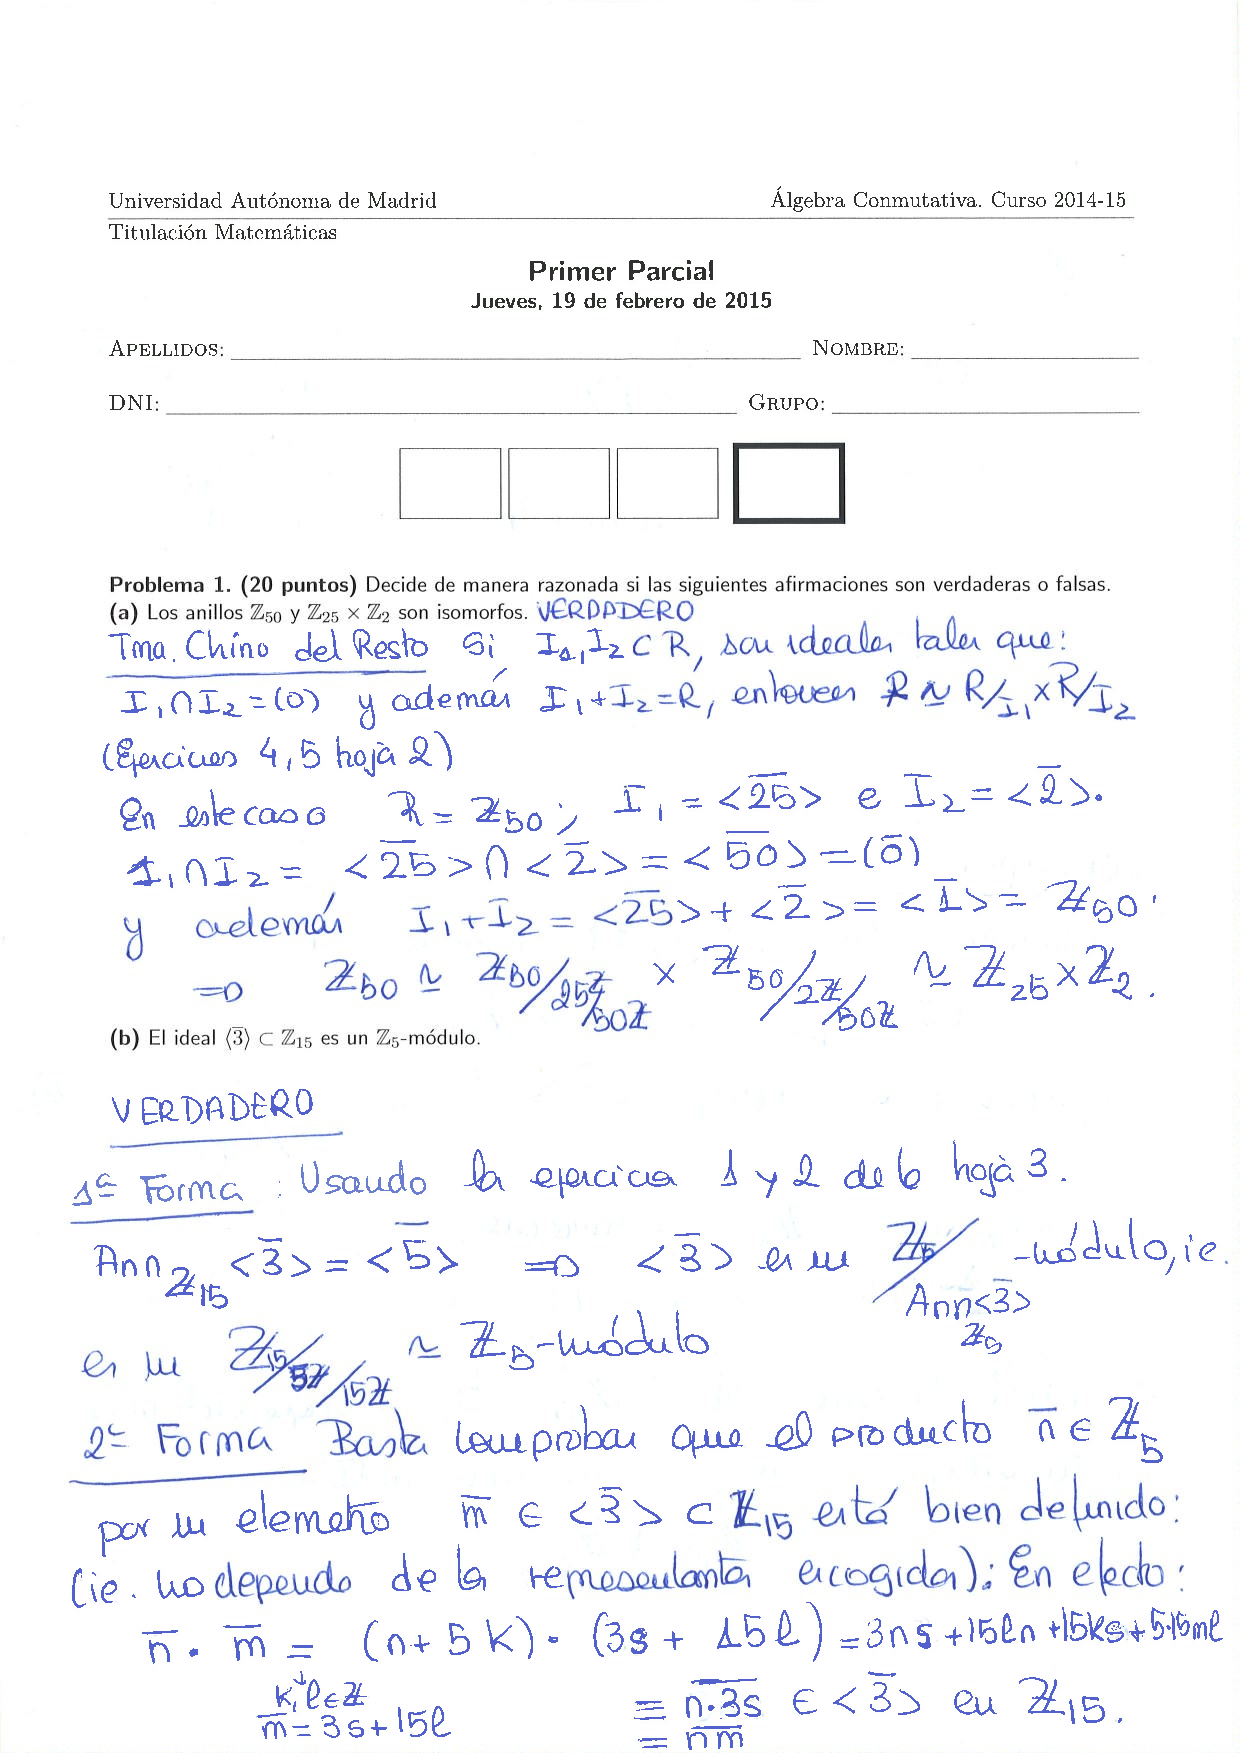
\includepdf[pages={1-4},scale=1]{pdf/_solucionesp1.pdf}

% Bibliografia
\nocite{reidAG,reidCA}
\bibliography{AlgebraConmutativa}{}

\printindex
\end{document}
